\documentclass[a4paper, 12pt]{article}
\def\MakeUppercaseUnsupportedInPdfStrings{\scshape}

%%% Работа с русским языком
\usepackage{cmap}					% поиск в PDF
\usepackage{mathtext} 				% русские буквы в формулах
\usepackage[T2A]{fontenc}			% кодировка
\usepackage[utf8]{inputenc}			% кодировка исходного текста
\usepackage[russian]{babel}	% локализация и переносы

%%% Дополнительная работа с математикой
\usepackage{amsmath,amsfonts,amssymb,amsthm,mathtools, amscd} % AMS
\usepackage{icomma} % "Умная" запятая: $0,2$ --- число, $0, 2$ --- перечисление

%% Номера формул
%\mathtoolsset{showonlyrefs=true} % Показывать номера только у тех формул, на которые есть \eqref{} в тексте.

%% Шрифты
\usepackage{euscript}	 % Шрифт Евклид
\usepackage{mathrsfs} % Красивый матшрифт

%% Поля
\usepackage[left=2cm,right=2cm,top=2cm,bottom=2cm,bindingoffset=0cm]{geometry}

%% Русские списки
\usepackage{enumitem}
\makeatletter
\AddEnumerateCounter{\asbuk}{\russian@alph}{щ}
\makeatother

%%% Работа с картинками
\usepackage{graphicx}  % Для вставки рисунков
\graphicspath{{images/}{images2/}}  % папки с картинками
\setlength\fboxsep{3pt} % Отступ рамки \fbox{} от рисунка
\setlength\fboxrule{1pt} % Толщина линий рамки \fbox{}
\usepackage{wrapfig} % Обтекание рисунков и таблиц текстом

%%% Работа с таблицами
\usepackage{array,tabularx,tabulary,booktabs} % Дополнительная работа с таблицами
\usepackage{longtable}  % Длинные таблицы
\usepackage{multirow} % Слияние строк в таблице
\usepackage[table,xcdraw]{xcolor} % Цветные таблицы

%% Красная строка
\setlength{\parindent}{2em}

%% Интервалы
\linespread{1}
\usepackage{multirow}

%% TikZ
\usepackage{tikz}
\usetikzlibrary{graphs,graphs.standard}

%% Верхний колонтитул
\usepackage{fancyhdr}
\pagestyle{fancy}

%% Перенос знаков в формулах (по Львовскому)
\newcommand*{\hm}[1]{#1\nobreak\discretionary{}
	{\hbox{$\mathsurround=0pt #1$}}{}}

%% Мои дополнения
\usepackage{booktabs} %Добавляет красивые таблицы по стандартам журналов
\usepackage{float} %Добавляет возможность работы с командой [H] которая улучшает расположение на странице
\usepackage{gensymb} %Красивые градусы
\usepackage{graphicx}               % Импорт изображений
\usepackage{caption} % Пакет для подписей к рисункам, в частности, для работы caption*
\usepackage{dsfont}
\usepackage{upgreek}    
\usepackage{wasysym}  
\usepackage{ifthen}
\usepackage[stable]{footmisc}
\usepackage{diagbox}
\usepackage{ tipa }
\usepackage{citeref}

\usepackage{hyperref}
\hypersetup{
	colorlinks,
	citecolor=black,
	filecolor=black,
	linkcolor=black,
	urlcolor=black
}

%%% Теоремы
\theoremstyle{plain}                    % Это стиль по умолчанию, его можно не переопределять.
\renewcommand\qedsymbol{$\blacksquare$} % переопределение символа завершения доказательства

\newtheorem{theorem}{Теорема}[section] % Теорема (счетчик по секиям)
\newtheorem{proposition}{Утверждение}[section] % Утверждение (счетчик по секиям)
\newtheorem{definition}{Определение}[section] % Определение (счетчик по секиям)
\newtheorem{corollary}{Следствие}[theorem] % Следстиве (счетчик по теоремам)
\newtheorem{problem}{Задача}[section] % Задача (счетчик по секиям)
\newtheorem*{remark}{Замечание} % Замечание
\newtheorem{lemma}{Лемма}[section] % Лемма (счетчик по секиям)

\newtheorem{example}{Пример}[section] % Пример
\newtheorem{counterexample}{Контрпример}[section] % Контрпример

\newtheorem{theorem_sub}{Теорема}[subsection]

\newcommand{\eqdef}{\stackrel{\mathrm{def}}{=}}
\newcommand{\ryad}{\sum\limits^{\infty}_{k = 0}}

%\newcommand*{\contfrac}[2]{%
	%{
	%	\rlap{$\dfrac{1}{\phantom{#1}}$}%
	%	\genfrac{}{}{0pt}{0}{}{#1+#2}%
	%}

\newcommand{\R}{\mathbb{R}}
\newcommand{\N}{\mathbb{N}}
\newcommand{\series}{\sum\limits_{k=1}^{\infty}}
\newcommand{\useries}{\sum\limits_{k=1}^{\infty} u_k}
\newcommand{\useriesl}{\sum\limits_{k=1}^{\infty} u_k < \infty}
\newcommand{\useriese}{\sum\limits_{k=1}^{\infty} u_k = \infty}
\newcommand{\auseries}{\sum\limits_{k=1}^{\infty} |u_k|}
\newcommand{\auseriesl}{\sum\limits_{k=1}^{\infty} |u_k| < \infty}
\newcommand{\auseriese}{\sum\limits_{k=1}^{\infty} |u_k| = \infty}
\newcommand{\sn}{\sum\limits_{k=1}^{n} u_k}
\DeclareMathOperator{\sgn}{\mathop{sgn}}

\newcommand{\te}{\ensuremath{\; \Rightarrow \;}}
\newcommand{\x}{\cdot}
\newcommand
{\un}[1]
{\ensuremath{\text{#1}}}
\newcommand{\eds}{\ensuremath{ \mathscr{E}}}
\newcommand{\ga}{\ensuremath{\gamma}}

\renewcommand {\ge}{\geqslant}
\renewcommand {\le}{\leqslant}
\renewcommand {\geq}{\geqslant}
\renewcommand {\leq}{\leqslant}
\renewcommand {\epsilon}{\varepsilon}
\newcommand{\RomanNumeralCaps}[1]
{\MakeUppercase{\romannumeral #1}}


\DeclareMathOperator{\cov}{cov}

\newenvironment{Definition}[2][]
{
	\vspace{1.2\baselineskip}
	\noindent\textbf{Определение}
	\ifthenelse{\equal{#1}{}}
	{}
	{	
		\textbf{(#1)}	
	}
	{\footnotesize [источник: #2]}
	
	\vspace{1.6mm} \small
	
}{\vspace{1.2\baselineskip}}


\newenvironment{Theorem}[2][]
{
	\vspace{1.2\baselineskip}
	\noindent\textbf{Теорема}
	\ifthenelse{\equal{#1}{}}
	{}
	{	
		\textbf{(#1)}	
	}
	{\footnotesize [источник: #2]}
	
	\vspace{1.6mm} \small
	
}{\vspace{1.2\baselineskip}}


\newenvironment{Proof}
{
	\noindent\textbf{\textit{Доказательство:}} \\
}{$\qed$\vspace{1.2\baselineskip}}


\newenvironment{Remark}[1]
{
	\vspace{1.2\baselineskip}
	\noindent\textbf{Замечание}
	{\footnotesize [источник: #1]}
	
	\vspace{1.6mm} \small
}{\vspace{1.2\baselineskip}}


\newenvironment{Proposal}[1]
{
	\vspace{1.2\baselineskip}
	\noindent\textbf{Предложение}
	{\footnotesize [источник: #1]}
	
	\vspace{1.6mm} \small
}{\vspace{1.2\baselineskip}}


\begin{document}

\newcommand{\HRule}{\rule{\linewidth}{0.7mm}} % Defines a new command for the horizontal lines, change thickness here
	
	\begin{center}
		\large\textbf{Московский Физико-Технический Институт}\\
		\large\textbf{(государственный университет)}
	
		\vfill
		
		\Large Дискретные случайные процессы\\[0.5cm] % Minor heading such as course title
		
		%----------------------------------------------------------------------------------------
		%	TITLE SECTION
		%----------------------------------------------------------------------------------------
		
		\HRule
		\\[0.4cm]
		{ \huge \bfseries Избранные темы}
		\\[0.4cm] % Title of your document
		\HRule
		\\[0.5cm]
		
		\ \\

		\vfill
		\hspace*{-0.8 cm}
\includegraphics[width=100 pt]{frkt_logo}\\
		\large Долгопрудный, 2023
	\end{center}

\newpage
\setcounter{page}{2}
\fancyfoot[c]{\thepage}
\fancyhead[L] {ДСП. Избранные темы}
%\fancyhead[R]{\rightmark}{0.5pt}
\fancyhead[R]{}

\tableofcontents{} %содержание

\newpage
% n-мерная функция распределения

\section{$n$-мерная функция распределения}

\textbf{Автор:} Артамонов Кирилл Сергеевич, Б-01-007

\subsection{Способы задания вероятностных мер на измеримых пространствах}
\label{par_3}

1. Измеримое пространство $(R, {B}(R))$. Пусть ${P}={P}(A)-$ вероятностная мера, определенная на борелевских множествах $A$ числовой прямой. Возьмем $A=(-\infty, x]$ и положим

$$
F(x)={P}(-\infty, x], \quad x \in R .
$$

Так определенная функция обладает следующими свойствами:

1) $F(x)$ - неубывающая функция;

2) $F(-\infty)=0, F(+\infty)=1$, где

$$
F(-\infty)=\lim _{x \downarrow-\infty} F(x), \quad F(+\infty)=\lim _{x \uparrow \infty} F(x)
$$

3) $F(x)$ непрерывна справа и имеет пределы слева в каждой точке $x \in R$.

Первое свойство очевидно, последние два вытекают из свойства непрерывности вероятностной меры.

\begin{definition}\label{def_1_par_3}
Всякая функция $F=F(x)$, удовлетворяющая перечисленным условиям 1)-3), называется функцией распределения (на числовой прямой $R$ ).
\end{definition}

Итак, каждой вероятностной мере ${P}$ на $(R, {B}(R))$ соответствует (в силу (1)) некоторая функция распределения. Оказывается, что имеет место и обратное утверждение. 

\begin{theorem}\label{theo_1_par_3}
Пусть $F=F(x)$ - некоторая функция распределения на числовой прямой $R$. Тогда на $(R, {B}(R))$ существует и притом единственная вероятностная мера ${P}$ такая, что для любых $-\infty \leqslant a<b<\infty$

$$
{P}(a, b]=F(b)-F(a)
$$
\end{theorem}

\subsubsection{Измеримое пространство $\left(R^{n}, {B}\left(R^{n}\right)\right)$.}

Как и в случае действительной прямой, предположим, что ${P}$ - некоторая вероятностная мера на $\left(R^{n}, {B}\left(R^{n}\right)\right)$.

Обозначим

$$
F_{n}\left(x_{1}, \ldots, x_{n}\right)={P}\left(\left(-\infty, x_{1}\right] \times \ldots \times\left(-\infty, x_{n}\right]\right),
$$

или, в более компактной форме,

$$
F_{n}(x)={P}(-\infty, x]
$$

где $x=\left(x_{1}, \ldots, x_{n}\right),(-\infty, x]=\left(-\infty, x_{1}\right] \times \ldots \times\left(-\infty, x_{n}\right]$.

Введем разностный оператор $\Delta_{a_{i} b_{i}}: R^{n} \rightarrow R$, действующий по формуле $\left(a_{i} \leqslant b_{i}\right)$

$$
\begin{aligned}
& \Delta_{a_{i} b_{i}} F_{n}\left(x_{1}, \ldots, x_{n}\right)=F_{n}\left(x_{1}, \ldots, x_{i-1}, b_{i}, x_{i+1}, \ldots, x_{n}\right)- \\
& -F_{n}\left(x_{1}, \ldots, x_{i-1}, a_{i}, x_{i+1}, \ldots, x_{n}\right) \text {. }
\end{aligned}
$$

Простой подсчет показывает, что

$$
\Delta_{a_{1} b_{1}} \ldots \Delta_{\alpha_{n} b_{n}} F_{n}\left(x_{1}, \ldots, x_{n}\right)={P}(a, b]
$$

где $(a, b]=\left(a_{1}, b_{1}\right] \times \ldots \times\left(a_{n}, b_{n}\right]$. Отсюда, в частности, видно, что, в отличие от одномерного случая, вероятность ${P}(a, b]$, вообще говоря, не равна разности $F_{n}(b)-F_{n}(a)$. Поскольку ${P}(a, b] \geqslant 0$, то из (7) следует, что для любых $a=\left(a_{1}, \ldots, a_{n}\right)$, $b=\left(b_{1}, \ldots, b_{n}\right)$

$$
\Delta_{a_{1} b_{1}} \ldots \Delta_{a_{n} b_{n}} F_{n}\left(x_{1}, \ldots, x_{n}\right) \geqslant 0
$$

Из непрерывности вероятности ${P}$ вытекает также, что $F_{n}\left(x_{1}, \ldots, x_{n}\right)$ непрерывна справа по совокупности переменных, т. е. если $x^{(k)} \downarrow x, x^{(k)}$ $=\left(x_{1}^{(k)}, \ldots, x_{n}^{(k)}\right)$, то

$$
F_{n}\left(x^{(k)}\right) \downarrow F_{n}(x), \quad k \rightarrow \infty
$$

Ясно также, что

$$
F_{n}(+\infty, \ldots,+\infty)=1 \quad \quad \text{и} \quad \quad \lim _{x \downarrow y} F_{n}\left(x_{1}, \ldots, x_{n}\right)=0
$$

если по крайней мере одна из координат у $y$ принимает значение $-\infty$.


\begin{definition}\label{def_2_par_3} Всякую функцию $F=F_{n}\left(x_{1}, \ldots, x_{n}\right)$, удовлетворяющую условиям (8)-(11), будем называть n-мерной функцией распределения (в пространстве $R^{n}$ ).
\end{definition}

Используя те же самые рассуждения, что и в теореме 1 , можно доказать справедливость следующего результата.


\begin{theorem}\label{theor_2_par_3}
Пусть $F=F\left(x_{1}, \ldots, x_{n}\right)$ - некоторая функция распределения в $R^{n}$. Тогда на $\left(R^{n}, {B}\left(R^{n}\right)\right)$ существует и притом единственная вероятностная мера ${P}$ такая, что

$$
{P}(a, b]=\Delta_{a_{1} b_{1}} \ldots \Delta_{a_{n} b_{n}} F_{n}\left(x_{1}, \ldots, x_{n}\right)
$$

Приведем некоторые примеры $n$-мерных функций распределения. Пусть $F^{1}, \ldots, F^{n}$ - одномерные функции распределения (на $R$ ) и

$$
F_{n}\left(x_{1}, \ldots, x_{n}\right)=F^{1}\left(x_{1}\right) \ldots F^{n}\left(x_{n}\right) .
$$

Ясно, что эта функция непрерывна справа и удовлетворяет условиям на функцию распределения. Нетрудно проверить также, что

$$
\Delta_{a_{1} b_{1}} \ldots \Delta_{a_{n} b_{n}} F_{n}\left(x_{1}, \ldots, x_{n}\right)=\prod\left[F^{k}\left(b_{k}\right)-F^{k}\left(a_{k}\right)\right] \geqslant 0 .
$$

Следовательно, $F_{n}\left(x_{1}, \ldots, x_{n}\right)$ - некоторая функция распределения.

Особо важен случай, когда

$$
F^{k}\left(x_{k}\right)= \begin{cases}0, & x_{k}<0 \\ x_{k}, & 0 \leqslant x_{k} \leqslant 1, \\ 1, & x_{k}>1 .\end{cases}
$$

В этом случае для всех $0 \leqslant x_{k} \leqslant 1, k=1, \ldots, n$,

$$
F_{n}\left(x_{1}, \ldots, x_{n}\right)=x_{1} \ldots x_{n} .
$$

Соответствующую этой $n$-мерной функции распределения вероятностную меру называют $n$-мерной мерой Лебега на $[0,1]^{n}$.
\end{theorem}


\subsubsection{Измеримое пространство $\left(R^{\infty}, {B}\left(R^{\infty}\right)\right)$.}
\begin{theorem}[Колмогорова о продолжении мер в $\left(R^{\infty}, {B}\left(R^{\infty}\right)\right)$]\label{theor_3_par_3} . Пyсть $P_{1}, P_{2}, \ldots$ - nocлeдовательность вероятностных мер на $(R, {B}(R)), \quad\left(R^{2}, {B}\left(R^{2}\right)\right)$, ..., обладающих свойством согласованности (16). Тогда существует и притом единственная вероятностная мера ${P}$ на $\left(R^{\infty}, {B}\left(R^{\infty}\right)\right)$ такая, что для каждого $n=1,2, \ldots$

$$
{P}\left({I}_{n}(B)\right)=P_{n}(B), \quad B \in {B}\left(R^{n}\right)
$$
\end{theorem}

\begin{proof} Пусть $B^{n} \in {B}\left(R^{n}\right)$ и ${I}_{n}\left(B^{n}\right)-$ цилиндр с «основанием» $B^{n}$. Припишем этому цилиндру меру ${P}\left({I}_{n}\left(B^{n}\right)\right)$, полагая ее равной $P_{n}\left(B^{n}\right)$

Покажем, что в силу условия согласованности такое определение является корректным, т. е. значение ${P}\left({F}_{n}\left(B^{n}\right)\right)$ не зависит от способа представления цилиндрического множества ${F}_{n}\left(B^{n}\right)$. В самом деле, пусть один и тот же цилиндр представлен двумя способами:

$$
{I}_{n}\left(B^{n}\right)={I}_{n+k}\left(B^{n+k}\right)
$$

Отсюда следует, что если $\left(x_{1}, \ldots, x_{n+k}\right) \in R^{n+k}$, то

$$
\left(x_{1}, \ldots, x_{n}\right) \in B \Leftrightarrow\left(x_{1}, \ldots, x_{n+k}\right) \in B^{n+k}
$$

\centering{и, значит}

$$
\begin{aligned}
& P_{n}\left(B^{n}\right)=P_{n+1}\left(\left(x_{1}, \ldots, x_{n+1}\right):\left(x_{1}, \ldots, x_{n}\right) \in B^{n}\right)=\ldots \\
& \ldots=P_{n+k}\left(\left(x_{1}, \ldots, x_{n+k}\right):\left(x_{1}, \ldots, x_{n}\right) \in B\right)=P_{n+k}\left(B^{n+k}\right) .
\end{aligned}
$$
\end{proof}

Обозначим ${A}\left(R^{\infty}\right)$ совокупность всех цилиндрических множеств $\widehat{B}^{n}=$ $={F}_{n}\left(B^{n}\right), B^{n} \in {B}\left(R^{n}\right), n=1,2 \ldots$ Нетрудно видеть, что ${A}\left(R^{\infty}\right)-$ алгебра. Пусть теперь $\widehat{B}^{1}, \ldots, \widehat{B}^{k}-$ непересекающиеся множества из ${A}\left(R^{\infty}\right)$. Без ограничения общности можно считать, что все они таковы, что для некоторого $n \widehat{B}_{i}={I}_{n}\left(B_{i}^{n}\right), i=1, \ldots, k$, где $B_{1}^{n}, \ldots, B_{k}^{n}$ - непересекающиеся множества из ${B}\left(R^{n}\right)$. Тогда

$$
{P}\left(\sum_{i=1}^{k} \widehat{B}_{i}\right)={P}\left(\sum_{i=1}^{k} {I}_{n}\left(B_{i}^{n}\right)\right)=P_{n}\left(\sum_{i=1}^{k} B_{i}^{n}\right)=\sum_{i=1}^{k} P_{n}\left(B_{i}^{n}\right)=\sum_{i=1}^{n} {P}\left(\widehat{B}_{i}\right),
$$

т. е. функция множеств ${P}-$ конечно-аддитивна на алгебре ${A}\left(R^{\infty}\right)$.

Покажем, что ${P}$ непрерывна в «нуле» (а, значит, и $\sigma$-аддитивна на ${A}\left(R^{\infty}\right)$;, т. е. если последовательность множеств $\widehat{B}_{n} \downarrow \varnothing$, $n \rightarrow \infty$, то ${P}\left(\widehat{B}_{n}\right) \rightarrow 0, n \rightarrow \infty$

Предположим противное, т. е. пусть $\lim _{n} {P}\left(\widehat{B}_{n}\right)=\delta>0$. Без ограничения общности можно считать, что последовательность $\left\{\widehat{B}_{n}\right\}$ такова, что

$$
\widehat{B}_{n}=\left\{x:\left(x_{1}, \ldots, x_{n}\right) \in B_{n}\right\}, \quad B_{n} \in {B}\left(R^{n}\right) .
$$

Воспользуемся следующим свойством вероятностных мер $P_{n}$ на $\left(R^{n}, {B}\left(R^{n}\right)\right)$ : если $B_{n} \in {B}\left(R^{n}\right)$, то для заданного $\delta>0$ можно найти такой компакт $A_{n} \in {B}\left(R^{n}\right)$, что $A_{n} \subseteq B_{n}$ и $P_{n}\left(B_{n} \backslash A_{n}\right) \leqslant \delta / 2^{n+1}$. Поэтому, если $\widehat{A}_{n}=\left\{x:\left(x_{1}, \ldots, x_{n}\right) \in A_{n}\right\}$, то

$$
{P}\left(\widehat{B}_{n} \backslash \widehat{A}_{n}\right)=P_{n}\left(B_{n} \backslash A_{n}\right) \leqslant \delta / 2^{n+1} .
$$

Образуем множество $\widehat{C}_{n}=\bigcap_{k=1}^{n} \widehat{A}_{k}$, и пусть $C_{n}$ таковы, что

$$
\widehat{C}_{n}=\left\{x:\left(x_{1}, \ldots, x_{n}\right) \in C_{n}\right\}
$$

Тогда, учитывая, что множества $\widehat{B}_{n}$ убывают, находим

$$
{P}\left(\widehat{B}_{n} \backslash \widehat{C}_{n}\right) \leqslant \sum_{k=1}^{n} {P}\left(\widehat{B}_{n} \backslash \widehat{A}_{k}\right) \leqslant \sum_{k=1}^{n} {P}\left(\widehat{B}_{k} \backslash \widehat{A}_{k}\right) \leqslant \delta / 2 .
$$

Но по предположению $\lim _{n} {P}\left(\widehat{B}_{n}\right)=\delta>0$, и, значит, $\lim _{n} {P}\left(\widehat{C}_{n}\right) \geqslant \delta / 2>0$. Покажем, что это противоречит тому, что $\widehat{C}_{n} \downarrow \varnothing$.

Действительно, выберем в множествах $\widehat{C}_{n}$ по точке $\hat{x}^{(n)}=\left(x_{1}^{(n)}, x_{2}^{(n)}, \ldots\right)$. Тогда для каждого $n \geqslant 1\left(x_{1}^{(n)}, \ldots, x_{n}^{(n)}\right) \in C_{n}$.

Пусть $\left(n_{1}\right)$ - некоторая подпоследовательность последовательности $(n)$ такая, что $x_{1}^{\left(n_{1}\right)} \rightarrow x_{1}^{0}$, где $x_{1}^{0}-$ некоторая точка в $C_{1}$. (Такая подпоследовательность существует, поскольку все $x_{1}^{\left(n_{1}\right)} \in C_{1}$, а $C_{1}-$ компакт.) Из последовательности $\left(n_{1}\right)$ выберем подпоследовательность $\left(n_{2}\right)$ такую, что $\left(x_{1}^{\left(n_{2}\right)}, x_{2}^{\left(n_{2}\right)}\right) \rightarrow\left(x_{1}^{0}, x_{2}^{0}\right) \in C_{2}$. Аналогичным образом пусть $\left(x_{1}^{\left(n_{k}\right)}, \ldots, x_{k}^{\left(n_{k}\right)}\right) \rightarrow$ $\rightarrow\left(x_{1}^{0}, \ldots, x_{k}^{0}\right) \in C_{k}$. Образуем, наконец, диагональную последовательность $\left(m_{k}\right)$, где $m_{k}$ есть $k$-й член в последовательности $\left(n_{k}\right)$. Тогда для любого $i=1,2, \ldots x_{i}^{\left(m_{k}\right)} \rightarrow x_{i}^{0}$ при $m_{k} \rightarrow \infty$, причем точка $\left(x_{1}^{0}, x_{2}^{0}, \ldots\right) \in \widehat{C}_{n}$ для любого $n=1,2, \ldots$, что, очевидно, противоречит предположению о том, что $\widehat{C}_{n} \downarrow \varnothing, n \rightarrow \infty$.

Итак, функция множеств ${P}$ на алгебре ${A}\left(R^{\infty}\right)$ является $\sigma$-аддитивной и, значит, по теореме Каратеодори может быть продолжена до (вероятностной) меры на $\left(R^{\infty}, {B}\left(R^{\infty}\right)\right)$.

\subsubsection{Измеримые пространства $\left(R^{T}, {B}\left(R^{T}\right)\right)$.}
 Пусть $T-$ произвольное множество индексов $t \in T$ и $R_{t}$ - числовая прямая, соответствующая индексу t. Рассмотрим произвольный конечный неупорядоченный набор $\tau=\left[t_{1}, \ldots, t_{n}\right]$ различных индексов $t_{i}, t_{i} \in T, n \geqslant 1$, и пусть $P_{\tau}$ - вероятностная мера на $\left(R^{\tau}, {B}\left(R^{\tau}\right)\right)$ с $R^{\tau}=R_{t_{1}} \times \ldots \times R_{t_{n}}$.

Будем говорить, что семейство вероятностных мер $\left\{P_{\tau}\right\}$, где $\tau$ пробегает множество всех конечных неупорядоченных наборов, является согласованныц, если для любых наборов $\tau=\left[t_{1}, \ldots, t_{n}\right]$ и $\sigma=\left[s_{1}, \ldots, s_{k}\right]$ таких, что $\sigma \subseteq \tau$

$$
\begin{aligned}
& P_{\sigma}\left\{\left(x_{s_{1}}, \ldots, x_{s_{k}}\right):\left(x_{s_{1}}, \ldots, x_{s_{k}}\right) \in B\right\}= \\
& =P_{\tau}\left\{\left(x_{t_{1}}, \ldots, x_{t_{n}}\right):\left(x_{s_{1}}, \ldots, x_{s_{k}}\right) \in B\right\}
\end{aligned}
$$

для любого $B \in {B}\left(R^{\sigma}\right)$.

\begin{theorem}[Колмогорова о продолжении мер в $\left(R^{T}, {B}\left(R^{T}\right)\right)$] Пусть $\left\{P_{\tau}\right\}$ - семейство согласованных вероятностных мер на $\left(R^{\tau}, {B}\left(R^{\tau}\right)\right)$. Тогда существует и притом единственная вероятностная мера ${P}$ на $\left(R^{T}, {B}\left(R^{T}\right)\right)$ такая, что 

$$
{P}\left({I}_{\tau}(B)\right)=P_{\tau}(B)
$$

для всех неупорядоченных наборов $\tau=\left[t_{1}, \ldots, t_{n}\right]$ различных индексов
$$
t_i \in T, B \in {B}\left(R^{T}\right) \quad \quad \text{и} \quad \quad {I}_{\tau}(B) = {x \in R^T : (\left(x_{t_{1}}, x_{t_{2}}, \ldots\right) \in B)} $$
\end{theorem}

\begin{proof} Пусть множество $\widehat{B} \in {B}\left(R^{T}\right)$. Согласно теореме~\ref{theor_2_par_3}, найдется не более чем счетное множество $S=\left\{s_{1}, s_{2}, \ldots\right\} \subseteq T$ такое, что $\widehat{B}=\left\{x:\left(x_{S_{1}}, x_{S_{2}}, \ldots\right) \in B\right\}$, где $B \in {B}\left(R^{S}\right), R^{S}=R_{S_{1}} \times R_{S_{2}} \times \ldots$ Иначе говоря, $\widehat{B}={I}_{S}(B)$ - цилиндрическое множество с «основанием» $B \in {B}\left(R^{S}\right)$.

На таких цилиндрических множествах $\widehat{B}={I}_{S}(B)$ определим функцию множеств ${P}$, полагая

$$
{P}\left({I}_{S}(B)\right)=P_{S}(B)
$$

где $P_{S}-$ та вероятностная мера, существование которой гарантируется теоремой~\ref{theor_3_par_3}.

Мы утверждаем, что $P$ - именно та мера, о существовании которой говорится в теореме. Чтобы установить это, надо, во-первых, проверить, что определение корректно, т. е. приводит к одному и тому же значению ${P}(\widehat{B})$ при разных способах представления $\widehat{B}$, и, во-вторых, что эта функция множеств счетно-аддитивна.

Итак, пусть $\widehat{B}={I}_{S_{1}}\left(B_{1}\right)$ и $\widehat{B}={I}_{S_{2}}\left(B_{2}\right)$. Ясно, что тогда $\widehat{B}={I}_{S_{1} \cup S_{2}}\left(B_{3}\right)$ с некоторым $B_{3} \in {B}\left(R^{S_{1} \cup S_{2}}\right)$, и поэтому достаточно лишь убедиться в том, что если $S \subseteq S^{\prime}$ и $B \in {B}\left(R^{S}\right)$, то $P_{S^{\prime}}\left(B^{\prime}\right)=P_{S}(B)$, где

$$
B^{\prime}=\left\{\left(x_{s_{1}^{\prime}}, x_{s_{2}^{\prime}}, \ldots\right):\left(x_{S_{1}}, x_{S_{2}}, \ldots\right) \in B\right\}
$$

c $S^{\prime}=\left\{s_{1}^{\prime}, s_{2}^{\prime}, \ldots\right\}, S=\left\{s_{1}, s_{2}, \ldots\right\}$.

Но в силу условия согласованности это равенство непосредственно вытекает из теоремы 3 , что и доказывает независимость значений ${P}(\widehat{B})$ от способа представления множества $\widehat{B}$.

Далее, для проверки свойства счетной аддитивности функции множеств ${P}$ предположим, что $\left\{\widehat{B}_{n}\right\}$ - некоторая последовательность попарно непересекающихся множеств из ${B}\left(R^{T}\right)$. Тогда найдется такое не более чем счетное множество $S \subseteq T$, что для любого $n \geqslant 1 \widehat{B}_{n}={I}_{S}\left(B_{n}\right)$, где $B_{n} \in {B}\left(R^{S}\right)$. Поскольку $P_{S}-$ вероятностная мера, то

$$
\begin{aligned}
& {P}\left(\sum \widehat{B}_{n}\right)={P}\left(\sum {I}_{S}\left(B_{n}\right)\right)=P_{S}\left(\sum B_{n}\right)=\sum P_{S}(B_n) = \sum{P}\left( {I}_{S}\left(B_{n}\right)\right) = \sum{P}\left(\widehat{B}_{n}\right)
\end{aligned}
$$


Наконец, требуемое свойство непосредственно следует из самой конструкции меры ${P}$.
\end{proof}


\subsection{Случайные элементы}
\label{par_5}

1. Наряду со случайными величинами в теории вероятностей и ее приложениях рассматривают случайные объекты более общей природы, например, случайные точки, векторы, функции, процессы, поля, множества, меры и т. д. В связи с этим желательно иметь понятие случайного объекта произвольной природы.


\begin{definition}
Пусть $(\Omega, {F})$ и $(E, {E})$ - два измеримых пространства. Будем говорить, что функция $X=X(\omega)$, определенная на $\Omega$ и принимающая значения в $E$, есть ${F} / {E}-$измеримая функция, или случайный элемент (со значениями в $E$ ), если для любого $B \in {E}$

$$
\{\omega: X(\omega) \in B\} \in {F} .
$$
\end{definition}

Иногда случайные элементы (со значениями в $E$ ) называют также E-значньми случайными величинами.

Рассмотрим частные случаи этого определения.

% Если $(E, {G})=(R, {B}(R))$, то определение случайного элемента совпадает с определением случайной величины (\S 4).

Пусть $(E, {E})=\left(R^{n}, {B}\left(R^{n}\right)\right)$. Тогда случайный Элемент $X(\omega)$ есть «случайная точка»в $R^{n}$. Если $\pi_{k}$ - проекция $R^{n}$ на $k$-ю координатную ось, то $X(\omega)$ можно представить в виде

$$
X(\omega)=\left(\xi_{1}(\omega), \ldots, \xi_{n}(\omega)\right)
$$

где $\xi_{k}=\pi_{k} \circ X$

Из условия вытекает, что $\xi_{k}$ - обычные случайные величины. Действительно, для любого $B \in {B}(R)$

$$
\begin{aligned}
& \left\{\omega: \xi_{k}(\omega) \in B\right\}= \\
& \begin{array}{l}
=\left\{\omega: \xi_{1}(\omega) \in R, \ldots, \xi_{k-1}(\omega) \in R, \xi_{k}(\omega) \in B, \xi_{k+1}(\omega) \in R, \ldots, \xi_{n}(\omega) \in R\right\}= \\
\quad=\{\omega: X(\omega) \in(R \times \ldots \times R \times B \times R \times \ldots \times R)\} \in {F},
\end{array}
\end{aligned}
$$

Поскольку множество $R \times \ldots \times R \times B \times R \times \ldots \times R \in {B}\left(R^{n}\right)$.

\begin{definition}
Всякий упорядоченный набор случайных величин $\left(\eta_{1}(\omega), \ldots, \eta_{n}(\omega)\right)$ будем называть $n$-мерным случайным вектором.
\end{definition}

В соответствии с этим определением всякий случайный элемент $X(\omega)$ со значениями в $R^{n}$ является $n$-мерным случайным вектором. Справедливо и обратное: всякий случайный вектор $X(\omega)=\left(\xi_{1}(\omega), \ldots, \xi_{n}(\omega)\right)$ есть случайный элемент в $R^{n}$. Действительно, если $B_{k} \in {B}(R), k=1, \ldots, n$, то

$$
\left\{\omega: X(\omega) \in\left(B_{1} \times \ldots \times B_{n}\right)\right\}=\prod_{k=1}^{n}\left\{\omega: \xi_{k}(\omega) \in R_{k}\right\} \in {F} .
$$

Но наименьшая $\sigma$-алгебра, содержащая множества $B_{1} \times \ldots \times B_{n}$, совпадает c ${B}\left(R^{n}\right)$. Тогда из очевидного обобщения леммы 1 из $\$ 4$ сразу получаем, что для любого $B \in {B}\left(R^{n}\right)$ множество $\{\omega: X(\omega) \in B\}$ принадлежит ${F}$.

Пусть $(E, {E})=({Z}, {B}({Z}))$, где ${Z}-$ множество комплексных чисел $z=x+i y, x, y \in R$, а ${B}({Z})$ - наименьшая $\sigma$-алгебра, содержащая множества вида
\newline
$\left\{z: z=x+i y, a_{1}<x \leqslant b_{1}, a_{2}<y \leqslant b_{2}\right\}$. 
\newline
Из предыдущего рассмотрения следует, что комплекснозначная случайная величина $Z(\omega)$ представляется в виде $Z(\omega)=X(\omega)+i Y(\omega)$, где $X(\omega)$ и $Y(\omega)-$ случайные величины. Поэтому $Z(\omega)$ называют также комплексными случайными величинами.

Пусть $(E, {E})=\left(R^{T}, {B}\left(R^{T}\right)\right)$, где $T$ - некоторое подмножество числовой прямой. В этом случае всякий случайный Элемент $X=X(\omega)$, представимый, очевидно, в виде $X=\left(\xi_{t}\right)_{t \in T}$ с $\xi_{t}=\pi_{t} \circ X$, называют случайной функцией с временным интервалом $T$.

Так же, как и для случайных векторов, устанавливается, что всякая случайная функция является в то же самое время случайным процессом в смысле следующего определения.

\begin{definition}\label{def_3_par_5}
 Пусть $T$ - некоторое подмножество числовой прямой. Совокупность случайных величин $X=\left(\xi_{t}\right)_{t \in T}$ называется случайным (стохастическим) процессом с временным интервалом $T$.

Если $T=\{1,2, \ldots\}$, то $X=\left(\xi_{1}, \xi_{2}, \ldots\right)$ называют случайным процессом с дискретным временем или случайной последовательностью.

Если $T=[0,1],(-\infty, \infty),[0, \infty), \ldots$, то $X=\left(\xi_{t}\right)_{t \in T}$ называют случайным процессом с непрерывным временем.
\end{definition}

\begin{definition} Пусть $X=\left(\xi_{t}\right)_{t \in T}-$ случайный процесс. Для каждого фиксированного $\omega \in \Omega$ функция $\left(\xi_{t}(\omega)\right)_{t \in T}$ называется реализацией или траекторией процесса, соответствующей исходу $\omega$.
\end{definition}

\begin{definition} Пусть $X=\left(\xi_{t}\right)_{t \in T}-$ случайный процесс. Вероятностная мера $P_{X}$ на $\left(R^{T}, {B}\left(R^{T}\right)\right)$ с

$$
P_{X}(B)={P}\{\omega: X(\omega) \in B\}, \quad B \in {B}\left(R^{T}\right)
$$

называется распределением вероятностей процесса $X$. Вероятности

$$
P_{t_{1}, \ldots, t_{n}}(B) \equiv {P}\left\{\omega:\left(\xi_{t_{1}}, \ldots, \xi_{t_{n}}\right) \in B\right\}
$$

c $t_{1}<t_{2}<\ldots<t_{n}, t_{i} \in T$, называются конечномерными вероятностями (или распределениями вероятностей). Функции

$$
F_{t_{1}, \ldots, t_{n}}\left(x_{1}, \ldots, x_{n}\right) \equiv {P}\left\{\omega: \xi_{t_{1}} \leqslant x_{1}, \ldots, \xi_{t_{n}} \leqslant x_{n}\right\}
$$

с $t_{1}<t_{2}<\ldots<t_{n}, t_{i} \in T$, называются конечномерными функциями распределения процесса $X=\left(\xi_{t}\right)_{t \in T}$.
\end{definition}

\subsection{Построение процесса с заданными конечномерными распределениями}
\label{par_9}

1. Пусть $\xi=\xi(\omega)$ - случайная величина, заданная на вероятностном пространстве $(\Omega, {F}, P)$ и

$$
F_{\xi}(x)={P}\{\omega: \xi(\omega) \leqslant x\}
$$

- ее функция распределения. Понятно, что $F_{\xi}(x)$ является функцией распределения на числовой прямой в смысле определения \ref{def_1_par_3}.

Поставим сейчас следующий вопрос. Пусть $F=F(x)-$ некоторая функция распределения на $R$. Спрашивается, существует ли случайная величина, имеющая функцию $F(x)$ своей функцией распределения?

Одна из причин, оправдывающих эту постановку вопроса, состоит в следующем. Многие утверждения теории вероятностей начинаются словами: «Пусть $\xi$ - случайная величина с функцией распределения $F(x)$, тогда...». Поэтому, чтобы утверждения подобного типа были содержательными, надо иметь уверенность, что рассматриваемый объект действительно существует. Поскольку для задания случайной величины нужно прежде всего задать область ее определения $(\Omega, {F})$, а для того, чтобы говорить о ее распределении, надо иметь вероятностную меру ${P}$ на $(\Omega, {F})$, то правильная постановка вопроса о существовании случайной величины с заданной функцией распределения $F(x)$ такова:

Существуют ли вероятностное пространство  $(\Omega, {F}, {P})$и случайная величина $\xi=\xi(\omega)$ на нем такие, что

$$
{P}\{\omega: \xi(\omega) \leqslant x\}=F(x) \text { ? }
$$

Покажем, что ответ на этот вопрос положительный и, в сущности, он содержится в теореме~\ref{theo_1_par_3}.

Действительно, положим

$$
\Omega=R, {F}={B}(R) .
$$

Тогда из теоремы \ref{theo_1_par_3} следует, что на $(R, {B}(R))$ существует (и притом единственная) вероятностная мера ${P}$, для которой ${P}(a, b]=F(b)-F(a)$, $a<b$.

Положим $\xi(\omega) \equiv \omega$. Тогда

$$
{P}\{\omega: \xi(\omega) \leqslant x\}={P}\{\omega: \omega \leqslant x\}={P}(-\infty, x]=F(x) .
$$

Таким образом, требуемое вероятностное пространство и искомая случайная величина построены.

2. Поставим теперь аналогичный вопрос для случайных процессов.

Пусть $X=\left(\xi_{t}\right)_{t \in T}-$ случайный процесс (в смысле определения \ref{def_3_par_5}), заданный на вероятностном пространстве $(\Omega, {F}, {P})$ для $t \in T \subseteq R$.

C физической точки зрения наиболее важной вероятностной характеристикой случайного процесса является набор $\left\{F_{t_{1}, \ldots, t_{n}}\left(x_{1}, \ldots, x_{n}\right)\right\}$ его конечномерных функций распределения

$$
F_{t_{1}, \ldots, t_{n}}\left(x_{1}, \ldots, x_{n}\right)={P}\left\{\omega: \xi_{t_{1}} \leqslant x_{1}, \ldots, \xi_{t_{n}} \leqslant x_{n}\right\}
$$

заданных для всех наборов $t_{1}, \ldots, t_{n}$ с $t_{1}<t_{2}<\ldots<t_{n}$.

Видно, что для каждого набора $t_{1}, \ldots, t_{n}$ с $t_{1}<t_{2}<\ldots<t_{n}$ функции $F_{t_{1}, \ldots, t_{n}}\left(x_{1}, \ldots, x_{n}\right)$ являются $n$-мерными функциями распределения (в смысле определения~\ref{def_2_par_3}) и что набор $\left\{F_{t_{1}, \ldots, t_{n}}\left(x_{1}, \ldots, x_{n}\right)\right\}$ удовлетворяет следующим условиям согласованности (\ref{par_3}):

$$
\begin{aligned}
F_{t_{1}, \ldots, t_{k}, \ldots, t_{n}}\left(x_{1}, \ldots, \infty, \ldots,\right. & \left.x_{n}\right)= \\
& =F_{t_{1}, \ldots, t_{k-1}, t_{k+1}, \ldots, t_{n}}\left(x_{1}, \ldots, x_{k-1}, x_{k+1}, \ldots, x_{n}\right) .
\end{aligned}
$$


\begin{theorem}[Колмогорова о существовании процесса]. Пусть $\left\{F_{t_{1}, \ldots, t_{n}}\left(x_{1}, \ldots, x_{n}\right)\right\}$, где $t_{i} \in T \subseteq R, t_{1}<t_{2}<\ldots<t_{n}, n \geqslant 1$, - заданное семейство конечномерных функций распределения, удовлетворяющих условиям согласованности (2). Тогда существуют вероятностное пространство $\left(\Omega, {F}\right.$, P) и случайный процесс $X=\left(\xi_{t}\right)_{t \in T}$ такие, что

$$
{P}\left\{\omega: \xi_{t_{1}} \leqslant x_{1}, \ldots, \xi_{t_{n}} \leqslant x_{n}\right\}=F_{t_{1}, \ldots, t_{n}}\left(x_{1}, \ldots, x_{n}\right) .
$$
\end{theorem}

\begin{proof} Положим

$$
\Omega=R^{T}, \quad {F}={B}\left(R^{T}\right),
$$

т. е. возьмем в качестве пространства $\Omega$ пространство действительных функций $\omega=\left(\omega_{t}\right)_{t \in T}$ с $\sigma$-алгеброй, порожденной цилиндрическими множествами.

Пусть $\tau=\left[t_{1}, \ldots, t_{n}\right], t_{1}<t_{2}<\ldots<t_{n}$. Тогда, согласно теореме~\ref{theor_2_par_3}, в пространстве $\left(R^{n}, {B}\left(R^{n}\right)\right)$ можно построить (и притом единственную) вероятностную меру $P_{\tau}$ такую, что

$$
P_{\tau}\left\{\left(\omega_{t_{1}}, \ldots, \omega_{t_{n}}\right): \omega_{t_{1}} \leqslant x_{1}, \ldots, \omega_{t_{n}} \leqslant x_{n}\right\}=F_{t_{1}, \ldots, t_{n}}\left(x_{1}, \ldots, x_{n}\right) .
$$

Из условий согласованности вытекает, что семейство $\left\{P_{\tau}\right\}$ также является согласованным. Согласно \ref{par_3}, на пространстве $\left(R^{T}, {B}\left(R^{T}\right)\right)$ существует вероятностная мера ${P}$ такая, что

$$
{P}\left\{\omega:\left(\omega_{t_{1}}, \ldots, \omega_{t_{n}}\right) \in B\right\}=P_{\tau}(B)
$$

для всякого набора $\tau=\left[t_{1}, \ldots, t_{n}\right], t_{1}<\ldots<t_{n}$.

Отсюда следует также, что выполнено условие требуемое условие. Таким образом, в качестве искомого случайного процесса $X=\left(\xi_{t}(\omega)\right)_{t \in T}$ можно взять процесс, определенный следующим образом:

$$
\xi_{t}(\omega)=\omega_{t}, \quad t \in T
$$
\end{proof}

\begin{remark}
Построенное вероятностное пространство $\left(R^{T}, {B}\left(R^{T}\right), {P}\right)$ часто называют каноническим, а такое задание случайного процесса - координатным способом построения процесса.
\end{remark}

\begin{corollary} Пусть $F_{1}(x), F_{2}(x), \ldots$ - последовательность одномерных функций распределения. Тогда существуют вероятностное пространство $(\Omega, {F}$, P) и последовательность независимых случайных величин $\xi_{1}, \xi_{2}, \ldots$ такие, что

$$
{P}\left\{\omega: \xi_{i}(\omega) \leqslant x\right\}=F_{i}(x)
$$
\end{corollary}

B частности, существует вероятностное пространство $(\Omega, {F}, {P})$, на котором определена бесконечная последовательность бернуллевских случайных величин. В качестве $\Omega$ можно здесь взять пространство

$$
\Omega=\left\{\omega: \omega=\left(a_{1}, a_{2}, \ldots\right), a_{i}=0 u \Omega u 1\right\}
$$

(ср. также с теоремой \ref{theor_2_par_3}).

Для доказательства следствия достаточно положить 
\newline
$F_{1, \ldots, n}\left(x_{1}, \ldots, x_{n}\right)$ $=F_{1}\left(x_{1}\right) \ldots F_{n}\left(x_{n}\right)$
\newline
и применить теорему \ref{theo_1_par_3} .



\begin{corollary} Пусть $T=\{0,1,2, \ldots\} \quad u\left\{P_{k}(x ; B)\right\}$ - семейство неотрицательных функций, определенных для $k \geqslant 1, x \in R, B \in {B}(R)$ и таких, ито функция $P_{k}(x ; B)$ есть вероятностная мера по $B$ (при фиксированных $k$ u ) и измерима по х (при фиксированных $k$ и $B$ ). Пусть, кроме того, $\pi=\pi(\cdot)$ - вероятностная мера на $(R, {B}(R))$.

Тогда можно построить вероятностное пространство $(\Omega, {F}, {P})$ с семейством случайных величин $X=\left\{\xi_{0}, \xi_{1}, \ldots\right\}$ на нем таких, что

$$
\begin{aligned}
{P}\left\{\xi_{0} \leqslant x_{0}, \xi_{1} \leqslant x_{1}, \ldots, \xi_{n}\right. & \left.\leqslant x_{n}\right\}= \\
& =\int_{-\infty}^{x_{0}} \pi\left(d y_{0}\right) \int_{-\infty}^{x_{1}} P_{1}\left(y_{0} ; d y_{1}\right) \ldots \int_{-\infty}^{x_{n}} P_{n}\left(y_{n-1} ; d y_{n}\right) .
\end{aligned}
$$
\end{corollary}




\newpage
% n-мерная плотность конечно мерного распределения случайного процесса

\section{n-мерная плотность конечно мерного распределения случайного процесса}

\textbf{Автор:} Паншин Артём Владимирович, Б-01-001

\subsection{n-мерная плотность распределения, определение и примеры [3]} % should be \cite{ShiryaevVeroyatnost1980}
Большой запас $n$-мерных функций распределения имеет вид
$$
F_n\left(x_1, \ldots, x_n\right)=\int_{-\infty}^{x_1} \ldots \int_{-\infty}^{x_n} f_n\left(t_1, \ldots, t_n\right) d t_1 \ldots d t_n,
$$
где $f_n\left(t_1, \ldots, t_n\right)$ - неотрицательные функции $\mathrm{c}$
$$
\int_{-\infty}^{\infty} \ldots \int_{-\infty}^{\infty} f_n\left(t_1, \ldots, t_n\right) d t_1 \ldots d t_n=1
$$
а интегралы понимаются в смысле Римана (и в более общем случае в смысле Лебега). Функции $f=f_n\left(t_1, \ldots, t_n\right)$ называют плотностями n-мерной функции распределения, п-мерной плотностью распределения вероятностей или просто п-мерными плотностями.
В случае $n=1$ функция
$$
f(x)=\frac{1}{\sqrt{2 \pi} \sigma} e^{-\frac{(x-m)^2}{2 \sigma^2}}, \quad x \in R
$$
c $\sigma>0$ есть плотность (невырожденного) гауссовского, или нормального, распределения. Существуют естественные аналоги этой плотности и в случае $n>1$.

Пусть $\mathbb{R}=\left| r_{i j}\right|$ - некоторая неотрицательно определенная симметрическая матрица порядка $n \times n$ :
$$
\begin{gathered}
\sum_{i, j=1}^n r_{i j} \lambda_i \lambda_j \geqslant 0, \quad \lambda_i \in R, \quad i=1, \ldots, n, \\
r_{i j}=r_{j i} .
\end{gathered}
$$
В том случае, когда $\mathbb{R}$ - положительно определенная матрица, ее детерминант $|\mathbb{R}| \equiv \operatorname{det} \mathbb{R}>0$, и, следовательно, определена обратная матрица $A=\left|a_{i j}\right|$. Тогда функция
$$
f_n\left(x_1, \ldots, x_n\right)=\frac{|A|^{1 / 2}}{(2 \pi)^{n / 2}} \exp \left\{-\frac{1}{2} \sum a_{i j}\left(x_i-m_i\right)\left(x_j-m_j\right)\right\},
$$
где $m_i \in R, i=1, \ldots, n$, обладает тем свойством, что интеграл (Римана) от нее по всему пространству равен 1, и, следовательно, в силу ее положительности она является плотностью.

Эта функция называется плотностью n-мерного (невырожденного) гауссовского, или нормального, распределения (с вектором средних значений $m=\left(m_1, \ldots, m_n\right)$ и матрицей ковариаций $\left.\mathbb{R}=A^{-1}\right)$.
В случае $n=2$ плотность $f_2\left(x_1, x_2\right)$ может быть приведена к виду
$$
 f\left(x_1, x_2\right)=\frac{1}{2 \pi \sigma_1 \sigma_2 \sqrt{1-\rho^2}} \exp \left\{-\frac{1}{2\left(1-\rho^2\right)} \times\right. \\
$$
$$
\left.\times\left[\frac{\left(x_1-m_1\right)^2}{\sigma_1^2}-2 \rho \frac{\left(x_1-m_1\right)\left(x_2-m_2\right)}{\sigma_1 \sigma_2}+\frac{\left(x_2-m_2\right)^2}{\sigma_2^2}\right]\right\} ,
$$
где $\sigma_i>0,|\rho|<1$.

\begin{remark} Как и в случае $n=1$, теорема 2 допускает обобщение на (аналогичным образом определяемые) меры Лебега-Стилтьеса в $\left(R^n, \mathscr{B}\left(R^n\right)\right)$ и обобщенные функции распределения в $R^n$. В том случае, когда обобщенная функция распределения $G_n\left(x_1, \ldots, x_n\right)$ равна $x_1 \ldots x_n$, соответствующая мера называется мерой Лебега на борелевских множествах пространства $R^n$. Ясно, что для нее
$$
\lambda(a, b]=\prod_{i=1}^n\left(b_i-a_i\right),
$$
т. е. мера Лебега «прямоугольника»
$$
(a, b]=\left(a_1, b_1\right] \times \ldots \times\left(a_n, b_n\right]
$$
\end{remark}

\subsection{Основные свойства $n$-мерных плотностей вероятности [8]} % should be  \cite{MaltsevBTRPR2014}
Плотности вероятности случайного процесса должны удовлетворять следующим условиям:

1. \textbf{Неотрицательность}: $f\left(x_1, t_1 ; x_2, t_2 ; \ldots ; x_n, t_n\right) \geq 0$;

2. \textbf{Нормировка}: $\int_{-\infty}^{\infty} \cdots \int_{-\infty}^{\infty} f\left(x_1, t_1 ; x_2, t_2 ; \ldots ; x_n, t_n\right) d x_1 d x_2 \ldots d x_n=1$;

3. \textbf{Симметрия}: $f\left(x_1, t_1 ; x_2, t_2 ; \ldots ; x_n, t_n\right)=f\left(x_2, t_2 ; x_1, t_1 ; \ldots ; x_n, t_n\right).$
Это свойство означает, что плотности вероятности симметричны относительно любых перестановок пар аргументов $\left(x_i, t_i\right), i=1,2, \ldots, n$. Например, для двумерной плотности вероятности $f\left(x_1, t_1 ; x_2, t_2\right) \equiv f\left(x_2, t_2 ; x_1, t_1\right)$. Это условие становится очевидным, если учесть, что содержание рассматриваемого события - совместное осуществление двух (или «n») неравенств $P\left\{\begin{array}{c}x_1 \leq x\left(t_1\right)<x_1+d x_1 \\ x_2 \leq x\left(t_2\right)<x_2+d x_2\end{array}\right\}$ не зависит от того, в каком порядке эти неравенства записываются:
$$
f\left(x_1, t_1 ; x_2, t_2\right) d x_1 d x_2 \equiv f\left(x_2, t_2 ; x_1, t_1\right) d x_1 d x_2 \equiv 
$$
$$ 
\equiv P\left\{X_i \leq X\left(t_i\right)<X_i+d X_i\right\}, \quad i=1,2
$$

4. \textbf{Согласованность.}
Данное свойство означает, что из плотности вероятности большей размерности всегда можно получить плотность вероятности меньшей размерности путем интегрирования по «лишним» аргументам. При любом $m<n$ имеем
$$f\left(x_1, t_1\right. ; \left.x_2, t_2 ; \ldots ; x_n, t_n\right)=\int_{-\infty}^{\infty} \cdots \int_{-\infty}^{\infty} f\left(x_1, t_1 ; x_2, t_2 ; \ldots ; x_n, t_n\right) d x_{m+1}$$$$ d x_{m+2} \ldots d x_n$$
Условие согласованности (как и предыдущие условия 1-3) в теории случайных процессов не является тривиальным повторением аналогичного соотношения для плотностей вероятности совокупности случайных величин. Оно ограничивает класс допустимых функций $f\left(x_1, t_1\right.$; $\left.x_2, t_2 ; \ldots ; x_n, t_n\right)$, поскольку интегрирование по $x_{m+1}, \ldots, x_n$ должно автоматически приводить к результату, не зависящему от параметров $t_{m+1}, t_{m+2}, \ldots, t_n$.

Перечисленные четыре свойства должны выполняться для плотности вероятности любого случайного процесса.


\newpage
% Гауссовские случайные процессы

\section{Гаусовские случайные процессы}

 \textbf{Автор:} Курицына Кристина Александровна, Б-01-009

\begin{definition} Случайный процесс $\{\xi(t), t \in T \}$
называется \textbf{гауссовским (нормальным)}, если все его конечномерные распределения являются нормальными, то есть для любых $k\geq 1$ и любых $t_1, \dots , t_k \in  T$ случайный вектор $(\xi(t_1 ), \dots , \xi(t_n))$ имеет нормальное распределение. \cite{NatanTeorVero2007}
\end{definition}

Напомним, что по определению вектор $\xi = (\xi_1, \dots , \xi_n)$ имеет нормальное распределение, если его характеристическая функция имеет вид:
\[\varphi_\xi (s) = exp(i\mu^T s - \frac{1}{2}s^T Rs)\]
для любого $ s \in \mathbb{R} ^{n} $. Здесь вектор $\mu = \mathbb{E} \xi \in \mathbb{R}^{n\times n}$ -  математическое ожидание вектора $ \xi$, а матрица
\[R = \mathbb{E} \xi \xi^T = \mathbb{E} (\xi - \mathbb{E} \xi)(\xi-\mathbb{E} \xi)^T \in \mathbb{R}^{n\times n}\]
- это корреляционная матрица вектора $\xi$. Если нормальный вектор имеет математическое ожидание $\mu$ и корреляционную матрицу $R$, то пишут, что $\xi \in N(\mu , R)$. \cite{NatanTeorVero2007}

То есть действительный случайный процесс $\xi (t)$, $t \in T$ называется гауссовским, если его характеристическая функция имеет следующий вид:
\[\Psi _\xi (z_1, \dots, z_k ; t_1, \dots, t_k ) = M\left\{exp\left(i\sum_{j = 1}^{k} z_j \xi(t_j) \right)\right\} = \]
\[= exp\left(i\sum_{j=1}^{k} z_j m_\xi (t_j) - \frac{1}{2} \sum_{l=1}^{k} \sum_{j=1}^{k} R_\xi (t_l , t_j )z_l z_j \right)\]
где $z_j$ - произвольные вещественные числа, а $t_j \in T$ и
\[m_\xi (t_j) = M\{\xi (t_j)\}, \qquad  R_\xi (t_l, t_j) = \textbf{cov} \{\xi(t_l), \xi(t_j)\}\]

Если обозначить через $(a, b) = \sum_{l=1}^{k} a_j b_j$ скалярное произведение векторов $a, b \in \mathbb{R}^{k}$, то характеристическую функцию можно представить в виде
\[\Psi_\xi (z; t_1, \dots, t_k) = exp\left( i(z, m_\xi) - \frac{1}{2} (R(_\xi z, z) \right),\]

где $z=\{z_1, \dots, z_k\}^{*} , m_\xi = \{ m_\xi (t_1), \dots, m_\xi(t_k)\}^{*}, R_\xi = \{R_\xi (t_i, t_j) \}_{i,j=1,\dots,k}$

$\newline$
То есть характеристичекая функция полностью определяет распределение совокупности случайных величин. \cite{ShiryaevVeroyatnost1}

\subsection*{Свойства гауссовских векторов}

 \begin{enumerate}
   \item Каждая компонента нормального вектора $\xi \in N(\mu, R)$ имеет нормальное распределение, причем $\xi_j \in N(\mu_j , R_{jj})$. Обратное неверно! То есть если у некоторого случайного вектора все компоненты по отдельности имеют нормальное распределение, то это значит, что вектор целиком имеет нормальное распределение. \cite{NugmanovBRP2014}
   $\newline$
   \textit{Дело в том, что совместное распределение компонент вектора в общем случае не определяется их частными распределениями. Однако если у слуайного вектора компоненты независимы в совокупности и имеют нормальное распределение, то тогда и вектор имеет нормальное распределение.}
   \item Гауссовский случайный вектор $\eta = \{\eta_1, \dots, \eta_k\}^{*}$ с математическим ожиданием $m_\eta$ и ковариационной матрицей $R_\eta$ имеет плотность распределения $p_\eta (x)$ тогда и только тогда, когда матрица $R_\eta$ - невырожденная, то есть $det[R_\eta] > 0$. В этом случае плотность распределения имеет следующий вид
    \[p_\eta (x) = (2\pi)^{-k/2} (det[R_\eta])^{-1/2} exp \left( - \frac{1}{2} (x - m_\eta)(R_\eta)^{-1} (x - m_\eta) \right) \]

    Таким образом если матрица $R_\xi = \{R_\xi (t_i, t_j )\}_{i,j=1,\dots,k}$ положительно определена, то совместное распределение сечений $\{ \xi(t_1), \dots, \xi(t_k)\}$ имеет плотность вероятности
    \[p_\xi (x; t_1, \dots, t_k) = (2\pi)^{-k/2} (det[R_\xi])^{-1/2} exp \left( - \frac{1}{2} (x - m_\xi)(R_\xi)^{-1} (x - m_\xi) \right) \]

    Если же матрица $R$ вырождена, то плотности распределения у вектора нет. В этом случае найдется вектор $c \ne 0$ такой, что $Rc = 0$б то есть $R$ имеет линейно зависимые столбцы и строки. Из этого следует, что компоненты вектора линейно связнаны, то есть вероятностная мера сконцентрирована на подпространстве меньшей размерности, а не на всем пространстве $\mathbb{R}^{n}$. \cite{ShiryaevVeroyatnost1}

    \item Пусть $\xi \in N(\mu, R), \xi \in \mathbb{R}^{n}$. Тогда для любой матрицы $A \in \mathbb{R}^{k\times n}$ (необязательно невырожденной и даже необязательно квадратной) вектор $A\xi$ тоже будет нормальным, причем  $A\xi \in N(A\mu, ARA^T)$. \cite{NugmanovBRP2014}

    \item Вектор $\xi$ является нормальным тогда и только тогда, когда любая линейная комбинация его компонент дает нормальную случайную величину или константу, и все его компоненты некоррелированы. \cite{ShiryaevVeroyatnost1}

    \item Компоненты нормального случайного вектора некоррелированы тогда и только тогда, когда независимы. \cite{NugmanovBRP2014}
    $\newline$
    \textit{Здесь нужно обратить внимание на то, что речь идет именно о компонентах нормального вектора, а не просто о нормальных случайных величинах. Просто нормальные случайные величины могут быть и некоррелированными, и зависимыми. Но если случайные величины не только нормальные, но и являются компонентами нормального вектора (более сильное свойство), то тогда из их некоррелированности следует их независимость.}

    \item Семейство конечномерных гауссовских распределений, соответствующее семейству характеристических функций $\Psi_\xi$, удовлетворяет условиям 1-6 теоремы Колмогорова.Таким образом, произвольный набор $\{\xi(t_1), \dots,\xi(t_k)\}$ сечений гауссовского случайного процесса является случайным вектором с гауссовским распределением. Также подчеркнем, что все эти распределения \textbf{согласованы} (см. лекцию о т. Колмогорова) \cite{ShiryaevVeroyatnost1}

    \item Из определения гауссовского процесса следует, что семейство его конечномерныз распределений полностью определяется двумя моментными характеристиками: математическим ожиданием и ковариационной функцией. \cite{ShiryaevVeroyatnost1}

 \end{enumerate}

\subsection*{Винеровский процесс}


\begin{definition} Гауссовский случайный процесс $\{\xi(t), t \geq 0 \}$ с непрерывным временем и моментными характеристиками 
\[M\{\xi(t)\} = 0 \quad \textbf{cov}\{\xi(t), \xi(s)\} = min(t, s) \quad t, s \geq 0\]
и выходящий из нуля, то есть $\xi(0) = 0$, называется \textbf{стандартным винеровским процессом} (или процессом броуновского движения). Это важнейший пример нормального случайного процесса. \cite{ShiryaevVeroyatnost1}
\end{definition}
$\newline$
$\newline$
Рассмотрим свойства винеровского процесса, которые можно вывести непосредственно из определения.
$\newline$
\begin{enumerate}
    \item Приращения процесса броуновского движения на непересекающихся промежутках времени независимы. \cite{ShiryaevVeroyatnost1}

    
    \textit{Покажем это и найдем распределение произвольного приращения.}
    $\newline$
    Прежде всего заметим, что совокупность приращений процесса броуновского движения $\xi(t_1) - \xi(t_0), \xi(t_2) - \xi(t_1), \dots, \xi(t_k) - \xi(t_{k-1})$, где $0 = t_0 < t_1 < \dots < t_k$ и $\xi(t_0) = 0$, имеет гауссовское распределение в силу гауссовости случайного вектора $\{\xi(t_1), \xi(t_2), \dots, \xi(t_k)\}^{*}$, поэтому для доказательства независимости приращений достаточно установить их некоррелированность. Итак, для мометнов времени $t_i < t_j$ верно
    \[\textbf{cov}\{\xi(t_i) - \xi(t_{i-1}), \xi(t_j) - \xi(t_{j-1})\} = \newline\]
    \[= min(t_i, t_j) - min(t_i, t_{j-1}) - min(t_{i-1}, t_j) + min (t_{i-1}, t_{j-1}) = 0\]

    что означает некоррельрованность приращений процесса $\xi(t)$ на промежутках $[t_{i-1}, t_i]$ и $[t_{j-1}, t_j]$.
    $\newline$
    Как уже отмечалось, приращение $\xi(t) - \xi(s)$ имеет гауссовское распределение, поэтому
    \[\xi(t) - \xi(s) \sim N(0; |t-s|)\]
    так как $M\{\xi(t) - \xi(s)\} = 0$ и $D\{\xi(t) - \xi(s) \} = t + s - 2min(t, s) = |t - s|$

    \item Найдем плотность конечномерного распределения процесса броуновского движения. \cite{ShiryaevVeroyatnost1}
    \[\eta_1 = \xi(t_1) - \xi(t_0), \eta_2 = \xi(t_2) - \xi(t_1), \dots, \eta_k = \xi(t_k) - \xi(t_{k-1})\]
    где $0 = t_0 < t_1 < \dots < t_k $
    $\newline$
    Поскольку $\xi(t_0) = 0$, то
    \[\xi(t_1) = \eta_1, \xi(t_2) = \eta_1 + \eta_2,  \dots, \xi(t_k) = \eta_1 + \dots + \eta_k\]

    Пусть $p_\eta$ - плотность распределения вектора $\eta = \{\eta_1, \dots, \eta_k\}^{*}$, а $p_{\eta_i}$ - плотность распределения приращения $\eta_i$. Тогда плотность распределения вектора $\xi = \{\xi(t_1), \dots, \xi(t_k)\}^{*}$ равна
    \[p_\xi (x_1, \dots, x_k; t_1, \dots, t_k) = p_\eta (x_1, x_2 - x_1, \dots, x_k - x_{k-1}) = \newline\]
    \[p_{\eta_1} (x_1) p_{\eta_2}(x_2 - x_1)\dots p_{\eta_k}(k_k - x_{k-1})\]

    где первое равенство следует из того, что якобиан преобразования $\eta \to \xi$ по модулю 1, а второе получено с учетом независимости случайных величин $\eta_i$. Тогда из свойств 1 следует
    \[p_\xi (x_1, \dots, x_k; t_1, \dots, t_k) = \prod_{i=1}^{k} \frac{1}{\sqrt{2\pi |t_i - t_{i-1}|}} exp \left\{ -\frac{(x_i - x_{i-1})^2}{2|t_i - t_{i-1}|} \right\}\]
    где $t_0 = 0, x_0 = 0$


    В приложениях весьма часто приходится иметь дело с \textbf{n-мерными гауссовскими процесами}, где $n>1$. По аналогии с введенным ранее определением гауссовского процесса мы можем назвать процесс  $\xi(t) \in \mathbb{R}^{n} , t \in T$ гауссовским, если при любых $t_1, \dots, t_k \in T, k \geq 1,  (n \times k)$ - мерный случайный вектор $\eta = \{ \xi^* (t_1), \dots, \xi^* (t_k)\}^{*}$ имеет гауссовское $(n \times k)$ - мерное распределение. Все свойства такого процесса полностью определяются n-мерной функцией математического ожидания $m_\xi (t)$ и $(n \times n)$ - мерной (то есь матричной) ковариационной функцией $R_\xi (t, s)$, которая вычисляется следующим образом \cite{ShiryaevVeroyatnost1}:
    \[R_\xi (t, s) = M\left\{ (\xi(t) - m_\xi(t))(\xi(s) - m_\xi(s))^* \right\} = M\left\{\xi(t)\xi^* (s)\right\} - m_\xi (t)m^* _\xi (s)\]

\end{enumerate}



\newpage
% Моментные характеристики второго порядка (математическое ожидание, дисперсия, ковариацион- ная функция, корреляционная функция).

\section{Моментные характеристики второго порядка для случайных процессов}

\textbf{Автор:} Гончаренко Валентина Павловна, Б-01-009

\subsection{Моменты}
\cite{ShamarovDRP11} $\alpha$-й \textbf{абсолютный момент распределения} ($\alpha \in \mathds{R}$) $\mu$ -- это выражение $\int\limits_{\mathds{R}}^{} |x|^\alpha \mu(dx)$. Если $\alpha$ - четное целое, то $\int\limits_{\mathds{R}}^{} x^\alpha \mu(dx)$ тоже называется $\alpha$-ым \textbf{моментом распределения}, но не абсолютным.

\begin{center}
\textbf{Неравество Коши-Буняковского}    
\end{center}

Пусть $\mu: \mathfrak{A} \rightarrow [0,N] (N < \infty); \mu$ -- $\sigma$-аддитивна на $\sigma$-алгебре $\mathfrak{A}$ с единицей $E = \bigcup \mathfrak{A} = \mathfrak{A}.$

\begin{proposition} если $f: E \rightarrow \mathds{R}$ (измерима), $\int\limits_{E}^{} f^2 \mu < \infty$, то $\int\limits_{E}^{} |f| \mu < \infty$.
\end{proposition}

\begin{proof} 
\ \\
\indent$\odot\quad|f| \leqslant max (1, f^2) \leqslant 1 + f^2$ 

$\odot\quad0 \leqslant f_{\pm} \leqslant |f|$

$\odot\quad \text{ч.т.д.}$
\end{proof}

\begin{proposition} если еще и $g: E \rightarrow \mathds{R}$ (измерима), $\int\limits_{E}^{} g^2 \mu < \infty$, то $ \exists \int\limits_{E}^{} fg \mu$ и $|\int\limits_{E}^{} fg \mu| \leqslant \sqrt{\int\limits_{E}^{} f^2 \mu} \sqrt{\int\limits_{E}^{} g^2 \mu}$ 
\end{proposition}

\begin{proof} 
\ \\
\indent$\odot\quad$ $0 \leqslant (f \pm \lambda g)^2 = f^2 \pm 2 \lambda fg + \lambda^2 g^2$, $\forall \lambda \in \mathds{R}$

$\odot\quad$ $|fg| = |f||g| = \sqrt{|f|^2 |g|^2} \leqslant \dfrac{1}{2} (f^2 + g^2)$

$\odot\quad$ $0 \leqslant \int\limits_{E}^{} (f \pm \lambda g)^2 \mu \equiv \lambda^2 \int\limits_{E}^{} g^2 \mu \pm 2\lambda \int\limits_{E}^{} fg \mu + \int\limits_{E}^{} f^2 \mu$ 

$\odot\quad$ $\dfrac{D}{4} \leqslant 0$: $(\int\limits_{E}^{} fg \mu)^2 - (\int\limits_{E}^{} g^2 \mu)(\int\limits_{E}^{} f^2 \mu) \leqslant 0$

$\odot\quad$ \text{Заменяем $f$ на $|f|$, $g$ на $|g|$:}\quad $|\int\limits_{E}^{} fg \mu| \leqslant \int\limits_{E}^{} |f||g| \mu \leqslant ||f||_{L_{2} (\mu)}||g||_{L_{2} (\mu)}$

$\odot\quad$ $||f||_{L_{\text{p}} (\mu)} = \sqrt[p]{\int\limits_{E}^{} |f|^p \mu}$

$\odot\quad$ \text{ч.т.д.} 
\end{proof}

\subsection{Математическое ожидание}

\cite{ShamarovDRP11} $\forall t \in T$ \textbf{математическое ожидание} вещественной случайной величины $\upxi_\text{t}$ с распределением $\mathds{P}_\text{t} \equiv \mathds{P}_\text{\{t\}}$ (будем рассматривать одномерное распределение для удобства выкладок) - это функция $\int\limits_{\mathds{R}}^{} x\mathds{P}_\text{t}(dx)$, если функция $f \equiv id\mathds{R}: \mathds{R} \ni x \rightarrow f(x) = x$ интегрируема в смысле Лебега по $\mathds{P}_\text{t}$.

\begin{example}$\rho_\text{\{t\}} (x) = \dfrac{1}{\pi (x^2 + 1)}$ -- величина с данной плотностью распределения не имеет математического ожидания (распределение Коши).
\end{example}


\begin{corollary}(из неравенства Коши-Буняковского:) $\int x^2 \mathds{P_\text{t}} (dx) < \infty \Longrightarrow \int |x| \mathds{P_\text{t}} (dx) \equiv |\int 1 \cdot |x| \cdot \mathds{P_\text{t}} (dx)| \leqslant \sqrt{\int 1^2 \mathds{P_\text{t}}} \sqrt{\int x^2 \mathds{P_\text{t}}} \Longrightarrow \exists \int x \mathds{P_\text{t}} (dx) = \mathds{E}\upxi_\text{t} \equiv \mathds{M}\upxi_\text{t}$ -- математическое ожидание случайной величины.
\end{corollary}

\subsection{Дисперсия}

\cite{ShamarovDRP11} Если 2-й момент существует для распределения $\mathds{P_\text{t}}$, то $\int (x - \mathds{E}\upxi_\text{t})^2 \mathds{P_\text{t}} = \mathds{D}\upxi_\text{t}$ -- \textbf{дисперсия} в момент времени $t$. 

$\mathds{D}\upxi_\text{t} = \int (x - \mathds{E}\upxi_\text{t})^2 \mathds{P_\text{t}} = \int x^2 \mathds{P_\text{t}} - (\mathds{E}\upxi_\text{t})^2 = \mathds{E}({\upxi_\text{t}})^2 - (\mathds{E}\upxi_\text{t})^2$, то есть для вычисления дисперсии случайной величины нужно из математического ожидания её квадрата вычесть квадрат её математического ожидания.

\begin{remark} в случае процесса среднее значение и дисперсия в любой момент времени (если они существуют) являются функциями $T \rightarrow \mathds{R}$. 
\end{remark}
 
\subsection{Ковариационная функция}

\cite{ShamarovDRP11} Пусть $t \in T \longmapsto \mathds{D}\upxi_\text{t} \in \mathds{R}$ -- конечная функция, тогда \textbf{ковариацией} процесса называется функция 
\begin{equation*}
    T^2 \equiv T \times T \ni (s,t) \longmapsto Cov(\upxi_\text{s}, \upxi_\text{t}) \equiv \left\{
    \begin{aligned}
        & \int\limits_{{\mathds{R}}^2}^{} (x - \mathds{E}\upxi_\text{s})(x - \mathds{E}\upxi_\text{t}) \mathds{P_\text{\{s,t\}}} (dx,dy) & \text{, если } t \neq s \\
        & \mathds{D}\upxi_\text{s} = \mathds{D}\upxi_\text{t} & \text{, если } t = s \\
    \end{aligned}
    \right.
\end{equation*}

Равносильное обозначение: $Cov(\upxi_\text{s}, \upxi_\text{t}) = \mathds{E}((\upxi_\text{s} - \mathds{E}\upxi_\text{s})(\upxi_\text{t} - \mathds{E}\upxi_\text{t}))$. 

\vspace{4pt}

 \begin{definition}~\cite{MillerRPET2001} Пусть $t_0 \in T$ -- фиксированный момент. Случайная величина $\upxi_{\text{t}_0}(w) = \upxi(t_0, w)$ называется \textbf{сечением} случайного процесса в точке $t_0 \in T$.
\end{definition}

 \begin{definition}~\cite{MillerRPET2001} Неслучайная функция $R_{\xi}(t, \tau), t, \tau \in T$, определяемая соотношением
$$
\begin{aligned}
& R_{\xi}(t, \tau)=\mathbf{c o v}\{\xi(t), \xi(\tau)\}=\mathbf{M}\left\{\left(\xi(t)-m_{\xi}(t)\right)\left(\xi(\tau)-m_{\xi}(\tau)\right)\right\}= \\
& =\mathbf{M}\{\xi(t) \xi(\tau)\}-m_{\xi}(t) m_{\xi}(\tau)=\int_{-\infty}^{\infty} \int_{-\infty}^{\infty} x_{1} x_{2} d F_{\xi}\left(x_{1}, x_{2} ; t, \tau\right)-m_{\xi}(t) m_{\xi}(\tau),
\end{aligned}
$$
называется \textbf{ковариационной} функцией случайного процесса $\xi(t)$.
\end{definition}

 \begin{remark}~\cite{MillerRPET2001} При любых $t, \tau \in T$ функция $R_{\xi}(t, \tau)$ численно равна ковариации сечений случайного процесса $\xi_{t}(\omega)$ и $\xi_{\tau}(\omega)$ в точках $t, \tau \in T$ и характеризует степень линейной зависимости между сечениями. Для вычисления $R_{\xi}(t, \tau)$ необходимо знать двумерное распределение $F_{\xi}\left(x_{1}, x_{2} ; t, \tau\right)$ процесса $\xi(t)$. Заметим также, что

$$
D_{\xi}(t)=R_{\xi}(t, t), \quad t \in T
$$

Из неравенства Коши-Буняковского следует, что для существования $m_{\xi}(t)$, $D_{\xi}(t)$ и $R_{\xi}(t, \tau)$ при всех $t, \tau \in T$ достаточно выполнения условия

$$
\mathbf{M}\left\{|\xi(t)|^{2}\right\}<\infty \quad \forall t \in T \quad \quad (*)
$$
\end{remark}

 \begin{remark}~\cite{MillerRPET2001} Если распределения $F_{\xi}(x ; t)$ и $F_{\xi}\left(x_{1}, x_{2} ; t, \tau\right)$ имеют плотности распре- деления $p_{\xi}(x ; t)$ и $p_{\xi}\left(x_{1}, x_{2} ; t, \tau\right)$, то

$$
\begin{gathered}
m_{\xi}(t)=\int_{-\infty}^{\infty} x p_{\xi}(x ; t) d x, \quad D_{\xi}(t)=\int_{-\infty}^{\infty} x^{2} p_{\xi}(x ; t) d x-m_{\xi}^{2}(t) \\
R_{\xi}(t, \tau)=\int_{-\infty}^{\infty} \int_{-\infty}^{\infty} x_{1} x_{2} p_{\xi}\left(x_{1}, x_{2} ; t, \tau\right) d x_{1} d x_{2}-m_{\xi}(t) m_{\xi}(\tau)
\end{gathered}
$$
\end{remark}

 \begin{definition}{\cite{MillerRPET2001}} Случайный процесс $\xi(t)$, $t \in T$, удовлетворяющий условию $(*)$, называется процессом с конечными моментами второго порядка или \textbf{гильбертовым} случайным процессом.
\end{definition}

 \begin{definition}~\cite{MillerRPET2001} Пусть $\xi(t)=X(t)+i Y(t)-$ комплексный процесс, где $X(t), Y(t), t \in T$ - некоторые действительные случайные процессы, а $i^{2}=-1$. Если 

$$
\mathbf{M}\left\{|\xi(t)|^{2}\right\}=\mathbf{M}\{\xi(t) \overline{\xi(t)}\}=\mathbf{M}\left\{X^{2}(t)+Y^{2}(t)\right\}<\infty \quad \forall t \in T,
$$
то процесс $\xi(t)$ называется \textbf{комплексным гильбертовым процессом}.

Функция

$$
R_{\xi}(t, \tau)=\mathbf{M}\left\{\left(\xi(t)-m_{\xi}(t)\right) \overline{\left(\xi(\tau)-m_{\xi}(\tau)\right)}\right\}, \quad t, \tau \in T,
$$
где $\overline{\{\cdot\}}$ означает комплексное сопряжение, называется \textbf{ковариационной функцией комплексного случайного процесса} $\xi(t)$.
\end{definition}

 \begin{definition}~\cite{MillerRPET2001} Пусть заданы два комплексных процесса $\xi(t)$, $\eta(t), t \in T$. Детерминированная функция

$$
R_{\xi \eta}(t, \tau)=\operatorname{\textbf{cov}}\{\xi(t), \eta(\tau)\}=\mathbf{M}\left\{\left(\xi(t)-m_{\xi}(t)\right) \overline{\left(\eta(\tau)-m_{\eta}(\tau)\right)}\right\}, \quad t, \tau \in T
$$
называется \textbf{взаимной ковариационной функцией процессов} $\xi$ и $\eta$.
\end{definition}

 \begin{remark}~\cite{MillerRPET2001} Функция $R_{\xi \eta}(t, \tau)$ существует, если $\xi(t)$ и $\eta(t)-$ гильбертовы процессы.
\end{remark}

\subsection{Корреляционная функция}

\cite{ShamarovDRP11} $\pluto\text{:} \quad T^2 = T \times T \ni (s,t) \longmapsto \dfrac{Cov(\upxi_\text{s}, \upxi_\text{t})}{\sqrt{\mathds{D}\upxi_\text{s}} \sqrt{\mathds{D}\upxi_\text{t}}}$





\newpage
% Белый шум с дискретным временем

\section{Белый шум с дискретным временем}	

\textbf{Автор:} Лабашкин Глеб Александрович, Б-01-007

\subsection*{1. Нормальный случайный вектор} 

\begin{definition} Невырожденным нормальным (гауссовским) случайным вектором  $\vec{\xi} = (\xi_1, \xi_2, \dots, \xi_n)^T$
называется случайный вектор, обладающий плотностью распределения вероятностей вида:
$$\rho_{\vec{\xi}}(x_1, x_2, \dots, x_n) = \rho_{\vec{\xi}}(\vec{x}) = 
k \exp(\displaystyle\frac{1}{2}(\vec{x} - \vec{b})^T A (\vec{x} - \vec{b})),$$
где $A$ -- симметричная положительно определённая матрица,
$k$ -- нормировочный коэффициент, $b$ -- неслучайный вектор. \cite{GasnikovLectionsRP} 
\end{definition}

Осуществим некоторые преобразования. Известно, что для каждой симметричной матрицы $A$
существует ортогональная матрица $C$, такая, что: $$ C^T A C = D = \mathrm{diag}(d_1, d_2, \dots, d_n) ,$$
где $d_i > 0 ,~ i = \overline{1, n}$ в силу положительной определённости матрицы $A$. 
Введём матрицу \break $B = C D^{-1/2}$ и вектор $\vec{z}$,
удовлетворяющий преобразованию: $$\vec{x} - \vec{b} = B \vec{z} ,$$
$$ D^{-1/2} = \mathrm{diag}(\frac{1}{\sqrt{d_1}}, \frac{1}{\sqrt{d_2}}, \dots, \frac{1}{\sqrt{d_n}}) .$$
C учётом данного преобразования:
$$ (\vec{x} - \vec{b})^T A (\vec{x} - \vec{b}) =  \vec{z}^T B^T A B \vec{z} = 
\vec{z}^T D^{-1/2} C^T A C D^{-1/2} \vec{z} = \vec{z}^T \vec{z}.$$
Якобиан преобразования:
$$J(\vec{x}, \vec{z}) = \left\lvert \frac{\partial{x_i}}{\partial{z_j}} \right\rvert = \det(B).$$
Запишем плотность распределения $f_{\vec{\xi}}$ случайного вектора $\vec{\xi}$ в переменных $\vec{z}$:
$$ f_{\vec{\xi}}(z_1, z_2, \dots, z_n) = f_{\vec{\xi}}(\vec{z}) =
k \det(B) \exp(-\frac{1}{2} \vec{z}^T \vec{z}) = k \det(B) \exp(-\frac{1}{2} \sum_{i = 1}^{n} z_i^2) .$$
Используя интеграл Пуассона $\displaystyle\int_{-\infty}^{+\infty} e^{-t^2} dt = \sqrt{\pi}$ и условие нормировки
$\displaystyle\int_{\mathbb{R}^n} f_{\vec{\xi}}(\vec{z}) d\vec{z} = 1$, выразим коэффициент $k$:
$$ \int_{\mathbb{R}^n} k \det(B) \exp(-\frac{1}{2} \vec{z}^T \vec{z}) d\vec{z} = 
(\sqrt{2\pi})^n k \det(B) = 1 ~ \Rightarrow ~ k = \frac{1}{(\sqrt{2\pi})^n \det(B)} .$$
Таким образом, плотность распределения принимает вид:
$$ f_{\vec{\xi}}(\vec{z}) = \frac{1}{(\sqrt{2\pi})^n} \exp(-\frac{1}{2} \sum_{i = 1}^{n} z_i^2) .$$
Из этой формулы мы можем видеть, что соответсвующий ранее данному определению нормальный случайный вектор
посредством линейной замены сводится к случайному вектору,
каждая из компонент которого имеет стандартное нормальное распределение: \\\\
$$\xi_i \in N(0, 1) ,~ f_{\xi_i}(z_i) = \frac{1}{\sqrt{2\pi}} \exp(-\frac{1}{2} z_i^2) ,~ i = \overline{1, n} ,$$
$$ f_{\vec{\xi}}(\vec{z}) = f_{\xi_1}(z_1) f_{\xi_2}(z_2) \dots f_{\xi_n}(z_n) .$$ 

\begin{remark} Обратное в общем случае неверно. \\
Если каждая из компонент случайного вектора имеет нормальное распределение, это ещё не означает,
что сам вектор будет гауссовским. Однако, это справедливо для случая,
когда компоненты вектора независимы в совокупности. \\\\
\end{remark}


\subsection*{2. Белый шум с дискретным временем}

\begin{definition} Нормальным (гауссовским) случайным процессом называется случайный процесс $\xi(t), t \in T$,
все конечномерные распределения которого нормальны. Это означает, что любой случайный вектор вида
$(\xi(t_1), \xi(t_2), \dots, \xi(t_n))^T ,~ n \in \mathbb{N} ,~ t_i \in T ,~ i = \overline{1, n}$
является нормальным (гауссовским) случайным вектором. \cite{NatanTeorVero2007} \\
\end{definition}

Рассматриваем множество $T \in \{ \mathbb{N}, \mathbb{N}_0 = \mathbb{N} \cup \{0\} \}$.
Пусть $\mathscr{P}_{fin}(T) =  \{ \mathfrak{t} \subset T \mid Card(\mathfrak{t}) \in \mathbb{N} \}$,
где $Card(\mathfrak{t})$ -- кардинальное число (или же мощность) множества $\mathfrak{t}$.
Это означает, что $\mathscr{P}_{fin}(T)$ является системой
всех конечных непустых поднможеств $\mathfrak{t}$ множества $T$.
Тогда элементы любого такого подмножества $\mathfrak{t} \in \mathscr{P}_{fin}(T)$ могут быть пронумерованы:
$\mathfrak{t} = \{ t_1 < t_2 < \dots < t_{Card(\mathfrak{t})} \}$.
$t_i \in \mathfrak{t}, i = \overline{1, Card(\mathfrak{t})}$ представляют собой моменты времени,
в которые осуществляется измерение некоторого физического процесса, создающего белый шум.
Для ясности изложения, можно говорить, что мы осуществляем запись шума водопада (который довольно близок к белому).
Измеряемой случайной величиной $\xi_i \equiv \xi_{t_i} \equiv \xi(t_i)$ в таком случае будет
отклонение мембраны микрофона записывающего устройства в момент времени $t_i$.
С целью получения нормального процесса, положим, что $\xi_i$ распределены по Гауссу
(хоть в контексте нашего примера это и нефизично) и независимы в совокупности:
$$ \rho_{\xi_i}(x) = \frac{1}{\sqrt{2\pi}} e^{-x^2/2} ,~ i = \overline{1, Card(\mathfrak{t})} .$$

\begin{definition} Случайный процесс $\xi(t), t \in T$,
удовлетворяющий сформулированным выше условиям, будем называть гауссовским белым шумом с дискретным временем. \cite{ShamarovDRP} \\
\end{definition}

\noindent Тогда не составляет труда выписать вероятностную меру для процесса:
$$\forall B \in \mathscr{B}(\mathbb{R}^{\mathfrak{t}}) ~ \mathbb{P}_{\xi}^{\mathfrak{t}}(B) \equiv 
\mathbb{P}_{\xi_1, \xi_2, \dots, \xi_{Card(\mathfrak{t})}}(B) = 
\int_{\vec{x} \in B} \frac {exp(-\Vert \vec{x} \Vert ^2 / 2)} {(\sqrt{2\pi}) ^ {Card(\mathfrak{t})}}
Leb_{\mathbb{R}^{\mathfrak{t}}}(d\vec{x}) ,$$ 
где $\mathscr{B}(\mathbb{R}^{\mathfrak{t}})$ -- борелевская сигма-алгебра на $\mathbb{R}^{\mathfrak{t}}$, 
$Leb_{\mathbb{R}^{\mathfrak{t}}}$ -- мера Лебега на $\mathbb{R}^{\mathfrak{t}}$,
$\Vert \vec{x} \Vert ^2 = \sum_{i = 1}^{Card(\mathfrak{t})} x_i^2$. \\

\begin{remark} Для построения случайного процесса белого шума в качестве маргинальных распределний
$\xi(t_i)$ вовсе не обязательно было полагать нормальное распеределние. Как известно из физики, белый шум характерен
равномерным распределением его спектральных составляющих. Это достигается не за счёт конкретного вида распределения
процесса $\xi$, а благодаря независимости (а если быть строгим, некоррелированности) значений,
измеряемых в разные моменты времени $t_i \neq t_j$, что будет продемонстрировано в следующем разделе. \\\\
\end{remark}


\subsection*{3. Белый шум в терминах стационарных последовательностей}

\begin{definition} Последовательность случайных величин $\xi \equiv \{ \xi_n \}_{n \in \mathbb{Z}}$
с $\mathbb{E}|\xi_n|^2 < \infty ,~ n \in \mathbb{Z}$ называется стационарной в широком смысле,
если для всех $n \in \mathbb{Z}$
$$ \mathbb{E}\xi_n = \mathbb{E}\xi_0 ,$$
$$ R(n) \equiv \mathrm{cov}(\xi_n, \xi_0) = \mathrm{cov}(\xi_{k+n}, \xi_k) ~ \forall k \in \mathbb{Z} .$$
$R(n)$ называется ковариационной функцией. \cite{ShiryaevVeroyatnost1980} \\
\end{definition}

Рассмотрим последовательность $\xi \equiv \{ \xi_n \}$ ортонормированных случайных величин $\xi_n$:
${\mathbb{E}\xi_n = 0}$, $\mathbb{E}\xi_i\xi_j = \delta_{ij}$, где $\delta_{ij}$ -- символ Кронекера.
Данная последовательность очевидно является стационарной и
$$ R(n) = \begin{cases} 1 ,~ n = 0 \\ 0 ,~ n \neq 0 \end{cases} .$$
Функция $R(n)$ может быть представлена в виде:
$$ R(n) = \int_{-\pi}^{\pi} e^{i \lambda n} dF(\lambda) ,$$
$$ F(\lambda) = \int_{-\pi}^{\lambda} f(\nu) d\nu ,~ f(\lambda) \equiv \frac{1}{2\pi} ,~ \lambda \in [ -\pi, \pi ) .$$
Здесь $F(\lambda)$ является функцией распределения,
а $f(\lambda) \equiv \displaystyle\frac{1}{2\pi}$ -- её спектральной плотностью,
которая постоянна на непрерывном промежутке $\lambda \in [ -\pi, \pi )$.
В этом смысле можно сказать, что последовательность $\xi \equiv \{ \xi_n \}$
"составлена из гармоник $\lambda$, интенсивность которых одинакова".
Именно это обстоятельство и послужило поводом называть данную последовательность белым шумом.



\newpage
% Модель авто регрессии - скользящего среднего 

\section{Модель авторегрессии скользящего среднего}

\textbf{Автор:}  Волков Вадим Леонидович, Б-01-007

\subsection{Белый шум}
Пусть $\varepsilon=\left(\varepsilon_{n}\right)$ - последовательность ортонормированных случайных величин, \\ $\mathbb{E} \varepsilon_{n}=0, ~ \mathbb{E} \varepsilon_{i} \varepsilon_{j}=\delta_{i j}$, где $\delta_{i j}-$ символ Кронекера. Понятно, что такая последовательность является стационарной и

$$
R(n)= \begin{cases}1, & n=0 \\ 0, & n \neq 0\end{cases}
$$

Отметим, что эта функция $R(n)$ может быть представлена в виде

$$
R(n)=\int_{-\pi}^{\pi} e^{i \lambda n} d F(\lambda)
\eqno(1)
$$

где

$$
F(\lambda)=\int_{-\pi}^{\lambda} f(\nu) d \nu, \quad f(\lambda)=\frac{1}{2 \pi}, \quad-\pi \leqslant \lambda<\pi .
\eqno(2)
$$


\subsection{Последовательности скользящего среднего} 
Отправляясь от белого шума $\varepsilon=\left(\varepsilon_{n}\right)$, образуем новую последовательность

$$
\xi_{n}=\sum_{k=-\infty}^{\infty} a_{k} \varepsilon_{n-k}
\eqno(3) 
$$

где $a_{k}$ - комплексные числа такие, что $\sum\limits_{k=-\infty}^{\infty} \left|a_{k}\right|^{2}<\infty$.

В том частном случае, когда все $a_{k}$ с отрицательными индексами равны нулю и, значит,

$$
\xi_{n}=\sum_{k=0}^{\infty} a_{k} \varepsilon_{n-k}
$$

Последовательность $\xi=\left(\xi_{n}\right)$ называют последовательностью одностороннего скользящего среднего. Если к тому же все $a_{k}=0$ при $k>p$, т. е. если

$$
\xi_{n}=a_{0} \varepsilon_{n}+a_{1} \varepsilon_{n-1}+\ldots+a_{p} \varepsilon_{n-p}
\eqno(4)
$$

то $\xi=\left(\xi_{n}\right)$ называется последовательностью скользящего среднего порядка $p$

Для последовательности (4) ковариационная функция $R(n)$ имеет вид $\\ R(n)=\int_{-\pi}^{\pi} e^{i \lambda n} f(\lambda) d \lambda$, где спектральная плотность равна

$$
f(\lambda)=\frac{1}{2 \pi}\left|P\left(e^{-i \lambda}\right)\right|^{2}
\eqno(5)
$$

с

$$
P(z)=a_{0}+a_{1} z+\ldots+a_{p} z^{p}
$$

Покажем, почему это так.  $F_{\varepsilon}(\lambda)-$ ассоциируется с белым шумом. 

$R(n)=\int_{-\pi}^{\pi} e^{i \lambda n} d F(\lambda) =
\sum\limits_{k=-\infty}^{\infty} a_{k} \int_{-\pi}^{\pi} e^{i \lambda (n-k)} d F_{\varepsilon}(\lambda)  = \lim\limits_{N\to\infty} \sum\limits_{k=-N}^{N} a_{k} \int_{-\pi}^{\pi} e^{i \lambda (n-k)} d F_{\varepsilon}(\lambda) = \lim\limits_{N\to\infty} \int_{-\pi}^{\pi} (\sum\limits_{k=-N}^{N} a_{k} e^{-ik\lambda}) e^{in\lambda} d F_{\varepsilon}(\lambda) = \int_{-\pi}^{\pi} (\sum\limits_{k=-\infty}^{\infty} a_{k} e^{-ik\lambda}) e^{in\lambda} d F_{\varepsilon}(\lambda) 
= \int_{-\pi}^{\pi} e^{in\lambda} P(e^{-i\lambda}) d F_{\varepsilon}(\lambda) $

\subsection{Авторегрессионная схема}
Пусть снова $\varepsilon=\left(\varepsilon_{n}\right)-$ белый шум. Будем говорить, что случайная последовательность $\xi=\left(\xi_{n}\right)$ подчиняется авторегрессионной схеме порядка $q$, если для $n \in \mathbf{Z}$

$$
\xi_{n}+b_{1} \xi_{n-1}+\ldots+b_{q} \xi_{n-q}=\varepsilon_{n}
\eqno(6)
$$

При каких условиях на коэффициенты $b_{1}, \ldots, b_{q}$ можно утверждать, что уравнение (6) имеет стационарное решение? Чтобы ответить на этот вопрос, рассмотрим сначала случай $q=1$ :

$$
\xi_{n}=\alpha \xi_{n-1}+\varepsilon_{n}
\eqno(7)
$$

где $\alpha=-b_{1}$. Если $|\alpha|<1$, то нетрудно проверить, что стационарная последовательность $\tilde{\xi}=\left(\tilde{\xi}_{n}\right)$ с

$$
\tilde{\xi}_{n}=\sum_{j=0}^{\infty} \alpha^{j} \varepsilon_{n-j}
\eqno(8)
$$

является решением уравнения (7). (Ряд в правой части (8) сходится в среднеквадратическом смысле.) Покажем теперь, что в классе стационарных последовательностей $\xi=\left(\xi_{n}\right)$ (с конечным вторым моментом) это решение является единственным. В самом деле, из (7) последовательными итерациями находим, что

$$
\xi_{n}=\alpha \xi_{n-1}+\varepsilon_{n}=\alpha\left[\alpha \xi_{n-2}+\varepsilon_{n-1}\right]+\varepsilon_{n}=\ldots=\alpha^{k} \xi_{n-k}+\sum_{j=0}^{k-1} \alpha^{j} \varepsilon_{n-j}
$$

Отсюда следует, что

$$
\mathbb{E}\left[\xi_{n}-\sum_{j=0}^{k-1} \alpha^{j} \varepsilon_{n-j}\right]^{2}=\mathbb{E}\left[\alpha^{k} \xi_{n-k}\right]^{2}=\alpha^{2 k} \mathbb{E} \xi_{n-k}^{2}=\alpha^{2 k} \mathbb{E} \xi_{0}^{2} \rightarrow 0, \quad k \rightarrow \infty .
$$

Таким образом, при $|\alpha|<1$ стационарное решение уравнения (7) существует и представляется в виде одностороннего скользящего среднего (8).

Аналогичный результат имеет место и в случае произвольного $q>1$ : если все нули полинома

$$
Q(z)=1+b_{1} z+\ldots+b_{q} z^{q}
\eqno(9)
$$

лежат вне единичного круга, то уравнение авторегрессии (6) имеет, и притом единственное, стационарное решение, представимое в виде одностороннего скользящего среднего. При этом ковариационная функция $R(n)$ представима в виде

$$
R(n)=\int_{-\pi}^{\pi} e^{i \lambda n} d F(\lambda), \quad F(\lambda)=\int_{-\pi}^{\lambda} f(\nu) d \nu
\eqno(10)
$$

где

$$
f(\lambda)=\frac{1}{2 \pi} \cdot \frac{1}{\left|Q\left(e^{-i \lambda}\right)\right|^{2}} .
\eqno(11)
$$

Покажем, почему это так. $F_{\varepsilon}(\lambda)-$ ассоциируется с белым шумом.    

$\sum\limits_{l=0}^{q} b_{l} \xi_{n-q} = \int_{-\pi}^{\pi} ( \sum\limits_{l=0}^{q} b_{l} e^{i \lambda (n-l)}) d F(\lambda) = \int_{-\pi}^{\pi} e^{in \lambda}\varphi(\lambda) d F(\lambda) = \int_{-\pi}^{\pi} e^{in \lambda} d F_{\varepsilon}(\lambda),  \newline \text{где } \varphi(\lambda) = \sum\limits_{l=0}^{q} b_{l} e^{-il\lambda}$

В частном случае $q=1$ из (7) легко находим, что $\mathrm{E} \xi_{0}=0$,

$$
\mathrm{E}\left|\xi_{0}\right|^{2}=\frac{1}{1-|\alpha|^{2}}, \quad R(n)=\frac{\alpha^{n}}{1-|\alpha|^{2}}, \quad n \geqslant 0
$$

$(R(n)=\overline{R(-n)}$ для $n<0)$. При этом

$$
f(\lambda)=\frac{1}{2 \pi} \cdot \frac{1}{\left|1-\alpha e^{-i \lambda}\right|^{2}} .
$$



\subsection{Смешанная модель авторегрессии и скользящего среднего}
Если предположить, что в правой части уравнения (6) вместо $\varepsilon_{n}$ стоит величина $a_{0} \varepsilon_{n}+a_{1} \varepsilon_{n-1}+\ldots+a_{p} \varepsilon_{n-p}$, то получим так называемую смешанную модель авторегрессии и скользящего среднего порядка $(p, q)$ :

$$
\xi_{n}+b_{1} \xi_{n-1}+\ldots+b_{q} \xi_{n-q}=a_{0} \varepsilon_{n}+a_{1} \varepsilon_{n-1}+\ldots+a_{p} \varepsilon_{n-p}
\eqno(12)
$$

При тех же предположениях относительно нулей полинома $Q(z)$, что и в примере авторегрессионной схемы, уравнение (12) имеет стационарное решение $\xi=\left(\xi_{n}\right)$, для которого ковариационная функция равна $R(n)=\int_{-\pi}^{\pi} e^{i \lambda n}  d F(\lambda)$ с $F(\lambda)=\int_{-\pi}^{\lambda} f(\nu) d \nu$, где

$$
f(\lambda)=\frac{1}{2 \pi}\left|\frac{P\left(e^{-i \lambda)}\right.}{Q\left(e^{-i \lambda}\right)}\right|^{2}
$$


\newpage
% Метод моментов для определения уравнений относительно математического ожидания и дисперсии (модель авторегрессии - скользящего среднего)


\section{Метод моментов для определения уравнений относительно математического ожидания и дисперсии (модель авторегрессии --- скользящего среднего)}

\textbf{Автор:} Отмахов Артем Денисович, Б-01-001

\subsection{Введение}
\begin{itemize}
    \item Все случайные величины (СВ) заданы на общем вероятностном пространстве $(\Omega, \mathscr{F}, \mathbb{P})$
    \item Для некоторой случайной последовательности (СП) $\{X_n\}$ вводим следующие обозначения:
    $$
        m_X(n) = \mathbb{M}(X_n)
    $$
    $$
        D_X(n) = \mathbb{D}(X_n) = \mathbf{cov}(X_n,~X_n) = \mathbb{M}((X_n - m_X(n))(X_n - m_X(n))^*)
    $$
    \item $\{\xi_n\}$ --- многомерная СП, т.е. $\xi_n \in \mathbb{R}^p$ при каждом $n \geq 0$
    \item Последовательность независимых СВ $\{\varepsilon_n\}$, $\varepsilon_n \in \mathbb{R}^q$ при $n \geq 1$: $\varepsilon_n$ --- стандартный $q$-мерный белый шум, т.е. $m_{\varepsilon}=0$, $D_{\varepsilon}=I$
    \item $\eta \in \mathbb{R}^p$ --- случайный вектор начальных условий
    \item $A_n \in \mathbb{R}^{p \times p}$, $B_n \in \mathbb{R}^{p \times q}$ --- известные неслучайные матрицы
    \item $\{\eta, \varepsilon_1, \dots, \}$ являются независимыми в совокупности
\end{itemize}


\subsection{Уравнение моментов для авторегрессии (АР) первого порядка}
\begin{definition} 
	СП $\{\xi_n,~n \geq 0\}$ удовлетворяет \textit{многомерному линейному разностному стохастическому уравнению с начальным условием} $\eta$, если
	\begin{equation}
	    \label{eq:recurrent}
	    \begin{cases}
	        \xi_n = A_n\xi_{n-1} + B_n\varepsilon_n, ~~ n \geq 1,\\
	        \xi_0 = \eta,
	    \end{cases}
	\end{equation}
\end{definition}
Рекуррентные соотношения \eqref{eq:recurrent} позволяют провести моделирование СП $\{\xi_n\}$, а также вычислить моментные характеристики первого и второго порядка $m_{\xi}(n)$ и $D_{\xi}(n)$ при заданных характеристиках $\{\varepsilon_n\}$ и начальном условии $\eta$.
\vspace{1mm}

\begin{theorem} 
	Если СП $\xi_n$  удовлетворяет системе \eqref{eq:recurrent}, то для $m_\xi(n)$ и $D_\xi(n)$ выполнено:
	\begin{equation}
	    \label{eq:method_of_moments}
	    \begin{cases}
	        m_\xi(n) = A_n m_\xi(n-1) + B_n m_\varepsilon(n), n \geq 1,\\
	        m_\xi(0) = m_\eta,\\
	        D_\xi(n) = A_n D_\xi(n-1) A_n^* + B_n D_\varepsilon(n) B_n^*, n \geq 1,\\
	        D_\xi(0) = D_\eta,
	    \end{cases}
	\end{equation}
	где $m_{\eta} = \mathbb{M}(\eta)$, $R_{\eta} = \mathbf{cov}(\eta,~\eta)$.
\end{theorem}

\begin{proof} 
	Значения в 0 получаются применением к второму уравнению системы \eqref{eq:recurrent} оператора математического ожидания и дисперсии соответственно.
	
	Возьмем среднее от правой и левой части первого уравнения в системе \eqref{eq:recurrent} и воспользуемся линейностью математического ожидания:
	\begin{align*}
	    m_\xi(n) = \mathbb{E}(\xi_n) &=  \mathbb{E}(A_n \xi_{n-1} + B_n \varepsilon_n) = \\ A_n\mathbb{E}(\xi_{n-1}) + B_n\mathbb{E}(\varepsilon_n) &= A_n m_\xi(n-1) + B_n m_\varepsilon(n)
	\end{align*}
	
	Применим оператор дисперсии к правой и левой части первого уравнения в системе \eqref{eq:recurrent} и воспользуемся его линейностью для независимых СВ $\xi_{n-1}$, $\varepsilon_n$:
	\begin{align*}
	    D_\xi(n) = \mathbb{D}(\xi_n)) =  \mathbb{D}(A_n \xi_{n-1} + B_n \varepsilon_n) &= \mathbf{cov}(A_n\xi_{n-1}, A_n\xi_{n-1}) + \mathbf{cov}(B_n\varepsilon_{n}, B_n\varepsilon_{n}) \\ = A_n \mathbf{cov}(\xi_{n-1}, \xi_{n-1}) A_n^* + B_n \mathbf{cov}(\varepsilon_{n}, \varepsilon_{n}) B_n^* &= A_n D_\xi(n-1) A_n^* + B_n D_\varepsilon(n) B_n^*
	\end{align*}
\end{proof}

\begin{definition} 
	Уравнения системы \eqref{eq:method_of_moments} называются \textit{уравнениями метода моментов}.
\end{definition}
\vspace{1mm}

\begin{remark}
Если система стационарна ($A_n = A$, $B_n = B$), то первое уравнение системы \eqref{eq:recurrent} имеет вид:
$$
    \xi_n = A \xi_{n-1} + B \varepsilon_n,
$$
что представляет собой \textit{уравнение АР первого порядка}.
\end{remark}


\subsection*{АРСС-модель p-го порядка (авторегрессии --- скользящего среднего)}
Пусть АРСС-последовательность $\{\xi_n\}$ определена уравнением
\begin{equation}
    \label{eq:arma}
    \xi_n + b_1 \xi_{n-1} + \dots + b_p \xi_{n-p} = a_0 \varepsilon_n + a_1 \varepsilon_{n-1} + \dots + a_q \xi_{n-q}
\end{equation}
где $b_p \neq 0$, $q = p - 1$, а $p \geq 1$ --- порядок авторегрессионной части модели \eqref{eq:arma}. Тогда $\xi_n = \xi_1(n)$, где $\xi_1(n)$ --- первая компонента p-мерной СП $\xi(n) = \{\xi_1(n),~\dots~,~ \xi_p(n)\}^*$, удовлетворяющей векторному разностному стохастическому уравнению
\begin{equation}
    \label{eq:basis}
    \xi(n) = A \xi(n-1) + B \varepsilon_n,
\end{equation}
где: 
\begin{equation}
    A = \begin{pmatrix}
            -b_1 & -b_2 & \dots & -b_{p-1} & -b_p \\
            1 & 0 & \dots & 0 & 0 \\
            0 & 1 & \dots & 0 & 0 \\
            \dots & \dots & \dots & \dots & \dots \\
            0 & 0 & \dots & 1 & 0 \\
        \end{pmatrix},~
        B = \begin{pmatrix}
            a_0 \\ d_q \\ d_{q-1} \\ \dots \\ d_1
        \end{pmatrix},
\end{equation}
а параметры $\{d_k, k=1,~\dots~,~q\}$ вычисляются по рекуррентным формулам:
\begin{equation}
    d_q = \tilde{a}_q,~d_k = \tilde{a}_k - \sum\limits_{i=k}^{q-1} \tilde b_{i+1}d_{k+q-i}, ~~ k = q-1,~\dots,1,
\end{equation}
где обозначено $\tilde{a}_k = -a_k / b_p$, $k = 1,~\dots,q$, $\tilde{b}_i = b_i / b_p$, $i = 2,~\dots,p$.

Заметим, что \eqref{eq:basis} является уравнением АР первого порядка для p-мерной СП $\{\xi(n)\}$. Таким образом, приведенные соотношения фактически показывают, что скалярная АРСС-модель p-го порядка эквивалентна p-мерной АР-модели первого порядка.
Поэтому для исследования АРСС-последовательности можно использовать методы, предназначенные для работы с векторными стохастическими линейными разностными уравнениями (например, рассмотренный выше метод моментов). 


\newpage
% Определение стационарного в широком смысле случайного процесса с непрерывным и дискретным временем. Пример почти периодического процесса.

\section{Стационарный в широком смысле случайный процесс с непрерывным и дискретным временем}

 \textbf{Автор:} Мухина Анфиса Дмитриевна , Б-01-004

\subsection{Стационарная в широком смысле последовательность}

\emph{[А.Н. Ширяев ''Вероятность'', стр. 403 - 404]}

Последовательность комплексных случайных величин $\xi = (\xi_{n})_{n \in \mathbb {Z}}$ с $M|\xi_{n}|^2 < \infty$, $n \in \mathbb {Z}$, называется стационарной в широком смысле, если для всех $n \in \mathbb {Z}$ $$M\xi_{n} = M\xi_{0},$$
$$cov(\xi_{k+n}, \ \xi_{k}) = cov(\xi_{n}, \ \xi_{0}), \ k \in \mathbb {Z}.$$

Для простоты изложения в дальнейшем будем предполагать $M\xi_0 = 0$. Это предположение не умаляет общности, но в то же самое время даёт возможность, отождествляя ковариацию со скалярным произведением, применять методы и результы теории гильбертовых пространств.

Обозначим $$R(n) = cov(\xi_{n}, \ \xi_{0}), \ n \in \mathbb {Z},$$ и (в предложении $R(0) = M|\xi_{0}|^2 \neq 0$) $$\rho(n) = R(n)/R(0), \ n \in \mathbb {Z}.$$

Функцию $R(n)$ будем называть ковариационной функцией, а $\rho(n)$ -- кореляционной функцией (стационарной в широком смысле) последовательности $\xi.$

Непосредственно из определения следует, что ковариационная функция $R(n)$ является неотрицательно-определённой, т.е. для любых комплексных чисел $a_{1}, \ ..., \ a_{m}$ и $t_{1}, \ ..., \ t_{m} \in \mathbb {Z}, \ m \geq 1$ 

$$\sum_{i,j=1}^m a_i \overline{a_j}R(t_i - t_j) \geq 0.$$

В свою очередь отсюда (или непосредственно из определения) нетрудно вывести следующие свойства ковариационной функции:
$$R(0) \geq 0, \ R(-n) = \overline{R(n)}, \ |R(n)| \leq R(0),$$
$$|R(n)-R(m)|^2 \leq 2R(0)[R(0) - Re \ R(n-m)](*).$$

\subsection{Доказательство $(*)$}

\emph{[М.Г. Широбоков ''Лекции по случайным процессам''. 2022 г., стр. 46 - 47]}

У стационарных процессов ковариационная функция является
функцией только разности компонент. Удобно поэтому ввести функцию

$$R_X (t) = R_X (t,0) = \mathbb{E}\overset{\circ}{X}(t) \overline{\overset{\circ}{X}(0)}$$ которую мы так же будем называть ковариационной функцией стационарного процесса X. 

Где $\overset{\circ}{X}$ - ''центрированная'' случайная величина $X$. То есть $\overset{\circ}{X} = X - \mathbb EX$

Эта функция будет определена для всех $t \in \mathbb{R}$, а не только для $t \in T = [0,\infty) $, если мы доопределим функцию $R_X (t,s) $ с помощью равенства $R_X(t,s) = R_X(t+h,s+h)$ для всех $h \in \mathbb{R}$.  Займемся теперь выводом свойства ковариационных функций произвольных
комплексных стационарных случайных процессов.

Учитывая, что из выражений

$$R_X(t,s) = R_X(t-s,0) = R_X(t-s),$$
$$R_X(t,s) = R_X(0,s-t) = \overline{ R_X(s-t,0)} = \overline {R_X(s-t)}$$

следует, что
$$R_X(t) = \overline{ R_X(-t)}, \ t \in \mathbb {R}.$$

Заметим, что
$$\mathbb{E}|X(t+h) - X(t)|^2 = \mathbb{E}|\overset{\circ}{X}(t+h) - \overset{\circ}{X}(t)|^2 = 2(R_X (0) - \mathrm{Re}\,R_{X}(h)).$$

Из неравенства Коши–Буняковского следует, что
$$|\mathbb{E}(\overset{\circ}{X}(t+h) - \overset{\circ}{X}(t)) \overline{\overset{\circ}{X}(t-s)}|^2 \leq \mathbb{E}|\overset{\circ}{X}(t+h) - \overset{\circ}{X}(t)|^2 \cdot \mathbb{E}|\overset{\circ}{X}(t-s)|^2,$$

что равносильно

$$|R_{X}(s+h)-R_{X}(s)|^{2}\leq2(R_{X}(0)-\mathrm{Re}\,R_{X}(h))R_{X}(0).$$

ч.т.д.

\subsection{Пример почти периодического процесса}

\emph{[А.Н. Ширяев ''Вероятность'', стр. 404 - 405]}

Приведём пример стационарной последовательности $\xi = (\xi_{n})_{n \in \mathbb {Z}}$. (Примечание: в дальнейшем слова ''в широком смысле'', а так же указание на то, что $n \in \mathbb {Z}$, часто будут опускаться.)

Пусть $$\xi_n = \sum_{k=1}^N z_k e^{i \lambda_{k}n}, \ \ \ (1)$$ где $z_1, \ ..., \ z_N $ -- ортогональные ($M_{z_i \overline{z}_j} = 0, \ i \neq j$) случайные величины с нулевыми средними и $M|z_k|^2 = \sigma^2_k > 0$; $-\pi \leq \lambda_k < \pi, \ k = 1, \ ..., N \ \lambda_i \neq \lambda_j, \ i \neq j$. Последовательность $\xi = (\xi_n)$ является стационарной с $$R(n) = \sum_{k=1}^N \sigma_k^2 e^{i \lambda_{k}n}.$$ 

В обобщение (1) предположим теперь, что $$\xi_n = \sum_{k= - \infty}^{+\infty}\sigma_k^2 e^{i \lambda_{k}n}, \ \ \ (2)$$ где величины $z_k, k \in \mathbb {Z}$ обладают теми же свойствами что и в (1). Если предположить, что $\sum_{k= - \infty}^{+\infty} \sigma_k^2 < \infty,$ то ряд в правой части формулы (2) сходятся в среднеквадратическом смысле и $$R(n) = \sum_{k= - \infty}^{+\infty}\sigma_k^2 e^{i \lambda_{k}n}. \ \ \ (3)$$

Введём функцию $$F(\lambda) = \sum_{k: \ \lambda_k \leq \lambda}^{} \sigma_k^2. \ \ \ (4)$$

Тогда ковариационная функция (3) может быть записана в виде интеграла Лебега--Стилтьеса:
$$R(n) = \int_{-\pi}^{\pi} e^{i\lambda n}dF(\lambda). \ \ \ (5)$$

Стационарные последовательности (2) образованы как суммы "гармоник" $\ e^{i \lambda_{k}n}$ с \\ "частотой" $\ \lambda_k$ и случайными "амплитудами" $\ z_k$ "интенсивности" $\ M|z_k|^2 = \sigma^2_k.$ Таким образом, знание функции $\ F(\lambda) \ $ даёт исчерпывающую информацию о структуре "спектра" последовательности $\ \xi,$ то есть о величине интенсивностей, с которыми те или иные частоты входят в представление (2). Согласно (5) значение функции $\ F(\lambda) \ $ полностью определяет также и структуру ковариационной функции $\ R(n).$

С точностью до постоянного множителя (невырожденная) функция $F(\lambda)$ является, очевидно, функцией распределения, причем в рассматриваемом примере эта функция кусочно-постоянна. Весьма примечательно, что ковариационная функция любой стационарной в широком смысле случайной последовательности может быть представлена в виде (5), где $F(\lambda)$ некоторая (с точностью до нормировки) функция распределения, носитель которой сосредоточен на множестве $[-\pi, \pi),$ т.е. $F(\lambda) = 0$ для $\lambda < -\pi$ и $F(\lambda) = F(\pi)$ для $\lambda > \pi.$

\subsection{Пример с непрерывной функцией}

\emph{[А.В. Гасников, Э.А. Горбунов, С.А. Гуз и др. ''Лекции по случайным процессам: учебное пособие'', 2019 г., стр 85 - 86]}

Дан случайный процесс $Z(t) = A cos (Bt + \phi), \  t \leq 0,$ в котором A, B и $\phi$ являются случайными величинами, причем $\phi$ не зависит от A и B и распределено равномерно на отрезке $[0, 2\pi]$. Про A и B известно, что они имеют совместную плотность распределения $f(a, b)$ и $A \geq 0, B \geq 0$ п.н. Исследуем процесс $Z(t)$ на стационарность в широком смысле.

Вычислим математическое ожидание:

$$\mathbb {E}Z(t) = \mathbb {E}A cos (Bt + \phi) = \mathbb {E}A cos (Bt) cos \phi - \mathbb {E}A sin (Bt)sin\phi.$$

Так как $\phi$ не зависит от A и B, то $\mathbb {E}A cos (Bt) cos \phi = \mathbb {E}A cos( Bt)·\mathbb {E}cos \phi= 0$
(в предположении, что $\mathbb {E}|A| < \infty$), что следует из того, что

$$\mathbb {E}cos \phi = \int_{0}^{2\pi} (1/2\pi) cos(x)dx.$$

Аналогично получаем, что $\mathbb {E}A sin( Bt)sin \phi = \mathbb {E}A sin( Bt·\mathbb {E}) sin \phi = 0.$ Следовательно, $\mathbb {E}Z(t) = 0$ для любых $t \geq 0$, т.е. от времени не зависит.

Вычислим теперь ковариационную функцию (в предположении, что $\mathbb {E}A^2 < \infty$)


$$R_Z(t, s) = \mathbb {E}Z(t)Z(s) - \underbrace{\mathbb {E}Z(t)\mathbb {E}Z(s)}_{0}$$

$$= \mathbb {E}A^2 cos (Bt + \phi)  cos(Bs + \phi)$$

$$= \mathbb {E}A^2 \cdot \frac{1}{2} \bigg( cos \bigg(\frac {B(t+s)}{2} + \phi \bigg)  cos \bigg(\frac {B(t+s)}{2} \bigg) =$$

$$= \underbrace{ \mathbb {E}A^2 \cdot \frac{1}{2} cos (\frac {B(t-s)}{2})}_{function \ t-s} + \underbrace{ \mathbb {E}A^2 \cdot \frac{1}{2}  cos \bigg(\frac {B(t+s)}{2} + \phi \bigg)}_{0}.$$


Получается, что ковариационная функция $R_{Z}(t, s)$ зависит от $t$ и $s$ только через их разность. Принимая во внимание постоянность математического ожидания, заключаем, что процесс $Z(t)$ является стационарным в широком смысле (в предположении, что $\mathbb {E}A^2 < \infty$). 



\newpage
% Теорема Бохнера о спектральном представлении ковариационной функции.

	\section{Теорема Бохнера о спектральном представлении ковариационной функции.}
	
	\textbf{Автор:} Смородина Жанна Викторовна, Б-01-006
	
 	\subsection{Введение.}

    \subsubsection{Вспомогательные определения.}
    
    \begin{definition}\label{smd_def_1} \textbf{Корреляционной функцией} случайного процесса $\xi(t)$ называется математическое ожидание произведения двух сечений случайного процесса в моменты времени $t_1, t_2$ :
    $$
     R_{\xi}\left(t_1, t_2\right)=M\left[\xi\left(t_1\right) \xi\left(t_2\right)\right]=  \int\limits_{-\infty}^{\infty} \int\limits_{-\infty}^{\infty} x_1 x_2 \  d \mu\left(x_1, t_1 ; x_2, t_2\right) .
    $$
    Она определяется двумерной функцией распределения $\mu\left(x_1, t_1 ; x_2, t_2\right)$. \newline Данную функцию также называют \textbf{функцией автокорреляции}.
    \end{definition}
    
  
    \begin{definition}\label{smd_def_2} \textbf{Ковариационная функция} случайного процесса - это математическое ожидание произведения центрированных сечений процесса в моменты времени $t_1, t_2$ :
    $$
    K_{\xi}\left(t_1, t_2\right)=\operatorname{cov}\left(\xi\left(t_1\right) \xi\left(t_2\right)\right) = M\left[\left(\xi\left(t_1\right)-m_{\xi}\left(t_1\right)\right)\left(\xi\left(t_2\right)-m_{\xi}\left(t_2\right)\right)\right] .
    $$
    
    Величину
    $$
    r_{\xi}\left(t_1, t_2\right)=\frac{K_{\xi}\left(t_1, t_2\right)}{\sqrt{D_{\xi}\left(t_1\right) D_{\xi}\left(t_2\right)}}=\frac{K_{\xi}\left(t_1, t_2\right)}{\sqrt{K_{\xi}\left(t_1, t_1\right) K_{\xi}\left(t_2, t_2\right)}}
    $$
    называют нормированной ковариационной функцией или \textbf{коэффициентом корреляции} случайного процесса.
    
    Очевидно, что при $t_1=t_2=t$ ковариационная функция совпадает с дисперсией случайного процесса: $K_{\xi}(t, t)=D_{\xi}(t)=$ $=\sigma_{\xi}^2(t)$.
    
    Для 2-ух случайных процессов $\xi(t)$ и $\eta(t)$ вводится понятие взаимной функции корреляции, или \textbf{функции кросскорреляции}:
    $$
    R_{\xi \eta}\left(t_1, t_2\right)=M\left[\xi\left(t_1\right) \eta\left(t_2\right)\right],
    $$
    а совместная корреляционная функция 2 случайных процессов определяется как матричная функция $\left(\begin{array}{cc}R_{\xi}\left(t_1, t_2\right) & R_{\xi \eta}\left(t_1, t_2\right) \\ R_{\eta \xi}\left(t_1, t_2\right) & R_\eta\left(t_1, t_2\right)\end{array}\right)$.
	\end{definition}
    

    
    \begin{definition}\label{smd_def_3} Случайный процесс $\xi(t)$ называется \textbf{стационарным в узком смысле}, если для конечномерных функций распределения выполняется равенство
    \begin{equation}
            F\left(x_1, t_1 ; x_2, t_2 ; \ldots ; x_n, t_n\right)
    =F\left(x_1, t_1+\tau ; x_2, t_2+\tau ; \ldots ; x_n, t_n+\tau\right)
    \label{14.1}
    \end{equation}    
    $\forall \tau$ и $\forall n\in \mathbb{N}$, т.е. его конечномерное распределение инвариантно относительно сдвига всех моментов времени $t_i$, $i=\overline{1, n}$, на одну и ту же величину $\tau$.
     \newline При $n=1$ условие стационарности (\ref{14.1}) дает
    $$
    F\left(x_1, t_1\right)=F\left(x_1, t_1+\tau\right) .
    $$
    \end{definition}
    
    Полагая $\tau=-t_1$ $\  \left(F\left(x_1, t_1\right)=F\left(x_1, 0\right)\right) $, приходим к тому, что одномерное распределение стационарного процесса не зависит от времени и совпадает с распределением в момент времени $t=0$ $ \left(F\left(x_1, t_1\right)=F\left(x_1, 0\right)\right) $, а одномерное распределение определяет среднее значение и дисперсию случайного процесса. Следовательно, для стационарного в узком смысле случайного процесса среднее значение и дисперсия не зависят от времени:
    $$
        m_{\xi}(t)=m, \quad D_{\xi}(t)=\sigma^2 .
    $$

    При $n=2$ из условия стационарности следует
    $$
    F\left(x_1, t_1 ; x_2, t_2\right)=F\left(x_1, t_1+\tau ; x_2, t_2+\tau\right) .
x	    $$
    
    Полагая $\tau=-t_1$, получим: 
    $\ \  F\left(x_1, t_1 ; x_2, t_2\right)=F\left(x_1, x_2, t_2-t_1\right), $
    то есть двумерное распределение зависит лишь от разности моментов времени $t_2$ и $t_1$. Поэтому корреляционная функция стационарного в узком смысле случайного процесса зависит только от одного аргумента $t=t_2-t_1$.

    Стационарность в узком смысле означает, что все статистические характеристики процесса не подвергаются изменению при переносе оси времени. В частности, одномерное распределение не зависит от времени вообще. Процесс, стационарный в узком смысле, часто называют просто стационарным.


   \begin{definition}\label{smd_def_4} Случайный процесс $\xi(t)$ называется \textbf{стационарным в широком смысле}, если его среднее значение не зависит от времени:
    \begin{equation}
        m_{\xi}(t) = m ,
        \label{14.3}
    \end{equation}
    а корреляционная функция зависит лишь от разности аргументов:
    \begin{equation}
    R_{\xi}\left(t_1, t_2\right)=R_{\xi}\left(t_2-t_1\right) .
        \label{14.4}
    \end{equation}
	\end{definition}
    
    Очевидно, что из стационарности в узком смысле следует стационарность в широком смысле. Наоборот верно не всегда. Но для гауссовских случайных процессов верно и обратное утверждение.
    
    \begin{theorem}\label{smd_theor_1} \textit{Гауссовский процесс стационарный в широком смысле является стационарным и в узком смысле.}
    
    $\square$ $n$-мерная функция распределения такого процесса равна
    \begin{equation}
        \begin{gathered}
        F\left(x_1, t_1 ; x_2, t_2 ; \ldots ; x_n, t_n\right)=\frac{1}{(2 \pi)^{\frac{n}{2}} \sqrt{|K|}} \int\limits_{-\infty}^{x_1} \times \\
        \times \int\limits_{-\infty}^{x_2} \ldots \int\limits_{-\infty}^{x_n} 
        \exp \left\{-\frac{1}{2|K|} \sum_{i, j=1}^n\left[\left(y_i-a_i\right) K_{i j}\left(y_j-a_j\right)\right]\right\}  d y_1 d y_2 \dots d y_n , 
        \end{gathered}
        \label{14.5}
    \end{equation}
    где $a_i=M \xi\left(t_i\right), K=\parallel  K\left(t_i, t_j\right)\parallel  =\parallel  M\left[\left(\xi\left(t_i\right)-a_i\right)\left(\xi\left(t_j\right)-a_j\right)\right]\parallel  _{n \times n}$, \newline $i, j=\overline{1, n}, \ \  K_{i j} -$  алгебраическое дополнение элемента $K\left(t_i, t_j\right)$ матрицы $K$. 
    \end{theorem}

	\begin{proof}
    Для стационарного в широком смысле процесса, как следует из (\ref{14.3}), (\ref{14.4}):
    $$
    K\left(t_i, t_j\right)=K\left(t_i+\tau, t_j+\tau\right)=K\left(t_j-t_i\right) .
    $$
    Поэтому многомерная функция распределения (\ref{14.5}) зависит только от $n$ и $K\left(t_j-t_i\right):$
    $$
    F\left(x_1, t_1 ; x_2, t_2 ; \ldots ; x_n, t_n\right)=f\left(x_i, n, K\left(t_j-t_i\right)\right),\ \  i, j=\overline{1, n} .
    $$
    Теперь видно, что при переходе к моментам времени $t_i+\tau, \  i=\overline{1, n}$, функция распределения не изменится. 
    Таким образом, соотношение (\ref{14.1}) выполнено.
    \end{proof}

    Как сказано ранее, функцию корреляции стационарного в широком смысле случайного процесса можно рассматривать как функцию одного аргумента $R_{\xi}(t)$, которая для произвольного случайного процесса обладает следующими свойствами:
    
    a)  \begin{equation}
            R_{\xi}(0) \geq 0 ,
            \label{14.6}
        \end{equation}
        
    б)  \begin{equation}
            \left|R_{\xi}(t)\right| \leq R_{\xi}(0) ,
            \label{14.7}
        \end{equation}
        
    в) $R_{\xi}(t)$ является положительно определенной функцией, то есть:
    \begin{equation}
    \forall n,\ \  \forall z_1, z_2, \ldots, z_n \in \mathbb{C} \qquad    \sum_{i, j=1}^n R_{\xi}\left(t_i-t_j\right) z_i \bar{z}_j \geq 0 .
        \label{14.8}
    \end{equation}

    \begin{definition}\label{smd_def_5} Процессы $\xi(t)$ и $\eta(t)$ называются \textbf{стационарно связанными в узком смысле}, если их совместная конечномерная функция распределения любого порядка не зависит от положения начала отсчета времени, то есть 
   \newline  $ \forall \tau$ и $ \forall n, m \in\mathbb{N} $:
    $$
    \begin{aligned}
    & F\left(x_1, t_1 ; x_2, t_2 ; \ldots ; x_n, t_n ; y_1, \tau_1 ; y_2, \tau_2 ; \ldots ; y_m, \tau_m\right)= \\
    = & F\left(x_1, t_1+\tau ; x_2, t_2+\tau ; \ldots ; x_n, t_n+\tau\  y_1, \tau_1+\tau ; y_2, \tau_2+\tau ; \ldots ; y_m, \tau_m+\tau\right) \\
    \end{aligned}
    $$
    \end{definition}
    
    \begin{definition}\label{smd_def_6} Комплексный случайный процесс 
     $ \zeta(t)=\xi(t)+i \eta(t) $
    называется \textbf{стационарным в узком смысле}, если $\xi(t)$ и $\eta(t)$ являются стационарно связанными в узком смысле, т.е. его конечномерное распределение любого порядка $n$ удовлетворяет соотношению
    $$
    \begin{gathered}
    F_\zeta\left(x_1, t_1 ; x_2, t_2 ; \ldots ; x_n, t_n ; y_1, t_1 ; y_2, t_2 ; \ldots ; y_n, t_n\right)= \\
    =F_\zeta\left(x_1, t_1+\tau ; x_2, t_2+\tau ; \ldots ; x_n, t_n+\tau ; y_1, t_1+\tau ; y_2, t_2+\tau ; \ldots ; y_n, t_n+\tau\right) .
    \end{gathered}
    $$
    \end{definition}
    
    \begin{definition}\label{smd_def_7} Пусть $\zeta(t)$ - комплексный случайный процесс, такой, что 
    \newline $M \zeta^2(t)<\infty$. Он называется \textbf{стационарным в широком смысле}, если
    \begin{enumerate}
        \item $ M \zeta(t) = const $ ,
        \item $ R_\zeta\left(t_1, t_2\right) = M\left[\zeta\left(t_1\right) \overline{\zeta\left(t_2\right)}\right]=R_\zeta\left(t_2-t_1\right) $.
    \end{enumerate}
	\end{definition}
    
    \subsubsection{Теорема об обращении характеристической функции}

    Данная теорема позволяет находить ф.р. случайной величины, если известна ее характеристическая функция.
    
    \begin{definition}\label{smd_theor_2} Если $F_{\xi}(x)$ - ф.р. случайной величины $\xi,\ \  \varphi_{\xi}(t)$ - ее характеристическая функция, то для любых точек непрерывности $x$ и $y$ функции $F_{\xi}(x)$ выполнено:
    $$
    F_{\xi}(y)-F_{\xi}(x)=\lim _{\tau \rightarrow \infty} \frac{1}{2 \pi} \int\limits_{-\tau}^\tau\left(e^{-i t x}-e^{-i t y}\right) \varphi_{\xi}(t) \frac{1}{i t} d t .
    $$
    \end{definition}
 
    \begin{proof} 1) Пусть $F_{\xi}(x)-$ абсолютно непрерывная функция. В этом случае существует обратное преобразование Фурье:
    $$
    p_{\xi}(x)=\frac{1}{2 \pi} \int\limits_{-\infty}^{+\infty} e^{-i t x} \varphi_{\xi}(t) d t .
    $$
    Тогда, проинтегрировав обе стороны данного соотношения от $x$ до $y$, получим
    $$
    \begin{aligned}
    & F_{\xi}(y)-F_{\xi}(x)=\int\limits_x^y p_{\xi}(z) d z=\frac{1}{2 \pi} \int\limits_x^y \int\limits_{-\infty}^{+\infty} e^{-i t x} \varphi_{\xi}(t) d t d z= \\
    = & \frac{1}{2 \pi} \int\limits_{-\infty}^{+\infty} \varphi_{\xi}(t) \int\limits_x^y e^{-i t z} d z d t=\frac{1}{2 \pi} \int\limits_{-\infty}^{+\infty} \varphi_{\xi}(t) \frac{1}{i t}\left(e^{-i t x}-e^{-i t y}\right) d t .
    \end{aligned}
    $$
    
    2) Докажем теперь теорему в общем случае. Нужно показать, что
    $$
    \int\limits_x^y d F_{\xi}(z)=\lim _{\tau \rightarrow \infty} \frac{1}{2 \pi} \int\limits_{-\tau}^\tau\left(e^{-i t x}-e^{-i t y}\right) \varphi_{\xi}(t) \frac{d t}{i t} .
    $$
    В правой части этого соотношения имеем
    \begin{equation}
        \begin{gathered}
        \int\limits_{-\tau}^\tau\left(e^{-i t x}-e^{-i t y}\right) \int\limits_{-\infty}^{\infty} d F_{\xi}(z) \frac{d t}{i t}= \\
        =\int\limits_{-\infty}^{\infty} d F_{\xi}(z) \int\limits_{-\tau}^\tau\left(e^{i t(z-x)}-e^{i t(z-y)}\right) \frac{d t}{i t}= \\
        =\int\limits_{-\infty}^{\infty} d F_{\xi}(z) \int\limits_0^\tau\left(e^{i t(z-x)}-e^{i t(z-y)}+e^{-i t(z-y)}-e^{-i t(z-x)}\right) \frac{d t}{i t} .
        \end{gathered}
        \label{4.1}
    \end{equation}
    Рассмотрим отдельно внутренний интеграл, в который входит переменная $x$ :
    $$
    \begin{gathered}
    \int\limits_0^\tau\left(e^{i t(z-x)}-e^{-i t(z-x)}\right) \frac{d t}{i t}= \\
    =\int\limits_0^\tau[\cos (t(z-x))+i \sin (t(z-x))-\cos (t(z-x))+i \sin (t(z-x))] \frac{d t}{i t}= \\
    =2 \int\limits_0^\tau \sin (t(z-x)) \frac{d t}{t}=2 \int\limits_0^{\tau(z-x)} \frac{\sin u}{u} d u,
    \end{gathered}
    $$
    Правую часть выражения (\ref{4.1}) можно записать в виде
        $$
    \begin{gathered}
    2 \int\limits_{-\infty}^{\infty} d F_{\xi}(z)\left(\int\limits_0^{\tau(z-x)} \frac{\sin u}{u} d u-\int\limits_0^{\tau(z-y)} \frac{\sin u}{u} d u\right)= \\
    =2 \int\limits_{-\infty}^{\infty} d F_{\xi}(z) \int\limits_{\tau(z-y)}^{\tau(z-x)} \frac{\sin u}{u} d u .
    \end{gathered}
    $$
    Далее рассмотрим предел
    \begin{equation}
         \lim _{\tau \rightarrow \infty} \frac{1}{2 \pi} 2 \int\limits_{-\infty}^{\infty} d F_{\xi}(z) \int\limits_{\tau(z-y)}^{\tau(z-x)} \frac{\sin u}{u} d u .
         \label{4.2}
    \end{equation}
    
    Так как подынтегральное выражение равномерно ограничено, то можно изменять порядок интегрирования и обращения к пределу, т.е. выражение (\ref{4.2}) имеет следующий вид:
    $$
    \int\limits_{-\infty}^{\infty} d F_{\xi}(z) \lim _{\tau \rightarrow \infty} \frac{1}{\pi} \int\limits_{\tau(z-y)}^{\tau(z-x)} \frac{\sin u}{u} d u .
    $$
    Но по формуле Дирихле
    $$
    \lim _{\tau \rightarrow \infty} \frac{1}{\pi} \int\limits_{\tau(z-y)}^{\tau(z-x)} \frac{\sin u}{u} d u= \begin{cases}1, & x<z<y, \\ 0, & \text { в других случаях. }\end{cases}
    $$
    значит, выражение (\ref{4.2}) равно $F_{\xi}(y)-F_{\xi}(x)$. 
    \end{proof}

    Следствием из этой теоремы является \textit{\textbf{теорема единственности:}}
      \textit{Характеристическая функция СВ $\xi$ однозначно определяет ее функцию распределения.}

  
    \subsection{Теорема Бохнера и следствие из неё.}
    \subsubsection{Теорема Бохнера.}

  \begin{theorem}\label{smd_theor_3} \textit{Для функции $R(t)$, обладающей свойствами (\ref{14.6}) - (\ref{14.8}), существует неубывающая функция ограниченной вариации $F(\lambda)$ такая, что:}
    \begin{equation}
    R(t)=\int\limits_{-\infty}^{+\infty} e^{i \lambda t} d F(\lambda)
    \label{14.11}
    \end{equation}
	\end{theorem}
    
    \begin{proof}
    Пусть $z_i=e^{-i \lambda t_i}, i=1,2, \ldots$. Тогда из определения положительно определенной функции (\ref{14.8}) следует, что
    $$
    \sum_{i, j} R\left(t_i-t_j\right) e^{-i \lambda\left(t_i-t_j\right)} \geq 0 .
    $$
    
    Поэтому
    \begin{equation}
        g(\lambda, A)=\frac{1}{\sqrt{2 \pi} A} \int\limits_0^A \int\limits_0^A R(t-u) e^{-i \lambda(t-u)} d t d u \geq 0 \quad \forall A>0 .
        \label{14.12}
    \end{equation}

    Сделаем в интеграле (\ref{14.12}) замену переменных: $t-u=x,\ \  u=y$, тогда $x=t-y$. При этом область интегрирования $B$ перейдет в область интегрирования $C$, как показано на рисунке.

    \begin{center} 
        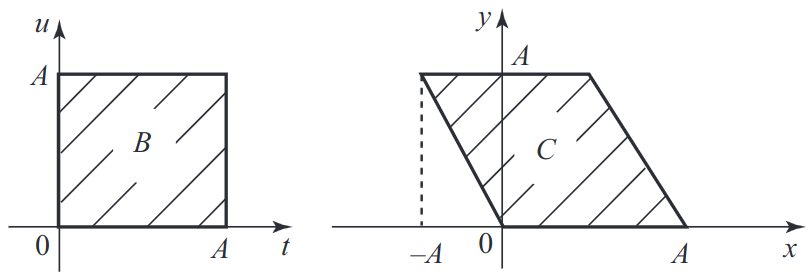
\includegraphics[width = \linewidth]{smd_jv_pic_1.png}
    \end{center}

    \begin{equation}
        \begin{aligned}
        g(\lambda, A) & = \frac{1}{\sqrt{2 \pi} A}\left[\int\limits_{-A-x}^0 \int\limits_0^A d y R(x) e^{-i \lambda x} d x+\int\limits_0^A \int\limits_0^{A-x} d y R(x) e^{-i \lambda x} d x\right]= \\
        & =\frac{1}{\sqrt{2 \pi} A}\left[\int\limits_{-A}^0(A+x) R(x) e^{-i \lambda x} d x+\int\limits_0^A(A-x) R(x) e^{-i \lambda x} d x\right]= \\
        & =\frac{1}{\sqrt{2 \pi}} \int\limits_{-A}^A\left(1-\frac{|x|}{A}\right) R(x) e^{-i \lambda x} d x=\frac{1}{\sqrt{2 \pi}} \int\limits_{-\infty}^{\infty} \mu\left(\frac{x}{A}\right) R(x) e^{-i \lambda x} d x ,
        \end{aligned}
    \label{14.13}
    \end{equation}
    
    где
    $$
        \mu(t)=\begin{cases}
        1-|t|, &|t| \leq 1, \\
        0,  &  |t|>1 .
        \end{cases}
    $$
    
   Покажем, что функция $g(\lambda, A)$ интегрируема на всей прямой. 
   
   Рассмотрим интеграл
    $$
    \int\limits_{-\infty}^{\infty} \mu\left(\frac{\lambda}{2 M}\right) g(\lambda, A) d \lambda
    =\frac{1}{\sqrt{2 \pi}} \int\limits_{-\infty}^{\infty} \mu\left(\frac{x}{A}\right) R(x) \int\limits_{-\infty}^{\infty} \mu\left(\frac{\lambda}{2 M}\right) e^{-i \lambda x} d \lambda d x .
    $$
    
 Поскольку
    $$
    \begin{aligned}
    & \int\limits_{-\infty}^{\infty} \mu\left(\frac{\lambda}{2 M}\right) e^{-i \lambda x} d \lambda=\int_{-2 M}^{2 M}\left(1-\frac{|\lambda|}{2 M}\right) e^{-i \lambda x} d \lambda= \\
    & =  2 \int_0^{2 M}\left(1-\frac{\lambda}{2 M}\right) \cos (\lambda x) d \lambda=2 \int_0^{2 M}\left(1-\frac{\lambda}{2 M}\right) \frac{d \sin (\lambda x)}{x}= \\
    & =\left.2\left(1-\frac{\lambda}{2 M}\right) \frac{\sin (\lambda x)}{x}\right|_0 ^{2 M}+\frac{1}{M x} \int_0^{2 M} \sin (\lambda x) d \lambda= \\
    & =-\left.\frac{\cos (\lambda x)}{M x^2}\right|_0 ^{2 M}=\frac{1-\cos (2 M x)}{M x^2}=\frac{2 \sin ^2(M x)}{M x^2},
    \end{aligned}
    $$
 
    то с учетом (\ref{14.7}) получаем
    $$
    \begin{aligned}
    & \left|\int\limits_{-\infty}^{\infty} \mu\left(\frac{\lambda}{2 M}\right) g(\lambda, A) d \lambda\right|=\left|M \sqrt{\frac{2}{\pi}} \int\limits_{-\infty}^{\infty} \mu\left(\frac{x}{A}\right) R(x) \frac{\sin ^2(M x)}{(M x)^2} d x\right| \leq \\
    & \leq R(0) \sqrt{\frac{2}{\pi}} \int\limits_{-\infty}^{\infty} \frac{\sin ^2(M x)}{(M x)^2} d(M x)=R(0) .
    \end{aligned}
    $$
    
    Таким образом, функция $g(\lambda, A)$ интегрируема на всей прямой и, как следует из (\ref{14.13}), является обратным преобразованием Фурье для функции $\mu\left(\frac{x}{A}\right) R(x)$. 
   \newline Тогда из свойств преобразований Фурье получается, что в этом случае существует прямое преобразование Фурье
    \begin{equation}
        \mu\left(\frac{x}{A}\right) R(x)=\int\limits_{-\infty}^{+\infty} g(\lambda, A) e^{i \lambda x} d \lambda .
    \label{14.14}
    \end{equation}

    $$
    R(0)=\int\limits_{-\infty}^{+\infty} g(\lambda, A) d \lambda .
    $$
    Учитывая условие нормировки, получаем, что функция $\frac{g(\lambda, A)}{R(0)}$ является плотностью распределения вероятностей некоторой случайной величины.
    
    Из (\ref{14.14}) следует, что $\mu\left(\frac{x}{A}\right) \frac{R(x)}{R(0)}$ является характеристической функцией $\forall A$.
    $$
        \mu\left(\frac{x}{A}\right) \frac{R(x)}{R(0)} 
        \xrightarrow[A \rightarrow \infty]{} \frac{R(x)}{R(0)}.
    $$    
    Поэтому $\frac{R(x)}{R(0)}$ также является характеристической функцией.
    Из теоремы об обращении характеристической функции следует, что существует неубывающая функция $F_1(\lambda)$ ограниченной вариации такая, что
    $$
    \frac{R(x)}{R(0)}=\int\limits_{-\infty}^{+\infty} e^{i \lambda x} d F_1(\lambda).
    $$
    Из последней формулы получаем выражение (\ref{14.11}).
    \end{proof}

    \subsubsection{Следствие из теоремы Бохнера}

    Если $R(t)$ - корреляционная функция стационарного случайного процесса $\xi(t)$, то справедливо выражение (\ref{14.11}). При этом $F(\lambda)$ называется \textbf{спектральной функцией процесса} $\xi(t)$. Если функция $F(\lambda)$ дифференцируема, то $f(\lambda)=F^{\prime}(\lambda)$ называется \textbf{спектральной плотностью процесса} $\xi(t)$,
    
    \begin{equation}
        f(\lambda)=\frac{1}{2 \pi} \int\limits_{-\infty}^{+\infty} e^{-i \lambda t} R(t) d t ,
        \label{14.15}
    \end{equation}
    $$
    F(\lambda)=\int\limits_{-\infty}^\lambda f(u) d u .
    $$
    Если $R(t)-$ вещественная функция, то
    $$
    \begin{aligned}
    & R(t)=\int\limits_{-\infty}^{+\infty} \cos (\lambda t) f(\lambda) d \lambda , \\
    & f(\lambda)=\frac{1}{2 \pi} \int\limits_{-\infty}^{+\infty} \cos (\lambda t) R(t) d t .
    \end{aligned}
    $$

    \subsubsection{Пример}
    Найдем спектральную плотность процесса с корреляционной функцией
    $$
    R(t)=\sigma^2 e^{-\alpha|t|}, \ \  \alpha>0 .
    $$
    
    Используя формулу (\ref{14.15}), получаем
    $$
    \begin{aligned}
    f(\lambda) & = \frac{1}{2 \pi} \int\limits_{-\infty}^{+\infty} e^{-i \lambda t} \sigma^2 e^{-\alpha|t|} d t =  \frac{\sigma^2}{2 \pi} \int\limits_{-\infty}^0 e^{-i \lambda t+\alpha t} d t+\frac{\sigma^2}{2 \pi} \int\limits_0^{+\infty} e^{-i \lambda t-\alpha t} d t= \\
    & =  \frac{\sigma^2}{2 \pi}\left(\frac{1}{\alpha-i \lambda}+\frac{1}{\alpha+i \lambda}\right)=\frac{\sigma^2}{\pi} \cdot \frac{\alpha}{\alpha^2+\lambda^2} .
    \end{aligned}
    $$
   



\newpage
% Теорема Герглотца

\section{Теорема Герглотца}

\textbf{Автор:} Павлова Ирина Денисовна, Б-01-001

\subsection{Введение}

Случайная последовательность $\xi = (\xi_1, \xi_2, ...)$ называется стационарной в \textit{узком смысле}, если для любого множества $B \in \mathcal{B}(R^{\infty})$ и любого $n \geq 1$
\begin{equation}\label{eq1} 
    P \{ (\xi_1, \xi_2, ..) \in B\} = P\{(\xi_{n+1}, \xi_{n+2}, ...) \in B\}.
\end{equation}
Отсюда, в частности, вытекает, что если $\mathbf{E}\xi_1^2 < \infty,$ то  $\mathbf{E}\xi_n$ не зависит от $n$:
\begin{equation}\label{eq2} 
    \mathbf{E}\xi_n = \mathbf{E}\xi_1,
\end{equation}

а ковариация $\mathbf{cov}(\xi_{n+m}, \xi_n) = \mathbf{E}(\xi_{n+m} - \mathbf{E}\xi_{n+m})(\xi_n - \mathbf{E}\xi_n)$ зависит лишь от $m$:

\begin{equation}\label{eq3} 
    \mathbf{cov}(\xi_{n+m}, \xi_n) = \mathbf{cov}(\xi_{1+m}, \xi_1).
\end{equation}

В теореме ниже будут использоваться так называемые стационарные в \textit{широком смысле} последовательности (с конечным вторым моментом), для которых условие \ref{eq1} заменяется условиями \ref{eq2} и \ref{eq3}.

\begin{definition}
    Пусть $\mathcal{B}(R)$ --- наименьшая $\sigma$-алгебра $\sigma(\mathcal{A})$, содержащая систему $\mathcal{A}$. Эта $\sigma$-алгебра называется \textit{борелевской} алгеброй множеств числовой прямой, а ее множества - \textit{борелевскими}.
\end{definition}


\begin{definition}
Последовательность комплекснозначных случайных величин $\xi = (\xi_n)_{n \in \textbf{Z}}$ с $\textbf{E}|\xi_n|^2 < \infty, n \in \textbf{Z}$, называется \textit{стационарной} (в широком смысле), если для всех $n \in \textbf{Z}$

$$\textbf{E}\xi_n = \textbf{E}\xi_0,$$
\begin{equation}\label{eq4}
    \textbf{cov}(\xi_{n+k}, \xi_k) = \textbf{E}(\xi_n, \xi_0), \quad k \in \textbf{Z}
\end{equation}


В дальнейшем будем предполагать $\textbf{E}\xi_{0} = 0$. 


Обозначим 
\begin{equation}\label{eq5} 
    R(n)=\textbf{cov}(\xi_n, \xi_0), \quad n \in \textbf{Z},
\end{equation}
и (в предположении $R(0) = \textbf{E}|\xi_0|^2 \neq 0$)
\begin{equation}\label{eq6} 
    \rho (n) = \frac{R(n)}{R(0)}, \quad n \in \textbf{Z}.
\end{equation}


Функцию $R(n)$ будем называть ковариационной функцией, a $\rho(n)$ –– \textit{корреляционной функцией} (стационарной в широком смысле) последовательности $\xi$.

Непосредственно из определения \ref{eq5} следует, что ковариационная функция $R(n)$ является \textit{неотрицательно определенной} т.е. для любых комплексных чисел $a_1, ..., a_m$ и любых $t_1, ..., t_m \in \textbf{Z}, m \geq 1,$

\begin{equation}\label{eq7}
    \sum\limits_{i, j = 1}^{m} a_i \overline{a_j} R(t_i-t_j) \geq 0
\end{equation}

%В свою очередь отсюда (или непосредственно из \ref{eq5}) нетрудно вывести следующие свойства ковариационной функции:
% Свойства ковариационной функции:
% \begin{eqnarray}\label{8}
%     \begin{gathered}
%         R(0) \geq 0, \quad R(-n) = \overline{R(n)}, \quad |R(n)| \leq R(0), \\
%         |R(n)-R(m)|^2 \leq 2R(0)[R(0)- Re R(n-m)].
%     \end{gathered}
% \end{eqnarray}


\end{definition}

\begin{definition}
    Семейство вероятностных мер $\mathcal{P} = \{ \mathbf{P_{\alpha}}; \alpha \in \mathcal{U} \}$ назовем \textit{относительно компактным}, если любая последовательность мер из $\mathcal{P}$ содержит подпоследовательность,слабо сходящуюся к некоторой вероятностной мере.
\end{definition}

\begin{definition}
    Семейство вероятностных мер $\mathcal{P} = \{ \mathbf{P_{\alpha}; \alpha \in \mathcal{U} }\}$ называется плотным, если для каждого $\varepsilon > 0$ можно показать такой компакт $K \subseteq E$ такой, что 
    $$ \underset{\alpha \in \mathcal{U}}{sup} \mathbf{P_{\alpha}} (E \setminus K ) 	\leq \varepsilon.$$
\end{definition}

\begin{definition}
    Семейство функций распределения $\mathcal{F} = \{ F_{\alpha} ; \alpha \in \mathcal{U} \}$, определенных на $R^n, n \geq 1$, называется \textit{относительно компактным (плотным)}, если таковым является соответствующее семейство вероятностных мер $\mathcal{P} = \{ \mathbf{P_{\alpha}; \alpha \in \mathcal{U}} \}$, где $P_{\alpha}$ --- мера, построенная по $\mathbf{F_{\alpha}}$.
\end{definition}

\begin{theorem}[Герглотц]
Пусть $R(n)$ –– ковариационная функция
стационарной (в широком смысле) случайной последовательности
с нулевым средним. Тогда на $([-\pi, \pi), \mathcal{B}([ -\pi, \pi)))$ найдется такая конечная мера $F=F(B), B \in \mathcal{B}([ -\pi, \pi))$, что для любого $n \in \mathbf{Z}$
\begin{equation}\label{eq9} 
    R(n)= \int\limits_{-\pi}^{\pi} e^{i\lambda n} F(d \lambda),
\end{equation}
где интеграл $\int\limits_{-\pi}^{\pi} e^{i\lambda n} F(d \lambda)$ понимается как интеграл Лебега-Стилтьеса по множеству $[-\pi, \pi)$.
\end{theorem}

\begin{proof}
Положим для $N \geq 1 $ и $\lambda \in [-\pi, \pi]$
\begin{equation}\label{eq10} 
    f_N (\lambda) = \frac{1}{2\pi N} \sum_{k=1}^{N} \sum_{l=1}^{N} R(k-l) e^{-i k \lambda} e^{i l \lambda}.
\end{equation}
В силу неотрицательной определенности $R(n)$ функция $f_N(\lambda)$ неотрицательна. Поскольку число тех пар $(k, l),$ для которых $k-l=m,$ есть $N-|m|,$ то
\begin{equation}\label{eq11} 
    f_N (\lambda) = \frac{1}{2\pi} \sum_{|m| < N} \Big( 1-\frac{|m|}{N} \Big) R(m) e^{-i m \lambda}.
\end{equation}

Пусть 
$$f_N=\int\limits_{B} f_N(\lambda)d\lambda, B \in \mathcal{B}([ -\pi, \pi)).$$
Тогда 
\begin{equation}\label{eq12} 
    \int\limits_{-\pi}^{\pi} e^{i\lambda n} F_N(d\lambda) = \int\limits_{-\pi}^{\pi} e^{i \lambda n}f_N(\lambda)d\lambda = 
    \begin{cases}
        \Big( 1 - \frac{|n|}{N}\Big) R(n),  & |n| < N, \\
        0, & |n| \geq N.
    \end{cases}
\end{equation}


Меры $F_N, N \geq 1,$ сосредоточены на интервале $[-\pi, \pi]$ и $F_N ([-\pi, \pi]) = R(0) < \infty$ для любого $N \geq 1.$ Следовательно, семейство мер $\{F_N\}, N \geq 1, $ плотно, и по теореме Прохорова (теорема 1 \textsection 2 гл.  \RomanNumeralCaps{3}) существуют подпоследовательность $\{N_k\} \subseteq $ и мера $F$ такие, что $F_{N_k} \stackrel{\omega}{\longrightarrow} F.$ (Понятия плотности, относительной компактности, слабой сходимости и теорема Прохорова очевидным образом с вероятностных мер переносятся на любые коечные меры.)


Тогда из \ref{eq12} следует, что 
$$\int\limits_{-\pi}^{\pi} e^{i\lambda n} F(d \lambda) = \lim_{N_k\to\infty} \int\limits_{-\pi}^{\pi} e^{i\lambda n} F_{N_{k}} (d\lambda) = R(n).$$
Построенная мера $F$ сосредоточена на интервале $[-\pi, \pi].$ Не изменяя интеграла $\int\limits_{-\pi}^{\pi} e^{i \lambda n} F (d\lambda),$ можно \textit{переопределить} меру $F$, перенеся <<массу>> $F(\{\pi\}),$ сосредоточенную в точке $\pi,$ в точку $-\pi.$ Так полученная новая мера (обозначим ее снова через $F$) будет уже сосредоточенной на интервале $[-\pi, \pi).$
\end{proof}


\begin{remark}
Меру $F = F(B),$ участвующую в представлении \ref{eq9}, называют \textit{спектральной мерой}, а функцию $F(\lambda)=F([-\pi, \lambda])$ - \textit{спектральной функцией} стационарной последовательности с ковариационной функцией $R(n).$
\end{remark}

\begin{remark}
Спектральная мера $F$ \textit{однозначно} определяется по ковариационной функции. В самом деле, пусть $F_1$ и $F_2$ --- две спектральные меры и 
$$\int\limits_{-\pi}^{\pi} e^{i \lambda n} F_1(d \lambda) = \int\limits_{-\pi}^{\pi} e^{i \lambda n} F_2(d \lambda), \quad n \in \mathbf{Z}.$$

Поскольку любая ограниченная непрерывная функция $g(\lambda)$ может быть равномерно приближена на $[-\pi, \pi)$ тригонометрическими полиномами, то 
$$\int\limits_{-\pi}^{\pi} g(\lambda)F_1(d\lambda) = \int\limits_{-\pi}^{\pi} g(\lambda)F_2(d\lambda),$$
откуда следует, что $F_1(B) = F_2(B)$ для любых $B \in \mathcal{B}([-\pi, \pi)).$
\end{remark}
\begin{remark}
Если $\xi = (\xi_n)$ --- стационарная последовательность, состоящая из \textit{действительных} случайных величин $\xi_n$, то $R(n)=R(-n)$ и поэтому
$$R(n)= \frac{R(n) + R(-n)}{2} = \int\limits_{-\pi}^{\pi} \cos \lambda n F(d\lambda).$$

\end{remark}

\begin{theorem}[Прохорова]
    Пусть $\wp = \{ \mathbf{P}_\alpha; \alpha \in  \mathcal{U} \}$ --- семейство вероятностных мер, заданных на полном сепарабельном метрическом пространстве $(E, \xi, \rho)$. Семейство $\wp$ является относительно компактным тогда и только тогда, когда оно является плотным.
\end{theorem}



\newpage
% Стационарный белый шум с непрерывным временем


\section{Стационарный белый шум с непрерывным временем}

\textbf{Автор:} Роман Соколов, Б-01-005

\subsection{Обобщённые стационарные случайные процессы}

\paragraph{Напоминание.}
Обобщённая функция -- непрерывный линейный функционал, определённый на некотором пространстве основных функций. 
Рассмотрим пространство основных функций S. Оно состоит из бесконечно дифференцируемых функций $\phi(t)$, убывающих на бесконечности быстрее любой степени вместе с их производными:
$$\forall m \geq 0 \mapsto (1 + |t|^m)\phi^{(k)}(t) \longrightarrow 0, k = 0, 1, ...$$
\paragraph{Определение. } Обобщёнными случайным процессом $\xi = \xi(\phi)$ будем называть непрерывное линейное отображение $\xi:\phi \longrightarrow L_{\Omega}^2$ множества основных функций $\phi$ в множество случайных величин $L_{\Omega}^2$, где $L^2_{\Omega}$ -- гильбертово пространство случайных величин, суммируемых с квадратом.

Если $\xi(t)$ -- обычный случайный процесс с кореляционной функцией B(s, t), (при $T = (-\infty, +\infty)$ возникает и отображение  $\xi \longrightarrow \xi(\phi)$, т.е. обобщённый случайный процесс.

Получить обобщённые случайные процессы, не сводящиеся к обыкновенным, можно, например, операцией дифференцирования. Обобщённый случайный процесс можно дифференцировать сколь угодно раз, пользуясь определением $$(\xi', \phi) = -(\xi, \phi').$$ После того как обыкновенный процесс продиффернцировали столько раз, сколько позволяет гладкость корреляционной функции, дальнейшие производные будут обощёнными процессами.

\paragraph{Определения. } 
\begin{enumerate}
    \item Математическое ожидание
$$m(\phi) = \textbf{M}\xi(\phi)$$
(это линейный, в силу линейности $\xi (\phi)$ функционал)
    \item Корреляционный функционал
$$B(\phi, \psi) = \textbf{M}\xi(\phi)\overline{\xi(\psi)}$$
(это билинейный эрмитов функционал: $B(\phi, \psi) = \overline{B(\phi, \psi)}$
    \item Обобщённый стационарный процесс -- это отображение  $\xi:\phi \longrightarrow L_{\Omega}^2$ пространства $S = {\phi}$ основных функций в $L_{\Omega}^2$, для которого
    $$\textbf{M}\xi(\phi) = m \int_{-\infty} ^ {+\infty}\phi(t)dt, m - \text{число}$$
    $$\textbf{M}|\xi(\phi)|^2 = (B, \phi * \overline{\phi(-t)})$$
\end{enumerate}

\subsection{Винеровский процесс}
Как известно, броуновским движением называется наблюдаемое под микроскопом движение мелких частиц, взвешенных в жидкости. Построим его математическую модель. Пусть $\omega(t)$ -- абсцисса движущейся точки в момен $t, t \geq 0$. Для простоты $\omega(0) = 0$. Броуновская частица ведёт себя столь нерегулярно, что для любых значений $t_1 < t_2 < ... < t_n$ приращения процесса $\omega(t)$, т.е. разности
$$\omega(t_1) - \omega(t_0) = \omega(t_1), ..., \omega(t_n) - \omega(t_{n - 1}),$$ естественно считать независимыми случайными величинами. Предположим дополнительно, что распределение любой из разностей $\omega(t_{i + 1}) - \omega(t_{i})$ нормально с нулевым математическим ожиданием и дисперсией $\sigma^2(t_{i + 1} - t_{i})$, где $\sigma$ - некоторый параметр. Этим предположением задаётся совместное рапределение разностей: как распределение независимых случайных величин. Следовательно, задаётся и распределение величин
$$\omega(t_1), ..., \omega(t_n)$$
как функций от величин разностей, т.е. конечномерное распределение процесса $\omega(t)$. Случайный процесс с такими конечномерными распределениями называется винеровским процессом. 

\subsection{Белый шум}
Построим с помощью винеровского процесса случайную меру с ортогональными значениями.

Выпустим из точки $\omega(0) = 0$ две независимые реализации винеровского процесса $\omega_1(t)$ и $\omega_2(t)$, $t \geq 0$. На оси значений $\lambda: -\infty < \lambda < \infty$ введём функцию $Z(\lambda)$ по следующему правилу: $Z(0) = 0$, для $\lambda > 0$
положим $Z(\lambda) = \omega_1(\lambda)$, а для $\lambda < 0$
положим $Z(\lambda) = -\omega_2(-\lambda) = -\omega_2(|\lambda|)$. Для отрезка $[\lambda_1, \lambda_2], \lambda_1 < \lambda_2$ положим
$$Z\{[\lambda_1, \lambda_2]\} = Z(\lambda_2) - Z(\lambda_1)$$
(для $0 \leq \lambda_1 < \lambda_2$ случайная мера $Z\{[\lambda_1, \lambda_2]\} = \omega_1(\lambda_2) - \omega_1{\lambda_1}$);
для $\lambda_1 < \lambda_1 \leq 0$ случайная мера $Z\{[\lambda_1, \lambda_2]\} = \omega_2(|\lambda_1|) - \omega_2(|\lambda_2|)$, а если $\lambda_1 < 0 < \lambda_2$, то мера $Z\{[\lambda_1, \lambda_2]\}$ равна сумме мер отрезков $[\lambda_1, 0]$ и $[0, \lambda_2]$). При этом $\textbf{M}|Z\{[\lambda_1, \lambda_2]\}|^2 = \sigma^2|\lambda_1 - \lambda_2|$, $\textbf{M}Z\{[\lambda_1, \lambda_2]\}$ = 0, а для непересекающихся отрезков $[\lambda_1, \lambda_2]$ и $[\lambda_1', \lambda_2']$ значения меры $Z$ независимы, следовательно, и ортогональны.

Можно продолжить меру Z на борелевские подмножества A, получив, что 
$$F(A) = \textbf{M}|Z(A)|^2 = \sigma^2 l(A),$$ $l(A)$ - лебегова мера (длина A). Мера F(A) есть мера степенного роста: 
$$\int_{-\infty}^{+\infty}\frac{F(d\lambda)}{1 + \lambda ^ 3} = \int_{-\infty}^{+\infty}\frac{\sigma^2(d\lambda)}{1 + \lambda ^ 3} < \infty$$

Следовательно можно рассмотреть обобщённый случайный процесс $\xi$ со спектральной мерой Z. Этот процесс называется белым шумом интенсивности $\sigma^2$. Его корреляционный функционал B является преобразованием Фурье от меры $\sigma ^2l(A)$, т.е. равен $2\pi \sigma^2 \delta(t)$. Следовательно $$\textbf{M}|\xi(\phi)| ^ 2 = (B, \phi * \overline{\phi(-t)}) = 2\pi\sigma^2 \int_{-\infty}^{+\infty} |\phi(t)|^2 dt = 2\pi\sigma^2||\phi||^2,$$ где $||\phi||^2$ понимается в смысле нормы в $L^2$ по мере Лебега.

Если на всей прямой $-\infty < t < \infty$ определить винеровский процесс $\omega(t)$ (так же, как это было сделано для функции $Z(\lambda)$) c параметром $2\pi\sigma^2$, то случайный процесс $\xi(t)$ можно понимать как обобщённую производную $\omega(t)$. Действительно, для гладкой финитной функции $\phi = \phi(t)$

\begin{multline*}
  (\omega', \phi) = -(\omega, \phi') = -\int_{-\infty}^{+\infty} \omega(t)\phi'(t)dt = -\int_{-\infty}^{+\infty}\omega(t)d\phi(t) = \\ = -lim \sum_{i}\omega(t_i)(\phi(t_{i+1}) - \phi(t_{i})) = lim \sum_{i}\phi(t_i)(\omega(t_{i}) - \phi(t_{i-1}))  
\end{multline*}
откуда 
$$\textbf{M}|(\omega', \phi)|^2 = 2\pi\sigma^2 lim \sum_{i}|\phi(t_i)|^2 (t_i - t_{i-1}) = 2\pi\sigma^2\int_{-\infty}^{+\infty} |\phi(t)|^2 dt, $$
$$\textbf{M}(\omega', \phi) = 0$$

Итак, белый шум есть обобщённая производная от винеровского процесса. Поскольку приращения винеровского процесса в различные моменты времени независимы, говорят еще, что белый шум есть процесс с независимыми значениями. его спектральная плотность равна константе.

Часто на практике случайный процесс, о котором мало что известно, считают белым шумом. Также пользуются белым шумом в полосе частот $\Lambda$: считают, что $f(\lambda) = C$ при $|\lambda| \leq \Lambda$ и 
$f(\lambda) = 0$ при $|\lambda| > \Lambda$. Нелишне заметить, что белый шум в полосе частот -- это обыкновенный процесс, реализации которого $\xi(t)$ являются аналитическими функциями t. Поэтому не следует абсолютизировать эту модель(как и модель белого шума, значения которго при каждом t бесконечны).


\newpage
% Частотная характеристика линейного преобразования. Формула преобразования спектральной плотности

\section{Частотная характеристика линейного преобразования. Формула преобразования спектральной плотности.}

 \textbf{Автор:} Пузанков Артем Олегович, Б-01-003

\subsection{Стационарные случайные процессы \footnote{Розанов Ю. А. Стационарные случайные процессы., М.: Наука. Гл. ред. физ.-мат. лит., 1990, с. 7-9} }

Пусть $\Omega$ - некоторое измеримое пространство элементов $\omega$ (элементарных событий) с $\sigma$-алгеброй $\mathfrak{A}$ $\omega$-множеств, на которой определена вероятностная мера $P(d\omega)$. Случайной величиной $\xi$ мы будем называть всякую комплексную функцию $\xi(\omega)$ на пространстве $\Omega$, измеримую относительно $\sigma$-алгебры $\mathfrak{A}$. Под случайным процессом $\xi(t)$ будем понимать совокупность случайных величин, зависящих от параметра $t$ (времени), который принимает либо все целые значения, либо все действительные значения (случаи дискретного и непрерывного времени).

\begin{definition} Случайный процесс $\xi(t)$ называется \emph{стационарным в широком смысле}, если его математическое ожидание $M\xi(t)$: $$M\xi(t) = \int_{\Omega}\xi(\omega,t)P(d\omega) = m,$$ есть постоянная, не зависящая от $t$, а \emph{кореляционная функция} $B(t,s)$ (часто обозначают буквой $R$): $$B(t,s) = M\xi(t)\overline{\xi(s)} = B(t-s),$$ зависит лишь от разности $t-s$.
\end{definition}

 \begin{definition} Стационарные в широком смысле случайные процессы $\xi_1(t)$ и $\xi_2(t)$ называются \emph{стационарно связанными}, если их \emph{взаимная корелляционная функция} $$B_{12}(t,s) = M\xi_1(t)\overline{\xi_2(s)} = B_{12}(t-s)$$ зависит лишь от разности $t-s$.
 \end{definition}

\begin{definition}  Совокупность $n$ стационарных процессов $\xi_k(t), \ k = \overline{1,n}$, стационарно связанных между собой, будем называть \emph{n-мерным стационарным процессом} и изображать в виде вектора-столбца $$\xi(t) = \{\xi_k(t)\}_{k=\overline{1,n}}.$$
\end{definition}

Пусть $\xi(t) = \{\xi_k(t)\}_{k=\overline{1,n}}$ - n-мерный стационарный процесс, $H_\xi$ - линейная оболочка величин $\xi_k(t), \ k=\overline{1,n}, \ -\infty<t<\infty$, замкнутая относительно сходимости в среднем квадратичном. Если отождествить между собой величины, отличающиеся друг от друга лишь с вероятностью равной нулю, и ввести скалярное произведение элементов $h', \ h''$ из $H_\xi$, как $$(h',h'') = Mh'\overline{h''},$$ то $H_\xi$ станет гильбертовым пространством; будем называть его \emph{пространством значений} процесса $\xi(t)$.

\subsection{Спектральные представления стационарных процессов \footnote{Розанов Ю. А. Стационарные случайные процессы., М.: Наука. Гл. ред. физ.-мат. лит., 1990, с. 23-27}}

Пусть $\xi(t)=\{\xi_k(t)\}_{k=\overline{1,n}}$ - n-мерный стационарный в широком смысле процесс, $H_\xi$ - пространство его значений.

\begin{lemma}\label{hellopuza_lemma_2.1} Пусть $M$ - некоторое множество в гильбертовом пространстве, на котором задан изометрический оператор $U$ \footnote{Оператор $U$ называется изометрическим, если $$(Uh',Uh'') = (h',h'')$$ для любых $h'$ и $h''$ из $M$.}. Тогда $U$ можно продолжить с сохранением изометричности на $H_M$ - линейное замыкание элементов из $M$.
\end{lemma}


\begin{proof} Покажем сначала, что изометрический оператор $U$ является линейным.

Пусть элемент $h$, 
\begin{equation} 
	\label{h_vid} h = \sum_{k=1}^{m}c_kh_k 
\end{equation} 
принадлежит $M$ вместе с $h_1, h_2, \ldots, h_m$. Тогда $$(Uh,Uh') = (h,h') = \sum_{k=1}^{m}c_k(h_k,h') = \sum_{k=1}^{m}c_k(Uh_k,Uh') = \left(\sum_{k=1}^{m}c_kUh_k,Uh'\right), $$ $$\left(Uh - \sum_{k=1}^{m}c_kUh_k,Uh'\right) = 0$$ для любого элемента $h' \in M$, в частности, для $h' = h, h_1, \ldots, h_m$, и поэтому
\begin{equation}\label{h_rav}
\begin{split}
    & \left(Uh-\sum_{k=1}^{m}c_kUh_k,Uh-\sum_{k=1}^{m}c_kUh_k\right) = 0, \\
    & Uh = \sum_{k=1}^{m}c_kUh_k,
\end{split}
\end{equation}
равенством (\ref{h_rav}) определим теперь оператор $U$ для всех элементов $h$ вида (\ref{h_vid}), где $h_k \in M$.

 Всякий элемент $h$ из $H_m$ является пределом элементов $h_n, \ n = 1, 2, 3, \ldots$, этого вида. Имеем: $$\lim_{n \to \infty} \parallel   h_n - h\parallel   = 0,$$ $$\lim_{m,n \to \infty} \parallel  h_m - h_n\parallel   = \lim_{m,n \to \infty} \parallel  Uh_m - Uh_n\parallel   = 0,$$ и поэтому существует предел $$\lim_{n \to \infty} Uh_n.$$

 Положим 
\begin{equation}
	 \label{h_lim} Uh = \lim_{n \to \infty} Uh_n. 
\end{equation}
Легко проверить, что оператор $U$, определенный равенствами (\ref{h_rav}) и (\ref{h_lim}) на всем пространстве $H_m$, будет изометрическим.
\end{proof}


\begin{theorem}\label{hellopuza_theor_2.1} Каждый многомерный стационарный процесс $\xi(t) = \{\xi_k(t)\}_{k=\overline{1,n}}$ допускает спектральное представление $$\xi(t) = \int e^{i \lambda t} \Phi(d \lambda)$$ в виде интеграла по спектральной случайной мере $\Phi = \{\Phi_k\}_{k=\overline{1,n}}$ (интегрирование производится в пределах $-\pi \leq \lambda \leq \pi$ в случае дискретного времени и в пределах $-\infty < \lambda < \infty$ в случае непрерывного $t$).
\end{theorem}

\subsection{Линейные преобразования стационарных процессов \footnote{Розанов Ю. А. Стационарные случайные процессы., М.: Наука. Гл. ред. физ.-мат. лит., 1990, с. 46-50}}

 Пусть $\xi(t)=\{\xi_k(t)\}_{k=\overline{1,n}}$ - некоторый n-мерный стационарный процесс, спектральное разложение которого 
\begin{equation} 
	\xi(t)=\int e^{i \lambda t} \Phi^\xi(d \lambda), \ \ \Phi^\xi = \{\Phi^\xi_k\}_{k=\overline{1,n}}.
 \end{equation}

 Условимся говорить, что m-мерный стационарный процесс $\eta(t) = \{\eta_j(t)\}_{j=\overline{1,m}}$ получается из $\xi(t)$ \emph{линейным преобразованием}, если каждая его компонента допускает спектральное представление вида 
\begin{equation} 
	\label{lin_pre} \eta_j(t) = \int e^{i \lambda t} \phi_j(\lambda) \Phi^\xi(d \lambda), \ \ j = \overline{1,m}, 
\end{equation} 
с некоторой векторной функцией $\phi_j = \{\phi_{jk}\}^{k=\overline{1,n}}$ из пространства $L^2(F)$.

 Соотношение (\ref{lin_pre}) можно записать в матричной форме: 
\begin{equation} 
	\label{mat_lin_pre} \eta(t) = \int e^{i \lambda t} \phi_{\eta \xi}(\lambda) \Phi^\xi(d \lambda)
\end{equation} 
(здесь матрица $\phi_{\eta \xi}(\lambda) = \{\phi_{jk}(\lambda)\}^{k=\overline{1,n}}_{j=\overline{1,m}}$ символически умножается на матрицу $\Phi^\xi(d \lambda) = \{\Phi^\xi_k(d \lambda)\}_{k=\overline{1,n}}$ состоящую из одного столбца). Формулы (\ref{lin_pre}) и (\ref{mat_lin_pre}) показывают, что случайные величины $\eta_j(t)$ - значения стационарного процесса $\eta(t)$ - принадлежат пространству $H_\xi$.

 Будучи стационарным процессом, $\eta(t)$ имеет свое спектральное представление: 
\begin{equation} 
	\eta(t) = \int e^{i \lambda t} \Phi^\eta(d \lambda), \ \  \Phi^\eta = \{\Phi^\eta_j\}_{j=\overline{1,m}}. 
\end{equation}

 Из соотношения (\ref{lin_pre}) вытекает, что спектральная случайная мера $\Phi^\eta = \{\Phi^\eta_j\}_{j=\overline{1,m}}$ процесса $\eta(t)$ такова, что 
\begin{equation} 
	\label{pre_mera} \Phi^\eta_j(\Delta) = \int_{\Delta} \phi_j(\lambda) \Phi^\xi(d \lambda), \ j=\overline{1,m}
 \end{equation}

 В матричной форме соотношения (\ref{pre_mera}) можно записать как 
\begin{equation} 
	\label{mat_pre_mera} \Phi^\eta(\Delta) = \int_{\Delta} \phi_{\eta\xi}(\lambda) \Phi^\xi(d \lambda). 
\end{equation}

 Компоненты $F^{\eta\eta}_{ij}$ спектральной меры $F^{\eta\eta} = \{F^{\eta\eta}_{ij}\}^{j=\overline{1,m}}_{i=\overline{1,m}}$ процесса $\eta(t)$ выражаются через спектральную меру $F^{\xi\xi} = \{F^{\xi\xi}_{kl}\}^{l=\overline{1,n}}_{k=\overline{1,n}}$ процесса $\xi(t)$ при помощи равенств \begin{equation} 
	F^{\eta\eta}_{\ij}(\Delta) = \int_{\Delta} \phi_i F^{\xi\xi}(d \lambda) \phi^{*}_j, \ \ i,j=\overline{1, m}, 
\end{equation} 
или, в матричной форме, 
\begin{equation} 
	F^{\eta\eta}(\Delta) = \int_{\Delta} \phi_{\eta\xi}F^{\xi\xi}(d \lambda) \phi^{*}_{\eta\xi}. 
\end{equation}

 Будем называть матричную функцию 
\begin{equation} 
	\phi_{\eta\xi} = \{\phi_{jk}\}^{k=\overline{1,n}}_{j=\overline{1,m}} 
\end{equation} 
\emph{спектральной (частотной) характеристикой} нашего линейного преобразования.

 Очевидно, стационарные процессы $\xi(t)$ и $\eta(t)$ стационарно связаны между собой. Пусть их взаимная спектральная мера есть 
\begin{equation} 
	F^{\eta\xi} = \{F^{\eta\xi}_{jk}\}^{k=\overline{1,n}}_{j=\overline{1,m}}. 
\end{equation} 
Имеем
\begin{equation}
\label{spec_mera}
\begin{split}
    & F^{\eta\eta}(d \lambda) = \phi_{\eta\xi}(\lambda)F^{\xi\xi}(d \lambda)\phi^{*}_{\eta\xi}(\lambda), \\
    & F^{\eta\xi}(d \lambda) = \phi_{\eta\xi}(\lambda)F^{\xi\xi}(d \lambda).
\end{split}
\end{equation}

 Соотношения (\ref{spec_mera}) не только необходимы, но и достаточны для того, чтобы многомерный стационарный процесс $\eta(t)$ получался из многомерного стационарного процесса $\xi(t)$ при помощи линейного преобразования со спектральной характеристикой $\phi_{\eta\xi}$.

\begin{lemma}\label{hellopuza_lemma_3.1} Пусть стационарный процесс $\eta(t) = \{\eta_j(t)\}_{j=\overline{1,m}}$ стационарно связан с процессом $\xi(t) = \{\xi_k(t)\}_{k=\overline{1,n}}$, а стационарный процесс $\zeta(t) = \{\zeta_j(t)\}_{j=\overline{1,m}}$ получается из $\xi(t)$ линейным преобразованием, причем их спектральные меры удовлетворяют условиям 
	\begin{equation} 
		\label{spec_usl} F^{\eta\eta}(d \lambda) = F^{\zeta\zeta}(d \lambda), \ \ F^{\eta\xi}(d \lambda) = F^{\zeta\xi}(d \lambda). 
	\end{equation} 
Тогда процессы $\eta(t)$ и $\zeta(t)$ тождественны.
	
\end{lemma}

\begin{proof} Равенства
\begin{equation}
\label{op_T}
\begin{split}
    & T\zeta_j(t) = \eta_j(t), \ j=\overline{1,m}, \\
    & T\xi_k(t) = \xi_k(t), \ k=\overline{1,n}, \ -\infty < t < \infty,
\end{split}
\end{equation}
определяют на элементах $\zeta_i(t)$ и $\xi_k(t)$ пространства $H_\xi$ изометрический оператор $T$: $$M\zeta_j(t)\overline{\zeta_{j'}(t')} = \int e^{i \lambda (t - t')} F^{\zeta\zeta}_{jj'}(d \lambda) = \int e^{i \lambda (t - t')} F^{\eta\eta}_{jj'}(d \lambda) = M \eta_j(t)\overline{\eta_{j'}(t')}$$ и, аналогично, $$M\zeta_j(t)\overline{\xi_k(t')} = M\eta_j(t)\overline{\xi_k(t')}.$$

 По лемме~\ref{hellopuza_lemma_2.1} оператор $T$ можно продолжить с сохранением изометричности на все пространство $H_\xi$. Но в силу равенств (\ref{op_T}) оператор $T$ является тождественным (он переводит случайные величины $\xi_k(t)$ в самих себя), и поэтому $$\zeta_j(t) = \eta_j(t), \ j=\overline{1,m},$$ при всех $t$, что и требовалось доказать.
\end{proof}

\begin{theorem}\label{hellopuza_theor_3.1} Пусть многомерные стационарные процессы $\eta(t)$ и $\xi(t)$ стационарно связаны.

 Для того чтобы процесс $\eta(t)$ получался из $\xi(t)$ линейным преобразованием со спектральной характеристикой $\phi_{\eta\xi}$, необходимо и достаточно, чтобы спектральные меры $F^{\eta\eta}, \ F^{\eta\xi}$ и $F^{\xi\xi}$ этих процессов удовлетворяли условию (\ref{spec_mera}).
\end{theorem}

\begin{proof} Пусть $$\xi(t) = \int e^{i \lambda t} \Phi^\xi(d \lambda).$$ Определим стационарный процесс $\zeta(t)$ равенством 
	\begin{equation} 
		\label{int_zeta} \zeta(t) = \int e^{i \lambda t} \phi_{\eta\xi}(\lambda) \Phi(d \lambda). 
	\end{equation}

 Интеграл в (\ref{int_zeta}) существует, так как существует интеграл $$\int \phi_{\eta\xi}F^{\xi\xi}(d \lambda) \phi^{*}_{\eta\xi} = \int F^{\eta\eta}(d \lambda).$$

 Очевидно, спектральные меры процессов $\zeta(t), \ \eta(t)$ и $\xi(t)$ удовлетворяют условиям (\ref{spec_usl}), откуда по лемме~\ref{hellopuza_lemma_3.1} вытекает, что процесс $\zeta(t)$ на самом деле совпадает с $\eta(t)$. Теорема доказана.
\end{proof}


\begin{remark}\label{hellopuza_remark_1} Стационарный m-мерный процесс $\eta(t)$, стационарно связанный с n-мерным процессом $\xi(t)$, получается из него линейным преобразованием тогда и только тогда, когда при некотором $t_0$ значения $\eta_j(t_0), \ j=\overline{1,m}$, процесса $\eta(t)$ принадлежат пространству $H_\xi$ значений процесса $\xi(t)$; при этом $\eta_j(t) = U_{t-t_0}\eta_j(t_0), \ j=\overline{1,m}$, где $U_t$ - унитарное семейство процессса $\xi(t)$.
\end{remark}

\begin{remark}\label{hellopuza_remark_2} Если стационарный процесс $\xi(t)$ имеет спектральную плотность $f^{\xi\xi}$, то процесс $\eta(t)$, получающийся из $\xi(t)$ линейным преобразованием со спектральной характеристикой $\phi_{\eta\xi}$, также имеет спектральную плотность, причем, как это следует из (\ref{spec_mera}), $$f^{\eta\eta} = \phi_{\eta\xi}f^{\xi\xi}\phi^{*}_{\eta\xi}, \ \ f^{\eta\xi} = \phi_{\eta\xi}f^{\xi\xi}$$ (здесь $f^{\eta\xi}$ - взаимная спектральная плотность).
\end{remark}

\begin{remark}\label{hellopuza_remark_3} Если процесс $\eta(t)$ получается из процесса $\xi(t)$ линейным преобразованием со спектральной характеристикой $\phi_{\eta\xi}$, которая для почти всех $\lambda$ является невырожденной матрицей, то в свою очередь $\xi(t)$ можно получить из $\eta(t)$ линейным преобразованием, причем $$\phi_{\xi\eta} = \phi_{\eta\xi}^{-1}.$$
\end{remark}

\begin{example} Пусть $\xi(t)$ - стационарный процесс с непрерывным временем, $$\xi(t) = \int_{-\infty}^{\infty} e^{i \lambda t} \Phi(d \lambda),$$ спектральная мера $F$ которого удовлевторяет условию $\int_{-\infty}^{\infty} \lambda^2 F(d \lambda) < \infty.$

 Рассмотрим стационарный процесс $\eta(t)$, получающийся из $\xi(t)$ линейным преобразованием со спектральной характеристикой $\phi(\lambda) = i \lambda$, $$\eta(t) = \int_{-\infty}^{\infty} e^{i \lambda t} (i \lambda) \Phi(d \lambda).$$

 Легко заметить, что процесс $\eta(t)$ получается формальным дифференцированием процесса $\xi(t)$ по времени: $$\eta(t) = \frac{d}{dt}\xi(t).$$

 Этому соотношению можно придать строгий смысл. Функция $i \lambda e^{i \lambda t}$ при каждом фиксированном $t$ есть предел в среднем квадратичном функций $\phi_\epsilon(\lambda) = \frac{1}{\epsilon}\left[e^{i \lambda(t+\epsilon)} - e^{i \lambda t}\right]$ при $\epsilon \to 0$, $$\lim_{\epsilon \to 0} \int_{-\infty}^{\infty} \left|i \lambda e^{i \lambda t} - \phi_\epsilon(\lambda) \right|^2 F(d \lambda) = 0,$$ и поэтому $\eta(t)$ есть предел в среднем квадратичном случайных величин $\frac{1}{\epsilon} \left[\xi(t + \epsilon) - \xi(t)\right]$: $$\lim_{\epsilon \to 0} M \left|\eta(t) - \frac{\xi(t + \epsilon) - \xi(t)}{\epsilon}\right|^2 = 0.$$

 Процесс $\eta(t)$ называют производной (в среднем квадратичном) стационарного процесса $\xi(t)$.
\end{example}



\newpage
% Спектральная плотность процесса, удовлетворяющего уравнениям авторегрессии — скользящего среднего (метод формирующих фильтров)


\section{Спектральная плотность процесса, удовлетворяющего уравнениям авторегрессии — скользящего среднего (метод формирующих фильтров)}

\textbf{Автор:} Агафонов Сергей Алексеевич, Б-01-001

\subsection{Спектральное представление ковариационной функции}

\begin{definition} Случайная последовательность $\xi=\left(\xi_1, \xi_2, \ldots\right)$ называется стационарной в узком смысле, если для любого множества $B \in \mathscr{B}\left(R^{\infty}\right)$ и любого $n \geqslant 1$:
\begin{equation}\label{sergey884_eq_1}
\left\{\left(\xi_1, \xi_2, \ldots\right) \in B\right\}=\left\{\left(\xi_{n+1}, \xi_{n+2}, \ldots\right) \in B\right\} . 
\end{equation}
\end{definition}
Отсюда, в частности, вытекает, что если $\xi_1^2<\infty$, то $\xi_n$ не зависит от $n$ :
\begin{equation}\label{sergey884_eq_2}
\xi_n=\xi_1
\end{equation}
а ковариация
$$
\left(\xi_{n+m}, \xi_n\right)=\left(\xi_{n+m}-\xi_{n+m}\right)\left(\xi_n-\xi_n\right) \text { зависит лишь }
$$
oт $m$ :
\begin{equation}\label{sergey884_eq_3}
\left(\xi_{n+m}, \xi_n\right)=\left(\xi_{1+m}, \xi_1\right)
\end{equation}
Здесь будут исследоваться так называемые стационарные в широком смысле последовательности (с конечным вторым моментом), для которых условие (\ref{sergey884_eq_1}) заменяется условиями (\ref{sergey884_eq_2}) и (\ref{sergey884_eq_3}).

Рассматриваемые случайные величины $\xi_n$ будут предполагаться определенными для $n \in \mathbf{Z}=\{0, \pm 1, \ldots\}$ и к тому же комплекснозначными. Последнее предположение не только не усложняет теорию, но и наоборот делает ее более изящной. При этом, разумеется, результаты для действительных случайных величин легко могут быть получены в качестве частного случая из соответствующих результатов для комплексных величин.

Пусть $H^2=H^2(\Omega, \mathscr{F}, \quad$ ) - пространство (комплекснозначных) случайных величин $\xi=\alpha+i \beta, \alpha, \beta \in R$, с $|\xi|^2<\infty$, где $|\xi|^2=\alpha^2+\beta^2$. Если $\xi, \eta \in H^2$, то положим
\begin{equation}\label{sergey884_eq_4}
(\xi, \eta)=\xi \bar{\eta}
\end{equation}
где $\bar{\eta}=\alpha-i \beta-$ комплексно-сопряженная величина к $\eta=\alpha+i \beta$, и
\begin{equation}\label{sergey884_eq_5}
\parallel \xi\parallel =(\xi, \xi)^{1 / 2} .
\end{equation}
\newpage

Қак и для действительных случайных величин, пространство $H^2$  со скалярным произведением $(\xi, \eta)$ и нормой $\parallel \xi\parallel $ является полны. . В соответствии с терминологией функционального анализа пространство $H^2$ называется унитарным (иначе - комплексным) сильбертовым пространством (случайных величин, рассматриваемых на вероятностном пространстве $(\Omega, \mathscr{F}, \quad))$.
Если $\xi, \eta \in H^2$, то их ковариацией назовем величину
\begin{equation}\label{sergey884_eq_6}
(\xi, \eta)=(\xi-\xi) \overline{(\eta-\eta)}
\end{equation}
Из (\ref{sergey884_eq_4}) и (\ref{sergey884_eq_6}) следует, что если $\xi=\eta=0$, то
\begin{equation}\label{sergey884_eq_7}
(\xi, \eta)=(\xi, \eta)
\end{equation}
\begin{definition} Последовательность комплекснозначных случайных величин $\xi=\left(\xi_n\right)_{n \in \mathbf{Z}}$ с $\left|\xi_n\right|^2<\infty, n \in \mathbf{Z}$, называется стационарной (в широком смысле), если для всех $n \in \mathbf{Z}$
\begin{equation}\label{sergey884_eq_8}
\begin{gathered}
\xi_n=\xi_0, \\
\left(\xi_{n+k}, \xi_k\right)=\left(\xi_n, \xi_0\right), \quad k \in \mathbf{Z} .
\end{gathered}
\end{equation}
\end{definition}
Для простоты изложения в дальнейшем будем предполагать $\xi_0=0$. Это предположение не умаляет общности, но в то же самое время дает возможность (согласно (\ref{sergey884_eq_7})), отождествляя ковариацию со скалярным произведением, более просто применять методы и результаты теории гильбертовых пространств.
Обозначим
\begin{equation}\label{sergey884_eq_9}
R(n)=\left(\xi_n, \xi_0\right), \quad n \in \mathbf{Z}
\end{equation}
и (в предположении $R(0)=\left|\xi_0\right|^2 \neq 0$ )
\begin{equation}\label{sergey884_eq_10}
\rho(n)=\frac{R(n)}{R(0)}, \quad n \in \mathbf{Z}
\end{equation}
Функцию $R(n)$ будем называть ковариационной функцией, а $\rho(n)-$ корреляционной функцией (стационарной в широком смысле) последовательности $\xi$.

Непосредственно из определения (\ref{sergey884_eq_7}) следует, что ковариационная функция $R(n)$ является неотрицательно определенной, т. е. для любых комплексных чисел $a_1, \ldots, a_m$ и любых $t_1, \ldots, t_m \in \mathbf{Z}, m \geqslant 1$,
\begin{equation}\label{sergey884_eq_11}
\sum_{i, j=1}^m a_i \bar{a}_j R\left(t_i-t_j\right) \geqslant 0 .
\end{equation}
В свою очередь отсюда (или непосредственно из (\ref{sergey884_eq_9})) нетрудно вывести следующие свойства ковариационной функции:
\begin{equation}\label{sergey884_eq_12}
\begin{gathered}
R(0) \geqslant 0, \quad R(-n)=\overline{R(n)}, \quad|R(n)| \leqslant R(0) \\
|R(n)-R(m)|^2 \leqslant 2 R(0)[R(0)-\operatorname{Re} R(n-m)] .
\end{gathered}
\end{equation}
\newpage
\subsection{Последовательности}
Приведем некоторые примеры стационарных последовательностей $\xi=\left(\xi_n\right)_{n \in \mathbf{Z}}$. (В дальнейшем слова «в широком смысле», а также указание на то, что $n \in \mathbf{Z}$, часто будут опускаться.)\newline

\textbf{Белый шум.}

Пусть $\varepsilon=\left(\varepsilon_n\right)$ - последовательность ортонормированных случайных величин, $\quad \varepsilon_n=0, \quad \varepsilon_i \varepsilon_j=\delta_{i j}$, где $\delta_{i j}-$ символ Кронекера. Понятно, что такая последовательность является стационарной и
$$
R(n)= \begin{cases}1, & n=0 \\ 0, & n \neq 0 .\end{cases}
$$
Отметим, что эта функция $R(n)$ может быть представлена в виде
\begin{equation}\label{sergey884_eq_13}
R(n)=\int_{-\pi}^\pi e^{i \lambda n} d F(\lambda)
\end{equation}
где
\begin{equation}\label{sergey884_eq_14}
F(\lambda)=\int_{-\pi}^\lambda f(\nu) d \nu, \quad f(\lambda)=\frac{1}{2 \pi}, \quad-\pi \leqslant \lambda<\pi .
\end{equation}
Спектор оказался абсолютно непрерывным с постоянной «спектральной» плотностью \\ $f(\lambda) \equiv 1 / 2 \pi$. В этом смысле можно сказать, что последовательность $\varepsilon=\left(\varepsilon_n\right)$ «составлена из гармоник, интенсивность которых одна и та же». Именно это обстоятельство и послужило поводом называть последовательность $\varepsilon=\left(\varepsilon_n\right)$ «белым шумом» по аналогии с («физическим») белым цветом, составленным из различных цветов одной и той же интенсивности.\newline

\textbf{Последовательности скользяцего среднего.}

Отправляясь от белого шума $\varepsilon=\left(\varepsilon_n\right)$, образуем новую последовательность
\begin{equation}\label{sergey884_eq_15}
\xi_n=\sum_{k=-\infty}^{\infty} a_k \varepsilon_{n-k}
\end{equation}
где $a_k$ - комплексные числа такие, что $\sum_{k=-\infty}^{\infty}\left|a_k\right|^2<\infty$.
Из (\ref{sergey884_eq_15}) находим
$$
\left(\xi_{n+m}, \xi_m\right)=\left(\xi_n, \xi_0\right)=\sum_{k=-\infty}^{\infty} a_{n+k} \bar{a}_k
$$
так что $\xi=\left(\xi_k\right)$ является стационарной последовательностью, которую принято называть последовательностью, образованной с помощью (двустороннего) скользящего среднего из последовательности $\varepsilon=\left(\varepsilon_k\right)$.

В том частном случае, когда все $a_k$ с отрицательными индексами равны нулю и, значит,
$$
\xi_n=\sum_{k=0}^{\infty} a_k \varepsilon_{n-k}
$$
последовательность $\xi=\left(\xi_n\right)$ называют последовательностью одностороннего скользящего среднего. Если к тому же все $a_k=0$ при $k>p$, т. е. если
\begin{equation}\label{sergey884_eq_16}
\xi_n=a_0 \varepsilon_n+a_1 \varepsilon_{n-1}+\ldots+a_p \varepsilon_{n-p},
\end{equation}
то $\xi=\left(\xi_n\right)$ называется последовательностью скользящего среднего порядка $р$

Можно показать, что для последовательности (\ref{sergey884_eq_16}) ковариационная функция $R(n)$ имеет вид $R(n)=\int_{-\pi}^\pi e^{i \lambda n} f(\lambda) d \lambda$, где спектральная плотность равна
\begin{equation}\label{sergey884_eq_17}
f(\lambda)=\frac{1}{2 \pi}\left|P\left(e^{-i \lambda}\right)\right|^2
\end{equation}
$\mathrm{c}$
$$
P(z)=a_0+a_1 z+\ldots+a_p z^p
$$\newline

\textbf{Авторегрессионная схема.}

Пусть снова $\varepsilon=\left(\varepsilon_n\right)$ белый шум. Будем говорить, что случайная последовательность $\xi=\left(\xi_n\right)$ подчиняется авторегрессионной схеме порядка $q$, если для $n \in \mathbf{Z}$
\begin{equation}\label{sergey884_eq_18}
\xi_n+b_1 \xi_{n-1}+\ldots+b_q \xi_{n-q}=\varepsilon_n
\end{equation}
При каких условиях на коэффициенты $b_1, \ldots, b_q$ можно утверждать, что уравнение (\ref{sergey884_eq_18}) имеет стационарное решение? Чтобы ответить на этот вопрос, рассмотрим сначала случай $q=1$ :
\begin{equation}\label{sergey884_eq_19}
\xi_n=\alpha \xi_{n-1}+\varepsilon_n
\end{equation}
где $\alpha=-b_1$. Если $|\alpha|<1$, то нетрудно проверить, что стационарная последовательность $\tilde{\xi}=\left(\tilde{\xi}_n\right)$ с
\begin{equation}\label{sergey884_eq_20}
\bar{\xi}_n=\sum_{j=0}^{\infty} \alpha^j \varepsilon_{n-j}
\end{equation}
является решением уравнения (\ref{sergey884_eq_19}). (Ряд в правой части (\ref{sergey884_eq_20}) сходится в среднеквадратическом смысле.) Покажем теперь, что в классе стационарных последовательностей $\xi=\left(\xi_n\right)$ (с конечным вторым моментом) это решение является единственным. В самом деле, из (\ref{sergey884_eq_19}) последовательными итерациями находим, что
$$
\xi_n=\alpha \xi_{n-1}+\varepsilon_n=\alpha\left[\alpha \xi_{n-2}+\varepsilon_{n-1}\right]+\varepsilon_n=\ldots=\alpha^k \xi_{n-k}+\sum_{j=0}^{k-1} \alpha^j \varepsilon_{n-j}
$$

Отсюда следует, что
$$
\left[\xi_n-\sum_{j=0}^{k-1} \alpha^j \varepsilon_{n-j}\right]^2=\left[\alpha^k \xi_{n-k}\right]^2=\alpha^{2 k} \quad \xi_{n-k}^2=\alpha^{2 k} \quad \xi_0^2 \rightarrow 0, \quad k \rightarrow \infty .
$$
Таким образом, при $|\alpha|<1$ стационарное решение уравнения (\ref{sergey884_eq_19}) существует и представляется в виде одностороннего скользящего среднего (\ref{sergey884_eq_20}).
Аналогичный результат имеет место и в случае произвольного $q>1$ : если все нули полинома
\begin{equation}\label{sergey884_eq_21}
Q(z)=1+b_1 z+\ldots+b_q z^q
\end{equation}
лежат вне единичного круга, то уравнение авторегрессии (\ref{sergey884_eq_18}) имеет, и притом единственное, стационарное решение, представимое в виде одностороннего скользящего среднего. При этом ковариационная функция $R(n)$ представима в виде
\begin{equation}\label{sergey884_eq_22}
R(n)=\int_{-\pi}^\pi e^{i \lambda n} d F(\lambda), \quad F(\lambda)=\int_{-\pi}^\lambda f(\nu) d \nu
\end{equation}
где
\begin{equation}\label{sergey884_eq_23}
f(\lambda)=\frac{1}{2 \pi} \cdot \frac{1}{\left|Q\left(e^{-i \lambda}\right)\right|^2}
\end{equation}
В частном случае $q=1$ из (\ref{sergey884_eq_19}) легко находим, что $\xi_0=0$,
$$
\left|\xi_0\right|^2=\frac{1}{1-|\alpha|^2}, \quad R(n)=\frac{\alpha^n}{1-|\alpha|^2}, \quad n \geqslant 0
$$
$(R(n)=\overline{R(-n)}$ для $n<0)$. При этом
$$
f(\lambda)=\frac{1}{2 \pi} \cdot \frac{1}{\left|1-\alpha e^{-i \lambda}\right|^2}
$$

Отсюда следует, что
$$
\left[\xi_n-\sum_{j=0}^{k-1} \alpha^j \varepsilon_{n-j}\right]^2=\left[\alpha^k \xi_{n-k}\right]^2=\alpha^{2 k} \quad \xi_{n-k}^2=\alpha^{2 k} \quad \xi_0^2 \rightarrow 0, \quad k \rightarrow \infty .
$$
Таким образом, при $|\alpha|<1$ стационарное решение уравнения (\ref{sergey884_eq_19}) существует и представляется в виде одностороннего скользящего среднего (\ref{sergey884_eq_20}).
Аналогичный результат имеет место и в случае произвольного $q>1$ : если все нули полинома
$$
Q(z)=1+b_1 z+\ldots+b_q z^q
$$
лежат вне единичного круга, то уравнение авторегрессии (\ref{sergey884_eq_18}) имеет, и притом единственное, стационарное решение, представимое в виде одностороннего скользящего среднего. При этом ковариационная функция $R(n)$ представима в виде
$$
R(n)=\int_{-\pi}^\pi e^{i \lambda n} d F(\lambda), \quad F(\lambda)=\int_{-\pi}^\lambda f(\nu) d \nu
$$
где
$$
f(\lambda)=\frac{1}{2 \pi} \cdot \frac{1}{\left|Q\left(e^{-i \lambda}\right)\right|^2}
$$
В частном случае $q=1$ из (\ref{sergey884_eq_19}) легко находим, что $\xi_0=0$,
$$
\left|\xi_0\right|^2=\frac{1}{1-|\alpha|^2}, \quad R(n)=\frac{\alpha^n}{1-|\alpha|^2}, \quad n \geqslant 0
$$
$(R(n)=\overline{R(-n)}$ для $n<0)$. При этом
$$
f(\lambda)=\frac{1}{2 \pi} \cdot \frac{1}{ \left| 1 - \alpha e^{-i\lambda} \right|^2 } .
$$\newline

\textbf{Смешанная модель авторегрессии и скользящего среднего.}

Если предположить, что в правой части уравнения (\ref{sergey884_eq_18}) вместо $\varepsilon_n$ стоит величина $a_0 \varepsilon_n+a_1 \varepsilon_{n-1}+\ldots+a_p \varepsilon_{n-p}$, то получим так называемую смешанную модель авторегрессии и скользящего среднего порядка $(p, q)$ :
\begin{equation}\label{sergey884_eq_24}
\xi_n+b_1 \xi_{n-1}+\ldots+b_q \xi_{n-q}=a_0 \varepsilon_n+a_1 \varepsilon_{n-1}+\ldots+a_p \varepsilon_{n-p} .
\end{equation}
При тех же предположениях относительно нулей полинома $Q(z)$ далее показывается, что уравнение (\ref{sergey884_eq_24}) имеет стационарное решение $\xi=\left(\xi_n\right)$, для которого ковариационная функция равна $R(n)=\int_{-\pi}^\pi e^{i \lambda n} d F(\lambda)$ с $F(\lambda)=\int_{-\pi}^\lambda f(\nu) d \nu$, где
$$
f(\lambda)=\frac{1}{2 \pi}\left|\frac{P\left(e^{-i \lambda}\right)}{Q\left(e^{-i \lambda}\right)}\right|^2
$$



\newpage
% Прореживание (децимация) стационарного процесса ( Теорема Котельникова)


\section{Прореживание (децимация) стационарного процесса}

\textbf{Автор:} Шамсутдинов Альберт Маратович, Б-01-001	

\subsection{Основные понятия}
\subsubsection{Определение случайного процесса}
\label{sec:def}
Понятие \textsl{случайного процесса} может быть рассмотрено с двух различных, хотя близких по смыслу, сторон.

C одной стороны, пусть $(\Omega, \mathscr{A}, \mathbb{P})$ - некоторое вероятностное пространство, где $\Omega$ - пространство элементарных событий, $\mathscr{A}$ - $\sigma-$алгебра, $\mathbb{P}$ - вероятностная мера, и $T \subseteq  \mathbb{R}$. Будем называть $T$ \textsl{областью определения} процесса. Под \textsl{случайным процессом} $X$ онимают некоторое семейство случайных величин $\{x(t)\}_{t \in T}$, определённых на одном
и том же вероятностном пространстве $(\Omega, \mathscr{A}, \mathbb{P})$. Индексирующий параметр $t \in T$ часто интерпретируют как \textsl{время}. Мы будем рассматривать лишь случайные процессы, принимающие значения в измеримом пространстве $(\mathbb{R}, \mathscr{B}(\mathbb{R}))$, так что  для любого $t \in T$ $x(t):\Omega \to \mathscr{X}$, где $\mathscr{X} \subseteq \mathbb{R}$ - множество возможных значений процесса $X$. Стоит заметить, что случайный процесс является семейством функций двух аргументов: $X = \{x(\omega, t)\}_{\omega \in \Omega, t \in T}$. Аргумент $\omega$ является элементарным событием и принадлежит пространству элементарных событий $\Omega$ с заданной на нем вероятностной мерой. При фиксированном $\omega \in \Omega$ $x(t)$ можно
рассматривать как функцию переменной $t$ называемую \textsl{траекторией} или \textsl{выборочным значением} процесса. Множество всех траекторий называется \textsl{ансамблем}. В каждое время $t_{0}$ и для каждого $\omega_{0} \in \Omega$ у нас имеется число $x(t_{0}, \omega_{0})$. Для
различных $\omega_{i} \in \Omega$ в фиксированный момент времени $t_{0}$ числа $x(t_{0}, \omega_{i})$ представляют собой случайную величину, обозначаемую $X(t_0)$. В конце концов, случайная величина - это не что иное, как присвоение действительных чисел результатам случайного эксперимента. Это очень важное наблюдение и мост, соединяющий концепцию случайного процесса с более привычной концепцией случайной величины. Другими словами, в любой момент времени значение случайного процесса представляет собой случайную величину.


\begin{figure}[b]
\centering
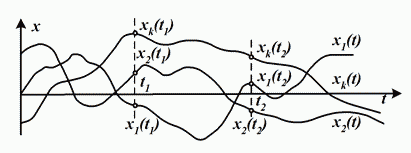
\includegraphics[width=0.8\linewidth]{kekmek1_pic_1.png}
\caption{Реализация случайного процесса $X(t)$}
\label{fig:X}
\end{figure}

Дадим альтернативное определение, рассматривающее случайный процесс как измеримое отображение из вероятностного пространство на пространство траекторий. В такой формулировке процесс выступает в качестве \textsl{случайной функции} от аргумента $t \in T$. Если $T$ — дискретно, то $X$ называют процессом с дискретным временем. Если $T$ — непрерывно, то, соответственно, $X$ называется процессом с непрерывным временем. Этот второй взгляд на случайные процессы, хотя и менее интуитивный, более подходит для точного математического развития теории случайных процессов.
\newpage
\subsubsection{Понятие стационарного процесса}

%\textbf{Определение.} $X$ называется \textsl{стационарным в узком смысле}, если его конечномерные %распределения инвариантны относительно сдвига времени, т.е. для любых $t_1,\dots,t_n \in T$ и $B \in %\mathscr{B(\mathbb{R})}^{n}$:
%{\centering $\mathbb{P}_{t_1,\dots,t_n}(B) = \mathbb{P}_{t_1 + h,\dots,t_n+h}(B)$ \par}

\begin{definition} $X$ называется \textsl{стационарным в широком смысле} процессом, если $\mathbb{E}|X(t)|^{2} < \infty$ для любого $t \in T$ и его среднее и ковариация инвариантны относительно сдвига по времени, т.е. для любых $t, s \in T$:

{\centering 
\begin{equation}
\left\{
    \begin{array}{lr}
        \mathbb{E}(X(t)) = \mathbb{E}(X(t+h)) \\
         Cov(X(t), X(s)) =  Cov(X(t+h), X(s+h))
    \end{array} 
\right.
\end{equation}
}
\end{definition}

\subsubsection{Мощность и энергия}
Благодаря определению случайного процесса, данного в~\ref{sec:def}, мы можем определить понятие мощности и энергии случайного процесса. Пусть $X(t)$-случайный процесс с произвольным выборочным значением $x(t, \omega_{i})$. Тогда энергия и мощность каждой такой функции определено следующим образом:

{\centering 
$$\mathcal{E}_{i} = \int\limits_{-\infty}^{+\infty} x^2(t, \omega_i) dt$$ \\
$$\mathcal{P}_i = \lim\limits_{T\to\infty} \frac{1}{T} \int\limits_{-\frac{T}{2}}^{\frac{T}{2}} x^2(t, \omega_i) dt$$
\par}

Соотношения показывают, что для каждого $\omega_i \in \Omega$ существуют действительные числа 
$\mathcal{E}_i$ и $\mathcal{P}_i$, характеризующий энергию и мощность соответственно. Таким образом, энергия и мощность являются случайными величинами, которые в дальнейшем мы будем обозначать $\mathscr{E}_{X}$ и $\mathscr{P}_{X}$. Имеет смысл определить их математическое ожидание в качестве меры энергии и мощности случайного процесса.

{\centering $P_X = E[\mathscr{P}_X]$ и
$E_X = E[\mathscr{E}_X]$, где \\
$$\mathscr{E}_X = \int\limits_{-\infty}^{+\infty} X^2(t) dt$$ \\
$$\mathscr{P}_X = \lim\limits_{T\to\infty} \frac{1}{T} \int\limits_{-\frac{T}{2}}^{\frac{T}{2}} X^2(t) dt$$
\par}

Из определения следует, 

{\centering
$$E_X = E[\int\limits_{-\infty}^{+\infty} X^2(t) dt] = \int\limits_{-\infty}^{+\infty} E[X^2(t)] dt = \int\limits_{-\infty}^{+\infty} R_x(t, t) dt$$
\par}
{\centering
 и 
}
{\centering
$$P_X = E[\lim\limits_{T\to\infty} \frac{1}{T} \int\limits_{-\frac{T}{2}}^{\frac{T}{2}} X^2(t) dt] = \lim\limits_{T\to\infty} \frac{1}{T} \int\limits_{-\frac{T}{2}}^{\frac{T}{2}} E[X^2(t)] dt = \lim\limits_{T\to\infty} \frac{1}{T} \int\limits_{-\frac{T}{2}}^{+\frac{T}{2}} R_x(t, t) dt$$
\par}   

Если процесс стационарен, то $R_X(t, t) = R_X(0)$ не зависит от времени, если $E_x = \int\limits_{-\infty}^{+\infty} R_x(0) dt < \infty $, то 
$R_X(0) = E[X^2(t)] = 0$. Это значит, что $X(t)$ ноль с вероятность один. Это показывает, что в случае стационарных процессов теоретический и практический интерес представляют только процессы с ненулевой мощностью.

\subsubsection{Случайные процессы в частотной области}
Спектральная плотность мощности случайного процесса является естественным продолжением определения спектральной плотности мощности для детерминированных сигналов, когда также принимается во внимание статистическая природа процесса.

Пусть $X(t)$ - случайный процесс, $x(t, \omega_i)$ произвольная ее реализация.
Усечем функцию $x(t, \omega_i)$ следующим образом:

{\centering 
\begin{equation}
x_T(t, \omega_i)  = 
\left\{
    \begin{array}{lr}
         x(t, \omega_i), |t| < T/2 \\
         0, \ иначе
    \end{array} 
\right.
\end{equation}
}

Так как такая функция является абсолютно интегрируемой с квадратом, то мы можем определить для нее преобразование Фурье. Обозначим преобразование фурье как $X_{T_i} (f)$. Тогда спектральная плотность энергии есть $|X_{T_i} (f)|^2$. Имея спектральную плотность энергии, мы можем
определить спектральную плотность мощности как среднюю спектральную плотность энергии в единицу времени: 
$\frac{|X_{T_i} (f)|^2}{T}$. Теперь, позволив $T$ стать сколь угодно большим, мы определяем спектральную
плотность мощности для рассматриваемой выборочной функции, и мы можем обозначить ее через $\mathcal{S}_{X_i} (f)$. Заметим, что, в общем, различные функции выборки приводят к различным
$\mathcal{S}_{X_i} (f)$. Тогда спектральную плотность мощности случайного процесса можно определить, как

{
\centering
\begin{equation}
    \mathcal{S}_X (f) \equiv E \left[ \lim\limits_{T\to\infty}\frac{|X_{T} (f)|^2}{T} \right] = \lim\limits_{T\to\infty}\frac{E \left[ |X_{T} (f)|^2 \right]}{T}
\end{equation}
}

\subsection{Прореживание стационарного процесса с конечной шириной спектра}

Процесс с конечной шириной спектра - это случайный процесс, спектральная плотность мощности которого занимает
конечную частотную полосу. Другими словами, для такого процесса 
$\mathcal{S}_X (f) \equiv 0$ для любого $f: |f| \geq W $.

\begin{figure}[h]
\centering
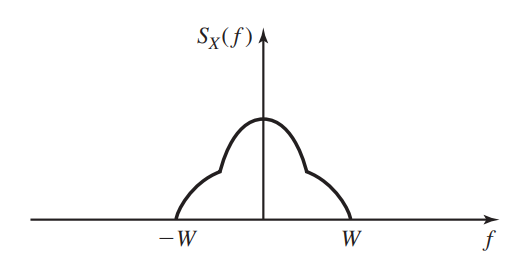
\includegraphics[width=0.8\linewidth]{kekmek1_pic_2.png}
\caption{Ограниченный спектр случайного процесса $X(f)$}
\label{fig:X(f)}
\end{figure}
Типичный пример ограниченного спектра приведен на рис.~\ref{fig:X(f)}.
Теперь мы привели все необходимые понятия, которые необходимы для формулировки следующей теоремы.

\begin{theorem}[Котельникова]
Пусть $X(t)$ стационарный случайный процесс с ограниченным спектром, т.е. $\mathcal{S}_X (f) \equiv 0$ $|f| \geq W $.
Тогда имеет место следующее выражение

{
\centering
\begin{equation}
    E \left| X(t) - \sum\limits_{k=-\infty}^{\infty} X(k T_s) \text{ sinc}(2 W (t-k T_s)) \right| ^ 2 = 0,
\end{equation}
}
где $T_s = \frac{1}{2W}$ определяет интервал прореживания.\\
\end{theorem}
\begin{proof}
Раскроем слагаемое:

\begin{equation*}
	\begin{gathered}
		E \left| X(t) - \sum\limits_{k=-\infty}^{\infty} X(k T_s) \text{ sinc}(2 W (t-k T_s)) \right| ^ 2 = \\
		= R_X(0) - 2\sum\limits_{k=-\infty}^{\infty}R_X(t-k T_s) \text{ sinc}(2 W (t-k T_s)) +\\
		\sum\limits_{k=-\infty}^{\infty}\sum\limits_{l=-\infty}^{\infty} R_X((k-l) T_s)\text{ sinc}(2W(t-k T_s))\text{ sinc}(2W(t-l T_s))
	\end{gathered}
\end{equation*}


В последней строчке приведенного равенства сделаем замену переменных $m = l - k$

{\centering

$\sum\limits_{k=-\infty}^{\infty}\sum\limits_{l=-\infty}^{\infty} R_X((k-l) T_s)\text{ sinc}(2W(t-k T_s))\text{ sinc}(2W(t-l T_s))=$\\
$\sum\limits_{k=-\infty}^{\infty}\sum\limits_{m=-\infty}^{\infty} R_X(-m T_s)\text{ sinc}(2W(t-k T_s))\text{ sinc}(2W(t-k T_s - mT_s)) = $ \\
$\sum\limits_{k=-\infty}^{\infty} \text{ sinc}(2W(t-kT_s)) \sum\limits_{m=-\infty}^{\infty} R_X(mT_s) \text{ sinc}(2W(t-kT_s-mT_s))$
}
Заметим, что последне слагаемое есть разложение в ряд Котельникова функции $R_X(t-kT_s)$, т.е.\\
$\sum\limits_{m=-\infty}^{\infty} R_X(mT_s) \text{ sinc}(2W(t-kT_s-mT_s)) = R_X(t-kT_s)$.

Следовательно, 

{
\centering
$E| X(t) - \sum\limits_{k=-\infty}^{\infty} X(k T_s) \text{ sinc}(2 W (t-k T_s)) | ^ 2 = $\\
$R_X(0) - 2\sum\limits_{k=-\infty}^{\infty}R_X(t-k T_s) \text{ sinc}(2 W (t-k T_s)) +$\\
$\sum\limits_{k=-\infty}^{\infty}R_X(t-k T_s) \text{ sinc}(2 W (t-k T_s))=$\\
$R_X(0) - \sum\limits_{k=-\infty}^{\infty}R_X(t-k T_s) \text{ sinc}(2 W (t-k T_s))$.
}

Нетрудно заметить, что \\ 
$R_X(0) = \sum\limits_{k=-\infty}^{\infty}R_X(t-k T_s) \text{ sinc}(2 W (t-k T_s))$.\\
Следовательно, выполнено необходимое равенство. 

\end{proof}


\newpage
% Стационарная в узком смысле случайная последовательность. Эргодическая теорема Биркгофа—Хинчина.

\section{Стационарная в узком смысле случайная последовательность. Эргодическая теорема Биркгофа—Хинчина}

\textbf{Автор:} Старцев Александр Евгеньевич, Б-01-006

\subsection{Основные понятия}
\subsubsection{Определение стационарной (в узком смысле) случайной последовательности}
\label{sec:def}

Пусть $(\Omega, \mathscr{F}, \mathbb{P})$ - некоторое вероятностное пространство и $\xi = (\xi_1, ~\xi_2, ~...)$ - некоторая последовательность случайных величин, или \textit{случайная последовательность}. Обозначим $\theta_k\xi$ последовательность $(\xi_{k+1}, ~\xi_{k+2}, ~...)$.

\begin{definition} Случайная последовательность $\xi$ называется \textit{стационарной (в узком смысле)}, если для любого $k \geq 1$ распределение вероятностей $\theta_k\xi$ и $\xi$ совпадают:

{\centering 
\begin{equation}
\mathbb{P}\{(\xi_1, ~\xi_2, ~...) \in B\} = \mathbb{P}\{(\xi_{k+1}, ~\xi_{k+2}, ~...) \in B\}, ~~B \in \mathscr{B}(R^{\infty})
\end{equation}
}
\end{definition}

Простейшим примером такой последовательности $\xi$ является последовательность $\xi = (\xi_1, ~\xi_2, ~...)$, состоящяая из \textit{независимых одинаково распределенных} случайных величин. Отправляясь от такой последовательности, можно сконструировать широкий класс стационарных последовательностей $\eta = (\eta_1, ~\eta_2, ~...)$, если взять произвольную борелевскую функцию $g(x_1, ~..., ~x_n)$ и положить $\eta_k = g(\xi_k, ~\xi_{k+1}, ~..., ~\xi_{k+n})$.

\subsubsection{Определение измеримого и сохраняющего меру преобразования}
Пусть $(\Omega, \mathscr{F}, \mathbb{P})$ - некоторое полное вероятностное пространство.

\begin{definition} Отображение $T$ пространства $\Omega$ в себя называется \textit{измеримым}, если для всякого $A \in \mathscr{F}$

{\centering 
\begin{equation}
T^{-1}A = \{\omega: T\omega \in A\} \in \mathscr{F}
\end{equation}
}
\end{definition}

\begin{definition} Измеримое отображение $T$ называется \textit{сохраняющим меру преобразованием} (морфизмом), если для всякого $A \in \mathscr{F}$

{\centering 
\begin{equation}
\mathbb{P}(T^{-1}A) = \mathbb{P}(A)
\end{equation}
}
\end{definition}

Приведем примеры сохраняющих меру преобразований.

\begin{example} Пусть $\Omega = \{\omega_1, ~..., \omega_n\}$ - множество, состоящее из конечного числа точек, $n \geq 2$, $\mathscr{F}$ - все его подмножества, $T\omega_i = \omega_{i+1}$, $1 \leq i \leq n - 1$, и $T\omega_n = \omega_1$. Если $P(\omega_i) = \frac{1}{n}$, то $T$ - сохраняющее меру преобразование.
\end{example}

\begin{example} Если $\Omega = [0, ~1), ~\mathscr{F} = \mathscr{B}([0, 1)), ~\mathbb{P}$ - мера Лебега, $\lambda \in [0, 1)$, то $Tx = (x + \lambda) ~mod ~1$ является сохраняющим меру преобразованием.
\end{example}

Рассмотрим физические предпосылки, приводящие к изучению преобразований, сохраняющих меру.

Будем представлять себе $\Omega$ как фазовое пространство состояний $\omega$ некоторой системы, эволюционирующей (в дискретном времени) в соответствии с заданным законом движения. Тогда, если $\omega$ есть состояние в момент $n = 1$, то $T^n\omega$, где $T$ - оператор сдвига (индуцируемый данным законом движения), есть то состояние, в которое перейдет система через $n$ шагов. Далее, если $A$ - какое-то множество состояний $\omega$, то $T^{-1}A = \{\omega: T\omega \in A\}$ есть по своему определению множество тех "начальных"  состояний $\omega$, которые через один шаг окажутся в множестве $A$. Поэтому, если интерпретировать $\Omega$ как "несжимаемую жидкость", то условие $\mathbb{P}(T^{-1}A) = \mathbb{P}(A)$ можно рассматривать как вполне естественное условие сохранения объема.

\subsubsection{Эргодичность}
Пусть $T$ - \textit{сохраняющее меру} преобразование, действующее на вероятностном пространстве $(\Omega, \mathscr{F}, \mathbb{P})$.

\begin{definition} Множество $A \in \mathscr{F}$ называется \textit{инвариантным}, если $T^{-1}A = A$. Множество $A \in \mathscr{F}$ называется \textit{почти инвариантным}, если $A$ и $T^{-1}A$ отличаются на множетсво меры нуль, т.е. $\mathbb{P}(A \triangle T^{-1}A) = 0$.

Нетрудно проверить, что класс инвариантых (почти инвариантных) множеств образует $\sigma$-алгебру.
\end{definition}

\begin{definition} Сохраняющее меру преобразование $T$ называется \textit{эргодическим} (или \textit{метрически транзитивным}), если каждое инвариантное множество $A$ имееет меру нуль или единица.
\end{definition}

\begin{definition} Случайная величина $\eta = \eta(\omega)$ называется \textit{инвариантной (почти инвариантной)}, если $\eta(\omega) = \eta(T\omega)$ для всех $\omega \in \Omega$ (для почти всех $\omega \in \Omega$).
\end{definition}

Следующая лемма устанавливает свзяь между инвариантными и почти инвариантными множествами.

\begin{lemma} Если $A$ является почти инвариантным множеством, то найдется такое инвариантное множество $B$, что $\mathbb{P}(A \triangle B) = 0$.
\end{lemma}

\begin{proof} Пусть $B = \overline{\rm lim}T^{-n}A$. Тогда \\ $T^{-1}B = \overline{\rm lim}T^{-(n+1)}A = B$, т.е. $B \in \mathscr{J}$. Нетрудно убедиться в том, что $A \triangle B \subseteq \bigcup\limits_{k=0}^{\infty} (T^{-k}A\triangle T^{-(k+1)}A)$. \\ Но $\mathbb{P}(T^{-k}A\triangle T^{-(k+1)}A) = \mathbb{P}(A \triangle T^{-1}A) = 0$. Поэтому $\mathbb{P}(A\triangle B) = \\ = 0$. 
\end{proof}

\begin{lemma} Преобразование $T$ эргодично тогда и только тогда, когда каждое почти инвариантное множество имеет меру нуль или единица.
\end{lemma}

\begin{proof} Пусть $A \in \mathscr{J}^*$. Тогда по лемме 1 найдется инвариантное множество $B$ такое, что $\mathbb{P}(A \triangle B) = 0$. Но $T$ эргодично и, значит, $\mathbb{P}(B) = 0$ или $1$. Обратное очевидно, поскольку $\mathscr{J} \subseteq \mathscr{J}^*$. $\square$
\end{proof}

\begin{theorem} Пусть T - сохраняющее меру преобразование. Следующие условия эквивалентны:
\begin{enumerate}
    \item $T$ эргодично;
    \item каждая почти инвариантная случайная величина есть константа;
    \item каждая инвариантная случайная величина есть константа
\end{enumerate}
\end{theorem}

\begin{proof} $(1) \Rightarrow (2)$. Пусть $T$ эргодично и $\xi$ почти инвариантна, то есть $\xi(\omega) = \xi(T\omega)$. Тогда для любого $c \in R$ множество $A_c = \{\omega: \xi(\omega) \leq c\} \in \mathscr{J}^*$ и по лемме 2 $\mathbb{P}(A_c) = 0$ или $1$. Пусть $C = sup\{c: \mathbb{P}(A_c) = 0\}$. Поскольку $A_c \uparrow \Omega$ при $c \uparrow \infty$ и $A_c \downarrow \varnothing$ при $c \downarrow -\infty$, то $|C| < \infty$. Тогда

{\centering 
$$\mathbb{P}\{\omega: \xi(\omega) < C\} = \mathbb{P}(\bigcup\limits_{k=0}^{\infty} \{\xi(\omega) \leq C - \frac{1}{n}\}) = 0$$ 
\par}

\noindent и аналогично $\mathbb{P}\{\omega: \xi(\omega) > C\} = 0$. Тем самым $\mathbb{P}\{\omega: \xi(\omega) = \\ = C\} = 1$.

$(2) \Rightarrow (3)$. Очевидно

$(3) \Rightarrow (1)$. Пусть $A \in \mathscr{J}$, тогда $I_A$ - нивариантная случайная величина и, значит, $I_A = 0$ или $I_A = 1$, откуда $\mathbb{P}(A) = 0$ или $1$. 
\end{proof}

\begin{remark} Утверждение теоремы остается в силе и в том случае, когда рассматриваемые в ней случайные величины \textit{ограничены}.
\end{remark}

\subsection{Эргодическая теорема Биркгофа и Хинчина}


\begin{theorem}[Биркгоф и Хинчин] Пусть $T$ - сохраняющее меру преобразование и $\xi = \xi(\omega)$ - случайная величина с $\mathbb{E}|\xi| < \infty$. Тогда 

{\centering 
\begin{equation}
\lim_{n\to\infty} \frac{1}{n}\sum_{k=0}^{n-1}\xi(T^{k}\omega) = \mathbb{E}(\xi|\mathscr{J})
\end{equation}
}

Если к тому же $T$ эргодично, то

{\centering 
\begin{equation}
\lim_{n\to\infty} \frac{1}{n}\sum_{k=0}^{n-1}\xi(T^{k}\omega) = \mathbb{E}\xi
\end{equation}
}
\end{theorem}


\begin{lemma}[максимальная эргодическая теорема] Пусть $T$ - сохраняющее меру преобразование, $\xi$ - случайная величина с \\ $\mathbb{E}|\xi| <\infty$ и 

{\centering 
$$S_k(\omega) = \xi(\omega) + \xi(T\omega) + ... + \xi(T^{k-1}\omega)$$ \\
$$M_k(\omega) = \max\{0, ~S_1(\omega), ~..., ~S_k(\omega)\}$$}
\noindent Тогда для любого $n \geq 1$

{\centering 
$$\mathbb{E}[\xi(\omega)I_{\{M_n > 0\}}(\omega)] \geq 0$$}
\end{lemma}

\begin{proof} Если $n > k$, то $M_n(T\omega) \geq S_k(T\omega)$ и, значит, $\xi(\omega) + M_n(T\omega) \geq \xi(\omega) + S_k(T\omega) = S_{k+1}(\omega)$. Так как очевидно, что $\xi(\omega) \geq S_1(\omega) - M_n(T\omega)$, то

{\centering 
$$\xi(\omega) \geq \max\{S_1(\omega), ~..., ~S_n(\omega)\} - M_n(T\omega)$$
\par}

Значит, поскольку $\{M_n(\omega) > 0\} = \{\max(S_1(\omega), ~..., ~S_n(\omega)) > \\ > 0\}$, то

{\centering 
\begin{equation} 
	\begin{gathered}
		\mathbb{E} [ \xi(\omega) I_{\{M_n > 0\}}(\omega)] \geq \mathbb{E}[(\max(S_1(\omega), ~..., ~S_n(\omega)) - M_n(T\omega))I_{\{M_n > 0\}}(\omega)]  \geq \\  \geq \mathbb{E}\{(M_n(\omega) - M_n(T\omega))I_{\{M_n(\omega) > 0\}}\} \geq \mathbb{E}\{M_n(\omega) - M_n(T\omega)\} = 0
	\end{gathered}
\end{equation}
}

где мы воспользовались тем, что если $T$ - сохраняющее меру преобразование, то $\mathbb{E}M_n(\omega) = \mathbb{E}M_n(T\omega)$.
\end{proof}

\begin{proof}[Доказательство теоремы] Будем предполагать $\mathbb{E}(\xi|\mathscr{J}) = 0$ (в противном случае от $\xi$ надо перейти к $\xi - \mathbb{E}(\xi|\mathscr{J})$). 

Пусть $\overline{\rm \eta} = \overline{\rm lim}\frac{S_n}{n}$ и $\underline{\eta} = \underline{\rm lim}\frac{S_n}{n}$. Для доказательства достаточно установить, что

{\centering 
$$0 \leq \underline{\eta} \leq \overline{\eta} \leq 0.$$
\par}

Рассмотрим случайную величину $\overline{\eta} = \overline{\eta}(\omega)$. Поскольку $\overline{\eta} = \\ = \overline{\eta}(T\omega)$, то $\overline{\eta}$ инвариантна и, следовательно, для каждого $\varepsilon > \\ > 0$ множество $A_{\varepsilon} = \{\overline{\eta}(\omega) > \varepsilon\}$ также является инвариантным. Введем новую случайную величину

{\centering 
$$\xi^*(\omega) = (\xi(\omega) - \varepsilon)I_{A_{\varepsilon}}(\omega),$$
\par}

и пусть

{\centering 
$$S_k^*(\omega) = \xi^*(\omega) + ... + \xi^*(T^{k-1}\omega), ~M_k^*(\omega) = \max(0, ~S_1^*, ~..., S_k^*).$$
\par}

Тогда, согласно лемме, для любого $n \geq 1$

{\centering 
$$\mathbb{E}[\xi^*I_{\{M_n^* > 0\}}] \geq 0.$$
\par}

Но при $n \rightarrow \infty$

{\centering 
\begin{equation}
	\begin{gathered}
		\{M_n^* > 0\} = \{\max_{1 \leq k \leq n}S_k^* > 0\}\uparrow \{\sup_{ k \geq 1}S_k^* > 0\} = \{\sup_{ k \geq 1}\frac{S_k^*}{k} > 0\} =  \\
		= \{\sup_{ k \geq 1}\frac{S_k}{k} > \varepsilon\} \cap A_{\varepsilon} = A_{\varepsilon},
	\end{gathered}
\end{equation}
\par}

где последнее равенство следует из того, что $\sup_{ k \geq 1}\frac{S_k}{k} \geq \overline{\eta}$, а $A_{\varepsilon} = \{\omega: \overline{\eta} > \varepsilon\}$.

Далее, $\mathbb{E}|\xi^*| \leq \mathbb{E}|\xi| + \varepsilon$. Поэтому по теореме о мажорируемой сходимости

{\centering 
$$0 \leq \mathbb{E}[\xi^*I_{\{M_n^* > 0\}}] \rightarrow \mathbb{E}[\xi^*I_{A_{\varepsilon}}].$$
\par}

Итак,

{\centering 
\begin{equation}
	\begin{gathered}
		0 \leq \mathbb{E}[\xi^*I_{A_{\varepsilon}}] = \mathbb{E}[(\xi - \varepsilon)I_{A_{\varepsilon}}] = \mathbb{E}[\xi I_{A_{\varepsilon}}] - \varepsilon\mathbb{P}(A_{\varepsilon}) = \\
		 = \mathbb{E}[\mathbb{E}(\xi|\mathscr{J})I_{A_{\varepsilon}}] - \varepsilon\mathbb{P}(A_{\varepsilon}) = -\varepsilon\mathbb{P}(A_{\varepsilon}),
 	\end{gathered}
\end{equation}
\par}

откуда $\mathbb{P}(A_{\varepsilon}) = 0$ и, значит, $\mathbb{P}\{\overline{\eta} \leq 0\} = 1$.

Аналогично, рассматривая вместо $\xi(\omega)$ величину $-\xi(\omega)$, найдем, что 

{\centering 
$$\overline{\rm lim}(-\frac{S_n}{n}) = -\underline{\rm lim}\frac{S_n}{n} = -\underline{\eta}$$
\par}

и $\mathbb{P}\{-\underline{\eta} \leq 0\} = 1$, то есть $\mathbb{P}\{\underline{\eta} \geq 0\} = 1.$ тем самым $0 \leq \underline{\eta} \leq \overline{\eta} \leq 0$, чо и доказывает первое утверждение теоремы.

Для доказательства второго утверждения достаточно заметить, что поскольку $\mathbb{E}(\xi|\mathscr{J})$ - инвариантная величина, то в эргодическом случае $\mathbb{E}(\xi|\mathscr{J}) = \mathbb{E}\xi$.
\end{proof}

\begin{corollary} Сохраняющее меру преобразование $T$ эргодично в том и только в том случае, когда для любых $A, ~B \in \mathscr{F}$
\end{corollary}

{\centering 
\begin{equation}
\lim_{n\to\infty} \frac{1}{n}\sum_{k=0}^{n-1}\mathbb{P}(A \cap T^{-k}B) = \mathbb{P}(A)\mathbb{P}(B).
\end{equation}
}


\newpage
% Статистическая оценка математического ожидания гауссовсекой стационарной последовательности

\section{Статистическая оценка математического ожидания гауссовской стационарной последовательности}

 \textbf{Автор:} Дуденко Екатерина Игоревна, Б-01-001

\subsection{Гауссовский случайный процесс.}
\begin{definition}(Лекции по случайным процессам А.В. Гасников \cite{GasnikovLectionsRP})
Гауссовский процесс - это процесс, все конечномерные распре-
деления которого нормальные (гауссовские). Это значит, что любой
случайный вектор, составленный из сечений такого процесса, имеет
нормальное распределение.
\end{definition}

Напомним, что случайный вектор $X \in \mathbb{\bf{R}} ^ n$ является гауссовским с
математическим ожиданием $m$ и корреляционной матрицей $R \in \mathbb{\bf{R}} ^{n \times n}$
(обозначается $X \in \mathbb{N}(m, R)$), если его характеристическая функция за-
дается формулой:

\begin{equation*}
    \varphi_X(s)  \stackrel{def}{=} \mathbb{E}e^{i\langle{s,X}\rangle} = exp(i\langle{s,m}\rangle - \frac{1}{2}\langle{s,Rs}\rangle), s \in \mathbb{\bf{R}}^n
\end{equation*}

Если $det R \neq 0$ , то $X$ обладает плотностью распределения:
\begin{equation*}
    p_X(u) = \frac{1}{\sqrt{(2\pi)^n det R}} exp(-\frac{1}{2}\langle{u,R^{-1}u}\rangle), u \in \mathbb{\bf{R}^n}
\end{equation*}

\subsection{Стационарные последовательности.}

\begin{definition}(Ширяев вероятность \cite{ShiryaevVeroyatnost1})
Случайная последовательность $\xi = (\xi_1, \xi_2, ...)$ называется стационарной в узком смысле, если для любого множества $B \in \mathbb{\bf{B}}(\mathbb{\bf{R}}^{\infty})$ и любого $n \geq 1$
\begin{equation}
\mathbf{P}\{(\xi_1, \xi_2, ...) \in B \} = \mathbf{P}\{ (\xi_{n+1}, \xi_{n+2}, ...) \in B \}
\end{equation}
\end{definition}
Отсюда, в частности, вытекает, что если $\mathbf{M}\xi_1^2 < \infty$, то $\mathbf{M}\xi_n$ не зависит от $n$: $\mathbf{M}\xi_n=\mathbf{M}\xi_1$

\begin{definition}(Ширяев вероятность \cite{ShiryaevVeroyatnost1})
Последовательность комплексных случайных величин $\xi = (\xi_n)_{n\in\mathbb{Z}}$ с $\mathbf{M}|\xi_n|^2 < \infty, n\in\mathbb{Z}$, называется стационарной (в широком смысле), если для всех $n \in \mathbb{\bf{Z}}$ 

\begin{equation}
\begin{gathered}
\mathbf{M}\xi_n = \mathbf{M}\xi_0 \\
cov(\xi_{k+n}, \xi_k) = cov(\xi_n, \xi_0), \  k\in\mathbb{\bf{Z}}.
\end{gathered}
\end{equation}

\end{definition}

\begin{theorem}(Лекции по случайным процессам А.В. Гасников \cite{GasnikovLectionsRP}) 
Гауссовский процесс является стационарным в широком смысле тогда и только тогда, когда он является стационарным в узком смысле.
\end{theorem}

\subsection{Спектральное представление стационарных последовательностей.}

Если $\xi = (\xi_n)$ - стационарная последовательность с $\mathbf{M}\xi_n = 0, n \in \mathbb{\bf{Z}},$ то, найдется такая конечная мера $F = F(\delta)$ на, $([-\pi, \pi), \mathscr{B}([-\pi, \pi))),$ что ковариационнная функция $R(n) = cov(\xi_{k+n}, \xi_k)$ допускает спектральное представление
\begin{equation}
R(n) = \int_{-\pi}^{\pi} e^{i\lambda n}F(d\lambda).
\end{equation}
Следующий результат дает соответствующее спектральное представление самой последовательности.
\begin{equation}\label{spkt}
\xi_n = \int_{-\pi}^{\pi} e^{i\lambda n}Z(d\lambda).
\end{equation}

При этом $\mathbf{M}|Z(\delta)|^2 = F(\delta)$.

\begin{theorem}\label{t1}(Ширяев вероятность \cite{ShiryaevVeroyatnost1})
Пусть $\xi = (\xi_n)\, n \in \mathbb{Z}\,$ стационарная последовательность с $\mathbf{M}\xi_n = 0$, ковариационной функцией $R(n) = \int_{-\pi}^{\pi}   e^{i\lambda n}F(d\lambda)$ и спектральным разложением $\xi_n = \int_{-\pi}^{\pi} e^{i\lambda n)Z(d\lambda}$. Тогда:
\begin{equation}\label{eq1}
\frac{1}{n}\sum_{k=0}^{n-1}\xi_k \xrightarrow{L^2}Z(\{ 0\})
\end{equation}
$$
\text{и}
$$
\begin{equation}\label{eq2}
\frac{1}{n}\sum_{k=0}^{n-1} R(k) \xrightarrow{}F(\{ 0\})
\end{equation}
\end{theorem}



\begin{proof} 

В силу (\ref{spkt})


\[	
\frac{1}{n} \sum_{k=0}^{n-1}\xi_k = \int_{-\pi^\pi}\sum_{k=0}^{n-1}e^{ik\lambda}Z(d\lambda) = \int_{-\pi}^{\pi}\varphi_n(\lambda)Z(\lambda), \\
\]
\[
\text{где } \varphi_n(\lambda) = \frac{1}{n}\sum_{k=0}^{n-1}e^{ik\lambda} =
\begin{cases*}
1, \lambda = 0,\\
\frac{1}{n}*\frac{e^{in\lambda} - 1}{e^{i\lambda} - 1}, \lambda \neq 0.
\end{cases*}
\]
$$
\text{Поскольку } |\sin\lambda| \geq \frac{2}{\pi}|\lambda| \text{ для } |\lambda|\leq\frac{\pi}{2}, \text{ то}
$$
$$
 |\varphi_n(\lambda)|= \Bigg|\frac{\sin{\frac{n\lambda}{2}}}{n\sin{\frac{\lambda}{2}}}\Bigg| \leq \frac{\pi}{2}
\Bigg|\frac{\sin{\frac{n\lambda}{2}}}{\frac{n\lambda}{2}}\Bigg| \leq \frac{\pi}{2}.
$$
$$
\text{Далее, } \varphi_n(\lambda) \xrightarrow{L^2} I_{\{0\}}(\lambda), \text{ поэтому } 
$$
$$
\int_{-\pi}^{\pi}\varphi_n(\lambda)Z(d\lambda) \xrightarrow{L^2} \int_{-\pi}^{\pi}  I_{\{0\}}(\lambda) Z(d\lambda) = Z({0}),
$$
$$
\text{что и доказывает (\ref{eq1}). Аналогичным образом доказывается и утверждение (\ref{eq2})}
$$
\end{proof}



\begin{corollary}
Если спектральная функция непрерывна в нуле, т. е. $F(\{0\}) = 0$, то $Z(\{0\}) = 0$ и в силу (\ref{eq1}), (\ref{eq2})
\begin{equation}
\frac{1}{n}\sum_{k=0}^{n-1} R(k) \xrightarrow{}0 \Rightarrow \frac{1}{n}\sum_{k=0}^{n-1}\xi_k(k) \xrightarrow{L^2}0 
\end{equation}
\end{corollary}

\begin{proof} 

Поскольку
\begin{equation*}
\Bigg| \frac{1}{n}\sum_{k=0}^{n-1}R(k)\Bigg|^2 = \Bigg|\mathbf{M}\Big(\frac{1}{n}\sum_{k=0}^{n-1}\xi_k\Big) \xi_0\Bigg|^2 \leq \mathbf{M}|\xi_0|^2\mathbf{M}\Big( \frac{1}{n}\sum_{k=0}^{n-1}\xi_k\Big)^2,
\end{equation*}
То верна и обратная импликация:
\begin{equation*}
\frac{1}{n}\sum_{k=0}^{n-1}\xi_k \xrightarrow{L^2}0 \Rightarrow \frac{1}{n}\sum_{k=0}^{n-1}R(k) \xrightarrow {} 0.
\end{equation*}
Таким образом, условие $\frac{1}{n}\sum_{k=0}^{n-1} R(k) \xrightarrow{}0$ является необходимым и достаточным для сходимости (в среднеквадратичном смысле) средних арифметических $\frac{1}{n}\sum_{k=0}^{n-1}\xi_k(k)$ к нулю. 

\end{proof}


\begin{corollary}
Отсюда следует, что для стационарной в широком смысле последовательности $\xi = (\xi_n)$ такой, что ее математическое ожидание есть $m$ $(\mathbf{M}\xi_0=m)$, то
\begin{equation}
\frac{1}{n}\sum_{k=0}^{n-1} R(k) \xrightarrow{}0 \Leftrightarrow \frac{1}{n}\sum_{k=0}^{n-1}\xi_k(k) \xrightarrow{L^2}m.
\end{equation}
где $R(n) = \mathbf{M}(\xi_n - \mathbf{M}\xi_n)(\xi_0 - \mathbf{M}\xi_0)$.
\end{corollary}

\subsection{Статистическое оценивание.}
Пусть $\xi = (\xi_n)$, $n \in \mathbf{\bf{Z}}$ стационарная в широком смысле случайная последовательность с математическим ожиданием $\mathbf{M}\xi_n = m$ и ковариацией $R(n) = \int_{-\pi}^{\pi} e^{i\lambda n}F(d\lambda)$.

Пусть $x_0, x_1, ..., x_{N-1}$ - полученные в ходе наблюдения случайных величин $\xi_0, \xi_1, ..., \xi_{N-1}$. По ним нужно построить 'хорошую' оценку (неизвестного) среднего значения $m$.

Положим
\begin{equation}
m_N(X) = \frac{1}{N}\sum_{k=0}^{N-1}x_k.
\end{equation}

Тогда из элементарных свойств математического ожидания следует, что эта оценка является 'хорошей' оценкой величины $m$ в том смысле, что 'в среднем по всем реализациям $x_0, ..., x_{N-1}$'  она является $несмещенной$, т. е

\begin{equation}
\mathbf{M}m_N(\xi) = \mathbf{M}(\frac{1}{N}\sum_{k=0}^{N-1}\xi_k) = m.
\end{equation}

Более того из теоремы \ref{t1} вытекает, что при условии $\frac{1}{N}\sum_{k=0}^{N-1} R(k) \xrightarrow{} 0, N \xrightarrow{} \infty$, рассматриваемая оценка является также и {\em состоятельной} (в среднеквадратичном смысле), т. е.

\begin{equation}
\mathbf{M}|m_N(\xi) - m|^2 \xrightarrow{} 0, N \xrightarrow{} \infty.
\end{equation}
Таким образом, получено требуемое.


\newpage
% Статистическая оценка ковариационной функции гауссовской стационарной последовательности
	
	\section{Статистическая оценка ковариационной функции гауссовской стационарной последовательности}
	
	\textbf{Автор:} Овсянников Михаил Александрович, Б-01-008
		
		\subsection{Необходимые определения и общая оценка}
		\begin{Definition}[Стационарная (в широком смысле) случайная последовательность]{А.Н.Ширяев Вероятность, стр. 403}
			Последовательность комплексных случайных величин $\xi = (\xi_n)_{n \in \mathbb{Z}}$ с $\mathbb{E}|\xi_n|^2 < \infty$, $n \in \mathbb{Z}$, называется стационарной (в широком смысле), если для всех $n \in \mathbb{Z}$:
			\begin{itemize}
				\item $\mathbb{E}\xi_n = \mathbb{E}\xi_0$,
				\item $\cov (\xi_{k + n}, \xi_k) = \cov(\xi_n, \xi_0)$, $k \in \mathbb{Z}$.
			\end{itemize}
		\end{Definition}
		
		Для простоты изложения в дальнейшем будем полагать, не умаляя общности, что $\mathbb{E}\xi_0 = 0$.
		
		\begin{Definition}[Ковариационная функция]{А.Н.Ширяев Вероятность, стр. 403}
			Функцию $R(n) = \cov(\xi_n, \xi_0)$, $n \in \mathbb{Z}$, будем называть ковариационной функцией стационарной (в широком смысле) последовательности $\xi$.
		\end{Definition}
	
		Непосредственно из определения ковариационной функции следует ряд интересных свойств:
		\begin{itemize}
			\item Неотрицательная определенность: $\forall a_1, \ldots, a_m \in \mathbb{C}$ и $t_1, \ldots, t_m \in \mathbb{Z}$, $m \geqslant 1$
			
			\begin{equation*}
				\sum\limits_{i, j = 1}^m a_i \overline{a}_j R(t_i - t_j) \geqslant 0
			\end{equation*}
		
			\item $R(-n) = \overline{R(n)}$
			
			\item $|R(n)| \leqslant R(0)$
			
			\item $|R(n) - R(m)|^2 \leqslant 2 R(0) \left[R(0) - \text{Re}R(n - m)\right]$
		\end{itemize}
	
	
		\begin{Definition}[Гауссовский вектор]{Лекции Н.Н.Шамарова от 2023 года. Лекция №10}
			Случайный вектор задается его распределением $\mu_T$ ($|T| < \infty$, $\dim\mathbb{R}^T = |T|$).
			
			Случайный вектор $\xi = (\xi_1, \ldots, \xi_n)$ называется гауссовским, если существует неотрицательный симметричный оператор $C \in L(\mathbb{R}^T, \mathbb{R}^T)$ и существует $a \in \mathbb{R}^T$ такие, что
			
			\begin{equation*}
				\int\limits_{\mathbb{R}^T} e^{i(x,y)_{\mathbb{R}^T}} \mu(dx) \stackrel{\text{def}}{=} \widetilde{\mu}(y) = e^{i(a,y)_{\mathbb{R}^T} - \frac{1}{2}(Cy, y)_{\mathbb{R}^T}}.
			\end{equation*}
		\end{Definition}
	
		\begin{Definition}[Гауссовский случайный процесс]{Лекции Н.Н.Шамарова от 2023 года. Лекция №10}
			Случайный процесс называется гауссовским, если $\forall t \in \mathscr{P}_{\text{fin} \neq \varnothing}(T)$ распределение $\mu_t$ является гауссовским, где $\mu_t$ -- маргинальное для всего процесса распределение, относящееся непосредственно к $t$.
		\end{Definition}

		Задачи статистического оценивания тех или иных характеристик распределений вероятностей стационарных случайных последовательностей возникают в самых разнообразных областях науки (геофизика, медицина, экономика и прочие). 
		
		Приведем оценку ковариационной функции стационарной случайной последовательности.
		
		Итак, пусть $\xi = (\xi_n)$, $n \in \mathbb{Z}$, стационарная в широком смысле случайная последовательность. Как было сказано выше, не умаляя общности, положим $\mathbb{E}\xi_n = 0$. Поскольку тогда $R(n) = \mathbb{E}\xi_{k + n}\xi_k$, то в качестве оценки этой величины по результатам $N$ наблюдений $x_0$, $x_1$, $\ldots$, $x_{N-1}$ естественно взять величину
		\begin{equation*}
			\hat{R}_N(n; x) = \frac{1}{N - n}\sum\limits_{k = 0}^{N - n - 1} x_{n+k} x_k, \hspace{20mm} 0 \leqslant n < N.
		\end{equation*}
	
		Эта оценка является несмещенной в том смысле, что при $0 \leqslant n < N$:
		\begin{equation*}
			\begin{split}
			\mathbb{E} \hat{R}_N(n; \xi) & = \mathbb{E}\left(\frac{1}{N-n}\sum\limits_{k = 0}^{N - n - 1} \xi_{n+k} \xi_k\right) = \frac{1}{N-n}\sum\limits_{k = 0}^{N - n - 1} \mathbb{E} \xi_{n+k} \xi_k = \\
			& = \frac{1}{N-n}\sum\limits_{k = 0}^{N-n-1}R(n) = R(n) \cdot \frac{N-n-1 + 1}{N-n} = R(n).
			\end{split}
		\end{equation*}
	
		Теперь рассмотрим вопрос о состоятельности данной оценки, то есть необходимо получить условия, при которых
		\begin{equation*}
			\mathbb{E} \left| \hat{R}_N(n; \xi) - R(n)\right|^2 \longrightarrow 0, \ \  N \rightarrow \infty.
		\end{equation*}
	
		В этом нам поможет следующее предложение.
		
		\begin{Proposal}{А.Н.Ширяев Вероятность, стр. 429}
			Пусть случайная стационарная последовательность $\xi = (\xi_n), n \in \mathbb{Z}$ такова, что $\mathbb{E}\xi_0 = m$. Тогда
			\begin{equation}
				\frac{1}{n} \sum\limits_{k=0}^{n-1} R(k) \longrightarrow 0 \  \Longleftrightarrow \  \frac{1}{n}\sum\limits_{k=0}^{n-1} \xi_k \stackrel{L^2}{\longrightarrow} m,
				\label{GAUSSIAN_SEQUENCE_COV_FUNC_PROP}
			\end{equation}
		
		\noindent где $R(n) = \mathbb{E}(\xi_n - \mathbb{E}\xi_n)(\xi_0 - \mathbb{E}\xi_0)$.
		\end{Proposal}
	
		Продолжим оценку. Подставим в \eqref{GAUSSIAN_SEQUENCE_COV_FUNC_PROP} вместо $\xi_k$ величины $\xi_{n+k}\xi_k$ и, предполагая у рассматриваемой последовательности $\xi = (\xi_n)$ существование четвертого момента ($\mathbb{E}\xi_0^4 < \infty$), находим, что условие
		
		\begin{equation*}
			\frac{1}{N}\sum\limits_{k = 0}^{N-1}\mathbb{E}\left[\xi_{n+k}\xi_k - \mathbb{E}\xi_{n+k}\xi_k\right]\left[\xi_n\xi_0 - \mathbb{E}\xi_n\xi_0\right] \longrightarrow 0, \hspace{20mm} N \rightarrow \infty
		\end{equation*}
	
		\noindent эквивалентно
		\begin{equation*}
			\frac{1}{N}\sum\limits_{k=0}^{N-1}\xi_{n+k}\xi_k \stackrel{L^2}{\longrightarrow} \mathbb{E}\xi_{n+k}\xi_k, \hspace{20mm} N \rightarrow \infty
		\end{equation*}
	
		\noindent Или, если вспомнить определение ковариационной функции $R(n)$:
		\begin{equation*}
			\begin{split}
			\frac{1}{N}\sum\limits_{k=0}^{N-1}\mathbb{E}\left[\xi_{n+k}\xi_k - R(n)\right]\left[\xi_n\xi_0 - R(n)\right] \stackrel[N \rightarrow \infty]{}{\longrightarrow} 0 \  &\Longleftrightarrow \  \hat{R}_{N+n}(n; \xi) \stackrel[N \rightarrow \infty]{L^2}{\longrightarrow} R(n) \  \\
			&\Longleftrightarrow \  \hat{R}_N(n; \xi) \stackrel[N \rightarrow \infty]{L^2}{\longrightarrow} R(n).
			\end{split}
		\end{equation*}
	

		Перед тем, как будем рассматривать непосредственно гауссовские последовательности, подготовим несколько вспомогательных необходимых для нас предложений.
		
		\begin{Proposal}{А.Н.Ширяев Вероятность, стр. 312}
			Пусть $\xi \thicksim \mathscr{N}(m, \sigma^2)$. Тогда если $s_n$ -- семиинварианты (полуинварианты, кумулянты) распределения, то $s_1 = m$, $s_2 = \sigma^2$, $s_n = 0$, $n \geqslant 3$.
		\end{Proposal}
		
		\begin{Proof}
			Характеристическая функция для нашей величины $\varphi_\xi(t) = e^{imt - \frac{\sigma^2 t^2}{2}}$. Тогда $\ln(\varphi_\xi(t)) = imt - \frac{\sigma^2 t^2}{2} \Longrightarrow s_1 = m$, $s_2 = \sigma^2$, $s_n = 0$, $n \geqslant 3$.
		\end{Proof}
		\newline		

		\begin{Proposal}{А.Н.Ширяев Вероятность, стр. 312}
			Пусть $\xi = (\xi_1, \ldots, \xi_n)$ -- случайный вектор с нулевым средним. Тогда существует следующая связь между смешанными семиинвариантами и моментами:
			\begin{equation*}
				s_\xi(1, 2, 3, 4) = m_\xi(1, 2, 3, 4) - m_\xi(1, 2) m_\xi(3, 4) - m_\xi(1, 3) m_\xi(2, 4) - m_\xi(1, 4) m_\xi(2, 3).
			\end{equation*}
		\end{Proposal}
	
		\begin{Proof}
			Имеем следующую цепочку равенств: $s_\xi(1) = m_\xi(1) = s_\xi(2) = m_\xi(2) = s_\xi(3) = m_\xi(3) = s_\xi(4) = m_\xi(4) = 0$.
			
			Тогда:
			\begin{equation*}
				s_\xi(1, 2) = m_\xi(1, 2) - m_\xi(1) m_\xi (2) = m_\xi(1, 2).
			\end{equation*}
		
			Аналогично
			\begin{itemize}
				\item $s_\xi(1, 2) = m_\xi(1, 2) - m_\xi(1) m_\xi (2) = m_\xi(1, 2)$;
				
				\item $s_\xi(1, 3) = m_\xi(1, 3) - m_\xi(1) m_\xi (3) = m_\xi(1, 3)$;
				
				\item $s_\xi(1, 4) = m_\xi(1, 4) - m_\xi(1) m_\xi (4) = m_\xi(1, 4)$;
				
				\item $s_\xi(2, 3) = m_\xi(2, 3) - m_\xi(2) m_\xi (3) = m_\xi(2, 3)$;
				
				\item $s_\xi(2, 4) = m_\xi(2, 4) - m_\xi(2) m_\xi (4) = m_\xi(2, 4)$;
			\end{itemize}
		
			Для трёх:
			\begin{equation*}
				\begin{split}
				s_\xi(1, 2, 3) = m_\xi(1, 2, 3) &- s_\xi(1, 2)s_\xi(3) - \\ 
				&- s_\xi(1, 3)s_\xi(2) - \\ 
				&- s_\xi(2, 3)s_\xi(1) - s_\xi(1)s_\xi(2)s_\xi(3) = m_\xi(1, 2, 3).
				\end{split}
			\end{equation*}
		
			Тогда окончательно:
			\begin{equation*}
				\begin{split}
					s_\xi(1, 2, 3, 4) = m_\xi(1, 2, 3, 4) &- s_\xi(1, 2, 3)s_\xi(4) - \\
					&- s_\xi(1, 2, 4)s_\xi(3) - \\
					&- s_\xi(1, 3, 4)s_\xi(2) - \\
					&- s_\xi(2, 3, 4)s_\xi(1) - \\ &- s_\xi(1, 2)s_\xi(3, 4) - s_\xi(1, 3)s_\xi(2, 4) - s_\xi(1, 4)s_\xi(2, 3) - \\
					&- s_\xi(1)(\ldots) - s_\xi(2)(\ldots) - s_\xi(3)(\ldots) - s_\xi(4)(\ldots) =
				\end{split}
			\end{equation*}
			\begin{equation*}
				=  m_\xi(1, 2, 3, 4) - m_\xi(1, 2)m_\xi(3, 4) - m_\xi(1, 3)m_\xi(2, 4) - m_\xi(1, 4)m_\xi(2, 3).
			\end{equation*}
		\end{Proof}



		\subsection{Непосредственно гауссовская последовательность}
		Теперь уже предположим, что исходная последовательность $\xi = (\xi_n)$ является гауссовской (с нулевым средним и ковариацией $R(n)$). Тогда, продолжая полученные результаты и применяя выводы из двух предложений выше, получим следующее:
		
		\begin{equation*}
			\begin{split}
			&\mathbb{E}\left[\xi_{n+k}\xi_k - R(n)\right]\left[\xi_n\xi_0 - R(n)\right] = \mathbb{E}\xi_{n+k}\xi_k\xi_n\xi_0 - R(n) \cdot \mathbb{E}\xi_{n+k}\xi_k - \\ 
			&- R(n) \cdot \mathbb{E}\xi_n\xi_0 + R^2(n) = \mathbb{E}\xi_{n+k}\xi_k\xi_n\xi_0 - R^2(n) - R^2(n) + R^2(n) = \\
			&= \mathbb{E}\xi_{n+k}\xi_k\xi_n\xi_0 - R^2(n) = \\
			&= \mathbb{E}\xi_{n+k}\xi_k \cdot \mathbb{E}\xi_n\xi_0 + \mathbb{E}\xi_{n+k}\xi_n \cdot \mathbb{E}\xi_k\xi_0 + \mathbb{E}\xi_{n+k}\xi_0 \cdot \mathbb{E}\xi_k\xi_n - R^2(n) = \\
			&= R^2(n) + R^2(k) + R(n+k)R(n-k) - R^2(n) = R^2(k) + R(n+k)R(n-k).
			\end{split}
		\end{equation*}
	
		Поэтому в гауссовском случае состоятельность оценки эквивалентна
		\begin{equation}
			\frac{1}{N}\sum\limits_{k=0}^{N-1}\left[R^2(k) + R(n+k)R(n-k)\right] \stackrel[N \rightarrow \infty]{\longrightarrow}{} 0.
			\label{GAUSSIAN_SEQUENCE_COV_FUNC_EQU}
		\end{equation}
	
		\noindent Поскольку
		\begin{equation*}
			\begin{split}
			|R(n+k)R(n-k)| = |R(n+k)| \cdot |R(n-k)| &\leqslant \frac{1}{2}\left(|R(n+k)|^2 + |R(n-k)|^2\right) \\ 
			&\leqslant |R(n+k)|^2 + |R(n-k)|^2,
			\end{split}
		\end{equation*}
		\noindent то из условия
		\begin{equation}
			\frac{1}{N}\sum\limits_{k=0}^{N-1}R^2(k) \longrightarrow 0, \ \ \  N \rightarrow \infty
			\label{GAUSSIAN_SEQUENCE_COV_FUNC_SUFFICIENCY}
		\end{equation}
	
		\noindent вытекает и условие \eqref{GAUSSIAN_SEQUENCE_COV_FUNC_EQU}. В свою очередь, если \eqref{GAUSSIAN_SEQUENCE_COV_FUNC_EQU} верно для $n = 0$, то выполняется условие \eqref{GAUSSIAN_SEQUENCE_COV_FUNC_SUFFICIENCY}.
		
		Таким образом доказана следующая теорема.
		
		\begin{Theorem}{А.Н.Ширяев Вероятность, стр. 432}
			Пусть $\xi = (\xi_n)$ -- гауссовская стационарная последовательность с $\mathbb{E}\xi_n = 0$ и ковариационной функцией $R(n)$. Тогда выполнение условия \eqref{GAUSSIAN_SEQUENCE_COV_FUNC_SUFFICIENCY} является необходимым и достаточным для того, чтобы при любом $n \geqslant 0$ оценка $\hat{R}_N(n; x)$ была состоятельной в среднеквадратичном смысле.
		\end{Theorem}
	
		\begin{Remark}{А.Н.Ширяев Вероятность, стр. 432}
			Если воспользоваться спектральным представлением ковариационной функции, то получим
			
			\begin{equation*}
				\frac{1}{N}\sum\limits_{k = 0}^{N-1} R^2(k) = \int\limits_{-\pi}^{\pi} \int\limits_{-\pi}^{\pi} \frac{1}{N} \sum\limits_{k = 0}^{N-1} e^{i(\lambda - \nu)k} F(d\lambda)F(d\nu) = \int\limits_{-\pi}^{\pi} \int\limits_{-\pi}^{\pi} f_N(\lambda, \nu) F(d\lambda)F(d\nu),
			\end{equation*}
			
			\noindent где 
			\begin{equation*}
				f_N(\lambda, \nu) = \begin{cases*}
					1, \hspace{3.5cm} \lambda = 0, \\
					\displaystyle\frac{1 - e^{i(\lambda - \nu)N}}{N\left[1 - e^{i(\lambda - \nu)}\right]}, \hspace{1.1cm} \lambda \neq \nu.
				\end{cases*}
			\end{equation*}
		
			\noindent Но при $N \rightarrow \infty$
			\begin{equation*}
				f_N(\lambda, \nu) \longrightarrow f(\lambda, \nu) = \begin{cases*}
					1, \hspace{2cm} \lambda = \nu, \\
					0, \hspace{2cm} \lambda \neq \nu.
				\end{cases*}
			\end{equation*}
		
			\noindent Поэтому 
			\begin{equation*}
				\frac{1}{N}\sum\limits_{k=0}^{N-1} R^2(k) \longrightarrow \int\limits_{-\pi}^{\pi} \int\limits_{-\pi}^{\pi} f(\lambda, \nu) F(d\lambda)F(d\nu) = \int\limits_{-\pi}^{\pi}F(\{\lambda\}) F(d\lambda) = \sum\limits_{\lambda} F^2(\{\lambda\}),
			\end{equation*}
			\noindent где сумма по $\lambda$ не более чем счетна, поскольку мера $F$ конечна.
			
			\noindent Тем самым условие \eqref{GAUSSIAN_SEQUENCE_COV_FUNC_SUFFICIENCY} эквивалентно условию
			\begin{equation*}
				\sum\limits_{\lambda} F^2(\{\lambda\}) = 0,
			\end{equation*}
			
			\noindent означающему, что спектральная функция $F(\lambda) = F([-\pi, \lambda])$ является непрерывной.
		\end{Remark}


\newpage
% Статистическая оценка спектральной плотности гауссовской стационарной последовательности

					
\section{Статистическая оценка спектральной плотности гауссовской стационарной последовательности}

\textbf{Автор:} Курневич Станислав Витальевич, Б-01-008

\subsection*{Необходимые понятия}

\begin{definition}[Ширяев А.Н. <<Вероятность - 2>>~\cite{ShiryaevVeroyatnost2}, стр. 580]
	Последовательность комплексных случайных величин $\xi = (\xi_n)_{n \in \mathbb{Z}}$, с $\mathbb{E}|\xi_n^2| < \infty$, $n \in \mathbb{Z}$, являющихся единым случайным процессом, называется стационарной (в широком смысле), если для всех $n \in \mathbb{Z}$:
	\begin{enumerate}
		\item $\mathbb{E}  \xi_n = \mathbb{E} \xi_0,$
		\item $cov(\xi_{k+n}, \xi_k) = cov(\xi_n, \xi_0),~ k \in \mathbb{Z}.$
	\end{enumerate}
\end{definition}

Для простоты, не умаляя общности, в дальнейшем $\mathbb{E} \xi_0$ положим равным нулю.

\begin{definition}[Ширяев А.Н. <<Вероятность - 2>>~\cite{ShiryaevVeroyatnost2}, стр. 580]
	Функцию $R(n) = cov(\xi_n, \xi_0),~ n \in \mathbb{Z},~$ будем называть ковариационной функцией стационарной (в широком смысле) последовательности $\xi$.
\end{definition}

\begin{remark}[Ширяев А.Н. <<Вероятность - 2>>~\cite{ShiryaevVeroyatnost2}, стр. 580]
	Из определения $R(n)$ следует, что $R(n)$ является неотрицательно определенной, т.е. $\forall a_1, \dots, a_n \in \mathbb{C}$ и $\forall t_1, \dots, t_m \in \mathbb{Z},~ m \geq 1$
	\[\sum\limits_{i,j = 1}^{m}{a_i \overline{a}_j R(t_i - t_j)} \geq 0.\]
\end{remark}

\begin{theorem}[Герглотц)(Ширяев А.Н. <<Вероятность - 2>>~\cite{ShiryaevVeroyatnost2}, стр. 585]
Пусть $R(n)$ --- ковариационная функция стационарной (в широком смысле) случайной последовательности с нулевым средним. Тогда на $([-\pi,\pi),~ \mathscr{B}([-\pi,\pi)))$ найдется такая конечная мера $F = F(B), B \in \mathscr{B}([-\pi;\pi))$, что для любого $n \in \mathbb{Z}$
\begin{equation}
	R(n) = \int\limits_{-\pi}^{\pi}e^{i\lambda n}F(d\lambda),
\end{equation}
где интеграл $\int\limits_{-\pi}^{\pi}{e^{i\lambda n}F(d\lambda)}$ понимается как интеграл Лебега-Стильеса по множеству $[-\pi,\pi).$
\end{theorem}

\subsection*{Постановка задачи}

Пусть $\xi = (\xi_n),~ n \in \mathbb{Z},$ стационарная в широком смысле (действительная --- для простоты) случайная последовательность с математическим ожиданием $\mathbb{E} \xi_n = m$ и ковариацией $R(n) = \int\limits_{-\pi}^{\pi}{e^{i \lambda n} F(d \lambda)}$.

Пусть $x_0,~ x_1,~ \ldots,~ x_{N-1}$ --- полученные в ходе наблюдений значения случайных величин $\xi_0,~ \xi_1,~ \ldots,~ \xi_{N-1}.$
В качестве оценки $R(n)$ по результатам $N$ наблюдений будем брать величину
\[\hat{R}_N(n;x) = \frac{1}{N - n} \sum\limits_{k=0}^{N - n - 1}{x_{n+k}x_{k}},~ 0 \leq n < N.\]
При оценке спектральной плотности $f(\lambda)$ будем предполагать $m = 0$.

\subsection*{Оценка спектральной плотности}
Перейдем теперь к вопросу построения оценки для спектральной плотности $f(\lambda)$ (в предположении, что она существует).
Положим для $N \geq 1$ и $\lambda \in [-\pi;\pi]$
\begin{equation}
	f_N(\lambda) = \frac{1}{2\pi N} \sum\limits_{k=1}^{N} \sum\limits_{l=1}^{N}{R(k - l)e^{-ik\lambda} e^{il\lambda}.}
	\label{f_lambda_raw_representation}
\end{equation}
В силу неотрицательной определенности $R(n)$ функция $f_N(\lambda)$ неотрицательна. Поскольку число тех пар $(k,~l)$, для которых $k-l=m$, есть $N - |m|$, то
\begin{equation}
	f_N(\lambda) = \frac{1}{2\pi} \sum\limits_{|m| < N}{\left(1 - \frac{|m|}{N}\right)R(m) e^{-im\lambda}.}
	\label{f_lambda_representation}
\end{equation}
Из доказательства теоремы Герглотца следует, что построенная по $f_N(\lambda)$ функция 
\[F_N(\lambda) = \int\limits_{-\pi}^{\lambda}{f_N(\nu)d\nu}\]
сходится в основном к спектральной функции $F(\lambda)$. 
Поэтому, если $F(\lambda)$ имеет плотность $f(\lambda)$, то для каждого $\lambda \in [-\pi, \pi)$ выполнено:
\begin{equation}
	\int\limits_{-\pi}^{\lambda}{f_N(\nu)d\nu} \to \int\limits_{-\pi}^{\lambda}{f(\nu)d\nu.}
	\label{f_n_to_f}
\end{equation}
Исходя из представления $f_N(\lambda)$ в виде $(\ref{f_lambda_representation})$, факта $(\ref{f_n_to_f})$ и, вспомнив, что в качестве оценки $R(n)$ (по наблюдениям $x_0,~ x_1, \dots,~ x_{N-1}$) брались величины $\hat{R}_N(n;x)$, возьмем в качеcтве оценки $f(\lambda)$ функцию

\begin{equation}
	\hat{f}_N(\lambda, x) = \frac{1}{2\pi} \sum\limits_{|n| < N}{\left(1 - \frac{|n|}{N}\right)\hat{R}_N(n; x)e^{-i\lambda n}},
\end{equation}
полагая $\hat{R}_N(n;x) = \hat{R}_N(|n|;x).$

Функцию $\hat{f}(\lambda; x)$ принято называть \textit{периодограммой}, ее также можно представить в виде:
\begin{equation}
	\hat{f}_N(\lambda, x) = \frac{1}{2\pi N}{\left|\sum\limits_{k=0}^{N-1}{x_n e^{-i \lambda n}}\right|^2.}
\end{equation}
Поскольку $\mathbb{E} \hat{R}_N(n; \xi) = R(n),~ |n| < N$, то
\begin{equation}
	\mathbb{E} \hat{f}_N(\lambda;\xi) = f_N(\lambda).
	\label{math_expectation_f_N}
\end{equation}

Если спектральная функция $F(\lambda)$ имеет плотность $f(\lambda)$, то, учитывая, что $f_N(\lambda)$ может быть записана в виде $(\ref{f_lambda_raw_representation})$, находим, что
\[f_N(\lambda) = \frac{1}{2\pi N} \sum\limits_{k=0}^{N-1} \sum\limits_{l = 0}^{N-1}{\int\limits_{-\pi}^{\pi}{e^{i\nu(k-l)} e^{i\lambda(l-k)}f(\nu) d\nu}} = \int\limits_{-\pi}^{\pi}{\frac{1}{2\pi N} \left|\sum\limits_{k=0}^{N-1}{e^{i(\nu - \lambda)k}}\right|^2 f(\nu) d\nu}.\]
Функция
\[\Phi_N(\lambda) = \frac{1}{2\pi N} \left|\sum\limits_{k=0}^{N-1}{e^{i\lambda k}}\right|^2 = \frac{1}{2\pi N} \left|\frac{\sin{\frac{\lambda}{2}N}}{\sin{\frac{\lambda}{2}}}\right|^2\]
называется ядром Фейера. Из свойств ядра Фейера известно, что почти для всех $\lambda$ (по мере Лебега) верно
\begin{equation}
	f_N(\lambda) \equiv \int\limits_{-\pi}^{\pi}{\Phi_N(\lambda - \nu)f(\nu)d\nu} \to f(\lambda).
	\label{fejer_kernel_limit}
\end{equation}
Из $(\ref{math_expectation_f_N})$ и $(\ref{fejer_kernel_limit})$ следует, что для почти всех $\lambda \in [-\pi,\pi)$
\begin{equation}
	\mathbb{E} \hat{f}_N(\lambda; \xi) \to f(\lambda),
	\label{feyer_consequence}
\end{equation}
иначе говоря, оценка $\hat{f}_N(\lambda; x)$ спектральной плотности $f(\lambda)$ по наблюдениям $x_0,~ x_1,~ \dots,~ x_{N-1}$ является \textit{асимптотически несмещенной}.

Однако на индивидуальных наблюдениях $x_0,~ x_1,~ \dots,~ x_{N-1}$ значения $\hat{f}_N(\lambda;x)$ оказываются далекими от истинных значений $f(\lambda)$.

Для примера можно рассмотреть $\xi = (\xi_n)$ --- стационарную последовательность независимых гауссовских случайных величин, $\xi_n \thicksim \mathcal{N} (0,1)$. Тогда $f(\lambda) \equiv \frac{1}{2\pi}$, а
\[\hat{f}_N(\lambda; \xi) = \frac{1}{2\pi} \left|\frac{1}{\sqrt{N}}\sum\limits_{k=0}^{N-1}{\xi_k e^{-i \lambda k}}\right|^2.\]
Поэтому $2\pi \hat{f}_N(0; \xi)$ по распределению совпадает с квадратом гауссовской случайной величины $\eta \thicksim \mathcal{N} (0,1)$. Отсюда при любом $N$
\[\mathbb{E} |\hat{f}_N(0; \xi) - f(0)|^2 = \frac{1}{4\pi^2} \mathbb{E} |\eta^2 - 1|^2 > 0.\]

Отсюда понятно, что периодограмма не может служить удовлетворительной оценкой спектральной плотности. Поэтому в качестве оценки для $f(\lambda)$ часто используют оценки вида
\begin{equation}
	f_N^{\mathds{W}}(\lambda; x) = \int\limits_{-\pi}^{\pi}{\mathds{W}_N(\lambda - \nu)\hat{f}_N(\nu; x) d\nu},
	\label{estimation_w}
\end{equation}
которые строятся по периодограмме $\hat{f}_N(\lambda; x)$ и некоторым <<сглаживающим>> функциям $\mathds{W}_N(\lambda)$, называемым \textit{спектральными окнами}.
Требования на функции $\mathds{W}_N(\lambda)$ состоят в том, чтобы:
\begin{enumerate}
	\item $\mathds{W}_N(\lambda)$ имели резко выраженный максимум в окрестности точки $\lambda = 0;$
	\item $\int\limits_{-\pi}^{\pi}{\mathds{W}_N(\lambda)d\lambda} = 1;$
	\item $\mathbb{E} |\hat{f}_N^\mathds{W}(\lambda; \xi) - f(\lambda)|^2 \to 0,~ N \to \infty,~ \lambda \in [-\pi;\pi).$
\end{enumerate}
В силу ($\ref{feyer_consequence}$) и требования 2 оценки $\hat{f}_N(\lambda; x)$ являются асимптотически несмещенными. Требование 3 является условием асимптотической состоятельности в среднеквадратичном смысле, что, как было показано выше, нарушается для периодограммы. Требование 1 обеспечивает <<вырезание>> из периодограммы требуемой частоты $\lambda$.

Приведем некоторые примеры оценок вида ($\ref{estimation_w}$).

\textit{Оценка Бартлета} основана на выборе спектрального окна
\[\mathds{W}_N(\lambda) = a_N B(a_N \lambda),\]
где $a_N \uparrow \infty,~ \frac{a_N}{N} \to 0,~ N \to \infty$ и
\[B(\lambda) = \frac{1}{2\pi}\left|\frac{\sin{\frac{\lambda}{2}}}{\frac{\lambda}{2}}\right|^2.\]

\textit{Оценка Парзена} использует в качестве спектрального окна функцию
\[\mathds{W}_N(\lambda) = a_N P(a_N \lambda),\]
где $a_N$ такие же, что и выше, а
\[P(\lambda) = \frac{3}{8\pi}\left|\frac{\sin{\frac{\lambda}{4}}}{\frac{\lambda}{4}}\right|^4.\]



\newpage
% Понятие оптимальной в среднем квадратичном оценки (векторной) случайной величины. Теорема о нормальной корреляции (в векторной формулировке). 

\section{Понятие оптимальной в среднем квадратичном оценки (векторной) случайной величины. Теорема о нормальной корреляции (в векторной формулировке)}

\textbf{Автор:} Плисова Надежда Александровна, Б-01-004

\subsection{Понятие оптимальной в среднем квадратичном оценки (векторной) случайной величины.}
\begin{definition}  Условное математическое ожидание $\mathsf{E}(\xi,\mathscr{A})$ действительной случайной величины $\xi$ относительно $\sigma$-алгебры $\mathscr{A} \subset \mathscr{F}$ определяется как
такая функция $\zeta: \Omega \rightarrow \mathbb{R}$, что


1) является $\mathscr{A}|\mathscr{B}(\mathbb{R})$-измеримой;


2) для каждого $C \in \mathscr{A}$ математические ожидания $\mathsf{E}\zeta1_C$ и $\mathsf{E}\xi1_C$ определены и
$$\mathsf{E}\zeta1_C=\mathsf{E}\xi1_C.$$

\end{definition}

Начнем с простейших постановок задачи прогноза. Пусть дан $L^2$-процесс $X = \{X(t), t \in Т \}$,
$Т \subset \mathbb{R}$. Требуется найти наилучшее приближение случайной величины $X (t)$ (по норме
$\parallel \cdot\parallel $ пространства $L^2(\Omega)$), основываясь на предыстории процесса $X$ до некоторого
момента $s < t$. Если считать, что мы располагаем всеми величинами у, измеримыми относительно
$\sigma$-алгебры $\mathscr{F}_s$ = $\sigma \{X(u), u \leq s, u \in T\}$ и
квадрат модуля которых интегрируем, т. е. рассматриваемые величины $у \in L^2 (\Omega, \mathscr{F}_s, Р)$,
то дело сводится к отысканию величины

$$\mathrm{inf}\{\parallel  X(t)-y\parallel :y\in L^2 (\Omega, \mathscr{F}_s, Р)\}$$
и того значения $у$, на котором этот $\mathrm{inf}$ достигается (такой элемент существует).


Согласно теории гильбертовых пространств $\textit{H}$ всякий элемент $L \subset H$ может
быть представлен (для заданного подпространства $L \subset H$) , и единственным образом, в следующем виде: $х = у + z$, где $у \in L$ и $z \in L^\perp$- (ортогональное дополнение
к $L$ в $\textit{H}$). Величина у обычно обозначается $Pr_L x$, где оператор $Pr_L$ называется \textit{ортопроектором} в $\textit{H}$ на $L$.


Тем самым, беря $\textit{H} = L^2 (\Omega, \mathscr{F}, Р)\}$ и $L = L^2 (\Omega, \mathscr{F}_s, Р)$, находим, что

$$\mathrm{inf}\{\parallel  X(t)-y\parallel \:y\in L^2 (\Omega, \mathscr{F}_s, Р)\} = \parallel  X(t)-Pr_{L^2 (\Omega, \mathscr{F}_s, Р)}X(t)\parallel  .$$


Если $\sigma$-алгебра $\mathscr{A} \subset \mathscr{F}$ и случайная
величина $Y \in L^2 (\Omega, \mathscr{F}, Р)$, то (Р-п.н.)

$$Pr_{L^2 (\Omega, \mathscr{A}, Р)}Y = \mathsf{E}(Y|\mathscr{A}).$$
Таким образом, \textbf{оптимальной в среднем квадратическом смысле оценкой для $X (t)$ по
величинам пространства $L^2 (\Omega, \mathscr{F}, Р)$} является условное математическое ожидание
$\mathsf{E}(X(t)|\mathscr{F}_s)$.\\


Нахождение условного математического ожидания относительно $\sigma$-алгебры $\mathscr{F}_s$
является, как правило, довольно сложной задачей. Однако если ограничиваться
только линейным прогнозом, основанным на линейных комбинациях величин $Х_u$
с $u \leq s$, $u \in T$ (и пределах таких величин в пространстве $L^2(\Omega)$), то задача существенно упрощается. Для ее решения весьма полезны методы теории гильбертовых
пространств, позволяющие также получить и ряд интересных результатов о структуре некоторых важных классов стационарных процессов.


Имея в виду изучение линейного прогноза, введем для $s \in T$ пространство $H_s(X)$
как замыкание в среднем квадратическом линейной оболочки величин $X(u)$, $u \leq s$,
$u \in T$, и положим

$$H_{-\infty}(X) = \bigcap\limits_{s \in T} H_s(X), \quad  H(X) = L^2[X],$$
где $L^2[X]$ — замыкание в $L^2(\Omega)$ линейной оболочки всех величин $X(u)$, $u \in T$. Ясно, что $H(X)$ — наименьшее подпространство $L^2(\Omega)$, содержащее все пространства
$H_s(X)$,$s \in T$. Рассматриваемая нами задача линейного прогноза величины $X(t)$ по
“прошлому” до момента времени $s$ ставится теперь как задача наилучшего приближения $X(t)$ (по норме пространства $L^2(\Omega)$) элементами пространства $H_s(X)$. При
этом ошибкой линейного прогноза естественно называть величину

$$\Delta(s, t) = \mathrm{inf}\{\parallel  X(t)-y\parallel :y\in H_s(X)\}.$$


Решением поставленной выше задачи линейного прогноза является величина
$P_sX(t)$, где для краткости $P_s$ обозначает ортопроектор $Pr_{H_s(X)}$ (в $H(X)$ на $H_s(X)$).


Введенная ошибка линейного прогноза $\Delta(s, t)$ удовлетворяет следующему свойству:

$$\Delta(s, t) = \Delta(s + u, t + u) \quad \text{при всех} \quad s, t, u \in T.$$
(Достаточно заметить, что если $y = c_1X(s_1) + \dotsb 
+ c_nX(s_n) \in H_s(X)$ и $z = c_1X(s_1 + u) + \dotsb 
+ c_nX(s_n + u) \in H_{s+u}(X)$, где $c_k \in 
\mathbb{C}, s_k \in T, s_k \leq s$ , то в силу 
стационарности процесса $X$ имеем $\parallel  X(t) - y \parallel ^2 = 
\parallel  X(t + u) - z\parallel ^2.$)


Из этого следует, что величина $\Delta(s, s + u)$ не зависит от $s$ и, следовательно, можно
положить

$$\delta(u):=\Delta(s, s+u), \quad u \in T;$$
при этом $\delta(u) = 0$ при $u \leq 0 (u \in T)$ и

$$\delta(v) \leq \delta(u) \quad \text{для} \quad v \leq u \quad (v, u \in T).$$


Смысл этого свойства вполне ясен: ошибка прогноза величины $X(t)$ по “прошлому”
$H_s(X)$, где $s \leq t$ растет с убыванием $s$.



\subsection{Теорема о нормальной корреляции (в векторной формулировке)}

\begin{definition} что случайный вектор $\xi=(\xi_1, \ldots, \xi_n)$ называется \textbf{гауссовским (нормальным)}, если его характеристическая
функция\footnote{При алгебраических операциях векторы $а$ считаются столбцами, а векторы $а^*$ — строками.} 

$$\varphi_\xi(z)=\mathbf{M}exp[iz^*\xi], \quad z=(z_1, \ldots, z_n), \quad z^*\xi=\sum\limits_{i=1}^n z_i\xi_i,$$
задается формулой
$$\varphi_\xi(z)=exp[iz^*m-1/2z*Rz],$$
где $m = (m_1, \ldots, m_n)$, a $R = \parallel R_{ij\parallel }$ — неотрицательно определённая симметрическая матрица порядка $(n\times n).$ Параметры $m$ и $R$
имеют простой смысл. Вектор $m$ есть вектор средних значений,
$m = \mathbf{M}\xi$, а матрица $R$ есть матрица ковариаций,
$$R\equiv cov(\xi,\xi)=\mathbf{M}(\xi-m)(\xi-m)^*.$$

$\mathbf{M}$ - математическое ожидание \\

\end{definition}

\textsc{Cвойства гауссовских векторов}:\\

1. Если $\xi=(\xi_1, \ldots, \xi_n)$ — гауссовский вектор, $A_{m\times n}$— матрица и $а = (а_1, \ldots,a_m)$ — вектор, то случайный вектор $\eta=A\xi+a$ является гауссовским с
$$\varphi_\eta(z)=exp\{iz^*(a+Am)-1/2z^*(ARA^*)z\}$$
и
$$\mathbf{M}\eta=a+Am, \quad cov(\eta,\eta)=Acov(\xi,\xi)A^*.$$\\


2. Пусть $(\theta,\xi)=[(\theta_1,\ldots,\theta_k)(\xi_1,\ldots,\xi_l)]$ — гауссовский вектор с
$m_\theta=\mathbf{M}\theta, m_\xi=\mathbf{M}\xi, D_{\theta\theta}=cov(\theta,\theta)=\mathbf{M}(\theta-m_\theta)(\theta-m_\theta)^*, D_{\xi\xi}=cov(\xi,\xi)=\mathbf{M}(\xi-m_\xi)(\xi-m_\xi)^*$ и $D_{\theta\xi}=cov(\theta,\xi)=\mathbf{M}(\theta-m_\theta)(\xi-m_\xi)^*$


Если $D_{\theta\xi}=0$, то (гауссовские) векторы $\theta$ и $\xi$ независимы и
$$\varphi_{(\theta,\xi)}(z_1,z_2)=\varphi_\theta(z_1)\varphi_\xi(z_2),$$
где $z_1=(z_{11},\ldots, z_{1k})$, $z_2=(z_{21},\ldots, z_{2k})$ и

$$\varphi_\theta(z_1)=exp[iz_1^*m_\theta-1/2z_1^*D_{\theta\theta}z_1],$$
$$\varphi_\xi(z_2)=exp[iz_2^*m_\xi-1/2z_1^*D_{\xi\xi}z_2].$$\\

3. Пусть $\xi=(\xi_1,\ldots,\xi_n$ — гауссовский вектор с $m=\mathbf{M}\xi$,
$R=cov(\xi,\xi)$. Тогда найдется гауссовский вектор $\varepsilon=(\varepsilon_1,\ldots,\varepsilon_n)$
с независимыми компонентами, $\mathbf{M}\varepsilon=0$ и $cov(\varepsilon,\varepsilon)=E_{(n\times n)}$
такой, что
$$\xi=R^{1/2}\varepsilon+m.$$\\


4. Пусть $\xi_n, n=1,2,\ldots$ — последовательность гауссовских
векторов, сходящаяся по вероятности к вектору $\xi$. Тогда $\xi$ также гауссовский вектор.\\


\begin{theorem}[о нормальной корреляции] Пусть $(\theta, \xi) = ([\theta_1, \ldots, \theta_k], [\xi_1, \ldots, \xi_l])$- гауссовский вектор с

$$m_{\theta}=\mathbf{M}\theta, \quad m_{\xi}=\mathbf{M}\xi,$$
$$D_{\theta\theta}=cov(\theta, \theta), \quad D_{\theta\xi}=cov(\theta, \xi), \quad D_{\xi\xi}=cov(\xi, \xi).$$
\centering{
Тогда условное математическое ожидание $\mathbf{M}(\theta|\xi)$ и условная ковариация 
}
$$cov(\theta,\theta|\xi) = \mathbf{M} \{[\theta - \mathbf{M}(\theta|\xi][\theta - \mathbf{M}(\theta|\xi]^*|\xi\}$$
\centering{
задаются формулами
}
\begin{equation}\label{reliable_princess_eq_1}
\mathbf{M}(\theta|\xi) = m_{\theta} + 
D_{\theta\xi}D_{\xi\xi}^{+}(\xi-m_{\xi}),
\end{equation}

\begin{equation}\label{reliable_princess_eq_2}
	cov(\theta,\theta|\xi) = D_{\theta\theta} - D_{\theta\xi}D_{\xi\xi}^{+}(D_{\theta\xi})^*.
\end{equation}

\end{theorem}


\begin{proof} Положим

\begin{equation}\label{reliable_princess_eq_3}
\eta = (\theta - m_{\theta} + C(\xi - m_{\xi}),
\end{equation}
где матрицу $C_{(k\times l)}$ подберем таким образом, чтобы $\mathbf{M}\eta(\xi-m_\xi)^* = 0.$


Если такая матрица существует, то она является решением
линейной системы

\begin{equation}\label{reliable_princess_eq_4}
D_{\theta\xi} + CD_{\xi\xi}=0. 
\end{equation}

Если $D_{\xi\xi}$ — положительно определенная матрица, то
\begin{equation}\label{reliable_princess_eq_5}
C = - D_{\theta\xi}D_{\xi\xi}^{-1}. 
\end{equation}
В противном случае можно положить
\begin{equation}\label{reliable_princess_eq_6}
C = - D_{\theta\xi}D_{\xi\xi}^{+}.
\end{equation}

Согласно свойству 3° найдется гауссовский вектор $\varepsilon$ 
с $\mathbf{M}\varepsilon=0$, $\mathbf{M}\varepsilon\varepsilon^*=E$ такой, что
$$\xi-m_xi = D_{\xi\xi}^{1/2}\varepsilon.$$

Тогда, обозначая $Т = D_{\xi\xi}^{1/2}$, получаем
$$D_{\theta\xi} = \mathbf{M}[(\theta-m_\theta)(\xi-m_\xi)^*] = \mathbf{M}(\theta-m_\theta)\varepsilon^*T = d_{\theta\varepsilon}T,$$
где $d_{\theta\varepsilon} = \mathbf{M}(\theta-m_\theta)\varepsilon^*.$ Следовательно,

$$D_{\theta\xi} = d_{\theta\varepsilon}T, \quad 
D_{\theta\xi}D_{\xi\xi}^+D_{\xi\xi} = 
d_{\theta\varepsilon}T(TT)^+TT = d_{\theta\varepsilon}T,$$
где мы воспользовались свойствами псевдообратных
матриц, согласно которым

$$D_{\xi\xi}^+ = (TT)^+ = T^+T^+,$$
$$T(TT)^+TT = TT^+T^+TT = TT^+(T^+T)^*T = (TT^+)^2T = TT^+T = T,$$
т.е

$$D_{\theta\xi} = D_{\theta\xi}D_{\xi\xi}^+D_{\xi\xi},$$
что и доказывает равенство (\ref{reliable_princess_eq_4}) c $C = - D_{\theta\xi}D_{\xi\xi}^{+}.$
\end{proof}


Итак, вектор
\begin{equation}\label{reliable_princess_eq_7}
\eta = (\theta-m_\theta) - D_{\theta\xi}D_{\xi\xi}(\xi - m_\xi) 
\end{equation}
обладает тем свойством, что $\mathbf{M}\eta(\xi-m_\xi)^* = 0.$


Поскольку $(\theta, \xi)$ — гауссовский вектор, то таковым же
является и вектор $\eta$. Более того, гауссовским будет и вектор
$\eta, \theta)$, поскольку характеристическая функция
$$\varphi_{(\eta, \xi)}(z_1,z_2) = \mathbf{M} exp 
[iz_1^*\eta+iz_2^*\xi] = \mathbf{M} exp\{iz_1^*
[(\theta-m_\theta)+C(\xi-m_\xi)]+iz_2^*\xi\}$$
может быть записана в силу гауссовости вектора $(\theta,\xi)$ в виде $\varphi_\xi(z)=exp[iz^*m-1/2z^*Rz]$.


Далее, $\mathbf{M}\eta = 0$ и $\mathbf{M}\eta(\xi-m_\xi)^* = 0.$ Поэтому согласно свойству 2° гауссовские векторы $\eta$ и $\xi$ независимы. Следовательно,
$$\mathbf{M}(\eta|\xi) = \mathbf{M}\eta = 0 \quad \quad \text{(Р-п. н.),}$$
что вместе с (\ref{reliable_princess_eq_7}) приводит к формуле (\ref{reliable_princess_eq_1}).


Для доказательства представления (\ref{reliable_princess_eq_2}) заметим, что
$\theta-\mathbf{M}(\eta|\xi)=\eta$, а в силу независимости $\xi$ и $\eta$
\begin{equation}\label{reliable_princess_eq_8}
cov(\theta, \theta|\xi) = \mathbf{M}(\eta\eta^*|\xi)=
\mathbf{M}eta\eta^* \quad \quad \text{(Р-п. н.),} 
\end{equation}

Но согласно (\ref{reliable_princess_eq_7})
\begin{equation}\label{reliable_princess_eq_9}
	\begin{gathered}
		\mathbf{M}\eta\eta^* = D_{\theta\theta} + D_{\theta\xi}D_{\xi\xi}^+D_{\xi\xi}D_{\xi\xi}^+D_{\theta\xi}-
		2D_{\theta\xi}D_{\xi\xi}^+D_{\xi\xi}D_{\xi\xi}^+D_{\theta\xi}^*= \\
		= D_{\theta\theta} - D_{\theta\xi}D_{\xi\xi}^+D_{\xi\xi}D_{\xi\xi}^+D_{\theta\xi}^* = 
		D_{\theta\theta} - D_{\theta\xi}D_{\xi\xi}^+D_{\theta\xi}^*, 
	\end{gathered}
\end{equation}
где мы воспользовались тем, что согласно свойству 1°:
$\quad D_{\xi\xi}^+D_{\xi\xi}D_{\xi\xi}^+ = D_{\xi\xi}^+$\\


Из (\ref{reliable_princess_eq_8}) и (\ref{reliable_princess_eq_9}) получаем искомое представление (\ref{reliable_princess_eq_2})
для $cov(\theta,\theta|\xi)$.





\newpage
% Примеры применения фильтра Калмана для прогнозирования значений процесса авторегрессии - скользящего среднего, алгоритмы рекуррентного оценивания параметра


\section{Примеры применения фильтра Калмана для прогнозирования значений процесса авторегрессии - скользящего среднего, алгоритмы рекуррентного оценивания параметра}

 \textbf{Автор:} Иванов Иван, Б-01-008

В схеме, предложенной Калманом и Бьюси, синтезирование оптимального фильтра осуществляется рекуррентным способом, что дает возможность реализации с помощью цифровых вычислительных устройств. Есть и другие причины, обусловившие широкое применение фильтра Калмана––Бьюси.
Одна из них состоит в том, что он «работает» и без предположения стационарности последовательностей ($\theta$, $\xi$).
Ниже будет рассматриваться не только традиционная схема Калмана–Бьюси, но также и ее обобщения, состоящие в том, что в рекуррентных уравнениях, определяющих ($\theta$, $\xi$), коэффициенты могут зависеть от всех прошлых наблюдаемых данных.

Итак, будем предполагать, что ($\theta$, $\xi$) = (($\theta_n$), ($\xi_n$)) есть частично наблюдаемая последовательность, причем

$$\theta_n = (\theta_1(n), ..., \theta_k(n)), \hspace{1cm} \xi_n = (\xi_1(n), ..., \xi_k(n)), \hspace{1cm} n \in \mathbb{N}$$
управляются рекуррентными уравнениями:
\begin{align}
\label{eq:first}
\begin{split}
& \theta_{n + 1} = a_0(n, \xi) + a_1(n, \xi) \theta_n + b_0(n, \xi) \varepsilon_1(n + 1) + b_1(n, \xi) \varepsilon_2(n + 1) \\
& \xi_{n + 1} = A_0(n, \xi) + A_1(n, \xi) \theta_n + B_0(n, \xi) \varepsilon_1(n + 1) + B_1(n, \xi) \varepsilon_2(n + 1)
\end{split}
\end{align}

Здесь $\varepsilon_1(n) = (\varepsilon_{11}(n), ..., \varepsilon_{1k}(n))$, $\varepsilon_2(n) = (\varepsilon_{21}(n), ..., \varepsilon_{2l}(n))$ – независимые гауссовские векторы с независимыми компонентами, каждая из которых имеет нормальное распределение с параметрами 0 и 1; $a_0 (n, \xi) = (a_{01} (n, \xi), ..., a_{0k} (n, \xi))$  и $A_0 (n, \xi) = (A_{01} (n, \xi), ..., A_{0l} (n, \xi))$ – вектор-функции, где зависимость от $\xi = (\xi_0, \xi_1, ...)$ входит неупреждающим образом, т.е. для фиксированного $n$ $a_{01} (n, \xi), ..., A_{0l} (n, \xi)$ зависят \\ лишь от $\xi_0, ..., \xi_n$; матричные функции

$$
b_1(n, \varepsilon) = || b_{ij}^{(1)} (n, \varepsilon) ||, \hspace{1cm} b_2(n, \varepsilon) = || b_{ij}^{(2)} (n, \varepsilon) ||,
$$
$$
B_1(n, \varepsilon) = || B_{ij}^{(1)} (n, \varepsilon) ||, \hspace{1cm} B_2(n, \varepsilon) = || B_{ij}^{(2)} (n, \varepsilon) ||,
$$
$$
a_1(n, \varepsilon) = || a_{ij}^{(1)} (n, \varepsilon) ||, \hspace{1cm} A_1(n, \varepsilon) = || A_{ij}^{(1)} (n, \varepsilon) ||
$$
имеют порядок $k \times k$, $k \times l$, $l \times k$, $l \times l$, $k \times k$, $l \times k$, соответственно, и также неупреждающим образом зависят от $\xi$. Предполагается также, что вектор начальных данных $(\theta_0, \xi_0)$ не зависит от последовательностей $\varepsilon_1 = \varepsilon_1(n)$ и $\varepsilon_2 = \varepsilon_2(n)$.
Для простоты изложения указание на зависимость коэффициентов от $\xi$ в дальнейшем часто будет опускаться.

Чтобы система (\ref{eq:first}) имела решение с конечным вторым моментом, будем предполагать, что $\mathbf{E}(||\theta_0||^2 + ||\varepsilon_0||^2) < \infty$ $\left(||x||^2 = \sum\limits_{i=1}^{k} x_i^2, x = (x_1, ..., x_k) \right)$, $|a_{ij}^{(1)} (n, \varepsilon)| \leqslant C$, $|A_{ij}^{(1)} (n, \varepsilon)| \leqslant C$, и если $g(n, \varepsilon)$ – любая из функций $a_{0j}, A_{0j}, b_{ij}^{(1)}, b_{ij}^{(2)}, B_{ij}^{(1)}, B_{ij}^{(2)} $, то $\mathbf{E}|g(n, \varepsilon)|^2 < \infty, n = 0, 1, ...$ В этих допущениях последовательность $(\theta, \xi)$ такова, что и $\mathbf{E}(||\theta_n||^2 + ||\varepsilon_n||^2) < \infty, n \geqslant 1$.

Пусть, далее, $\mathscr{F}^{\xi}_n = \sigma\{\xi_0, ..., \xi_n\}$ - наименьшая $\sigma$-алгебра, порожденная величинами $\xi_0, ..., \xi_n$, и
$$m_n = \mathbf{E}(\theta_n\mid\mathscr{F}^{\xi}_n), \hspace{1cm} \gamma_n = \mathbf{E} \left[(\theta_n - m_n)(\theta_n - m_n)^*\mid \mathscr{F}^{\xi}_n \right], \hspace{1cm} n \in \mathbb{N}$$

Нетрудно показать (подробнее можно посмотреть в \S 8 гл.II А.Н. Ширяев "Вероятность"), что вектор $m_n = (m_1(n), ..., m_k(n))$ является оптимальной в среднеквадратичном смысле оценкой вектора $\theta_n = (\theta_1(n), ..., \theta_k(n))$, а матрицей ошибок оценивания является $\gamma_n$ $= \mathbf{E} \left[(\theta_n - m_n)(\theta_n - m_n)^*\mid \mathscr{F}^{\xi}_n \right]$(т.е нам даны $\theta_0, \xi_0$ остальное оценивается). Отыскание этих величин для произвольных последовательностей $(\theta, \xi)$, управляемых уравнениями (\ref{eq:first}), является весьма трудной задачей. Однако при одном дополнительном предположении относительно $(\theta_0, \xi_0)$, состоящем в том, что условное распределение $P (\theta_0 \leqslant a\mid\xi_0)$ является \textit{гауссовским},
\begin{align}
\label{eq:second}
\mathbf{P} (\theta_0 \leqslant a\mid\xi_0) = \frac{1}{\sqrt{2 \pi \gamma_0}} \int \limits_{-\infty}^{a} e^{-\frac{(x - m_0)^2}{2 \gamma_0^2}} dx,
\end{align}
с параметрами $m_0 = m_0(\xi_0), \gamma_0 = \gamma_0(\xi_0)$ для $m_n$ и $\gamma_n$ можно вывести систему рекуррентных уравнений, включающих в себя и так называемые уравнения \textit{фильтра Калмана-Бьюси}.

Прежде всего установим один важный вспомогательный результат.

\begin{lemma}
	При сделанных выше предположениях относительно коэффициентов системы \eqref{eq:first} и условии \eqref{eq:second} последовательность $(\theta, \xi)$ является условно-гауссовской, т. е. условная функция распределения
	$$\mathbf{P}(\theta_0 \leqslant a_0, ..., \theta_n \leqslant a_n \mid \mathscr{F}^{\xi}_n)$$
	есть (\textbf{P}-почти наверное (далее п.н)) функция распределения $n$-мерного гауссовского вектора, среднее значение и матрица ковариаций которого зависят от
	$(\xi_0, ..., \xi_n)$.
\end{lemma}
\begin{proof}
	Ограничимся доказательством гауссовости лишь распределения $\mathbf{P}(\theta_n \leqslant a \mid \mathscr{F}^{\xi}_n)$, что достаточно для вывода уравнений для $m_n$ и $\gamma_n$. Прежде всего заметим, что из \eqref{eq:first} следует, что условное распределение
	$$\mathbf{P}(\theta_{n + 1} \leqslant a, \xi_{n + 1} \leqslant x \mid \mathscr{F}^{\xi}_n, \theta_n = b)$$
	является гауссовским с вектором средних значений
	$$\mathbb{A}_0 + \mathbb{A}_1 b = 
	\begin{pmatrix}
	a_0 + a_1 b\\
	A_0 + A_1 b
	\end{pmatrix}$$
	и матрицей ковариации
	$$\mathbb{B} = 
	\begin{pmatrix}
	b \circ b & b \circ B\\
	(b \circ B)^* & B \circ B
	\end{pmatrix}$$
	где $b \circ b = b_1 b_1^* + b_2 b_2^*, b \circ B = b_1 B_1^* + b_2 B_2^*, B \circ B = B_1 B_1^* + B_2 B_2^*$.
	
	Обозначим $\zeta_n = (\theta_n, \xi_n)$ и $t = (t_1, ..., t_{k+l})$. Тогда
	\begin{align}
	\label{eq:third}
	& \mathbf{E} \left[ \exp\{ it^*\zeta_{n + 1}\} \mid \mathscr{F}^\xi_n, \theta_n\right] = \exp \left\{ it^* \left( \mathbb{A}_0(n, \xi) + \mathbb{A}_1(n, \xi)\theta_n\right) - \frac{1}{2} t^* \mathbb{B}(n, \xi)t\right\}
	\end{align}
	Допустим теперь, что утверждение леммы справедливо для некоторого $n \geqslant 0$. Тогда
	\begin{align}
	\label{eq:fourth}
	& \mathbf{E} \left[ \exp\{ it^*\mathbb{A}_1(n, \xi)\theta_n\} \mid \mathscr{F}^\xi_n\right] = \exp \left\{ it^* \mathbb{A}_1(n, \xi)m_n - \frac{1}{2} t^* \left(\mathbb{A}_1(n, \xi)\gamma_n \mathbb{A}_1^*(n, \xi) \right) t\right\}
	\end{align}
	Докажем, что формула \eqref{eq:fourth} останется верной и при замене $n$ на $n + 1$.
	
	Из \eqref{eq:third} и \eqref{eq:fourth} имеем
	\begin{multline*}
	\mathbf{E} \left[ \exp\{ it^*\zeta_{n + 1}\} \mid \mathscr{F}^\xi_n\right] = \exp \bigg\{ it^* \left( \mathbb{A}_0(n, \xi) + \mathbb{A}_1(n, \xi)m_n\right) - \\
	- \frac{1}{2} t^* \mathbb{B}(n, \xi)t - \frac{1}{2} t^* \left(\mathbb{A}_1(n, \xi)\gamma_n \mathbb{A}_1^*(n, \xi) \right) t\bigg\}
	\end{multline*}
	Поэтому условные распределения
	\begin{align}
	\label{eq:fifth}
	& \mathbf{P} (\theta_{n + 1} \leqslant a, \xi_{n + 1} < x \mid \mathscr{F}_n^\xi)
	\end{align}
	являются гауссовскими.
	Можно проверить, что существует такая матрица $C$, что вектор
	$$\eta =  \left[\theta_{n + 1} - \mathbf{E} (\theta_{n + 1} \mid \mathscr{F}^\xi_n)\right] - C \left[\xi_{n + 1} - \mathbf{E} (\xi_{n + 1} \mid \mathscr{F}^\xi_n)\right]$$
	обладает тем свойством, что (\textbf{P} - п.н.)
	$$\mathbf{E} \left[\eta \left( \xi_{n + 1} - \mathbf{E}(\xi_{n + 1} \mid \mathscr{F}^\xi_n) \right)^* \mid \mathscr{F}^\xi_n \right] = 0$$
	Отсюда следует, что условно-гауссовские векторы $\eta$ и $\xi_{n + 1}$, рассматриваемые при условии $\mathscr{F}^\xi_n$, являются независимыми, т.е. (\textbf{P} - п.н.)
	$$\mathbf{P} (\eta \in A, \xi_{n + 1} \in B \mid \mathscr{F}^\xi_n) = \mathbf{P} (\eta \in A \mid \mathscr{F}^\xi_n) \cdot \mathbf{P} (\xi_{n + 1} \in B \mid \mathscr{F}^\xi_n)$$
	для любых $A \in \mathscr{B} (R^k), B \in \mathscr{B} (R^l)$
	
	Поэтому, если $s = (s_1, ..., s_k)$, то
	\begin{multline}
	\label{eq:sixth}
	\mathbf{E} \left[ \exp\{ is^*\theta_{n + 1}\} \mid \mathscr{F}^\xi_n, \xi_{n + 1}\right] = \\
	= \mathbf{E} \left\{ \exp\left( is^*\left[\mathbf{E}(\theta_{n + 1} \mid \mathscr{F}^\xi_n) + \eta + C \left[\xi_{n + 1} - \mathbf{E}(\xi_{n + 1} \mid \mathscr{F}^\xi_n)\right]\right]\right)\mid \mathscr{F}^\xi_n, \xi_{n + 1} \right\} = \\
	= \exp\left\{ is^*\left[\mathbf{E}(\theta_{n + 1} \mid \mathscr{F}^\xi_n) + C \left[\xi_{n + 1} - \mathbf{E}(\xi_{n + 1})\right]\right]\right\}\mathbf{E} \left[\exp(is^* \eta)\mid \mathscr{F}^\xi_n), \xi_{n + 1} \right] = \\
	= \exp\left\{ is^*\left[\mathbf{E}(\theta_{n + 1} \mid \mathscr{F}^\xi_n) + C \left[\xi_{n + 1} - \mathbf{E}(\xi_{n + 1})\right]\right]\right\}\mathbf{E} \left(\exp(is^* \eta)\mid \mathscr{F}^\xi_n) \right)
	\end{multline}
	Согласно \eqref{eq:fifth}, условное распределение $\mathbf{P} (\eta \leqslant y \mid \mathscr{F}^\xi_n)$ является гауссовским. Вместе с \eqref{eq:sixth} это доказывает, что условное распределение $\mathbf{P} (\theta_{n + 1} \leqslant a \mid \mathscr{F}^\xi_{n + 1})$ также является гауссовским.
\end{proof}

\begin{theorem}\label{lost_minus_theor_1}
	Пусть $(\theta, \xi)$ - частично наблюдаемая последовательность, удовлетворяющая \eqref{eq:first} и \eqref{eq:second}. Тогда $(m_n, \gamma_n)$ подчиняются следующим рекуррентным уравнениям:
	\begin{align}
	\label{eq:seventh}
	& m_{n + 1} = [a_0 + a_1 m_n] + [b \circ B + a_1 \gamma_n A_1^*] [B \circ B + A_1 \gamma_n A_1^*]^{\bigoplus} \times [\xi_{n + 1} - A_0 - A_1 m_n],
	\end{align}
	\begin{align}
	\label{eq:eigth}
	& \gamma_{n + 1} = [a_1 \gamma_n a_1^*+ b \circ b] - [b \circ B + a_1 \gamma_n A_1^*] \times [B \circ B + A_1 \gamma_n A_1^*]^{\bigoplus} \cdot [b \circ B + a_1 \gamma_n A_1^*].
	\end{align}
	, где $\bigoplus$ "псевдообращение" оно и будет использоваться в дальнейшем:
	\begin{align*}
	f^{\bigoplus}_\xi (\lambda) = 
	\begin{cases}
	[f_\xi(\lambda)]^{-1}, \hspace{0.2cm} &f_\xi(\lambda) > 0, \\
	0, \hspace{0.2cm} &f_\xi(\lambda) = 0.
	\end{cases}
	\end{align*}
\end{theorem}
	
\begin{proof}
	Из \eqref{eq:first}
	\begin{gather}
	\label{eq:ninth}
	\mathbf{E}\left(\theta_{n + 1} \mid \mathscr{F}^\xi_n\right) = a_0 + a_1 m_n, \hspace{1cm} \mathbf{E}\left(\xi_{n + 1} \mid \mathscr{F}^\xi_n\right) = A_0 + A_1 m_n
	\end{gather}
	и
	\begin{align}
	\label{eq:tenth}
	\begin{split}
	& \theta_{n + 1} - \mathbf{E}\left(\theta_{n + 1} \mid \mathscr{F}^\xi_n\right) = a_1 \left[\theta_n - m_n \right] + b_1 \varepsilon_1 (n + 1) + b_2 \varepsilon_2 (n + 1)\\
	& \xi_{n + 1} - \mathbf{E}\left(\xi_{n + 1} \mid \mathscr{F}^\xi_n\right) = A_1 \left[\theta_n - m_n \right] + B_1 \varepsilon_1 (n + 1) + B_2 \varepsilon_2 (n + 1)
	\end{split}
	\end{align}
	Обозначим
	\begin{align*}
	\begin{split}
	d_{11} = \mathbf{cov}\left(\theta_{n + 1}, \theta_{n + 1} \mid \mathscr{F}^\xi_n\right) = \mathbf{E}\left\{\left[\theta_{n + 1} - \mathbf{E}\left(\theta_{n + 1} \mid \mathscr{F}^\xi_n\right)\right] \left[\theta_{n + 1} - \mathbf{E}\left(\theta_{n + 1} \mid \mathscr{F}^\xi_n\right) \right]^* \mid \mathscr{F}^\xi_n\right\} \\
	d_{12} = \mathbf{cov}\left(\theta_{n + 1}, \xi_{n + 1} \mid \mathscr{F}^\xi_n\right) = \mathbf{E}\left\{\left[\theta_{n + 1} - \mathbf{E}\left(\theta_{n + 1} \mid \mathscr{F}^\xi_n\right)\right] \left[\xi_{n + 1} - \mathbf{E}\left(\xi_{n + 1} \mid \mathscr{F}^\xi_n\right) \right]^* \mid \mathscr{F}^\xi_n\right\} \\
	d_{22} = \mathbf{cov}\left(\xi_{n + 1}, \xi_{n + 1} \mid \mathscr{F}^\xi_n\right) = \mathbf{E}\left\{\left[\xi_{n + 1} - \mathbf{E}\left(\xi_{n + 1} \mid \mathscr{F}^\xi_n\right)\right] \left[\xi_{n + 1} - \mathbf{E}\left(\xi_{n + 1} \mid \mathscr{F}^\xi_n\right) \right]^* \mid \mathscr{F}^\xi_n\right\}
	\end{split}
	\end{align*}
	Тогда из \eqref{eq:tenth}
	\begin{align}
	\label{eq:eleventh}
	d_{11} = a_1 \gamma_n a^*_1 + b \circ b, \hspace{0.5cm} d_{12} = a_1 \gamma_n A^*_1 + b \circ B, \hspace{0.5cm} d_{22} = A_1 \gamma_n A^*_1 + B \circ B
	\end{align}
	
	В силу теоремы о нормальной корреляции
	\begin{align*}
	m_{n + 1} = \mathbf{E}\left(\theta_{n + 1} \mid \mathscr{F}^\xi_n, \xi_{n + 1}\right) = \mathbf{E}\left(\theta_{n + 1} \mid \mathscr{F}^\xi_n\right) + d_{12} d_{22}^{\bigoplus}\left(\xi_{n + 1} - \mathbf{E}\left(\xi_{n + 1} \mid \mathscr{F}^\xi_n\right)\right)
	\end{align*}
	и
	\begin{align*}
	\gamma_{n + 1} = \mathbf{cov}\left(\theta_{n + 1}, \theta_{n + 1} \mid \mathscr{F}^\xi_n, \xi_{n + 1}\right) = d_{11} - d_{12}d_{22}^{\bigoplus}d_{12}^*
	\end{align*}
	Подставляя сюда выражения для $\mathbf{E}\left(\theta_{n + 1} \mid \mathscr{F}^\xi_n\right)$, $\mathbf{E}\left(\xi_{n + 1} \mid \mathscr{F}^\xi_n\right)$ из \eqref{eq:ninth} и для
	$d_{11}$, $d_{12}$, $d_{22}$ из \eqref{eq:eleventh}, получаем искомые рекуррентные уравнения \eqref{eq:seventh} и \eqref{eq:eigth}.
\end{proof}

\begin{corollary}
	Если все коэффициенты $a_0(n, \xi), ..., B_2(n, \xi)$ в системе \eqref{eq:first} не зависят от $\xi$, то соответствующая схема называется схемой \textit{Калмана-Бьюси}, а уравнения \eqref{eq:seventh} и \eqref{eq:eigth} для $m_n$ и $\gamma_n$ – \textit{фильтром Калмана–Бьюси}. Важно подчеркнуть, что в этом случае условная матрица ошибок $\gamma_n$ совпадает с безусловной, т.е.
	\begin{align*}
	\gamma_n \equiv \mathbf{E}\gamma_n = \mathbf{E}\left[(\theta_n - m_n)(\theta_n - m_n)^*\right]
	\end{align*}
\end{corollary}

\begin{corollary}
	Предположим, что частично наблюдаемая последовательность $(\theta_n, \xi_n)$ такова, что для $\theta_n$ справедливо первое из уравнений в \eqref{eq:first}, а для $\xi_n$ – уравнение
	\begin{align}
	\label{eq:twelve}
	\xi_n = \Tilde{A}_0(n - 1, \xi) + \Tilde{A}_1(n - 1, \xi) \theta_n + \Tilde{B}_1(n - 1, \xi) \varepsilon_1(n) + \Tilde{B}_2(n - 1, \xi) \varepsilon_2(n)
	\end{align}
	Тогда, очевидно,
	\begin{multline*}
	\xi_{n + 1} = \Tilde{A}_0(n, \xi) + \Tilde{A}_1(n, \xi) \big[a_0(n, \xi) + a_1(n, \xi) \theta_n + b_1 (n, \xi) \varepsilon_1 (n + 1) + \\
	+ b_2 (n, \xi) \varepsilon_2 (n + 1)\big] + \Tilde{B}_1 (n, \xi) \varepsilon_1 (n + 1) + \Tilde{B}_2 (n, \xi) \varepsilon_2 (n + 1),
	\end{multline*}
	и, обозначая
	\begin{alignat*}{2}
	& A_0 = \Tilde{A}_0 + \Tilde{A}_1 a_0, \quad &&  A_1 = \Tilde{A}_1 a_1, \\
	& B_1 = \Tilde{A}_1 b_1 + \Tilde{B}_1, \quad &&  B_2 = \Tilde{A}_2 b_2 + \Tilde{B}_2,
	\end{alignat*}
	получаем, что рассматриваемый случай также укладывается в схему \eqref{eq:first}, а $m_n$ и $\gamma_n$ удовлетворяют уравнениям \eqref{eq:seventh} и \eqref{eq:eigth}.
\end{corollary}


Обратимся к линейной схеме
\begin{align}
\label{eq:thirteenth}
\begin{split}
& \theta_{n + 1} = a_0 + a_1 \theta_n + a_2 \xi_n + b_1 \varepsilon_{11}(n + 1) + b_2 \varepsilon_{12}(n + 1), \\
& \xi_{n + 1} = A_0 + A_1 \theta_n + A_2 \xi_n + B_1 \varepsilon_{21}(n + 1) + B_2 \varepsilon_{22}(n + 1),
\end{split}
\end{align}
где все коэффициенты $a_0, ..., B_2$ могут зависеть от $n$ (но не от $\xi$), а $\varepsilon_{ij}(n)$ - независимые гауссовские случайные величины с $\mathbf{E}\varepsilon_{ij}(n) = 0$ и $\mathbf{E}\varepsilon^2_{ij}(n) = 1$.

Пусть система \eqref{eq:thirteenth} решается при начальных значениях $(\theta_0, \xi_0)$ таких, что условное распределение $P(\theta_0 \leqslant a \mid \xi_0)$ является гауссовским с параметрами $m_0 = \mathbf{E}(\theta_0 \mid \xi_0)$ и $\gamma_0 = \mathbf{cov}(\theta_0, \theta_0 \mid \xi_0) = \mathbf{E}\gamma_0$. Тогда в силу теоремы о нормальной корреляции и \eqref{eq:seventh}, \eqref{eq:eigth} оптимальная оценка $m_n = \mathbf{E} (\theta_n \mid \mathscr{F}^\xi_n )$ является линейной функцией от $\xi_0, \xi_1, ..., \xi_n$.

Это замечание позволяет доказать следующее важное утверждение о
структуре оптимального линейного фильтра при отказе от предположения
гауссовости.

Для доказательства следующей теоремы понадобится следующая лемма, раскрывающая роль гауссовского случая при отыскании оптимальных линейных оценок.

\begin{lemma}\label{lost_minus_lemma_2}
	Пусть $(\alpha, \beta)$ – двумерный случайный вектор, $\mathbf{E} (\alpha^2 + \beta^2) < \infty$, а $(\Tilde{\alpha}, \Tilde{\beta})$ – двумерный гауссовский вектор с теми же первыми и вторыми моментами, что и у $(\alpha, \beta)$, т.е.
	\begin{align*}
	\mathbf{E} \Tilde{\alpha}^i = \mathbf{E} \alpha^i, \hspace{0.5cm} \mathbf{E} \Tilde{\beta}^i = \mathbf{E} \beta^i, \hspace{0.5cm} i = 1,2, \hspace{0.5cm} \mathbf{E}\Tilde{\alpha} \Tilde{\beta} = \mathbf{E}\alpha \beta 
	\end{align*}
	
	Пусть $\lambda(b)$ – линейная функция от $b$ такая, что
	\begin{align*}
	\lambda(b) = \mathbf{E} (\Tilde{\alpha} \mid \Tilde{\beta} = b)
	\end{align*}
	Тогда $\lambda(\beta)$ является оптимальной (в среднеквадратическом смысле)
	линейной оценкой $\alpha$ по $\beta$, т. е
	\begin{align*}
	\mathbf{E} (\alpha \mid \beta) = \lambda(\beta)
	\end{align*}
	При этом $\mathbf{E}\lambda(\beta) = \mathbf{E}\alpha$.
\end{lemma}

\begin{proof}
	Прежде всего отметим, что существование линейной функции $\lambda(b)$, совпадающей с $\mathbf{E} (\Tilde{\alpha} \mid \Tilde{\beta} = b)$, вытекает из теоремы о нормальной корреляции. Далее, пусть $\overline{\lambda}(b)$ – какая-то другая линейная оценка. Тогда
	\begin{align*}
	\mathbf{E} [\Tilde{\alpha} - \overline{\lambda}(\Tilde{\beta})]^2 > \mathbf{E} [\Tilde{\alpha} - \lambda(\Tilde{\beta})]^2
	\end{align*}
	и в силу линейности оценок $\lambda(b)$ и $\overline{\lambda}(b)$ и условий леммы
	\begin{align*}l
	\mathbf{E} [\alpha - \overline{\lambda}(\beta)]^2 = \mathbf{E} [\Tilde{\alpha} - \overline{\lambda}(\Tilde{\beta})]^2 > \mathbf{E} [\Tilde{\alpha} - \lambda(\Tilde{\beta})]^2 = \mathbf{E} [\alpha - \lambda(\beta)]^2,
	\end{align*}
	что и доказывает оптимальность $\lambda(\beta)$ в классе линейных оценок. Наконец
	\begin{align*}
	\mathbf{E}\lambda(\beta) = \mathbf{E}\lambda(\Tilde{\beta}) = \mathbf{E}[\mathbf{E}(\Tilde{\alpha} \mid \Tilde{\beta})] = \mathbf{E}\Tilde{\alpha} = \mathbf{E}\alpha. 
	\end{align*}
\end{proof}

\begin{theorem}\label{lost_minus_theor_2}
	Пусть $(\theta, \xi) = (\theta_n, \xi_n)_{n \geqslant 0}$ – частично наблюдаемая последовательность, удовлетворяющая системе \eqref{eq:thirteenth}, где $\varepsilon_{ij} (n)$ – некоррелированные случайные величины с $\mathbf{E}\varepsilon_{ij} (n) = 0, \mathbf{E} \varepsilon^2_{ij} (n) = 1$, а компоненты вектора начальных значений $(\theta_0, \xi_0)$ имеют конечный второй момент. Тогда оптимальная линейная оценка $\hat{m}_n = \widehat{\mathbf{E}} (\theta_n \mid \xi_0, ..., \xi_n)$ удовлетворяет уравнениям \eqref{eq:seventh} с $a_0 (n, \xi) = a_0 (n) + a_2 (n)\xi_n$, $A_0 (n, \xi) = A_0 (n) + A_2 (n)\xi_n$, а матрица ошибок $\hat{\gamma}_n = \widehat{\mathbf{E}} \left[(\theta_n - \hat{m}_n) (\theta_n - \hat{m}_n)*\right]$ – уравнениям \eqref{eq:eigth} с начальными данными
	\begin{align}
	\label{eq:fourteenth}
	\begin{split}
	& \hat{m}_0 = \mathbf{cov}(\theta_0, \xi_0) \mathbf{cov}^{\bigoplus} (\xi_0, \xi_0) \cdot \xi_0, \\
	& \hat{\gamma}_0 = \mathbf{cov}(\theta_0, \theta_0) - \mathbf{cov}(\theta_0, \xi_0) \mathbf{cov}^{\bigoplus} (\xi_0, \xi_0) \mathbf{cov}^* (\theta_0, \xi_0). 
	\end{split}
	\end{align}
\end{theorem}

\begin{proof}
	Наряду с \eqref{eq:thirteenth} рассмотрим систему
	\begin{align}
	\label{eq:fifteenth}
	\begin{split}
	& \Tilde{\theta}_{n + 1} = a_0 + a_1 \Tilde{\theta}_n + a_2 \Tilde{\xi}_n + b_1 \Tilde{\varepsilon}_{11}(n + 1) + b_2 \Tilde{\varepsilon}_{12}(n + 1), \\
	& \Tilde{\xi}_{n + 1} = A_0 + A_1 \Tilde{\theta}_n + A_2 \Tilde{\xi}_n + B_1 \Tilde{\varepsilon}_{21}(n + 1) + B_2 \Tilde{\varepsilon}_{22}(n + 1),
	\end{split}
	\end{align}
	где  $\Tilde{\varepsilon}_{ij}(n)$ – независимые гауссовские случайные величины с $\mathbf{E}\Tilde{\varepsilon}_{ij}(n) = 0$ и $\mathbf{E}\Tilde{\varepsilon}_{ij}^2(n)=1$. Пусть также $(\Tilde{\theta}_0, \Tilde{\xi}_0)$ – гауссовский вектор, имеющий те же первые моменты и ковариации, что и $(\theta_0, \xi_0)$, и не зависящий от $\Tilde{\varepsilon}_{ij} (n)$. Тогда в силу линейности системы \eqref{eq:fifteenth} вектор $(\Tilde{\theta}_0, ..., \Tilde{\theta}_n, \Tilde{\xi}_0, ..., \Tilde{\xi}_n)$ является гауссовским, и, значит, утверждение теоремы следует из леммы \ref{lost_minus_lemma_2} (точнее, из ее очевидного многомерного аналога) и теоремы о нормальной корреляции. 
\end{proof}

\subsection*{Примеры}
Рассмотрим несколько примеров, иллюстрирующих теоремы \ref{lost_minus_theor_1} и \ref{lost_minus_theor_2}
\begin{example}
	Пусть $\theta = (\theta_n)$ и $\eta = (\eta_n)$ – две стационарные (в широком
	смысле) некоррелированные случайные последовательности с $\mathbf{E}\theta_n = \mathbf{E}\eta_n = 0$ и спектральными плотностями
	\begin{align*}
	f_{\theta}(\lambda) = \frac{1}{2 \pi} \cdot \frac{1}{|1 + b_1 e^{-i\lambda}|^2} \hspace{1cm} f_{\eta}(\lambda) = \frac{1}{2 \pi} \cdot \frac{1}{|1 + b_2 e^{-i\lambda}|^2},
	\end{align*}
	где $|b_1| < 1$, $|b_2| < 1$.
	В дальнейшем будем интерпретировать $\theta$ как полезный сигнал, а $\eta$ – как шум и предполагать, что наблюдению подлежит последовательность $\xi = (\xi_n)$ с
	\begin{align*}
	\xi_n = \theta_n + \eta_n
	\end{align*}

	Можно показать, что найдутся (некоррелированные между собой) белые шумы $\varepsilon_1 = (\varepsilon_1 (n))$ и $\varepsilon_2 = (\varepsilon_2 (n))$ такие, что
	\begin{align*}
	\theta_{n+1} + b_1\theta_n = \varepsilon_1 (n + 1), \hspace{1cm} \eta_{n+1} + b_2\eta_n = \varepsilon_2 (n + 1)
	\end{align*}
	
	Тогда
	\begin{multline*}
	\xi_{n+1} = \theta_{n+1} + \eta_{n+1} = -b_1\theta_n - b_2\eta_n + \varepsilon_1 (n + 1) + \varepsilon_2 (n + 1) = \\
	= -b_2 (\theta_n + \eta_n) - \theta_n (b_1 - b_2) + \varepsilon_1 (n + 1) + \varepsilon_2 (n + 1) = \\
	= -b_2\xi_n - (b_1 - b_2)\theta_n + \varepsilon_1 (n + 1) + \varepsilon_2 (n + 1)
	\end{multline*}

	Тем самым для $\theta$ и $\xi$ справедливы рекуррентные уравнения
	\begin{align}
	\label{eq:sixteenth}
	\begin{split}
	& \theta_{n+1} = -b_1\theta_n + \varepsilon_1 (n + 1), \\
	& \xi_{n+1} = -(b_1 - b_2)\theta_n - b_2\xi_n + \varepsilon_1 (n + 1) + \varepsilon_2 (n + 1) 
	\end{split}
	\end{align}
	и, согласно теореме \ref{lost_minus_theor_2}, $m_n = \mathbf{\hat{E}} (\theta_n \mid \xi_0, ..., \xi_n)$ и $\gamma_n = \mathbf{E} (\theta_n - m_n)^2$ удовлетворяют следующей системе рекуррентных уравнений оптимальной линейной фильтрации:
	\begin{align}
	\label{eq:seventeenth}
	\begin{split}
	& m_{n+1} = -b_1 m_n + \frac{b_1 (b_1 - b_2)\gamma_n}{2 + (b_1 - b_2)^2\gamma_n}[\xi_{n+1} + (b_1 - b_2)m_n + b_2 \xi_n],\\
	& \gamma_{n+1} = b_1^2 \gamma_n + 1 - \frac{[1 + b_1 (b_1 - b_2)\gamma_n]^2}{2 + (b_1 - b_2)^2\gamma_n}.
	\end{split}
	\end{align}

	Найдем начальные значения $m_0$ и $\gamma_0$, при которых должна решаться эта система. Обозначим $d_{11} = \mathbf{E}\theta^2_n, d_{12} = \mathbf{E}\theta_n \xi_n, d_{22} = \mathbf{E}\xi^2_n$. Тогда из \eqref{eq:sixteenth}
	
	\begin{align*}
	& d_{11} = b^2_1 d_{11} + 1,\\
	& d_{12} = b_1 (b_1 - b_2)d_{11} + b_1 b_2 d_{12} + 1,\\
	& d_{22} = (b_1 - b_2)^2 d_{11} + b_2^2 d_{22} + 2b_2 (b_1 - b_2)d_{12} + 2,
	\end{align*}
	откуда
	\begin{align*}
	d_{11} = \frac{1}{1 - b^2_1}, \hspace{1cm} d_{12} = \frac{1}{1 - b^2_1}, \hspace{1cm}
	d_{22} = \frac{2 - b_1^2 - b_2^2}{(1 - b^2_1)(1 - b^2_2)},
	\end{align*}
	что в силу \eqref{eq:fourteenth} приводит к следующим значениям начальных данных:
	\begin{align}
	\label{eq:eighteenth}
	\begin{split}
	& m_0 = \frac{d_{12}}{d_{22}}\xi_0 = \frac{1 - b^2_2}{2 - b_1^2 - b_2^2} \xi_0 \\
	& \gamma_0 = d_{11} - \frac{d^2_{12}}{d_{22}} = \frac{1}{2 - b_1^2 - b_2^2}
	\end{split}
	\end{align}

	Итак, оптимальная (в среднеквадратическом смысле) линейная оценка $m_n$ сигнала $\theta_n$ по $\xi_0, ..., \xi_n$ и среднеквадратическая ошибка $\gamma_n$ определяются из системы рекуррентных уравнений \eqref{eq:seventeenth}, решаемых при начальных условиях \eqref{eq:eighteenth}. Отметим, что уравнение для $\gamma_n$ не содержит случайных составляющих, и, следовательно, величины $\gamma_n$, необходимые для отыскания значений $m_n$, могут быть рассчитаны заранее – до решения самой задачи фильтрации.
\end{example}

\begin{example}
	Этот пример поучителен с той точки зрения, что показывает, как результат теоремы \ref{lost_minus_theor_2} может быть применен для отыскания оптимального линейного фильтра в задаче, где последовательности $(\theta, \xi)$ подчиняются (нелинейной) системе, не совпадающей с системой \eqref{eq:thirteenth}. Пусть $\varepsilon_1 = (\varepsilon_1 (n))$ и $\varepsilon_2 = (\varepsilon_2 (n))$ – две независимые гауссовские последовательности, состоящие из независимых случайных величин с $\mathbf{E}\varepsilon_i (n) = 0$, $\mathbf{E}\varepsilon^2_i (n) = 1, n > 1$. Рассмотрим пару последовательностей $(\theta, \xi) = (\theta_n, \xi_n),
	n > 0$, с
	\begin{align}
	\label{eq:nineteenth}
	\begin{split}
	& \theta_{n+1} = a\theta_n + (1 + \theta_n)\varepsilon_1 (n + 1), \\
	& \xi_{n+1} = A\theta_n + \varepsilon_2 (n + 1).
	\end{split}
	\end{align}
	
	Будем считать, что $\theta_0$ не зависит от $(\varepsilon_1, \varepsilon_2)$ и $\theta_0 \backsim N (m_0, \gamma_0)$. Система \eqref{eq:nineteenth} является нелинейной, и непосредственное применение теоремы \ref{lost_minus_theor_2} невозможно. Однако если положить
	\begin{align*}
	\Tilde{\varepsilon}_1(n + 1) = \frac{1 + \theta_n}{\sqrt{\mathbf{E}(1+\theta_n)^2}} \varepsilon_1(n + 1)
	\end{align*}
	
	то замечаем, что $\mathbf{E}\Tilde{\varepsilon}_1 (n) = 0$, $\mathbf{E}\Tilde{\varepsilon}_1 (n) \Tilde{\varepsilon}_1 (m) = 0$, $n \neq m$, $\mathbf{E}\Tilde{\varepsilon}_1^2 (n) = 0$. Поэтому наряду с \eqref{eq:nineteenth} исходная последовательность $(\theta, \xi)$ подчиняется также линейной системе
	\begin{align}
	\label{eq:twenty}
	\begin{split}
	\theta_{n+1} = a_1 \theta_n + b_1 (n) \Tilde{\varepsilon}_1 (n + 1), \\
	\xi_{n+1} = A_1 \theta_n + \varepsilon_2 (n + 1), 
	\end{split}
	\end{align}
	где $b_1 (n) = \sqrt{\mathbf{E} (1 + \theta_n)^2}$, a $\{\Tilde{\varepsilon}_1 (n)\}$ – некоторая последовательность некоррелированных случайных величин. Система \eqref{eq:twenty} является линейной системой типа \eqref{eq:thirteenth}, и, значит, оптимальная линейная оценка $\hat{m}_n =\mathbf{\widehat{E}} (\theta_n \mid \xi_0, ..., \xi_n)$ и ее ошибка $\hat{\gamma}_n$ могут быть определены в соответствии с теоремой \ref{lost_minus_theor_2} из системы \eqref{eq:seventh}, \eqref{eq:eigth}, принимающей в рассматриваемом случае следующий вид:

	\begin{align*}
	& m_{n+1} = a_1 \hat{m}_n + \frac{a_1 A_1 \hat{\gamma}_n}{1 + A_1^2 \hat{\gamma}_n} [\xi_{n+1} - A_1 \hat{m}_n], \\
	& \hat{\gamma}_{n+1} = (a^2_1 \hat{\gamma}_n + b^2_1 (n)) - \frac{(a_1 A_1 \hat{\gamma}_n)^2}{1 + A^2_1 \hat{\gamma}_n},
	\end{align*}
	где $b_1 (n) = \sqrt{\mathbf{E} (1 + \theta_n)^2}$ должно быть найдено из первого уравнения системы \eqref{eq:nineteenth}.
\end{example}

\begin{example}
	\textit{Оценка параметров}. Пусть $\theta = (\theta_1, ..., \theta_k)$ – гауссовский вектор с $\mathbf{E}\theta = m$ и $\mathbf{cov}(\theta, \theta) = \gamma$. Предположим, что (при известных $m$ и $\gamma$) ищется оптимальная оценка $\theta$ по результатам наблюдений за l-мерной последовательностью $\xi = (\xi_n)$, $n \geqslant 0$, с
	
	\begin{align}
	\label{eq:21}
	\xi_{n+1} = A_0 (n, \xi) + A_1 (n, \xi)\theta + B_1 (n, \xi)\varepsilon_1 (n + 1), \hspace{0.5cm}\xi_0 = 0
	\end{align}
	где $\varepsilon_1$ – те же, что и в системе \eqref{eq:first}. Тогда из \eqref{eq:seventh}, \eqref{eq:eigth} для $m_n = \mathbf{E}(\theta \mid \mathscr{F}^\xi_n)$ и $\gamma_n$ находим, что
	\begin{equation}
	\label{eq:22}
	\begin{split}
	m_{n+1} = m_n + \gamma_n A^*_1 (n, \xi) [(B_1 B^*_1) (n, \xi) + &A_1 (n, \xi) \gamma_n A^*_1 (n, \xi)]^{\bigoplus} \times \\
	&\times [\xi_{n+1} - A_0 (n, \xi) - A_1 (n, \xi) m_n],\\
	\gamma_{n+1} = \gamma_n - \gamma_n A^*_1 (n, \xi) [(B_1B^*_1) (n, \xi) + &A_1 (n, \xi)\gamma_n A^*_1 (n, \xi)]^{\bigoplus} A_1 (n, \xi)\gamma.
	\end{split}
	\end{equation}
	Если матрицы $B_1 B^*_1$ являются невырожденными, то решения системы \eqref{eq:22} задаются формулами

	\begin{equation}
	\label{eq:23}
	\begin{split}
	m_{n + 1} = \Bigg[E + \gamma \sum\limits_{i = 0}^n A^*_1 (i, \xi)& (B_1B^*_1)^{-1} (i, \xi)A^*_1 (i, \xi) \Bigg] ^{-1} \times \\
	& \times \Bigg[m + \gamma \sum\limits_{i = 0}^n A^*_1 (i, \xi) (B_1B^*_1)^{-1} (i, \xi) \left(\xi_{i + 1} - A_0(m, \xi)\right)\Bigg] \\
	\gamma_{n + 1} = \Bigg[E + \gamma &\sum\limits_{i = 0}^n A^*_1 (i, \xi) (B_1B^*_1)^{-1} (i, \xi)A_1 (i, \xi) \Bigg]^{-1} \gamma,
	\end{split}
	\end{equation}
	где $E$ – единичная матрица.
\end{example}



\newpage
%  Марковская цепь как случайный процесс

\section{Марковская цепь как случайный процесс}

\textbf{Автор:} Лирисман Карина Сергеевна, Б-01-008

\subsection{Введение}

	Идея А.А. Маркова, лежащая в основе всей развиваемой теории марковских процессов, состоит в том, что выделяется класс процессов, для которых эволюция во времени может быть описана следующим образом: поведение процесса после момента $t$ определяется не всей его предысторией, а лишь значением,которое процесс принял в момент времени $t$. Здесь уместна аналогия с классическим описанием движения “частицы”, поведение которой после момента t опре­деляется лишь ее положением (координатами) и скоростью в момент $t$. Если время дискретно $(t = 0, 1,...)$ , то сказанное особенно наглядно: изменение состояний изучаемого объекта представляется последовательностью шагов, где каждый шаг
определяется предыдущим. Отсюда и возникло понятие \textit{цепи Маркова}, послужив­шее основой разнообразных дальнейших обобщений.


\subsection{Случайный процесс}
Пусть $\xi = \xi (t)$ - случайная величина, заданная на вероятностном пространстве $(\Omega , \mathscr{F}, P)$ и $F_{\xi} (x) = P \lbrace \omega : \xi (\omega) \leq x \rbrace$ - ее функция распределения \textit{(А.Н. Ширяев 'Вероятность'  1957, стр. 260)}. Существует случайная величина, имеющая функцию $F(x)$ своей функцией распределения, то есть существует вероятностное пространство $(\Omega , \mathscr{F}, P)$ и случайная величина $\xi = \xi (\omega)$ на нем такие, что 
\begin{center}
$P \lbrace \omega : \xi (\omega) \leq x \rbrace = F(x)$.
\end{center}

Случайный процесс с временным интервалом $T$ - совокупность случайных величин $X = (\xi_{t})_{t \in T }$, где $T$ - некоторое подмножество числовой прямой (А.Н. Ширяев 'Вероятность' 1957, стр 194 определение 3).

Итак, $X = (\xi_{t})_{t \in T }$ - случайный процесс в смысле данного выше определения, заданный на вероятностном пространстве $(\Omega , \mathscr{F}, P)$ для $t \in T \subseteq R$.

С физической точки зрения наиболее важной вероятностной характеристикой случайного процесса является набор 

$\lbrace F_{t_{1}, ..., t_{n}}(x_1, ..., x_n) \rbrace$ его конечных функций распределения
\begin{center}
 $ F_{t_{1}, ..., t_{n}}(x_1, ..., x_n) = P \lbrace \omega : \xi_{t_1} \leq x_1, ..., \xi_{t_n} \leq x_n \rbrace$,
\end{center}
заданных для всех наборов $t_1, ... t_n$ c $t_1 \le t_2 \le ... \le t_n$.

Всякую функцию $F = F_n (x_1, ..., x_n)$, удовлетворяющую условиям ( \textit{А.Н. Ширяев 'Вероятность' 1957 стр 175}):
\begin{enumerate}
\item $	\Delta_{a_i b_i}...\Delta_{a_n b_n} F_n (x_1... x_n) \geq 0$, где $	\Delta_{a_i b_i}$ : $R^n \rightarrow R$ - разностный оператор, действующий по формуле $(a_i \leq b_i)$:
\begin{center}
$\Delta_{a_i b_i}...\Delta_{a_n b_n} F_n (x_1... x_n) = F_n(x_1, ..., x_{i-1}, b_i, x_{i+1} ...) - F_n(x_1, ..., x_{i-1}, a_i, x_{i+1} ...) $
\end{center}
\item $F_n(x^{(k)}) \downarrow F_n(x), k  \rightarrow \infty$
\item $F_n(+\infty , ..., +\infty) = 1$
\item $\lim\limits_{x \downarrow y} F_n(x-1, ..., x_n) = 0$,
\end{enumerate}
будем называть $n$ - мерной функцией распределения в $R^n$.

Из формулы выше видно, что для каждого набора $t_1, ... t_n$ c $t_1 \le t_2 \le ... \le t_n$ функции $F_{t_{1}, ..., t_{n}}(x_1, ..., x_n)$ являются $n$-мерными функциями распределения в смысле данного выше определения, и что набор 
\begin{center}
 $ F_{t_{1}, ..., t_{n}}(x_1, ..., x_n) = F_{{t_1}, ... {t_n}} (x_1 , ..., x_k, +\infty , ..., +\infty)$, 
\end{center}
где $k < n$.

Естественно теперь поставить вопрос о том, при каких условиях заданное семейство функций распределения $F_{t_{1}, ..., t_{n}}(x_1, ..., x_n)$ в смысле упомянутого определения может быть семейством конечномерных функций распределения некоторого случайного процесса? Для ответа на вопрос приведем формулировку теоремы Колмогорова о существовании процесса. 

\subsection{Теорема Колмогорова}

\begin{theorem}[Теорема Колмогорова о существовании процесса] Пусть 
\begin{center}
$\lbrace F_{t_{1}, ..., t_{n}}(x_1, ..., x_n) \rbrace $, где $t_i \in T \subseteq R, t_1 \le t_2 \le ... \le t_n, n \geq 1$,
\end{center}
заданное семейство конечномерных функций распределения, удовлетворяющих условиям согласованности. Тогда существует вероятностное пространство $(\Omega , \mathscr{F}, P)$ и случайный процесс $X = (\xi_{t})_{t \in T }$, такие что 
\begin{center}
$P \lbrace \omega : \xi_{t_1} \leq x_1, ..., \xi_{t_n} \leq x_n \rbrace = F_{{t_1}, ..., {t_n}} (x_1, ..., x_n) $
\end{center}
\end{theorem}

Сформулируем также два следствия данной теоремы.

\begin{corollary} Пусть $F_1 (x),  F_2 (x), ...$ - последовательность одномерных функций распределения. Тогда существуют вероятностное пространство $(\Omega , \mathscr{F}, P)$ и последовательность независимых случайных величин $\xi_1,  \xi_2, ... $ такие, что
	\begin{center}
	$P \lbrace \omega : \xi_i (w) \leq x \rbrace = F_i (x)$
	\end{center}
	В частности, существует вероятностное пространство $(\Omega , \mathscr{F}, P)$, на котором определена бесконечная последовательность бернуллиевских случайных величин. Отмечу, что в качестве $\Omega$ можно здесь взять пространство
	\begin{center}
	$\Omega = \lbrace \omega : \omega = (a_1, a_2, ...), a_i = 0, 1 \rbrace$
	\end{center}
\end{corollary}

Для доказательства данного следствия достаточно положить $F_{1, ..., n} (x_1, ..., x_n) = F_1 (x_1) ... F_n (x_n)$ и применить теорему Колмогорова о существовании процесса.

\begin{corollary} Пусть $T = [0, \infty)$ и $\lbrace p(s, x; t, B)\rbrace$ - семейство неотрицательных функций, определенных для $s, t \in T, t > s, x \in R, B \in \mathscr{B}(R)$ и удовлетворяющих следующим условиям:
	\begin{enumerate}
	\item $p(s, x; t, B)$ является при фиксированных $s, x$ и $t$ вероятностной мерой по $B$
	\item при фиксированных $s, t$ и $B$  $p(s, x; t, B)$ является борелевской функцией по $x$
	\item для всех $0 \leq s \le t \le \tau$ и $B \in \mathscr{B}(R)$ выполняется уравнение Колмогорова - Чэпмена
	\begin{center}
	$p(s, x; t, B) = \int\limits_{R}^{ } p(s, x; t, dy)p(t, y; \tau, B)$
	\end{center}
	\end{enumerate}
	
	И пусть $\pi = \pi (B)$ - вероятностная мера на $R$, $\mathscr{B}(R)$. Тогда существуют вероятностное пространство $(\Omega , \mathscr{F}, P)$ и случайный процесс $X = \lbrace \xi_t \rbrace_{t \geq 0}$ на нем такие, что для $0 = t_0 \le t_1 \le ... \le t_n$, 
	\begin{center}
	$P \lbrace \xi_{t_0} \leq x_0, \xi_{t_1} \leq x_1, ..., \xi_{t_n} \leq x_n \rbrace = \int\limits_{-\infty}^{x_0} \pi (dy_{0}) \int\limits_{-\infty}^{x_1} p(0, y_0; t_1, dy_1) ... \int\limits_{-\infty}^{x_n} p(t_{n-1}, y_{n_1}; t_n, dy_n)$
	\end{center}
\end{corollary}

Так постоенный процесс $X$ называется \textit{марковским процессом} \textit{(А.Н. Ширяев 'Вероятность' 1957 стр. 263)} 

\subsection{Цепь Маркова как случайный процесс}
В зависимости от того, непрерывное или дискретное множество значений принимает случайный процесс $X = (\xi_{t})_{t \in T }$ и его параметр время $t$, различают виды Марковских случайных процессов. Цепь Маркова - дискретный процесс с дискретным временем. В данном случае переходы системы из одного в другое состояние возможно в строго определенные моменты времени $t_0$, $t_1$, …, $t_n$, а случайный процесс $X$ в промежутках между указанными моментами времени сохраняет свое состояние.

Если каждое состояние системы в k-й момент времени свяжем с вероятностью, то получим вероятности состояний $P(k)_1$, $P(k)_2$, $P(k)_3$, … , $P(k)_n$. Для любого момента времени 
\begin{center}
$P(k)_1$ + $P(k)_2$ + … + $P(k)_n$ = 1
\end{center}

Существуют функции $P_{n+1} (x; B)$ - регулярные условные вероятности \textit{(А.Н. Ширяев Вероятность 1957 стр 530)}, являющиеся при фиксированном $x$ мерами на $(R,\mathscr{B}(R))$  и при фиксированном $B$ измеримыми функциями по $x$, такие, что
\begin{center}
$P(X_{n+1} \in B | X_n) = P_{n+1}(X_n; B)$ (Р-п. н.)
\end{center} 

Функции $P_n = P_n (x; B), n \geq 0$, называют переходными функциями \textit{(А.Н. Ширяев Вероятность 1957 стр 530)} и в том случае, когда они совпадают,  т.е. $P_1 = P_2 = ... $, соответствующую марковскую цепь $X$ принято называть однородной по времени.

Вероятностная картина возможных состояний системы и ее переходов может быть задана матрицей Р, элементами которой являются переходные
вероятности: 

\begin{center}

$ P(k)= \begin{bmatrix}
		\ p(k)_{11}& \ p(k)_{12}...& \ p(k)_{1n}\\
		\ p(k)_{21}& \ p(k)_{22}...& \ p(k)_{2n}\\
		\ & \ ... & \ \\
		\ p(k)_{n1}& \ p(k)_{n2}...& \ p(k)_{nn}\\
		\end{bmatrix}
$
\end{center}

Матрица переходных вероятностей обладает следующими свойствами:
\begin{enumerate}
\item cумма вероятностей, стоящих в каждой строке матрицы равна единице
\item на главной диагонали матрицы стоят вероятности того, что система не выйдет из состояния,  а останется в нем
\item если переходная вероятность $p_{ij}(k)$ = 0, то это означает, что на данном шаге система не может перейти из одного состояния в другое.
\end{enumerate}

Имея матрицу переходных вероятностей, данные о начальном состоянии системы, можно найти все возможные вероятности состояний системы для любого момента времени. Для этого, в случае однородного Марковского процесса используют следующее уравнение:
\begin{center}
$p(k)_j = \sum_{i=1}^n p_i (k-1)  p_{ij} , j = 1, 2, ... , n$
\end{center}

Итак, \textit{марковская цепь} – это последовательность случайных событий, где вероятность следующего события зависит только от текущего. В этом смысле марковские цепи и  являются случайным процессом. В отличие от других случайных процессов, марковские процессы не сохраняют информацию о предыдущих событиях.



\newpage
% Переходная вероятность, переходная плотность, переходные вероятности состояний


	\section{Переходная вероятность, переходная плотность, переходные вероятности состояний}
	
	\textbf{Автор:} Нестеров Антон Сергеевич, Б-01-007
	
	\subsection{Понятие случайного процесса}
	Функцию $X(t)$ называют \textbf{случайной}, если ее значения при любом аргументе $t$ являются случайной величиной.
	
	\textbf{Случайным процессом} называется случайная функция $X(t)$, аргумент которой будем называть временем. 
	
	Рассмотрим некоторую систему, в которой протекает изучаемый случайный процесс. Назовем \textbf{состоянием} системы (состоянием случайного процесса) возможные значения случайных величин, образующих этот случайный процесс. Под испытаниями системы будем понимать изменения ее состояний. Процесс перехода системы из одного состояния в другое, про-текающий случайным образом, является случайным процессом. Т.о., случайный процесс есть семейство случайных величин, заданных на одном и том же пространстве элементарных событий $\Omega$, зависящих от параметра $t\in T$.
	
	Частным видом случайных процессов являются марковские процессы, позволяющие описывать поведение разнообразных систем. 
	
	Случайный процесс, протекающий в некоторой системе, называют марковским процессом, если он обладает характерным свойством: для каждого фиксированного момента времени $t_0$ вероятность любого состояния системы в будущем (при $t\textgreater t_0$) зависит только от ее состояния в настоящем (при $t = t_0$) и не зависит от того, как развивался этот процесс в прошлом. Т.о., в марковских процессах не имеет значение «предыстория» модели, а существенно лишь ее нынешнее состояние.
	
	В зависимости от характера множества значений функции $X(t)$ и переменной $t$, различают отдельные виды случайных процессов:
	\begin{itemize}
		\item с дискретным состоянием и дискретным временем (цепь Маркова);
		\item с дискретным состоянием и непрерывным временем (непрерывная цепь Маркова);
		\item с непрерывным состоянием и дискретным временем (марковские после-довательности);
		\item с непрерывным состоянием и непрерывным временем.
	\end{itemize}
	
	\subsection{Марковские цепи}
	Рассмотрим марковский процесс с дискретными состояниями $S_1,\dots,~S_k$. Тогда условная вероятность $p_{ij}(n)$ того, что в отдельном $n$-м испытании наступит событие $X_n = S_i$ (где $i = 1,~2,\dots,~k$), при условии, что в ($n-1$)-м испытании наступило событие $X_{n-1} = S_j$ ($i,~j = 1,~2,\dots,~k$), явно не зависит от результата предшествующих испытаний.
	
	Любой марковский процесс можно описать с помощью вероятностей состояний (некоторых событий) и переходных вероятностей.
	
	\textbf{Вероятностями состояний $p_n(t)$ марковского случайного процесса} называют вероятности того, что случайный процесс (система) в момент времени $t$ находится в состоянии $S_n$:
	
	$$
	p_n(t) = P\{X(t)= S_n\}.
	$$
	
	\textbf{Переходными вероятностями марковского процесса} называются условные вероятности перехода процесса (системы) из одного состояния ($i$) в некоторое другое ($j$) за время $\Delta t$, если известно, что в момент $t$ система находилась в $i$-ом состоянии:
	
	$$
	P_{ij}(\Delta t)=P\{X(t+\Delta t)=S_j\bigg|X(t)=S_i\}.
	$$
	
	Цепь Маркова с дискретным временем -- это цепь, изменение состояний которой происходит в определенные фиксированные моменты времени. В этом случае моменты времени $t_1,~t_2,\dots,~t_m,\dots$, в которые система меняет свое состояние, рассматриваются как последовательные шаги марковского процесса, где независимым аргументом можно считать не время $t$, а порядковый номер шага $m$. Тогда случайный процесс может быть представлен как последовательность состояний $S(0),~S(1),\dots,~S(m)$, которые рассматривают как последовательность случайных событий. В этих обозначениях $S(0)$ -- начальное состояние системы, $S(1)$ -- ее состояние после первого шага,$\dots$, $S(m)$ -- ее состояние после $m$-го шага.
	
	Переходные состояния в цепи Маркова за один шаг $p_{ij}$ можно записать в виде матрицы переходных вероятностей, которую принято называть переходной матрицей:
	
	$$
	\pi_1(n) = P(n) = ||p_{ij}(n)|| = \begin{pmatrix}
		p_{11}(n) & p_{12}(n) & \dots & p_{1j}(n) & \dots & p_{1k}(n) \\
		p_{21}(n) & p_{22}(n) & \dots & p_{2j}(n) & \dots & p_{2k}(n) \\
		\dots & \dots & \dots & \dots & \dots & \dots \\
		p_{i1}(n) & p_{i2}(n) & \dots & p_{ij}(n) & \dots & p_{ik}(n) \\
		\dots & \dots & \dots & \dots & \dots & \dots \\
		p_{k1}(n) & p_{k2}(n) & \dots & p_{kj}(n) & \dots & p_{kk}(n) \\
	\end{pmatrix}
	$$ 
	
	где $p_{ij}(n)$ -- вероятность перехода за один шаг из состояния $S_i$ в состояние $S_j$ ($i\neq j$), а $p_{ii}(n)$ -- вероятность задержки системы в состоянии $S_i$ на $n$-ом шаге.
	
	Каждая строка такой квадратной матрицы размера $k\times k$ отражает вероятности перехода из одного состояния в другое, которые образуют полную группу событий. Поэтому сумма переходных вероятностей каждой строки этой матрицы равна единице:
	
	$$
	\sum_{j = 1}^{k}p_{ij} = 1,~i=1,~2,\dots,~k.
	$$
	
	Элементы столбцов матрицы показывают вероятности всех возможных переходов системы за один шаг в заданное $j$-е состояние. Если заданы безусловные вероятности состояний в момент времени $m$, то вероятности состояний в момент времени $m+1$ равны
	
	\begin{equation}\label{eq1}
		p_j(m+1) = \sum_{j = 1}^{k}p_{i}(m)p_{ij}(m)
	\end{equation}
	
	или в матричном виде
	
	$$
	p(m+1)= p(m)P(m),~\text{или}~p^T(m+1)= P^T(m) p^T(m),
	$$
	
	где $p(m)$ -- строка, а $p^T(m)$ -- столбец безусловных вероятностей. Заметим, что для транспонированной матрицы $P^T$ сумма элементов каждого столбца равна $1$.
	
	Марковский процесс называется однородным, если вероятности перехода за единицу времени не зависят от того, в какой момент времени происходит этот переход. Марковский случайный процесс с дискретным временем и дискретным конечным множеством состояний -- цепь Маркова -- является примером наиболее простого однородного марковского процесса. Цепь Маркова называется однородной, если условная вероятность $p_{ij}$ перехода из состояния $i$ в состоянии $j$ не зависит от номера испытания (т.е. от времени), тогда
	
	$$
	P(1)=P(2)=\dots=P(k)= P.
	$$
	
	Определим для однородной марковской цепи матрицу перехода $\pi_n$ за $n$ шагов, т.е. вероятность того, что, находясь в состоянии $S_i$, через $n$ шагов система окажется в состоянии $S_j$. Согласно формуле полной вероятности нужно учитывать все промежуточные состояния:
	
	\begin{equation}\label{eq2}
		\pi_n = \bigg|\bigg|P_{ij}(n)\bigg|\bigg|,~\text{где}~P_{ij}(n) = \sum_{s=1}^{k}P_{is}(m)P_{sj}(n - m),
	\end{equation}
	
	т.е. для любого $m\leq n$ верно матричное уравнение $\pi_n =\pi_n\pi_{n - m}$. Очевидно, независимость от $m$ приводит к тривиальному решению
	
	$$
	\pi_n = \pi_1^n,
	$$
	
	которое и выражает однородность процесса.
	
	При $m=1$ $P_{ij}(1)= p_{ij}$, и формула (\ref{eq2}) имеет более простой вид
	
	\begin{equation}\label{eq3}
		P_{ij}(n) = \sum_{s = 1}^{k}p_{is}P_{sj}(n-1)
	\end{equation}
	
	т.е. задается рекуррентной формулой.
	
	В марковской цепи при $n\to\infty$ в системе устанавливается так называемый предельный стационарный режим, заключающийся в том, что система случайным образом меняет свои состояния, причем вероятность каждого из них не зависит от времени: каждое из состояний осуществляется с постоянной вероятностью (предельные вероятности состояний цепи Маркова).

	
	\begin{theorem}[о предельных вероятностях] Если существует номер $f$ такой, что все элементы матрицы перехода $\pi_f$ положительны, то существуют постоянные числа $р_j (j=1\dots k)$, такие, что независимо от $i$ существуют пределы
	
	\begin{equation}\label{eq4}
		\lim\limits_{n\to\infty}P_{ij}(n) = p_j.
	\end{equation}
	\end{theorem}
	
	Таким образом, при больших значениях $n$ величины $р_j$ можно считать вероятностями нахождения системы в состоянии $S_j$ на $n$-ом шаге. Среднее время пребывания этой системы в состоянии $S_i$ за время $T$ равно $p_iT$, а среднее время возвращения в состояние $S_i$ равно $1/p_i$, т.е., если отсчитывать время от последнего события $X(0)=S_i$, то время возвращения $m$ -- первое наступление этого же события $X(m)=S_i$ (первое наступление события распределено геометрически).
	
	Назовем \textbf{потоком событий} последовательность однородных событий, следующих одно за другим через некоторые случайные интервалы времени. Под действием таких потоков понимают «мгновенные» переходы системы из одного состояния в другое.
	
	Цепь Маркова с непрерывным временем -- это цепь, изменение состояний которой происходит в любые случайные моменты времени. В такой системе вероятность перехода системы из одного состояния в другое в заданный момент времени $t_0$ бесконечно мала (как вероятность конкретного значения НСВ). Поэтому от переходных вероятностей $p_{ij}$ нужно перейти к плотности вероятности перехода в момент времени $t_0$, которая называется интенсивностью потока событий.
	
	\textbf{Плотность вероятности перехода} $\lambda_{ij}$ в момент времени $t_0$ есть вероятность $p_{ij}(dt)$ перехода системы состояния $S_i$ в состояние $S_j$ за время от $t_0$ до $t_0+dt$:
	
	\begin{equation}\label{eq5}
		\lambda_{ij}(t_0) = \lim\limits_{dt\to 0}\left.\frac{p_{ij}(dt)}{dt}\right|_{t = t_0}
	\end{equation}
	
	т.е. среднее число событий в единицу времени. Поскольку при любом времени $t_0$ сумма $p_{ij}(dt)=1$, то сумма всех $\lambda_{1j}(t_0)$ обращается в бесконечность (расходится) при взятии предела. Очевидно, этой бесконечности соответствует $\lambda_{ij}(t_0)$, т.е. плотность задержки, поскольку $p_{ij}(t_0+dt)\to p_{ij}(t_0)$ и конечна при $dt\to 0$. Очевидно, для однородной марковской цепи плотность вероятности перехода $\lambda_{ij}=const$, т.е. не зависит от времени $t$.
	
	Марковский случайный процесс с непрерывным временем и дискретным конечным множеством состояний служит теоретической основой для исследования реальных систем массового обслуживания.
	
	Для анализа цепи Маркова составляют граф состояний, где вершины -- все возможные состояния цепи (системы), а дуги -- ненулевые вероятности всех возможных переходов за один шаг из одного состояния в другое. При построении графа состояний марковского процесса обычно над стрелками между состояниями указывают плотности вероятностей перехода. Такой ориентированный граф состояний называют размеченным. Размеченный граф позволяет легко составить уравнения, которые описывают безусловные вероятности состояний $p_1(t),~p_2(t),\dots,~p_k(t)$ как функции времени: изменение (производная) вероятности каждого состояния происходит за счет всех потоков вероятности, направленных из других состояний в данное, и всех потоков вероятности, направленных из данного состояния в другие с учетом знаков алгебраической суммы.
	
	Эти уравнения называются уравнениями Колмогорова:
	
	\begin{equation}\label{eq6}
		\frac{dp_i(t)}{dt} = p_i'(t) = \sum_{i\neq j\neq 1}^{k}\lambda_{ij}p_j(t) - p_i(t)\sum_{i\neq j\neq 1}^{k}\lambda_{ij}
	\end{equation}
	
	где величина $\lambda_{ij}p_i(t)$ есть поток вероятности перехода из состояния $S_i$ в $S_j$.


\newpage
% Определение однородной марковской цепи с конечным множеством состояний как случайный процесс

 \section{Определение однородной Марковской цепи с конечным множеством состояний\\ как случайного процесса}
 
 \textbf{Автор:} Шлапак Мария Владимировна, Б-01-001
 
\begin{enumerate}
\item \textbf{Предварительные сведения.} Определим сначала несколько основных понятий, использующихся в курсе теории вероятности и теории случайных процессов.

Рассмотрим некоторый эксперимент, все мыслимые исходы которого описываются конечным числом различных исходов $\omega_1, ..., \omega_N$. Исходы $\omega_1, ..., \omega_N$ будем называть \textit{элементарными событиями}, а их совокупность
\begin{equation*}
\Omega = \{\omega_1, ..., \omega_N\}
\end{equation*}
(конечным) \textit{пространством элементарных событий} или \textit{пространством исходов}.

Будем обозначать все подмножества $A \subseteq \Omega$, для которых по условиям эксперимента возможен ответ одного из двух типов: <<исход $\omega \in A$>> или <<исход $\omega \notin A$>>, -- будем называть \textit{событиями}. Тогда множество $\Omega$ естественно назвать необходимым, или \textit{достоверным} событием. 

Если рассматривается некая система $\mathcal{A_{0}}$ множеств $A \subseteq \Omega$, то с помощью теоретико-множественных операций можно из элементов $\mathcal{A_0}$ построить новую систему множеств, которые также являются событиями. Присоединяя к этим событиям достоверное и невозможное события $\Omega$ и $\varnothing$, получаем систему множеств $\mathcal{A}$, которая является \textit{алгеброй}, т.е. такой системой подмножеств множества $\Omega$, что
\begin{enumerate}
\item $\Omega \in \mathcal{A}$,
\item если $A \in \mathcal{A}$, $B \in \mathcal{A}$, то множества $A\cup B$, $A \cap B$, $A \ B$ также принадлежат $\mathcal{A}$. 
\end{enumerate}

Будем говорить, что система множеств 
\begin{align*}
\mathcal{D} = \{D_1, ... , D_n\}
\end{align*}
образует \textit{разбиение} множества $\Omega$, а $D_i$ являются \textit{атомами} этого разбиения, если множества $D_i$ непусты, попарно не пересекаются и их сумма равна $\Omega$. 

Если рассматривать всевозможные объединения множеств из $\mathcal{D}$, то вместе с пустым множеством полученная система множеств будет алгеброй, которая называется \textit{алгеброй порожденной разбиением $\mathcal{D}$} и обозначается как $\alpha(\mathcal{D})$. Итак, если $\mathcal{D}$ -- некоторое разбиение, то ему однозначным образом ставится в соответствие алгебра $\mathcal{B} = \alpha(\mathcal{D})$.

Пусть $P = P(A)$ -- вероятностная мера, определенная на борелевских множествах $A$ числовой прямой. Возьмем $A = (-\infty, x]$, и положим
\begin{align*}
F(x) = P(-\infty, x], x \in R.
\end{align*}
Так определенная функция обладает следующими свойствами:
\begin{itemize}
\item $F(x)$ -- неубывающая функция;
\item $F(- \infty) = 0, F(+ \infty) = 1$, где 
\begin{align*}
F(- \infty) = \lim_{x \downarrow - \infty} F(x), F(+ \infty) = \lim_{x \uparrow + \infty} F(x);
\end{align*} 
\item $F(x)$ непрерывна справа и имеет пределы слева в каждой точке $x \in R$.
\end{itemize}
\begin{definition}\label{mariyka_def_1} Всякая функция $F = F(x)$, удовлетворяющая перечисленным условиям, называется \textit{функцией распределения} (на числовой прямой $R$).
	\end{definition}

\begin{definition}\label{mariyka_def_2} Система $\mathcal{F}$ подмножеств $\Omega$ называется \textit{$\sigma$-алгеброй}, если она является алгеброй и, кроме того, выполнено следующее свойство:
\begin{align*}
\text{если } A_n \in \mathcal{F}, n = 1,2,..., \text{то} \cup A_n \in \mathcal{F}, \cap A_n \in \mathcal{F}
\end{align*}
\end{definition}

\textbf{\textit{Основное определение.}} Набор объектов $(\Omega, \mathcal{F}, P)$,
\begin{itemize}
\item $\Omega$ -- множество точек $\omega$,
\item $\mathcal{F}$ -- $\sigma$-алгебра подмножества $\Omega$,
\item $P$ -- вероятность на $\mathcal{F}$,
\end{itemize}
называется \textit{вероятностной моделью} или \textit{вероятностным пространством}. При этом $\Omega$ называется \textit{пространством исходов} или \textit{пространством элементарных событий}, множества $A$ из $\mathcal{F}$ -- \textit{событиями}, а $P(A)$ -- \textit{вероятностью события} $A$.

\item \textbf{Случайные элементы}. Наряду со случайными величинами в теории вероятностей и ее приложениях рассматривают случайные объекты более общей природы, например случайные <<точки>>, векторы, функции, процессы, поля, множества, меры и т. д. В связи с этим желательно иметь понятие случайного объекта произвольной природы.

\begin{definition}\label{mariyka_def_3} Пусть $(\Omega, \mathcal{F})$ и $(E, \xi)$ -- два измеримых пространства. Будем говорить, что функция $X = X(\omega)$, определенная на $\Omega$ и принимающая значения в $E$, есть $\mathcal{F}|\xi$\textit{-измеримая функция}, или \textit{случайный элемент} (со значениями в $E$), если для любого $B \in \xi$ 
\begin{align*}
\{\omega: X(\omega) \in \text{B}\} \in \mathcal{F}.
\end{align*}
\end{definition}
Рассмотрим частные случаи этого определения.

Если $(E, \xi) = (R, \mathcal{B}(R))$, то определение случайного элемента совпадает с определением случайной величины. 

Пусть $(E, \xi) = (R^n, \mathcal{B}(R^n))$. Тогда случайный элемент $X(\omega)$ есть <<случайная точка>> в $R^n$. 

Пусть $(E, \xi) = (R^{T}, \mathcal{B}(R^T))$, где $T$ -- некоторое подмножество числовой прямой. В этом случае всякий случайный элемент $X = X(\omega)$, представимый в виде $X = (\xi_t)_{t \in T}$ называют случайной функцией с временным интервалом $T$. 

\begin{definition}\label{mariyka_def_4} Пусть $T$ -- некоторое подмножество числовой прямой. Совокупность случайных величин $X = (\xi_t)_{t \in T}$ называется \textit{случайным процессом с временным интервалом $T$}. Если $T = \{1,2, ...\}$, то $X = (\xi_1, \xi_2 , ...)$ называют \textit{случайным процесом с дискретным временем}. 
\end{definition}

\item \textbf{Построение процесса с заданными конечномерными распределениями}. Пусть $\xi = \xi(\omega)$ -- случайная величина, заданная на вероятностном пространстве $(\Omega, \mathcal{F}, P)$ и 
\begin{align*}
F_{\xi} (x) = P\{\omega: \xi(\omega) \leq x\} 
\end{align*}
-- её функция распределения. Тогда $F_{\xi} (x)$ является функцией распределения на числовой прямой в смысле определения \ref{mariyka_def_1}.

(!) Важное замечание состоит в том, что такая случайная величина действительно существует. 

Поставим аналогичный вопрос о существовании \textit{случайного процесса}. Пусть $X = (\xi_t)_{t \in T}$ -- случайный процесс (в смысле определения \ref{mariyka_def_4}), заданный на некотором вероятностном пространстве $(\Omega, \mathcal{F}, P)$, т.е. случайный процесс в узыком смысле, для $t \in T \subseteq R$. 

С физической точки зрения наиболее важной вероятностной характеристикой случайного процесса является набор $\{F_{t_1, ... , t_n} (x_1 , ..., x_n)\}$ его \textit{конечномерных функций распределения}
\begin{align*}
F_{t_1, ... , t_n} (x_1 , ..., x_n) = P\{\omega: \xi_{t_1} \leq x_1, ... ,\xi_{t_n} \leq x_n \},
\end{align*}
заданных для всех наборов $t_1, ..., t_n$ с $t_1 < t_2 < ... < t_n$.

Из данной формулы видно, что для каждого набора $t_1, ..., t_n$ с $t_1 < t_2 < ... < t_n$ функции $F_{t_1, ... , t_n} (x_1 , ..., x_n)$ являются n-мерными функциями распределения и что набор $\{ F_{t_1, ... , t_n} (x_1 , ..., x_n) \}$ удовлетворяет следующим \textit{условиям согласованности}:
\begin{align*}
F_{t_1, ... , t_n} (x_1 , ..., x_n) = F_{t_1, ... , t_n} (x_1 , ..., x_k, +\infty, ... , + \infty).
\end{align*}

Естественно теперь поставить такой вопрос: при каких условиях заданное семейство $\{ F_{t_1, ... , t_n} (x_1 , ..., x_n) \}$ функций распределения $F_{t_1, ... , t_n} (x_1 , ..., x_n)$ может быть семейством конечномерных функций распределения некоторого случайного процесса? 

Ответ на этот вопрос можно получить с помощью теоремы Колмогорова.


\begin{theorem}[теорема Колмогорова о существовании процесса]
Пусть $\{ F_{t_1, ... , t_n} (x_1 , ..., x_n) \}$, где $t_i \in T \subseteq R$, $t_1 < t_2 < ... < t_n$, $n\geq1$, -- заданное семейство конечномерных функций распределения, удовлетворяющих условиям согласованности. Тогда существуют вероятностное пространство $(\Omega, \mathcal{F}, P)$ и случайный процесс $X = (\xi_t)_{t \in T}$, такие, что
\begin{align*}
P\{\omega: \xi_{t_1} \leq x_1, ... ,\xi_{t_n} \leq x_n \} =  F_{t_1, ... , t_n} (x_1 , ..., x_n). 
\end{align*}
\end{theorem}

Сформулируем два важных следствия из этой теоремы:

\begin{corollary}\label{mariyka_cor_1} Пусть $F_1(x), F_2(x), ...$ -- последовательность одномерных функций распределения. Тогда существуют вероятностное пространство  $(\Omega, \mathcal{F}, P)$ и последовательность независимых случайных величин $xi_1, \xi_2 ,... $ такие, что
\begin{align*}
P\{ \omega: \xi_i(\omega) \leq x\} = F_i(x).
\end{align*}
\end{corollary}

\begin{corollary}\label{mariyka_cor_2} Пусть $T = [0, \infty)$ и $\{p(s, x; t, B)\}$ -- семейство неотрицательных функций, определенных для $s,t \in T, t> s, x \in R, B \in \mathcal{B(R)}$ и удовлетворяющих следующим условиям:
\begin{itemize}
\item $p(s, x; t, B)$ является при фиксированных $s,x,t$ \textit{вероятностной мерой по B};
\item при фиксированных $s,t,B$ $p(s, x; t, B)$ является \textit{борелевской функцией по x};
\item для всех $0 \leq s < t < \tau$ и $B \in \mathcal{B(R)}$ выполняется \textit{уравнение Колмогорова-Чэпмена}
\begin{align*}
p(s, x; \tau, B) = \int\limits_R p(s,x; t, dy)p(t,y;\tau, B).
\end{align*}
\end{itemize}
И пусть $\pi = \pi(B)$ -- вероятностная мера на $(R, \mathcal{B(R)})$. Тогда существуют вероятностное пространство  $(\Omega, \mathcal{F}, P)$ и случайный процесс $X = \{\xi_t\}_{t\geq 0}$ на нем такие, что для $0 = t_0 <t_1 < t_2 < ... < t_n$, 
\begin{align*}
P\{ \xi_{t_0} \leq x_0, ... ,\xi_{t_n} \leq x_n \} = \int\limits_{-\infty}^{x_0}\pi(dy_0) \int\limits_{-\infty}^{x_1}p(0, y_0; t_1, dy_1)...\int\limits_{-\infty}^{x_n}p(t_{n-1}, y_{n-1}; t_n, dy_n).
\end{align*}
\end{corollary}
Так построенный процесс называется \textbf{\textit{марковским процессом}} с начальным распределением $\pi$ и системой переходных вероятностей $\{p(s,x;t,B)\}$.

\item \textbf{Марковская цепь как случайный процесс}.

Положим для \textit{следствия \ref{mariyka_cor_2}} $T = \mathcal{N}$ и сделаем пространство состояний дискретным. Поскольку все остальные условия \textit{следствия \ref{mariyka_cor_2}} остались выполнены, то для предложенных вероятностей существует пространство $(\Omega, \mathcal{F}, P)$ и случайный процесс, который в этом случае (случае дискретного времени и пространства состояний) называется \textbf{цепью Маркова}.

\end{enumerate}  



\newpage
% Уравнения для переходных вероятностей и вероятностей состояний марковских цепей
\section{Уравнения для переходных вероятностей и вероятностей состояний марковских цепей}

 \textbf{Автор:} Бочкарёв Фёдор, Б-01-003

\subsection{Основные понятия} 

\textbf{Марковским процессом} называется случайный процесс $\xi (t)$, если его условная плотность распределения не зависит от значений процесса в моменты $t_1, t_2, ..., t_{n-1}$ а определяется лишь значением $\xi(t_n) = x_n$, т.е.
$$p(x_{n + 1}, t_{n + 1} | x_1, t_1; x_2, t_2;...;x_n, t_n) = p(x_{n + 1}, t_{n + 1} | x_n, t_n)$$

\textbf{Марковской цепью} -- называют марковский процесс, для которого множество $X = \{i_1, i_2, ..., i_n, ...\}$ счетно или конечно. 
\par\medskip

Рассмотрим цепь Маркова с дискретным временем и, для простоты, с конечным числом состояний $X = \{1, 2, ... N\}$. Вероятности
$$p_{ij}^{(n)} = P(\xi_{m+n} = j | \xi_m = i), n \geq 1, m \geq 1, i,j \in X $$

называются \textit{вероятностями перехода цепи Маркова за n шагов}, а $p_{ij}^{(1)} = p_{ij}$ просто \textit{вероятностями перехода}. Матрица вида

\begin{equation*}
	P = \left(
	\begin{array}{cccc}
	p_{11} & p_{12} & \ldots & p_{1N}\\
	p_{21} & p_{22} & \ldots & p_{2N}\\
	\vdots & \vdots & \ddots & \vdots\\
	p_{N1} & p_{N2} & \ldots & p_{NN}
	\end{array}
	\right)
\end{equation*}

называется \textit{матрицей вероятностей перехода цепи Маркова}.
Пусть $p_i^{(0)}$ - вероятность состояния i на нулевом шаге. Набор $\{p_i^{(0)}, i \in X\}$ называется \textbf{начальным распределением цепи Маркова.}
\par\medskip

\textbf{Однородной} называется цепь Маркова, у которой вероятности перехода не зависят от m, т.е. матрица $P$ не зависит от шага m. Тогда очевидно, что свойства однородной марковской цепи зависят только от матрицы $P$ и начального распределения

\subsection{Уравнения Чепмена-Колмогорова} 

Рассмотрим однородную цепь Маркова с дискретным временем. Тогда справедлива 
\par\medskip

\begin{theorem} Переходные вероятности $p_{ij}^{(n)}$ однородной цепи Маркова удовлетворяют уравнению Чепмена-Колмогорова:

\begin{equation}\label{eq-1}
	p_{ij}^{(n + l)} = \sum_{k}p_{ik}^{(n)}p_{kj}^{(l)}	
\end{equation}
\end{theorem}

\begin{proof} 

Использовав оперделение условной вероятности, легко проверить, что для любых случайных событий A, B, C справедливо равенство

\normalmarginpar
\begin{equation}\label{eq-2}
	P(A \cap B | C ) = P (A | C)P(B | A \cap C)
\end{equation}

если $P(C) \neq 0; P(A \cap C) \neq 0$. Случайные события ($\xi_n = k$) k = 1, 2, ..., образуют полную группу, поэтому $\cup_k (\xi_n = k) = \Omega$.
\par\medskip

Для вероятностей переходов за $n + l$ шагов можно написать:
$$p_{ij}^{(n + l)} = P(\xi_{n + l} = j | \xi_0 = i) = P((\xi_{n + l} = j)  \cap \Omega | \xi_0 = i) = P((\xi_{n + l} = j)  \cap (\cup_{k} (\xi_n = k)) | \xi_0 = i) =$$
$$ =  \sum_{k} P((\xi_{n + l} = j)  \cap(\xi_n = k) | (\xi_0 = i))$$

Пусть $A = (\xi_n = k); B = (\xi_{n + l} = j); C = (\xi_0 = i)$. Тогда, используя Марковское свойство и равенство \eqref{eq-2}, получаем:
$$p_{ij}^{(n + l)} = \sum_{k} P((\xi_{n} = k) | \xi_0 = i) P(\xi_{n + l} = j | (\xi_n = k) \cap (\xi_0 = i)) = \sum_{k} p_{ik}^{(n)} p_{kj}^{(l)}$$

\end{proof}
\par\medskip
 
Из соотношения \eqref{eq-1} следует, что переход цепи Маркова из состояния $i$ в состояние $j$ за $n + l$ шагов может осуществиться путем перехода ее в некоторое промежуточное состояние $k$ за первые $n$ шагов и затем перехода из состояния $k$ в состояние $j$ за оставшиеся $l$ шагов.
\par\medskip
 
Особо важны два следующих частных случая данного уравнения \eqref{eq-1}: \\
\textit{обратное уравнение} (при $n = 1$):

\begin{equation}\label{eq-3}
	p_{ij}^{(l + 1)} = \sum_{k} p_{ik}p_{kj}^{(l)}
\end{equation}

\textit{прямое уравнение} (при $l = 1$):

\begin{equation}\label{eq-4}
	p_{ij}^{(n + 1)} = \sum_{k} p_{ik}^{(n)} p_{kj}
\end{equation}

\begin{figure}[H]
    \begin{minipage}[h]{0.49\linewidth}
    \center{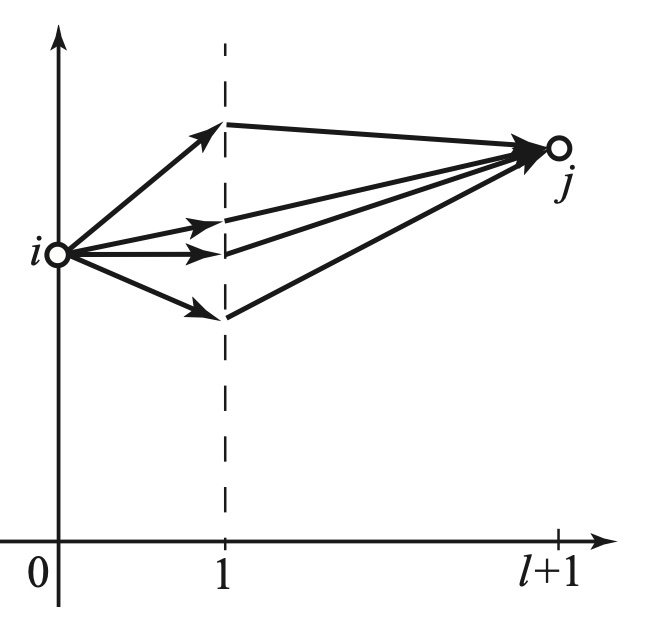
\includegraphics[width=0.5\linewidth]{Ger0r0r_pic_n_1.jpg} \\ а)}
    \end{minipage}
    \hfill
    \begin{minipage}[h]{0.49\linewidth}
    \center{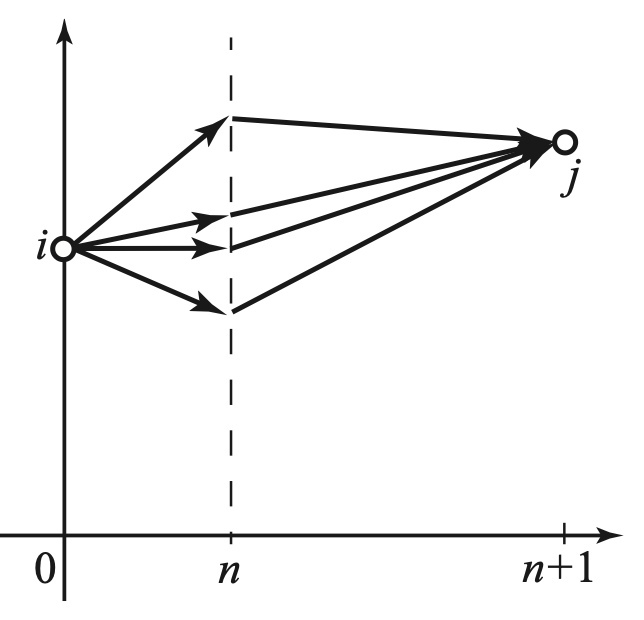
\includegraphics[width=0.5\linewidth]{Ger0r0r_pic_l_1.jpg} \\ б)}
    \end{minipage}
    \caption{а) Обратное уравнение б) Прямое уравнение}
\end{figure}

Из обратного уравнения следует
$$P^{(l)} = PP^{(l - 1)} = ... = P^l$$

где $P^{(l)} = \left| p_{ij}^{(l)}\right|$  - матрица вероятностей переходов за $l$ шагов; Р - матрица вероятностей переходов за 1 шаг. Т.е. для того, чтобы получить матрицу вероятностей переходов за $l$ шагов необходимо матрицу перехода за 1 шаг возвести в степень $l$.

\subsection{Нахождение вероятностей переходов с помощью производящих функций} 

Рассмотрим однородную цепь Маркова с дискретным временем и конечным числом состояний $X = \{1, 2, ..., N\}$. Прямое уравнение Чепмена-Колмогорова \eqref{eq-4} для нее можно переписать в виде

\begin{equation}\label{eq-5}
	p_{ij}^{(n)} = sum_{k = 1}^{N} p_{ik}^{(n - 1)}p_{kj}, i,j = \overline{1, N}, n \geq 2
\end{equation}

Данное соотношение обычно используют для вычисления $p_{ij}^{(n)}$ при небольших $n$. При больших $n$ используют следующий метод.
\par\medskip

Обозначим

\begin{equation}\label{eq-6}
    p_{ij}^{(0)} = \delta_{ij} = 
    \begin{cases}
      1, i = j
      \\
      0, i \neq j
    \end{cases}
\end{equation}

Тогда уравнение \eqref{eq-5} выполняется $при n = 1$, что можно проверить прямой подстановкой. Введем в рассмотрение производящие функции:
$$\psi_{ij}(z) = \sum_{n = 0}^{\infty} p_{ij}^{(n)}z^{n} $$

Ряд в правой части сходится по меньшей мере при $|z| < 1$, так как $0 \leq p_{ij}^{(n)} \leq 1$. Умножив обе части равнения \eqref{eq-5} на $z^{n}$ и просуммировав по $n$ от 1 до $\infty$, получим
$$\sum_{n = 1}^{\infty}p_{ij}^{(n)}z^n = \sum_{n = 1}^{\infty} \sum_{k = 1}^{N} p_{ik}^{(n - 1)}z^n p_{kj}$$

или
$$\sum_{n = 0}^{\infty}p_{ij}^{(n)}z^n -  p_{ij}^{(0)} = z \sum_{n = 0}^{\infty} \sum_{k = 1}^{N} p_{ik}^{(n)}z^n p_{kj}$$

Отсюда следует, что
$$\psi_{ij}(z) - p_{ij}^{(0)} = z \sum_{k = 1}^{N} \psi_{ik}(z) p_{kj}$$

Подставив в это равенство \eqref{eq-6}, получим

\begin{equation}\label{eq-7}
	\psi_{ij}(z) - z \sum_{k = 1}^{N} \psi_{ik}(z) p_{kj} = \delta_{ij}, i,j = \overline{1, N}
\end{equation}

Получили систему $N^2$ уравнений с $N^2$ неизвестными. Однако, так как в левую и правую часть равенства \eqref{eq-7} входит одно и то же $i$, можно отдельно решить $N$ уравнений при фиксированном $i$.
\par\medskip

Обозначим через $\Delta(z)$ определитель данной системы (один и тот же для всех $i$).

\begin{equation}\label{eq-8}
	\Delta(z) = \left|
	\begin{array}{cccc}
	1 - zp_{11} & -zp_{21} & \ldots & -zp_{N1}\\
	-zp_{12} & 1 - zp_{22} & \ldots & -zp_{N2}\\
	\vdots & \vdots & \ddots & \vdots\\
	-zp_{1N} & -zp_{2N} & \ldots & 1 - zp_{NN}
	\end{array}
	\right|
\end{equation}

При малом $|z|$ диагональные элементы близки к 1, а недиагональные - к 0, т.е. опеределитель $\Delta(z)$ близок к 1. Значит, $\Delta(z) \neq 0$ в некоторой окрестности точки $z = 0$  система уравнений \eqref{eq-7} имеет единственное решение.
\par\medskip

Так как коэффициенты этих уравнений - линейные функции, то 

\begin{equation}\label{eq-9}
	\psi_{ij}(z) = \frac{R_{ij}(z)}{S(z)}
\end{equation}

где $R_{ij}(z); S(z)$ - некоторые полиномы. Выражение \eqref{eq-9} после выделения целой части можно разложить на простейшие дроби вида $\frac{\beta_r}{(1 - \alpha_r z)^{r + 1}}$, где $\beta_r; \alpha_r$ - некоторые комплексные постоянные, $r = 0,1,2,...$.

\par\medskip

Далее будем исходить из тождества

\begin{equation}\label{eq-10}
	sum_{n = 0}^{\infty}\alpha^{n}z^{n} = \frac{1}{1 - \alpha z}
\end{equation}

Продифференцировав его $r$ раз, получим
$$\sum_{n = r}^{\infty} n(n - 1)\cdot...\cdot(n - r + 1)\alpha^{n} z^{n - r} = \frac{\alpha^{r}r!}{(1 - \alpha z)^{r + 1}} $$

или, что то же самое
$$\frac{1}{r!} \sum_{n = r}^{\infty} (n + r)(n + r - 1)\cdot...\cdot(n + 1)\alpha^{n} z^{n} = \frac{1}{(1 - \alpha z)^{r + 1}} $$

Таким образом, каждой элементарной дроби вида $\frac{\beta}{(1 - \alpha z)^{r + 1}}$, $r = 1,2,...$, соответствует составляющая $p_{ij}^{(n)}$ вида $\frac{\beta}{r!} (n + r)\cdot(n + r - 1) \cdot ... \cdot (n + 1)\alpha^{n}$; дроби вида $\frac{\beta}{1 - \alpha z}$ соответствует составляющая $p_{ij}^{(n)}$ вида $\beta \alpha^{n}$. Следовательно, $p_{ij}^{(n)}$ равно конечной сумме всех этих составляющих. 

\par\medskip
Описанным способом можно найти пределы $\lim_{n \rightarrow \infty} p_{ij}^{(n)}$, если они существуют.


\newpage
% Критерий существования стационарного режима марковской цепи
\section{Критерий существования стационарного режима марковской цепи}

\textbf{Автор:} Миндиярова Рената, Б-01-009

\subsection{Определение марковской цепи}
     В схеме Бернулли с $\Omega = \{\omega: {\omega = (x_1, ... x_n), x_i=0,1}\}$   вероятность $p(\omega)$ каждого исхода $\omega$ задавалась формулой  
\begin{equation} \label{mindiiarova_eq_1} 
p(\omega) = p(x_1)...p (x_n)
\end{equation}
 где $p(x)=p^xq^{1-x}$. При этом условии случайные величины $ \xi_1, ...,\xi_n$ с $\xi_n(\omega)=x_i$ оказывались независимыми и одинаково распределенными с 
\begin{center}
$P(\xi_1 = x) = ... = P(\xi_n = x) = p(x), x = 0,1 $
\end{center}

Если вместо (\ref{mindiiarova_eq_1}) положить 
\begin{center}
$p(\omega) = p_1 (x_1)...p_n (x_n)$,
\end{center}

 где $p_i(x)=p^x_i(1-p_i)^{1-x}$, $0\leq	p_i\leq	1$, то тогда случайные величины $ \xi_1, ...,\xi_n$ также будут \textit{независимыми}, но уже, вообще говоря, \textit{разнораспределенными}:
\begin{center}
$P(\xi_1 = x) = p_1 (x), ..., P(\xi_n = x) = p_n (x)$
\end{center}

Рассмотрим теперь одно обобщение этих систем, приводящее к \textit{зависимым} случайным величинам, образующим так называемую цепь Маркова.


Будем предполагать, что
\begin{center}
$\Omega = \{ \omega: \omega = (x_0, x_1, ..., x_n), x_i \in X \} $,
\end{center}
где X - некоторое конечное множество. Пусть заданы также неотрицательные функции $p_0(x), p_1(x,y), ..., p_n(x,y)$ такие, что 

\begin{equation} \label{mindiiarova_eq_2} 
\sum\limits_{x \in X} p_0 (x) = 1,\sum\limits_{y \in X} p_k (x, y) = 1, k = 1, ..., n; y \in X
\end{equation}

Для каждого исхода $\omega = (x_0, x_1, ..., x_n)$ положим
\begin{equation} \label{mindiiarova_eq_3} 
p(\omega) = p_0 (x_0) p_1 (x_0, x_1)...p_n (x_{n-1}, x_n)
\end{equation}

Нетрудно проверить, что $\sum\limits_{\omega \in \Omega} p(\omega) = 1$ и,
следовательно, набор этих чисел p($\omega)$ вместе с пространством $\Omega$ и системой всех его подмножеств опредяляет некоторую вероятностную модель, которую принято называть \textit{моделью испытаний, связанных в цепь Маркова}.


Введем в рассмотрение случайные величины $\xi_0, \xi_1, ...,\xi_n$ с 
    $\xi_i(\omega)=x_i$. Простой подсчет показывает, что
\begin{equation} \label{mindiiarova_eq_4} 
P(\xi_0 = a) = p_0(a), P(\xi_0 = a_0, ..., \xi_k = a_k ) = p_0(a) p_1(a_0, a_1)...p_1(a_{k-1}, a_k)
\end{equation}
Из (4) следует простое свойство условных вероятностей:
\begin{equation} \label{mindiiarova_eq_5} 
P \{ \xi_{k+1} = a_{k+1} | \xi_{k} = a_{k}, ..., \xi_{0} = a_{0} \} = P \{ \xi_{k+1} = a_{k+1} | \xi_{k} = a_{k}\}
\end{equation}

\begin{center}
(в предположении  $ P (\xi_k = a_k, ..., \xi_0 = a_0) > 0)$
\end{center}

Пусть $\mathscr{D}^\xi_k = \mathscr{D}_{\xi_0, ..., \xi_k} $ --разбиение, порожденное величинами  $ \xi_0, \xi_1, ...,\xi_k$, и $\mathscr{B}^\xi_k=\alpha(\mathscr{D}^\xi_k) $.


Из (\ref{mindiiarova_eq_5}) следует, что

\begin{equation} \label{mindiiarova_eq_6} 
P \{ \xi_{k+1} = a_{k+1} | \mathscr{B}^{\xi}_k \} = P \{ \xi_{k+1} = a_{k+1} | \xi_k\}
\end{equation}
или
\begin{equation} \label{mindiiarova_eq_7} 
P \{ \xi_{k+1} = a_{k+1} |\xi_0, ...,\xi_k \} = P \{ \xi_{k+1} = a_{k+1} | \xi_k\}
\end{equation}

Если воспользоваться очевидным равенством
\begin{equation} \label{mindiiarova_eq_8} 
P \text(AB|C) = P \text(A|BC) P \text(B|C)
\end{equation}

то из (\ref{mindiiarova_eq_6}) получаем, что
\begin{equation} \label{mindiiarova_eq_9} 
P \{ \xi_n = a_n, ..., \xi_{k+1} = a_{k+1} | \mathscr{B}^{\xi}_k \} = P \{ \xi_n = a_n, ..., \xi_{k+1} = a_{k+1} | \xi_k\}
\end{equation}
или  
\begin{equation} \label{mindiiarova_eq_10} 
P \{ \xi_n = a_n, ..., \xi_{k+1} = a_{k+1} |\xi_0, ...,\xi_k  \} = P \{ \xi_n = a_n, ..., \xi_{k+1} = a_{k+1} | \xi_k\}
\end{equation}

Это равенство допускает следующую наглядную интерпретацию. Будем трактовать
$\xi_k$ как положение частицы в "настоящем",  $(\xi_0, ...,\xi_{k-1})$ - в "прошлом" и   $(\xi_{k+1}, ...,\xi_n)$ - в "будущем". Тогда (\ref{mindiiarova_eq_10}) означает, что при фиксированных "прошлом" $(\xi_0, ...,\xi_{k-1})$ и "настоящем"  $\xi_k$ и не зависит от того, каким способом частица попала в точку $\xi_k$, т.е не зависит от "прошлого" $(\xi_0, ...,\xi_{k-1})$.


Пусть $\text{Б}$ = $\{\xi_n = a_n, ..., \xi_{k+1} = a_{k+1}\} $, $H = \{\xi_k=a_k\}$, $ \text{П} =  \{\xi_{k-1} = a_{k-1}, ..., \xi_0 = a_0\}$.
Тогда из (\ref{mindiiarova_eq_10}) следует, что
\begin{center}
$P($Б$|$НП$) = P($Б$|$Н$)$
\end{center} 
откуда следует, что
\begin{equation} \label{mindiiarova_eq_11} 
P(\text{БП|Н}) = P(\text{Б|Н})P(\text{П|Н})
\end{equation}
Иначе говоря, из (\ref{mindiiarova_eq_6}) следует, что при фиксированном "настоящем" Н, "будущее" Б и "прошлое" П оказываются независимыми. Нетрудно показать, что справедливо и обратное: из выполнения (\ref{mindiiarova_eq_11}) для любого $k = 0, 1, ..., n-1$
следует выполнение свойства (\ref{mindiiarova_eq_6}) для всякого $k = 0, 1, ..., n-1$.


Свойство независимости "будущего" и "прошлого", или, что то же, независимость "будущего" от "прошлого" при фиксированном "настоящем" принято называть \textit{марковским свойством}, а соответсвующую последовательность случайных величин   $(\xi_{0}, ...,\xi_n)$ - \textit{марковской цепью}.


Таким образом, если вероятности $p(\omega)$ элементарных событий задаются формулой (\ref{mindiiarova_eq_3}) то последовательность  $\xi = (\xi_0, ...,\xi_n)$ c $\xi_i(\omega)=x_i$, будет образовывать марковскую цепь.


В этой связи понятно следующее:


\begin{definition}
Пусть $(\Omega,  \mathscr{A}, P)$ - некоторое (конечное) вероятностное пространство и $\xi = (\xi_0, ...,\xi_n)$ - последовательность случайных величин со значениями в (конечном) множестве X. Если выполнено условие (\ref{mindiiarova_eq_6}), то последовательность $\xi = (\xi_0, ...,\xi_n)$ называется (конечной) \textit{марковской цепью}.


Множество X называется \textit{фазовым пространством}или \textit{пространством состояний} цепи. Набор вероятностей $(p_n(x)))$, $x\in X$, c $(p_0(x))) = P(\xi_0=x)$ называют \textit{начальным распределением}, а матрицу 
$
\begin{Vmatrix}
    p_k (x,y)
\end{Vmatrix}
$
, $x,y \in X$, c  $(p_k(x, y))) = P(\xi_k=y|\xi_{k-1}=x)$ - \textit{матрицей переходных вероятностей} (из состояний x в состояние y) в момент $k = 1, ..., n$.


В том случае, когда переходные вероятности $p_k(x, y))$ не зависят от 
$k,p_k(x, y)) = p(x, y))$, последовательность $\xi = (\xi_0, ...,\xi_n)$ называется однородной марковской цепью с матрицей переходных вероятностей 
$\begin{Vmatrix}
    p(x,y)
\end{Vmatrix}$
\end{definition}

Заметим, что матрица 
$\begin{Vmatrix}
    p(x,y)
\end{Vmatrix}$
является \textit{стохастической}: ее элементы неотрицательны и сумма элементов любой ее строки равна единице,  $\sum\limits_{y}p(x, y) = 1 , x \in X$.

Будем считать, что фазовое пространство X состоит из конечного множества целочисленных точек $(X = \{0, 1,... , N\}, X = \{0, \pm1, ..., \pm{N}\}$и т.д.) и обозначать $p_i=p_0(i)$ и $p_{ij} = p(i, j)$. а 


Понятно, что свойства однородных марковских цепей полностью определяются начальными распределниями $p_i$ и переходными вероятностями $p_{i j}$. В конкретных случаях для описания эволюции цепи вместо явного выписывания матрицы $\begin{Vmatrix}
    p(x_i,y_j)
\end{Vmatrix}$ используют (ориентированный) граф, вершинами которого являются состояния их X, а стрелка 

\begin{figure}[h]
\centering
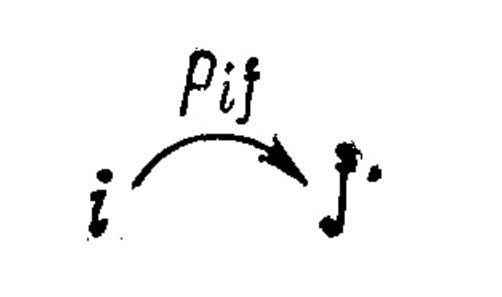
\includegraphics[width=0.2\linewidth]{mindiiarova_pic_1.jpg}
\label{fig:mpr}
\end{figure}


идущая из состояния i в состояние j и с числом $p_{ij}$ над ней, показывает, что из точки i возможен переход в точку j с вероятностью $p_{ij}$. В том случае, когда $p_{ij} = 0$, соответствующая стрелка не проводится.

\subsection{Эргодическая теорема}

Следующая теорема описывает широкий класс марковских цепей, обладающих так называем свойством \textit{эргодичности}: пределы  $\pi =  \lim_{n}p_{ij}^{(n)} $ не только существуют, не зависят от i, образуют распределение вероятностей ($\pi_j \geq 0, \sum\limits_{j}\pi_j = 1$, но и таковы, что $\pi_j > 0$ при всех j (такие распределения $\pi_j$ называются  \textit{эргодическими}).



\begin{theorem}

Пусть $\mathbb{P}$ =  
$\begin{Vmatrix}
    p_{ij}
\end{Vmatrix}  $
- \textit{матрица переходных вероятностей марковской цепи с конечным множеством состояний $X = \{1, 2, ..., N\}$}.

\begin{enumerate}[label=\alph*)]
\item  Если \textit{найдется $n_0$ такое, что} 
\begin{equation} \label{mindiiarova_eq_12} 
    \min_{i,j}p_{ij}^{(n_0)}>0,
\end{equation}
то существуют числа $\pi_1, ..., \pi_N$ такие, что
\begin{equation} \label{mindiiarova_eq_13} 
    \pi_j > 0,  \sum\limits_{j}\pi_j = 1
\end{equation}
и для любого $i \in X$
\begin{equation} \label{mindiiarova_eq_14} 
    p_{ij}^{(n)} \rightarrow \pi_j ,  n \rightarrow \infty.
\end{equation}

\item Обратно, если сущесвуют числа $\pi_1, ..., \pi_N$, удовлетворяющие условиям (\ref{mindiiarova_eq_13}) и (\ref{mindiiarova_eq_14}), то найдется $n_0$ такое, что выполненое условие (\ref{mindiiarova_eq_12}).

\item Числа  $(\pi_1, ..., \pi_N)$ удовлетворяют системе уравнений
\begin{equation} \label{mindiiarova_eq_15} 
    \pi_j = \sum\limits_{\alpha}\pi_{\alpha}p_{\alpha j}, j = 1, ..., N
\end{equation}
\end{enumerate}

\end{theorem}


\begin{proof}

a) Обозначим
\begin{equation} \label{mindiiarova_eq_16} 
      m_j^{(n)} = \min_{i}p_{ij}^{(n)}, M_j^{(n)} = \max_{i}p_{ij}^{(n)}
\end{equation}
Поскольку
\begin{equation} \label{mindiiarova_eq_17} 
      p_{ij}^{(n+1)} =  \sum\limits_{\alpha}p_{\alpha j}p_{\alpha j}^{(n)}
\end{equation}
то
\begin{equation}\label{mindiiarova_eq_18} 
      m_{j}^{(n+1)} =  \min_{i}p_{ij}^{(n+1)} =  \min_{i}\sum\limits_{\alpha}p_{i \alpha}p_{\alpha j}^{(n)} \geq \min_{i}\sum\limits_{\alpha}p_{i \alpha}\min_{\alpha}p_{\alpha j}^{(n)} = m_j^{(n)},
\end{equation}
откуда $m_j^{(n)} \leq m_j^{(n+1)}$ и аналогично $M_j^{(n)} \geq M_j^{(n+1)}$. Поэтому для доказательства утверждения (14) достаточно показать, что 
\begin{equation} \label{mindiiarova_eq_19} 
     M_j^{(n)} - m_j^{(n)} \rightarrow 0, 
     n \rightarrow \infty, j =1, ..., N.
\end{equation}
Пусть $\varepsilon = \min_{i, j}p_{ij}^{(n_0)} > 0$. Тогда

\begin{multline} \label{mindiiarova_eq_20} 
     p_{i j}^{(n_0+n)} = \sum\limits_{\alpha}p_{i \alpha}^{(n_0)}p_{\alpha j}^{(n)} =\sum\limits_{\alpha}(p_{i \alpha}^{(n_0)} - \varepsilon p_{\alpha j}^{(n))})p_{\alpha j}^{(n)} +\varepsilon\sum\limits_{\alpha}p_{j \alpha}^{(n)}p_{\alpha j}^{(n)} = \
     \\
   = \sum\limits_{\alpha}(p_{i \alpha}^{(n_0)} - \varepsilon p_{\alpha j}^{(n))})p_{\alpha j}^{(n)} + \varepsilon p^{(2n)}_{j j}.
\end{multline}
Но $p_{i \alpha}^{(n_0)} - \varepsilon p_{\alpha j}^{(n))} \geq 0$, поэтому 
\begin{equation} \label{mindiiarova_eq_21} 
     p_{ij}^{(n+n_0)} \geq m_j^{(n)} \cdot \sum\limits_{\alpha}(p_{i \alpha}^{(n_0)} - \varepsilon p_{\alpha j}^{(n))}) + \varepsilon p^{(2n)}_{i j} = m_j^{(n)}(1-\varepsilon)+\varepsilon p^{(2n)}_{j j},
\end{equation}
и, значит, 
\begin{equation} \label{mindiiarova_eq_22} 
     m_j^{(n_0+n)} \geq m_j^{(n)}(1-\varepsilon)+\varepsilon p^{(2n)}_{i j}
\end{equation}
Аналогичным образом
\begin{equation} \label{mindiiarova_eq_23} 
     M_j^{(n_0+n)} \leq M_j^{(n)}(1-\varepsilon)+\varepsilon p^{(2n)}_{i j}
\end{equation}
Объединяя эти неравенства, получаем
\begin{equation} \label{mindiiarova_eq_24} 
     M_j^{(n_0+n)} - m_j^{(n_0+n)} \leq (M_j^{(n)} - m_j^{(n)}) \cdot(1-\varepsilon)
\end{equation}
и, следовательно,
\begin{equation}\label{mindiiarova_eq_25} 
     M_j^{(kn_0+n)} - m_j^{(kn_0+n)} \leq (M_j^{(n)} - m_j^{(n)}) \cdot(1-\varepsilon)^k \rightarrow  0, k  \rightarrow \infty.
\end{equation}
Итак, по некоторой подпоследовательности \{$n_\beta$\} $M_j^{(n_\beta)} - m_j^{(n_\beta)}  \rightarrow 0, n_\beta \rightarrow \infty$. Но разность $M_j^{(n)} - m_j^{(n)}$ монотонна по n, а значит, $M_j^{(n)} - m_j^{(n)}  \rightarrow 0, n_\beta \rightarrow \infty$.
Если обозначить $\pi_j = \lim_{n} m_j^{(n)}$, то из полученных оценок следует, что для  $n \geq n_0$
\begin{equation} \label{mindiiarova_eq_26} 
     |p_{i j}^{(n)} - \pi_j| \leq M_j^{(n)} - m_j^{(n)} \leq (1-\varepsilon)^{(n/n_0) - 1},
\end{equation}
т.е сходимость $p_{i j}^{(n)}$ к предельным значеним $\pi_j$ происходит с геометрической скорость.

Ясно также, что $m_j^{(n)} \geq  m_j^{(n_0)} \geq \varepsilon > 0, n \geq n_0$, и, значит, $\pi_j >0$.


b) Условие (\ref{mindiiarova_eq_12}) непосредственно следует из (\ref{mindiiarova_eq_14}), посколько число состояний конечно и $\pi_j >0$.


c) Уравнение (\ref{mindiiarova_eq_15}) вытекают из (\ref{mindiiarova_eq_14}) и (\ref{mindiiarova_eq_17}).

\end{proof}

\subsection{Стационарное распределение вероятностей}
 Система уравнений (\ref{mindiiarova_eq_15}) играет большую роль в теории марковских цепей.
 Всякое ее неотрицательное решение $(\pi_1, ..., \pi_N)$, удовлетворяющее условию $\sum\limits_{\alpha}\pi_{\alpha} = 1$, принято называть \textit{стационарным} или \textit{инвариантным}, распределением вероятностей для марковской цепи с матрицей вероятностей 
 $
 \begin{Vmatrix}
    p_{ij}
\end{Vmatrix}.$
Объяснение состоит в следующем.


Возьмем распределение $(\pi_1, ..., \pi_N)$ в качестве начального, $p_j=\pi_j$. Тогда 
\begin{equation} \label{trivial}
     p_j^{(n)} = \sum\limits_{\alpha}\pi_{\alpha}p_{\alpha j}= \pi_j
\end{equation}
и вообще $p_j^{(n)} =\pi_j$. Иначе говоря, если в качестве начального распределения взять  $(\pi_1, ..., \pi_N)$, то это распределение не будет изменяться со временем,т.е для любого k
\begin{equation} \label{trivial}
     P(\xi_k=j) =  P(\xi_0=j), j = 1, ..., N.
\end{equation}
Более того, с таким начальным распределением марковская цепь $\xi = (\xi, \Pi,\mathbb{P})$ будет \textit{стационарной}: совместное распределение вектора $(\xi_k, ..., \xi_{k+l})$ не зависит от k для любого l (предполагается, что $k+l\leq n$)


Условие (\ref{mindiiarova_eq_12}) гарантирует как существование пределов $\pi_j = \lim_{n}p_{i j }^{(n)}$, не зависящих от i, так и существование эргодического распределения, т.е распределение с $\pi_j>0$. Распределение $(\pi_1, ..., \pi_N)$ оказывается также и \textit{стационарным} распределением. Покажем сейчас, что набор $(\pi_1, ..., \pi_N)$ является \textit{единственным} стационарным распределением.


В самом деле, пусть $(\tilde{\pi_1}, ..., \tilde{\pi_N})$ -- еще одно стационарное распределение. Тогда
\begin{equation} \label{trivial}
     \tilde{\pi_j} = \sum\limits_{\alpha}\tilde{\pi}_{\alpha}p_{\alpha j} = 
     ... = \sum\limits_{\alpha}\tilde{\pi}_{\alpha}p_{\alpha j}^{(n)}
\end{equation}
и поскольку $p_{i j}^{(n)} \rightarrow  \pi_j$, то
\begin{equation} \label{trivial}
     \tilde{\pi}_j= \sum\limits_{\alpha}(\tilde{\pi}_{\alpha} \cdot p_{i j})=\pi_j.
\end{equation}
В связи с этими результатами возникают интересные и важные вопросы о достаточных, необходимых, а также необходимых и достаточных условиях, при которых: (A)  \textit{существуют} пределы $\pi_j=\lim_{n}p_{i j}^{(n)}$, не зависящие от i; (B) пределы $(\pi_1, ..., \pi_N)$ образуют  \textit{распределение вероятностей}; (C) пределы $(\pi_1, ..., \pi_N)$ образуют \textit{эргодическое} распределение вероятностей; (D) \textit{сущесвтвует} и при том \textit{единственное} стационарное распределение вероятностей.
\subsection{Дополнение}
\begin{definition}
Рассмотрим какой-нибудь (конечный) неупорядоченный набор $\tau = [t_1, ..., t_n]$ различных индексов $t_i in T, n \geq 1$ и пусть $\mathbb{P_{\tau}}$ — вероятностная мера на ($\mathbb{R^{\tau}}, \mathscr{B}(\mathbb{R^{\tau}}) $).  Будем говорить, что семейство вероятностных мер {$\mathbb{P_{\tau}}$}, где $\tau$ пробегает множество всех конечных неупорядоченныхнаборов, согласовано, если для любых наборов  $\tau = [t_1, ..., t_n]$ и $\sigma =[s_1, ..., s_k]$  таких, что $\sigma in \tau$ и для любого $B \in  \mathscr{B}(\mathbb{R^{\sigma}})$

 \begin{equation} \label{trivial}
\mathbb{P_{\sigma}}\{(x_{s_1}, ..., x_{s_k}):(x_{s_1}, ..., x_{s_k}) \in B\} = \mathbb{P_{\tau}}\{(x_{t_1}, ..., x_{t_k}):(x_{s_1}, ..., x_{s_k}) \in B\}
\end{equation}
\end{definition}


\begin{theorem}[Колмогорова о продолжении меры в ($\mathbb{R^{T}}, \mathscr{B}(\mathbb{R^{T}}) $)]
Пусть  $\mathbb{P_{\tau}}$ — семейство согласованных вероятностных мер на $\mathbb{R^{\tau}}, \mathscr{B}(\mathbb{R^{\tau}}) $.Тогда существует, и притом единственная, вероятностная мера $\mathbb{P}$ на $\mathbb{R^{T}}, \mathscr{B}(\mathbb{R^{T}}) $, такая что $\mathbb{P}\{x \in \mathbb{R^{T}} : (x_{t_1}, ..., x_{t_k}) \in B\}  = \mathbb{P}_{[t_1, ..., t_n](B)}$ для
всех неупорядоченных наборов $\tau = [t_1, ..., t_n]$ различных индексов $t_i \in T$ и $B \in  \mathscr{B}$ (другими словами,$ \mathbb{P_{\tau}} = (\pi_{(T\rightarrow \tau)})_{*}\mathbb{P}$)
\end{theorem}

\begin{proof}
1. Отметим прежде всего, что если T не более чем счётно, то по предыдущей
теорема такая мера существует и единственна. Действительно, зафиксировав нумерацию $T = \{t_1, t_2, ...\}$ и воспользовавшись изоморфизмом $\mathbb{R^{T}} \cong \mathbb{R^{{\infty}}}$, по теореме  можем построить меру на $\mathbb{R^{T}}$, используя $\mathbb{P}_{n} = \mathbb{P}_{\{t_1,...,t_n\}}$. Построенная мера $\mathbb{P}$ будет удовлетворять равенству $ \mathbb{P_{\tau}} = (\pi_{(T\rightarrow \tau)})_{*}\mathbb{P}$ для
$\tau = \{t_1, ..., t_n\}, n \geq 1 $, и будет единственной с этим свойством. Чтобы доказать это свойство для произвольного конечного $\tau$, выберем $n$ так, что $\tau \in \{t_1, ..., t_n\} = \tau' $. Тогда
\begin{equation}
    \mathbb{P_{\tau}} = (\pi_{\tau' \rightarrow \tau})_{*} \mathbb{P}_{n} =  (\pi_{\tau' \rightarrow \tau})_{*}(\pi_{T \rightarrow \tau'})_{*}  \mathbb{P} = (\pi_{\tau' \rightarrow \tau})(\pi_{T \rightarrow \tau'})_{*}  \mathbb{P} = (\pi_{T \rightarrow \tau})_{*}  \mathbb{P}
\end{equation}
2. Пусть теперь T произвольно. Рассмотрим $M  \in  \mathscr{B}(\mathbb{R^{T}})$ По предложению $M \in \mathscr{B}_s$, т.е. $M = \pi^{-1}_{(T \rightarrow S)}(M_s)$ для некоторого не более чем счётного S и $M  \in  \mathscr{B}(\mathbb{R^{S}})$.. Применив теорему к множеству S и мерам $\mathbb{P}_{\tau}, \tau \in S$, получим меру $ \mathbb{P}_{s}$. Теперь положим
\begin{equation}
     \mathbb{P}(M) :=   \mathbb{P}_{s}(M_{s}) 
\end{equation}
Покажем, что так определённая мера $ \mathbb{P}$ будет корректно определена и $\sigma$ аддитивна. (Требуемая в теореме единственность будет вытекать из единственности мер $ \mathbb{P}_{s}$.)
Если $M \in \mathscr{B}_{s_1} $ и $M \in \mathscr{B}_{s_2} $, то $M \in \mathscr{B}_{s_1 \cup s_2}$, поэтому при проверке корректности можно
ограничиться случаем $S \in S'$. Итак, $M = \pi^{-1}_{(T \rightarrow S)}(M_s) = \pi^{-1}_{(T \rightarrow S')}(M'_s).$ Но тогда
\begin{equation}
   \pi^{-1}_{(T \rightarrow S')}(M'_s) =  \pi^{-1}_{(T \rightarrow S)}(M_s) =  \pi^{-1}_{(T \rightarrow S')} \pi^{-1}_{(S' \rightarrow S)} (M_s) 
\end{equation}
Поскольку $\pi_{(T \rightarrow S')}$ сюръективно, отсюда следует, что $M'_{S} = \pi^{-1}_{(S' \rightarrow S)} (M_s) $. . Но тогда корректность
сводится к равенству 
\begin{equation}
    \mathbb{P}_{S'}(\pi^{-1}_{(S' \rightarrow S)} (Y)) =  \mathbb{P}_{S}(Y)
\end{equation}
для $Y = M_s$. Его истинность при всех $Y \in \mathscr{B}(\mathbb{R^{S}}) $
следует из того факта, что обе части 35 как функции от Y удовлетворяют условиям теоремы для множества $S$ и мер $ \mathbb{P}_{\tau}, \tau \in S$, а значит, совпадают.
\end{proof}
 


\begin{remark} Исходное семейство вероятностных мер \{$\mathbb{P}_{\tau}$\} предполагалось заданным для всех неупорядоченных наборов $\tau = [t_1,...,t_n] $ различных индексов. Однако можно было начать и с семейства вероятностных мер $\mathbb{P}_{\tau}$, где $\tau$ пробегает семейство всех {\it упорядоченных} наборов  $\tau = (t_1,...,t_n)$ различных индексов. В таком случае для справедливости только что доказанной теоремы Колмагорова необходимо добавить дополнительное условие согласованности, а именно
\begin{equation}
\mathbb{P}_{(t_1, ...t_n)}(A_{t_1}\times...\times A_{t_n}) = \mathbb{P}_{(t_{i_1}, ...t_{i_n})}(A_{t_{i_1}}\times...\times A_{t_{i_n}})
\end{equation}
где $(i_1, ..., i_n)$ есть перестановка чисел $(1,...,n)$, а $A_{t_i} \in \mathfrak{B}(\mathbb{R}_{t_i})$. Нетрудно видеть, что это условие является необходимым для существования меры $\mathbb{P}$, о которой говорится в условии теоремы Колмогорова . Детали мы оставляем читателю, отметим лишь, что 36 есть частный случай равенства $\mathbb{P}_{(t_1, ...t_n)} = (f_{\sigma})_*{P}_{(t_{\sigma(1)}, ...t_{\sigma(n)})}$, где $f_{\sigma}$ переставляет координаты в $\mathbb{R}^n$ согласно перестановке $\sigma$.
\end{remark}








\newpage
%  Среднее время возвращения марковской цепи в существенное состояние
\section{Среднее время возвращения марковской цепи в существенное состояние}

\textbf{Автор:} Софья Бочкарёва, Б-01-005

\subsection{Основные понятия} 
\textbf{Марковским процессом} называется случайный процесс $\xi (t)$, если его условная плотность распределения не зависит от значений процесса в моменты $t_1, t_2, ..., t_{n-1}$ а определяется лишь значением $\xi(t_n) = x_n$, т.е.

$$p(x_{n + 1}, t_{n + 1} | x_1, t_1; x_2, t_2;...;x_n, t_n) = p(x_{n + 1}, t_{n + 1} | x_n, t_n)$$

\textbf{Марковской цепью} называют марковский процесс, для которого множество $X = \{i_1, i_2, ..., i_n, ...\}$ счетно или конечно. 
\par\medskip
Рассмотрим цепь Маркова с дискретным временем и, для простоты, с конечным числом состояний $X = \{1, 2, ... N\}$. Вероятности

$$p_{ij}^{(n)} = P(\xi_{m+n} = j | \xi_m = i), n \geq 1, m \geq 1, i,j \in X $$

называются \textit{вероятностями перехода цепи Маркова за n шагов}, а $p_{ij}^{(1)} = p_{ij}$ просто \textit{вероятностями перехода}. Матрица вида

\begin{equation*}
	P = \left(
	\begin{array}{cccc}
	p_{11} & p_{12} & \ldots & p_{1N}\\
	p_{21} & p_{22} & \ldots & p_{2N}\\
	\vdots & \vdots & \ddots & \vdots\\
	p_{N1} & p_{N2} & \ldots & p_{NN}
	\end{array}
	\right)
\end{equation*}

называется \textit{матрицей вероятностей перехода цепи Маркова}.
\par\medskip
\textbf{Однородной} называется цепь Маркова, у которой вероятности перехода не зависят от m, т.е. матрица $P$ не зависит от шага m. Тогда очевидно, что свойства однородной марковской цепи зависят только от матрицы $P$ и начального распределения
\par\medskip
\textbf{Несущественным состоянием $i \in X$} называется состояние, из которого можно за положительное число шагов выйти: $\exists m, j : p_{ij}^{(m)} > 0$, но нельзя в него вернуться: \mbox{$\forall n : p_{ij}^{(n)} = 0$.}
\par\medskip
Если из множества $X$ всех состояний выделить несущественные, то оставшееся множество \textbf{существенных} состояний обладает тем свойством, что, попав в него, цепь Маркова никогда из него не выйдет. 

\par\medskip
\textbf{Сообщающимися состояниями} i и j называются существенные состояния, если i достижимо из j, и j достижимо из i. Обозначается как $i \leftrightarrow j$.
\par\medskip
Множество существенных состояний разбивается на конечное или счетное число непересекающихся множеств $X_1, X_2, ...$ состоящих из сообщающихся состояний и характеризующихся тем, что переходы между различными множествами невозможны.
Тогда такие множества называют \textbf{классами} или \textbf{неразложимыми классами} существенных сообщающихся состояний. 

\par\medskip
Рассмотрим Марковскую цепь с дискретным временем. Введем в рассмотрение вероятности:

$$f_{ii}^(k) = P\{\xi_k = i; \xi_l \neq i, 1 \leq l \leq k - 1 | \xi_0 = i\}$$ - вероятность первого возвращения цепи Маркова из состояния i в состояние i на k-м шаге (в дискретный момент времени k). 

$$f_{ij}^(k) = P\{\xi_k = j; \xi_l \neq j, 1 \leq l \leq k - 1 | \xi_0 = i\}$$ - вероятность первого попадания цепи в состояние j к моменту времени k из исходного состояния i.

\par\medskip

\textbf{Эргодической цепью Маркова} называется такая цепь, для которой справедливо:

$$\lim_{n \to \infty} p_{ij}^{(n)}  = \pi_{j}, j \in X, \sum_{j \in X} \pi_j = 1$$

где $\{\pi_j \}$ -эргодическое распределение.

\subsection{О средних временах переходов между состояниями} 

Обозначим через $E$ множество состояний эргодического класса, $i,j \in E$. Через $m_{ij}$ обозначим среднее число шагов, необходимых для перехода из i-го состояния в j-е состояние. Найдем это число (что для цепи с дискретным временем равносильно времени перехода из состояния i в j).
За 1 шаг цепь может из состояния i с вероятностью $p_{ij}$ перейти в состояние j, тогда время перехода будет равняться 1. Соответственно, оно будет равняться $m_{ij} = 1 + m_{kj}$, если цепь перейдет в некоторое промежуточное состояние k.
Тогда по формуле для условного математического ожидания получаем:

$$ m_{ij} = 1 \cdot p_{ij} + \sum_{k \neq j} p_{ik}(m_{kj + 1})$$

или

$$ m_{ij} = 1 + \sum_{k} p_{ik}(m_{kj + 1}) - p_{ij}m_{jj} \qquad \qquad (1)$$


Введем матричные обозначения:

$$ M = \left| m_{ij} \right|, i,j, \in E$$

\begin{equation*}
	S = \left(
	\begin{array}{cccc}
	1 & 1 & \ldots & 1\\
	1 & 1 & \ldots & 1\\
	\vdots & \vdots & \ddots & \vdots\\
	1 & 1 & \ldots & 1
	\end{array}
	\right)
\end{equation*}

\begin{equation*}
	D = \left(
	\begin{array}{cccc}
	m_{11} & 0 & \ldots & 0\\
	0 & m_{22} & \ldots & 0\\
	\vdots & \vdots & \ddots & \vdots\\
	0 & 0 & \ldots & m_{rr}
	\end{array}
	\right)
\end{equation*}

где r - число состояний данного класса. Тогда систему уравнений (1) можно переписать в матричном виде:

$$M = S + PM - PD$$

\begin{center}
	$\Downarrow$
\end{center}

$$M = (I - P)^{-1} \cdot (SPD)$$

Данная формула определяет искомые средние значения времени перехода из одного состояния в другое.

\par\medskip

Рассмотрим теперь диагональные элементы матрицы $D$. Для этого умножим систему уравнений (1) на финальную вероятность i-го состояния $\pi_i$ и просуммируем по i:

$$\sum{i} \pi_i m_{ij} = 1 + \sum_{k}m_{kj}\sum_{i}\pi_i p_{ik} - m_{jj}\sum_{i} \pi_i p_{ij}$$

Тогда, с учетом эргодической теоремы для цепей Маркова ($\pi_j = \sum_{k = 1}^{N} \pi_k p_{kj}, j = \overline {\rm 1,N}$) приходим к равенству:

$$\sum{i} \pi_i m_{ij} = 1 + \sum_{k}\pi_k m_{kj} - \pi_j m_{jj}$$

откуда находим 

$$m_{jj} = \frac{1}{\pi_j}$$

Таким образом, \textit{среднее время возвращения цепи Маркова в существенное состояние обрано пропорционально финальной вероятности этого состояния}, что, в свою очередь, означает,
что среднее время возвращения в положительное возвратное состояние конечно, а в нулевое возвратное состояние - бесконечно. 


\newpage
% Классификация состояний марковской цепи на основе свойств неразложимости и апериодичности


\section{Классификация состояний марковской цепи на основе свойств неразложимости и апериодичности}

\textbf{Автор:} Мамыко Ксения Юрьевна, Б-01-001

\begin{definition}\label{oduvan_def_1} (марковская цепь в широком смысле)  Пусть $(\Omega, \mathscr{F}, {(\mathscr{F}_n)}_{n \geq 0}, \mathbf{P})~-$ фильтрованное вероятностное пространство и $(E, \mathscr{E})~-$ фазовое пространство. Последовательность $X = {(X_n)}_{n \geq 0}$ случайных элементов $X_n = X_n(\omega)$, заданных на $(\Omega, \mathscr{F}, {(\mathscr{F}_n)}_{n \geq 0}, \mathbf{P})$, принимающих значения в $E$ и являющихся
$\mathscr{F}_n/\mathscr{E}$ -измеримыми, $n \geq 0$, называется последовательностью величин, связанных \emph{марковской зависимостью (марковской цепью, цепью Маркова) в широком смысле}, если для любых $n \geq 0$ и $B \in \mathscr{E}$ выполнено \emph{марковское свойство в широком смысле}:

\begin{equation}\label{oduvan_eq_1}
    \mathbf{P}(X_{n+1} \in B| \mathscr{F}_n)(\omega) = \mathbf{P}(X_{n+1} \in B| X_n(\omega))
\end{equation}

\end{definition}

Если ${\mathscr{F}_n}^X = \sigma (X_0, X_1, \ldots, X_n)$ есть $\sigma$-алгебра, порожденная величинами $X_0, X_1, \ldots, X_n$, то, поскольку ${\mathscr{F}_n}^X \subseteq \mathscr{F}_n$, а $X_n~- {\mathscr{F}_n}^X$-измеримы, из (\ref{oduvan_eq_1}) получаем \emph{марковское свойство в узком смысле} (или просто \emph{марковское свойство}):

\begin{equation}\label{oduvan_eq_2}
    \mathbf{P}(X_{n+1} \in B| {\mathscr{F}_n}^X)(\omega) = \mathbf{P}(X_{n+1} \in B| X_n(\omega)) 
\end{equation}

Для наглядности это свойство записывают часто в
таком виде:

\begin{equation}\label{oduvan_eq_3}
    \mathbf{P}(X_{n+1} \in B|X_0(\omega), \ldots, X_n(\omega)) = \mathbf{P}(X_{n+1} \in B| X_n(\omega)) 
\end{equation}

Выведенное из (\ref{oduvan_eq_1}) марковское свойство в узком смысле (\ref{oduvan_eq_2}) подсказывает целесообразность введения понятия марковской зависимости и в том
случае, когда a priori не выделяется поток ${(\mathscr{F}_n)}_{n \geq 0}$.

\begin{definition}\label{oduvan_def_2}(марковская цепь) Пусть $((\Omega, \mathscr{F}, \mathbf{P}))$ вероятностное пространство, $(E, \mathscr{E})$ фазовое пространство. Последовательность $X = {(X_n)}_{n \geq 0}$ случайных элементов $X_n = X_n(\omega)$, принимающих значения
в $E$ и являющихся $\mathscr{F}/\mathscr{E}$-измеримыми, называется последовательностью величин, связанных \emph{марковской зависимостью (марковской цепью, цепью Маркова)}, если для любых $n \geq 0$ и $B \in \mathscr{E}$ выполнено \emph{марковское свойство в узком смысле} (\ref{oduvan_eq_2}).
\end{definition}

\begin{remark} Введение с самого начала фильтрованного вероятностного пространства, на котором определялась марковская цепь \emph{в широком смысле}, оказывается полезным во многих вопросах, где поведение
систем рассматривается в зависимости от того или иного «потока информации» ${(\mathscr{F}_n)}_{n \geq 0}$. Например, может случиться, что у «двумерного» процесса $(X, Y) = (X_n, Y_n)_{n \geq 0}$ первая компонента $X = {(X_n)}_{n \geq 0}$, не будучи марковской в смысле определения (2), тем не менее является марковской в смысле определения (\ref{oduvan_def_1}) с ${\mathscr{F}_n} = {\mathscr{F}_n}^{X, Y}, n \geq 0$. В элементарном же изложении теории марковских цепей поток ${(\mathscr{F}_n)}_{n \geq 0}$ обычно не вводится и за
основу принимается определение \ref{oduvan_def_2}.
\end{remark}

Будем предполагать, что рассматриваемая марковская цепь имеет
\emph{счетное} множество состояний $E = \{1, 2, \ldots\}$ и переходные вероятности $p_{ij}, i,j \in E$. Матрицу (таблицу), образованную этими переходными вероятностями, будем обозначать $\mathbb {P} = \Vert p_{ij} \Vert$ или, в более развернутой форме,

\[ \mathbb {P} = \begin{Vmatrix}
  p_{11}& p_{12}& p_{13}& \cdots\\
  p_{21}& p_{22}& p_{23}& \cdots\\
  \cdots & \cdots & \cdots& \cdots\\
  p_{i1}& p_{i2}& p_{i3}& \cdots\\
  \cdots & \cdots & \cdots& \cdots
\end{Vmatrix}. \]

(Вместо $\Vert \cdot \Vert$ для матриц часто бывает удобнее писать ($\cdot$).)

Приводимая далее классификация состояний марковских цепей полностью определяется \emph{алгебраическими} свойствами матриц переходных вероятностей $\mathbb{P}$ и их степеней $\mathbb{P}^{(n)}$, $n \geq 1$.

Матрица переходных вероятностей $\mathbb{P}$ полностью определяет \emph{одношаговые} переходы из состояния в состояние. Матрицы же $\mathbb{P}^{(n)} = \Vert {p_{ij}}^{(n)} \Vert$ определяют (в силу марковского свойства) переходы за \emph{n шагов}.

Скажем, матрица

\[ \mathbb{P} = \begin{pmatrix}
  1/2& 1/2\\
  0& 1
\end{pmatrix}\]

и соответствующий ей граф показывают, что определяемое
ими \emph{движение} «частицы», блуждающей по состояниям 0 и 1, таково, что
за один шаг возможен переход 0 $\rightarrow$ 1 (с вероятностью 1/2), но переход 1 $\rightarrow$ 0 невозможен. Ясно, что переход 1 $\rightarrow$ 0 невозможен и за любое число шагов, что видно, конечно, и из структуры матриц

\[ \mathbb{P}^{(n)} = \begin{pmatrix}
  2^{-n} & 1 - 2^{-n}\\
  0& 1
\end{pmatrix}, \]

показывающей, что ${p_{10}}^{(n)} = 0$ при любом $n \geq 1$.

В этом примере состояние 1 является таким, что в него можно \emph{войти} (из состояния 0), но нельзя из него \emph{выйти}.

Рассмотрим граф на рис.~\ref{fig::oduvan_pic_1}, по которому легко восстановить и соответствующую матрицу переходов $\mathbb{P}$. Из вида этого графа ясно, что здесь
имеется три состояния (левая часть рисунка), выйдя из которых, обратно
вернуться невозможно.

С точки зрения «будущего» поведения «частицы», блуждающей в соответствии с данным графом, эти три состояния \emph{несущественны} (и называются \emph{несущественными}) по той указанной причине, что из них \emph{возможен
выход}, но в них \emph{невозможно возвращение}.

\begin{figure}[h!]
			\centering
			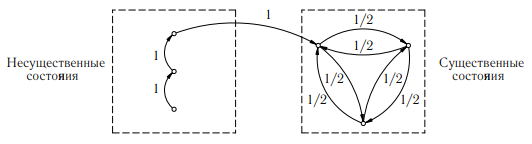
\includegraphics[width=0.6\linewidth]{oduvanchik_i_pic_1.png}
			\caption{~}
			\label{fig::oduvan_pic_1}
\end{figure}

Такие «несущественные» состояния, не представляющие интереса,
можно сразу отбросить, сосредоточив все внимание на классификации
лишь оставшихся «\emph{существенных}» состояний.

Чтобы расклассифицировать существенные состояния или группы
таких состояний, нам понадобится ряд определений.

\begin{definition} Говорят, что состояние $j$ \emph{достижимо} из состояния $i$ (обозначение: $i \rightarrow j$), если найдется такое $n \geq 0$, что ${p_{ij}}^{(n)} > 0$ (${p_{ij}}^{(0)} = 1$, если $i = j$, и 0, если $i \neq j$).

Состояния $i$ и $j$ называются \emph{сообщающимися} (обозначение: $i \leftrightarrow j$), если $i \rightarrow j$ и $j \rightarrow i$, т. е. они являются \emph{взаимно достижимыми}.
\end{definition}

\begin{lemma} Свойство сообщаемости «$\leftrightarrow$» (взаимной достижимости) есть отношение эквивалентности состояний (марковской цепи
с матрицей переходных вероятностей $\mathbb{P}$).
\end{lemma}

\begin{proof}По определению отношения эквивалентности (в данном случае отношения «$\leftrightarrow$») надо проверить его рефлексивность
($i\leftrightarrow i$), симметричность (если $i \leftrightarrow j$, то $j \leftrightarrow i$) и транзитивность (если
$i \leftrightarrow j$, $j \leftrightarrow k$, то $i \leftrightarrow k$).

Первые два свойства следуют непосредственно из определения сообщаемости состояний. Транзитивность вытекает из уравнения Колмогорова - Чепмена: если ${p_{ij}}^{(n)} > 0$, ${p_{jk}}^{(m)} > 0$, то

\[{p_{ik}}^{(n+m)} = \sum_{l \in E} {p_{il}}^{(n)} {p_{lk}}^{(m)} \geq {p_{ij}}^{(n)} {p_{jk}}^{(m)} > 0,\]

т. е. $i \rightarrow k$. Аналогично, $k \rightarrow i$. Тем самым, $i \leftrightarrow k$. \end{proof}

Будем относить все сообщающиеся между собой состояния $i, j, k, \ldots$
($i \leftrightarrow j$, $j \leftrightarrow k$, $k \leftrightarrow i$, $\ldots$) к одному \emph{классу}. Тогда любые такие классы состояний или совпадают, или же не пересекаются. Следовательно, отношение \emph{сообщаемости} разбивает все множество (существенных) состояний $E$ на конечное или счетное число непересекающихся множеств $E_1, E_2, \ldots (E = E_1 + E_2 + \ldots)$.

Эти множества будем называть \emph{неразложимыми классами} (существенных сообщающихся) состояний. Марковскую цепь, все состояния которой образуют \emph{один} неразложимый класс, будем называть \emph{неразложимой}.

Для иллюстрации введенных понятий рассмотрим цепь с пространством
состояний $E = \{ 1, 2, 3, 4, 5\}$ и матрицей переходных вероятностей

\[
\newcommand*{\temp}{\multicolumn{1}{r|}{}}
\mathbb{P} = \begin{pmatrix}
  1/3 & 2/3 &\temp & 0 & 0 & 0\\
  1/3 & 2/3 &\temp &0 & 0 & 0\\ \cline{1-6}
  0 & 0 &\temp &0 & 1 & 0\\
  0 & 0 &\temp &1/2 & 0 & 1/2\\
  0 & 0 &\temp &0 & 1 & 0
\end{pmatrix}
=
\begin{pmatrix}
  \mathbb{P}_1&\temp &0\\ \hline
  0&\temp &\mathbb{P}_2
\end{pmatrix}
.
\]

Граф этой цепи с \emph{пятью} состояниями имеет следующий вид:

\begin{figure}[h!]
    \centering
    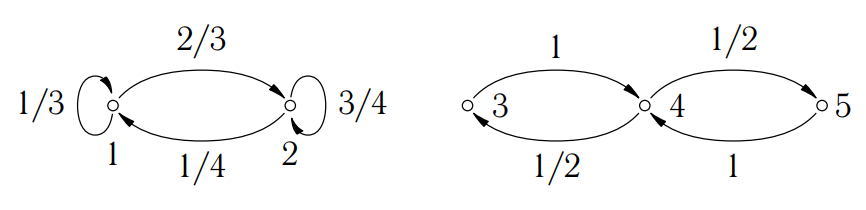
\includegraphics[width=0.5\linewidth]{oduvanchik_i_pic_2.png}
    \caption{~}
    \label{fig::oduvan_pic_2}
\end{figure}

\begin{wrapfigure}{r}{0.4\textwidth}
                \centering
			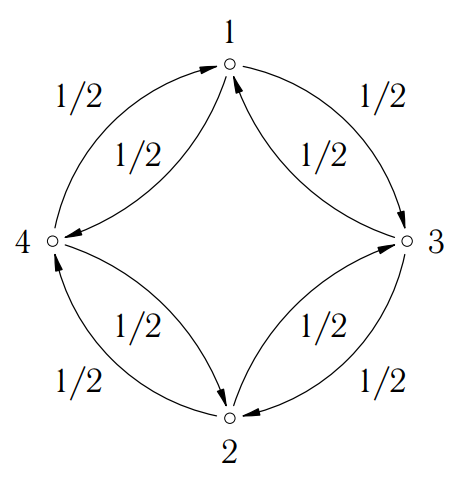
\includegraphics[width=0.6\linewidth]{oduvanchik_i_pic_3.png}
			\caption{Пример марковской цепи с периодом d = 2}
			\label{fig::oduvan_markov_chain_exm}
\end{wrapfigure}

Ясно, что у рассматриваемой цепи есть \emph{два} неразложимых класса $E_1 = \{1, 2\}$, $E_2 = \{3, 4, 5\}$, и исследование ее свойств сводится к исследованию свойств каждой из двух цепей, множествами состояний которых
являются множества $E_1$ и $E_2$, а матрицы переходных вероятностей равны соответственно $\mathbb{P}_1$ и $\mathbb{P}_2$.

Рассмотрим теперь какой-нибудь неразложимый класс $E$. Для примера пусть им будет класс, изображенный на рис.~\ref{fig::oduvan_pic_2}.



Заметим, что здесь возвращение в каждое состояние возможно лишь за \emph{четное} число шагов, переход в соседнее состояние$~-$ за \emph{нечетное} число шагов, а матрица переходных вероятностей имеет блочную структуру:

\[
\newcommand*{\temp}{\multicolumn{1}{r|}{}}
\mathbb{P} = 
\begin{pmatrix}
  0 & 0 & \temp &1/2 & 1/2\\
  0 & 0 & \temp &1/2 & 1/2\\ \cline{1-5}
  1/2 & 1/2& \temp & 0 & 0\\
  1/2 & 1/2&\temp & 0 & 0
\end{pmatrix}
.\]

Отсюда видно, что класс $E = \{1, 2, 3, 4\}$ разбивается на два подкласса
$C_0 =\{1, 2\}$ и $C_1 =\{3, 4\}$, обладающих следующим свойством \emph{цикличности}:
за один шаг из $C_0$ «частица» непременно переходит в $C_1$, а из $C_1$$~-$ в $C_0$.

Приведенный пример показывает, что, по-видимому, и в общем случае можно дать соответствующую классификацию \emph{неразложимых} классов состояний на \emph{циклические подклассы}.

С этой целью нам понадобятся некоторые определения и один факт из
теории чисел.

\begin{definition} Пусть $\varphi = (\varphi_1, \varphi_2, \ldots)~-$ некоторая последовательность неотрицательных чисел $\varphi_n \geq 0, n \geq 1$. \emph{Периодом} последовательности $\varphi$ (обозначение: $d(\varphi)$) называется число 

\[d(\varphi) = \text{НОД} \{n \geq 1 : \varphi_n > 0\},\]

где НОД$(M_{\varphi})$ есть \emph{Наибольший Общий Делитель} множества $M_{\varphi}$ тех индексов $n \geq 1$, для которых $\varphi_n > 0$; если $\varphi_n = 0, n \geq 1$, то 
$M_{\varphi} = \oslash$ и НОД($M_{\varphi}$) полагается равным нулю.
\end{definition}

По-другому можно сказать, что последовательность $\varphi$ имеет период
$d(\varphi)$, если из того, что $\varphi_n > 0$, следует, что $d(\varphi)$ делит $n$ (т. е. $n$ должно иметь вид $d(\varphi)k$ с некоторым $k \geq 1$) и $d(\varphi)$ является наибольшим среди всех тех чисел $d$, которые обладают таким свойством (т. е. таких, что $n=dl$ с некоторым целым $l \geq 1$).

Так, например, последовательность $\varphi = (\varphi_1, \varphi_2, \ldots)$ такая, что $\varphi_{4k} > 0$ для $k = 1, 2, \ldots$ и $\varphi_n = 0$ для $n \neq 4k$, имеет период $d(\varphi) =$ 4, а не 2, хотя $\varphi_{2l} > 0$ для $l = 2, 4, 8$.

\begin{definition} Говорят, что последовательность $\varphi = (\varphi_1, \varphi_2, \ldots)$ \emph{апериодическая}, если ее период $d(\varphi) = 1$.
\end{definition}

Следующий элементарный результат из теории чисел будет в дальнейшем полезен при классификации состояний по свойству цикличности.

\begin{lemma} Пусть $M~-$ некоторое множество неотрицательных
целых чисел ($M \subseteq E$), замкнутое относительно сложения и такое,
что НОД$(M) = 1$. Тогда при некотором $n_0$ все числа $n \geq n_0$ будут принадлежать $M$.
\end{lemma}

Применим эту лемму к множеству $M = M_{\varphi}$, беря в качестве последовательности $\varphi = (\varphi_1, \varphi_2, \ldots)$ последовательность $({p_{jj}}^{(1)}, {p_{jj}}^{(2)}, \ldots)$ или последовательность $({p_{jj}}^{(d)}, {p_{jj}}^{(2d)}, \ldots)$, $d \geq 1$, где $j~-$ некоторое состояние марковской цепи, имеющей матрицу переходных вероятностей $\mathbb{P} = \Vert p_{ij} \Vert$, а ${p_{jj}}^{(n)}~-$ элемент матрицы ${\mathbb{P}}^{(n)}, n \geq 1, {\mathbb{P}}^{(1)} = \mathbb{P}$. (При этом будем говорить, что
состояние $j$ имеет период $d(j)$, если $d(j)$ есть период последовательности
$({p_{jj}}^{(1)}, {p_{jj}}^{(2)}, \ldots)$.)  Тогда получим следующий результат.

\begin{theorem} \emph{Пусть состояние $j$ имеет период $d = d(j)$.}

\emph{Если $d = 1$, то найдется такое $n_0 = n_0 (j)$, что для всех $n \geq n_0$ переходные вероятности ${p_{jj}}^{(n)} > 0$.}

\emph{Если $d > 1$, то найдется такое $n_0 = n_0 (j, d)$, что для всех $n \geq n_0$ переходные вероятности ${p_{jj}}^{(nd)} > 0$.}

\emph{Если $d \geq 1$ и ${p_{ij}}^{(m)} > 0$ для некоторых $i \in E$ и $m \geq 1$, то найдется такое $n_0 = n_0(j, d, m)$, что ${p_{ij}}^{(m + nd)} > 0$  для всех $n \geq n_0$.}
\end{theorem}

Приведем теперь теорему, показывающую, что \emph{период} состояний неразложимого класса обладает свойством «однотипности».

\begin{theorem} \emph{Пусть ${E}_* =\{i, j, \ldots \}~-$ некоторый неразложимый класс (сообщающихся) состояний из множества $E$.}
\emph{Все состояния такого класса являются «однотипными» в том
смысле, что они имеют один и тот же период (обозначаемый $d(E_*)$
и называемый периодом класса $E_*$).}
\end{theorem}

\begin{proof}
Пусть $i, j \in E_*$. Тогда найдутся такие $k$ и $l$, что ${p_{ij}}^{(k)} > 0$ и ${p_{ji}}^{(l)} > 0$. Но тогда в силу уравнения Колмогорова$~–$ Чепмена
\[{p_{ii}}^{(k + l)} = \sum_{a \in E} {p_{ia}}^{(k)} {p_{ai}}^{(l)} \geq {p_{ij}}^{(k)} {p_{ji}}^{(l)} > 0,\]
и, значит, $k + l$ должно делиться на $d(i)~-$ период состояния $i \in E_*$.

Пусть $d(j)~-$ период состояния $j \in E_*$ и $n$ таково, что ${p_{jj}}^{(n)} > 0$. Тогда $n$ должно делиться на $d(j)$ и так как
\[{p_{ii}}^{(n + k + l)} \geq {p_{ij}}^{(k)} {p_{jj}}^{(n)} {p_{ji}}^{(l)} > 0,\]
то $n + k + l$ делится на $d(i)$. Но $k + l$ делится на $d(i)$, а значит, $n$ делится на $d(i)$ и поскольку $d(j) = \text{НОД}\{ n: {p_{jj}}^{(n)} > 0\}$, то $d(i) \leq d(j)$.

По симметрии $d(j) \leq d(i)$, и, следовательно, $d(i) = d(j)$.
\end{proof}

Если множество состояний $E_* \subseteq E$ образует неразложимый класс
(сообщающихся состояний) и $d(E_*) = 1$, то о таком классе говорят как об
\emph{апериодическом классе} состояний.

Рассмотрим теперь случай $d(E_*) \geq 1$.

Переходы из состояния в состояние внутри такого класса могут осуществляться весьма причудливым образом (как в рассмотренном выше примере марковской цепи с периодом $d(E_*) =2$; см. рис. \ref{fig::oduvan_pic_2}).

\begin{wrapfigure}{r}{0.4\textwidth}
                \centering
			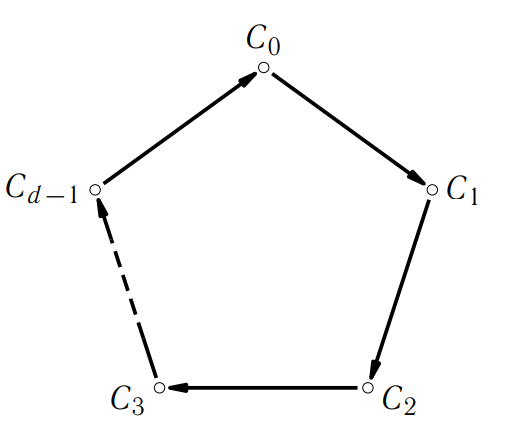
\includegraphics[width=0.6\linewidth]{oduvanchik_i_pic_4.png}
			\caption{Движение по циклическим подклассам}
			\label{fig::oduvan_cycle_motion}
\end{wrapfigure}
Оказывается, однако, что в этих переходах, из одной группы состояний в другую, имеет место вполне определенная «\emph{цикличность}»:


\begin{theorem} \emph{Пусть $E_*$ –– неразложимый класс состояний, $E_* \subseteq E$, с периодом $d = d(E_*) > 1$. Тогда найдутся $d$ групп состояний $C_0, C_1, \ldots , C_{d-1}$, называемых циклическими подклассами $(E_* = C_0 + C_1 + \ldots + C_{d-1})$, характеризуемые тем, что в моменты времени $n = p + kd$ с $p = 0, 1, \ldots , d - 1$ и
$k=0, 1, \ldots$ «частица» будет находиться в подклассе $C_p$ с переходом
в следующий момент в $C_{p+1}$, затем в $C_{p+2}, \ldots$, в $C_{d - 1}$, из $C_{d-1}$ в $C_0$ и т. д.}
\end{theorem}


\begin{proof}
    Зафиксируем некоторое состояние $i_0 \in E_*$ и введем следующие подклассы:
    \[
    C_0 = \{j \in E_* : \text{если}~ {p_{i_0j}}^{(n)} > 0, \text{то}~ n = kd,~ k = 0, 1, \ldots\}
    \]
    \[
    C_1 = \{j \in E_* : если~ {p_{i_0j}}^{(n)} > 0, \text{то}~ n = kd + 1,~ k = 0, 1, \ldots\}
    \]
    \[
    \ldots\]
    \[
    C_{d-1} = \{j \in E_* : \text{если}~ {p_{i_0j}}^{(n)} > 0,~ \text{то}~ n = kd + (d-1), k = 0, 1, \ldots\}
    \]

    Ясно, что $E_* =C_0 + C_1 + \ldots + C_{d-1}$. Покажем, что движение «частицы» из подкласса в подкласс осуществляется описанным в теореме способом; см. рис. \ref{fig::oduvan_markov_chain_exm}.
    
В самом деле, рассмотрим некоторое состояние $i \in C_p$, и пусть состояние $j \in E_*$ таково, что $p_{ij} > 0$. Покажем, что тогда непременно $j \in C_{(p+1) (\text{mod}~ d)}.$

Пусть $n$ таково, что ${p_{i_0j}}^{(n)} > 0$. Тогда $n$ может быть представлено в виде $n = p + kd$ с некоторыми $p = 0, 1, \ldots, d - 1$ и $k = 0, 1, \ldots$ Значит, $n \equiv p$ (mod $d$), и поэтому $n + 1 \equiv (p + 1) \cdot$ $\cdot$(mod $d$). Отсюда следует, что ${p_{i_0j}}^{(n+1)} > 0$ (по определению периода $d = d(E_*)$), и, значит, $j \in C_{(p+1) (\text{mod}~ d)}$, что и
требовалось установить.
\end{proof}

Заметим, что из приведенных рассуждений следует, что матрица $\mathbb{P}$ переходных вероятностей имеет \emph{блочную} структуру:

\begin{figure}[h!]
    \centering
    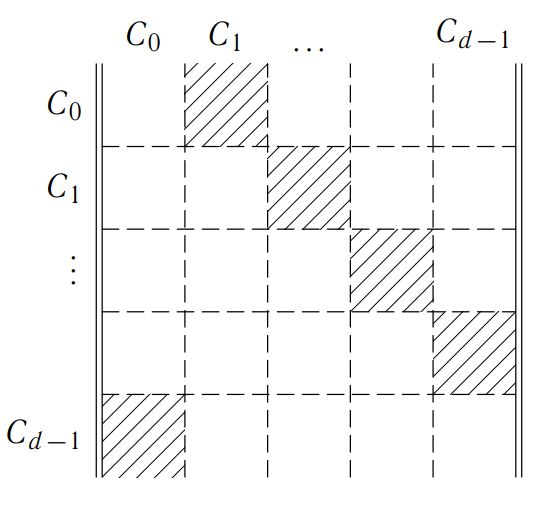
\includegraphics[width=0.3\linewidth]{oduvanchik_i_pic_5.png}
\end{figure}

Предположим сейчас, что блуждающая «частица», эволюция которой
управляется матрицей $\mathbb{P}$, начинает свое движение из некоторого состояния
в подклассе $C_0$. Тогда в каждый из моментов времени $n = p +kd$ эта «частица» будет находиться (в силу определения подклассов $C_0, C_1, \ldots, C_{d-1}$)
в множестве $C_p$.

Следовательно, с каждым таким множеством состояний $C_p$ можно связать \emph{новую} марковскую цепь с матрицей переходов $\Vert {p_{ij}}^{(d)} \Vert$, где $i, j \in C_p$. Эта новая цепь будет \emph{неразложимой} и \emph{апериодической}.

\begin{figure}[h!]
			\centering
			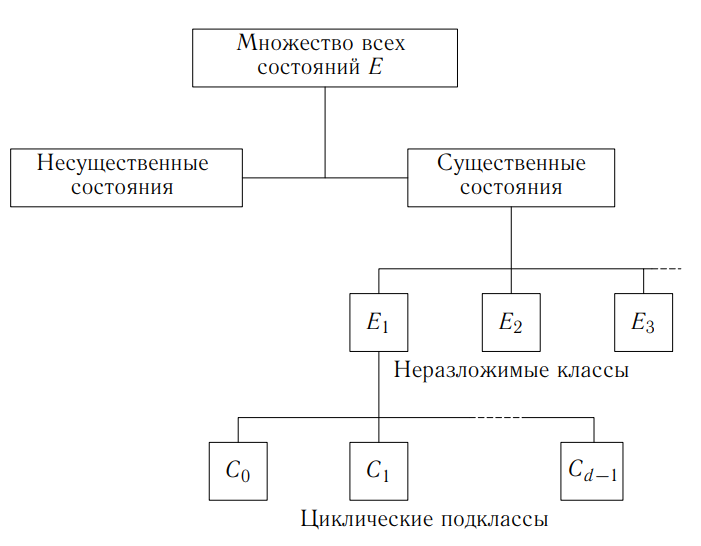
\includegraphics[width=0.6\linewidth]{oduvanchik_i_pic_6.png}
			\caption{Классификация состояний марковской цепи по арифметическим свойствам
вероятностей ${p_{ij}}^{(n)}$}
			\label{ris lab}
\end{figure}

Таким образом, принимая во внимание проведенную классификацию
(на несущественные и существенные состояния, неразложимые классы и
циклические подклассы; см. сводный рис. \ref{fig::oduvan_cycle_motion}), можно сделать такой вывод:

\begin{center}
  При исследовании вопросов предельного поведения переходных вероятностей\\
  ${p_{ij}}^{(n)},~ n \geq 1,~ i,j \in E$, определяющих блуждание «марковской частицы»,\\ можно ограничиваться рассмотрением лишь того случая, когда фазовое\\ пространство $E$ само является \emph{единственным неразложимым апериодическим\\ классом} состояний.
\end{center}

В этом предположении саму марковскую цепь $X = (X_n)_{n \geq 0}$ с таким
фазовым пространством и матрицей переходных вероятностей $\mathbb{P}$ называют
\emph{неразложимой и апериодической}.



\newpage
% Случайные блуждания на конечном множестве с отражающими экранами как марковская цепь

\section{Случайные блуждания на конечном множестве с отражающими экранами как марковская цепь}

\textbf{Автор:} Хайдари Фарид Гулович, Б-01-008

\subsection{Введение}
В данной работе рассматривается представление случайных блужданий на конечном множестве с отражающими экранами в виде марковской цепи. Здесь приводятся свойства данной марковской цепи, такие как периодичность, эргодичность и стационарность, и объясняется, как они связаны с характеристиками случайных блужданий. Также рассматриваются примеры применения марковских цепей в различных областях, таких как физика, экономика и биология, и объясняется, как случайные блуждания могут быть использованы для моделирования различных процессов.

\subsection{О марковских цепях}

\paragraph{Определение}

Одно из свойств, сильно упрощающее исследование случайного процесса — это «марковское свойство». Если объяснять очень неформальным языком, то марковское свойство сообщает нам, что если мы знаем значение, полученное каким-то случайным процессом в заданный момент времени, то не получим никакой дополнительной информации о будущем поведении процесса, собирая другие сведения о его прошлом. Более математическим языком: в любой момент времени условное распределение будущих состояний процесса с заданными текущим и прошлыми состояниями зависит только от текущего состояния, но не от прошлых состояний (\textbf{свойство отсутствия памяти}). Случайный процесс с марковским свойством называется \textbf{марковским процессом}.

$$
\mathbb{P}(\text{будущее} \  | \  \text{настоящее, прошлое}) = \mathbb{P}(\text{будущее} \  | \  \text{настоящее})
$$

Марковское свойство обозначает, что если мы знаем текущее состояние в заданный момент времени, то нам не нужна никакая дополнительная информация о будущем, собираемая из прошлого.

На основании этого определения мы можем сформулировать определение <<однородных цепей Маркова с дискретным временем>> (в дальнейшем для простоты мы их будем называть <<цепями Маркова>>). \textbf{Цепь Маркова} — это марковский процесс с дискретным временем и дискретным пространством состояний. Итак, цепь Маркова — это дискретная последовательность состояний, каждое из которых берётся из дискретного пространства состояний (конечного или бесконечного), удовлетворяющее марковскому свойству.

Рассмотрим цепь Маркова с конечным числом состояний $X = \{1, 2, ..., N\}$. Вероятности
\[
p_{ij}^{(n)} = \mathbb{P} (\xi_{m + n} = j | \xi_m = i), \  n \geq 1, \  m \geq 1, \  i, j \in X
\]
называются вероятностями перехода цепи Маркова за n шагов, а $p_{ij}$ = $p_{ij}$ просто вероятностями перехода. Матрица вида
\[
P = \begin{pmatrix}
p_{11} & p_{12} & \dots & p_{1N}\\
p_{21} & p_{22} & \dots & p_{2N}\\
\vdots & \vdots & \ddots & \vdots\\
p_{N1} & p_{N2} & \dots & p_{NN}
\end{pmatrix}
\]
называется матрицей вероятностей перехода цепи Маркова.

\paragraph{Свойства}

В данном разделе доклада мы рассмотрим свойства марковских цепей, в частности, свойства разложимости, апериодичности и возвратности. Неразложимость цепи Маркова означает, что из любого состояния можно достичь любого другого состояния с ненулевой вероятностью. Апериодичное состояние имеет период $d$, если для возврата в это состояние нужно количество этапов времени, кратное $d$, и является апериодическим, если апериодичны все её состояния. Невозвратное состояние имеет ненулевую вероятность того, что мы никогда в него не вернёмся, а возвратное состояние означает, что мы можем вернуться в него с вероятностью 1. Для возвратных состояний можно вычислить ожидаемое время возврата, которое может быть как конечным, так и бесконечным. В следующих разделах мы рассмотрим некоторые теоремы, связанные с марковскими цепями, и применения марковских цепей в различных областях.

\paragraph{Разложимость}

\textbf{Несущественным состоянием} $i \in X$ называется состояние, из которого можно за положительное число шагов выйти: $\exists m, j : p_{ij} > 0$, но нельзя в него вернуться: $\forall n : p_{ij} = 0$.

Если из множества $X$ всех состояний выделить несущественные, то оставшееся множество \textbf{существенных} состояний обладает тем свойством, что, попав в него, цепь Маркова никогда из него не выйдет.

\textbf{Сообщающимися состояниями} $i$ и $j$ называются существенные состояния, если $i$ достижимо из $j$, и $j$ достижимо из $i$ с ненулевой вероятностью. Обозначается как $i \leftrightarrow j$.

Множество существенных состояний разбивается на конечное или счетное число непересекающихся множеств $X_1 , X_2 , ...$ состоящих из сообщающихся состояний и характеризующихся тем, что переходы между различными множествами невозможны. Тогда такие множества называют \textbf{классами} или \textbf{неразложимыми классами} существенных сообщающихся состояний.

Цепь Маркова \textbf{неразложима}, если можно достичь любого состояния из любого другого состояния с ненулевой вероятностью (необязательно, что за один шаг времени). Если пространство состояний конечно и цепь можно представить в виде графа, то мы можем сказать, что граф неразложимой цепи Маркова сильно связный.
\begin{figure}[H]
    \centering
    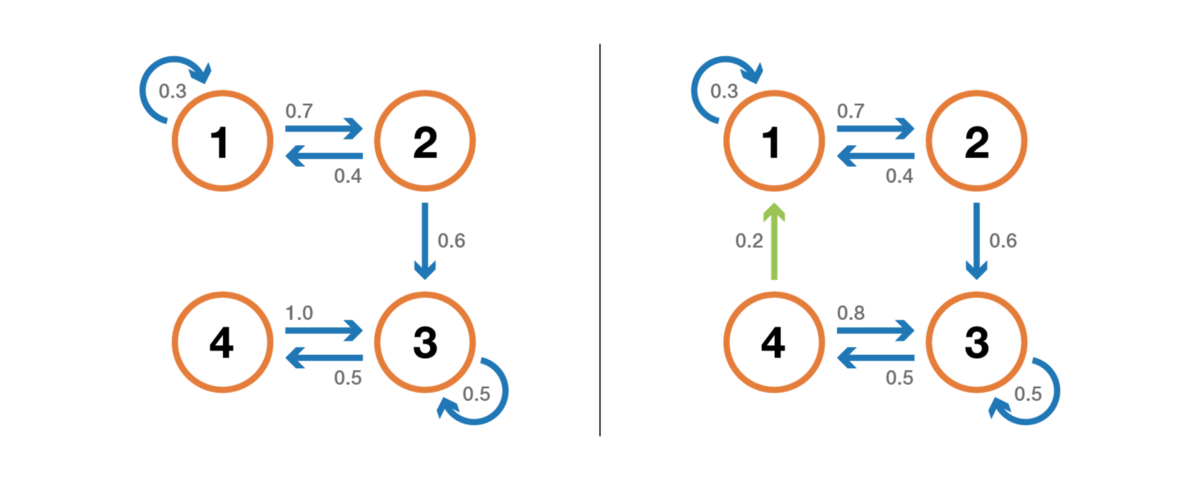
\includegraphics[width=0.6\textwidth]{fscanf_pic_razloshimost.png}
    \caption{Иллюстрация свойства неразложимости (несокращаемости). Цепь слева нельзя сократить: из $3$ или $4$ мы не можем попасть в $1$ или $2$. Цепь справа (добавлено одно ребро) можно сократить: каждого состояния можно достичь из любого другого с ненулевой вероятностью.}
\end{figure}

\paragraph{Апериодичность}

Состояние имеет период $d$, если при уходе из него для любого возврата в это состояние нужно количество этапов времени, кратное $d$ ($d$ -- наибольший общий делитель всех возможных длин путей возврата). Если $d = 1$, то говорят, что состояние является апериодическим, а вся цепь Маркова является \textbf{апериодической}, если апериодичны все её состояния. В случае неприводимой цепи Маркова можно также упомянуть, что если одно состояние апериодическое, то и все другие тоже являются апериодическими.
\begin{figure}[H]
    \centering
    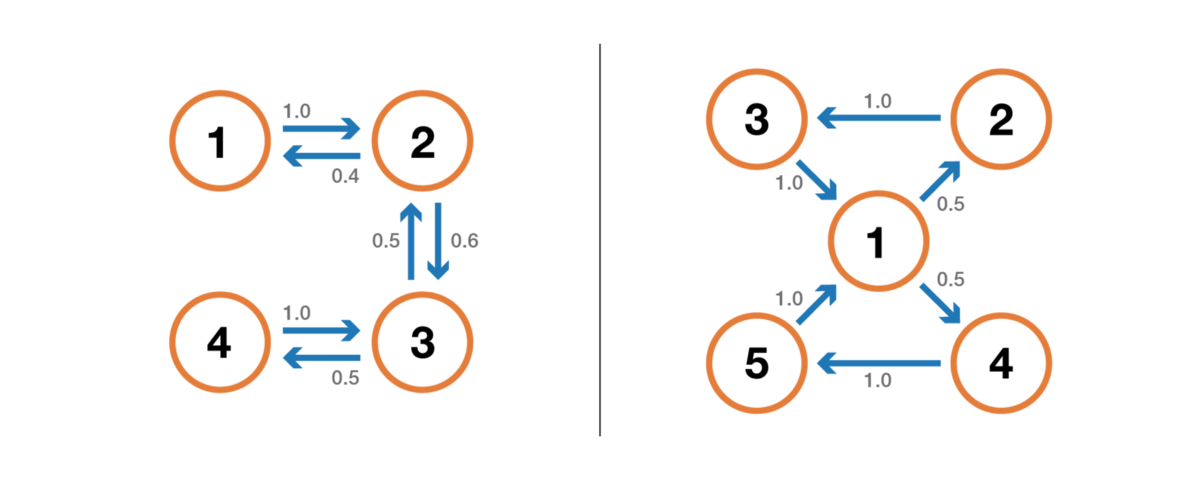
\includegraphics[width=0.6\textwidth]{fscanf_pic_aperiodichnost.png}
    \caption{Иллюстрация свойства периодичности. Цепь слева периодична с $d = 2$: при уходе из любого состояния для возврата в него всегда требуется количество шагов, кратное $2$. Цепь справа имеет период $3$}
\end{figure}

\paragraph{Возвратность}
Состояние является \textbf{невозвратным}, если при уходе из состояния существует ненулевая вероятность того, что мы никогда в него не вернёмся. И наоборот, состояние считается \textbf{возвратным}, если мы знаем, что после ухода из состояния можем в будущем вернуться в него с вероятностью 1 (если оно не является невозвратным).
\begin{figure}[H]
    \centering
    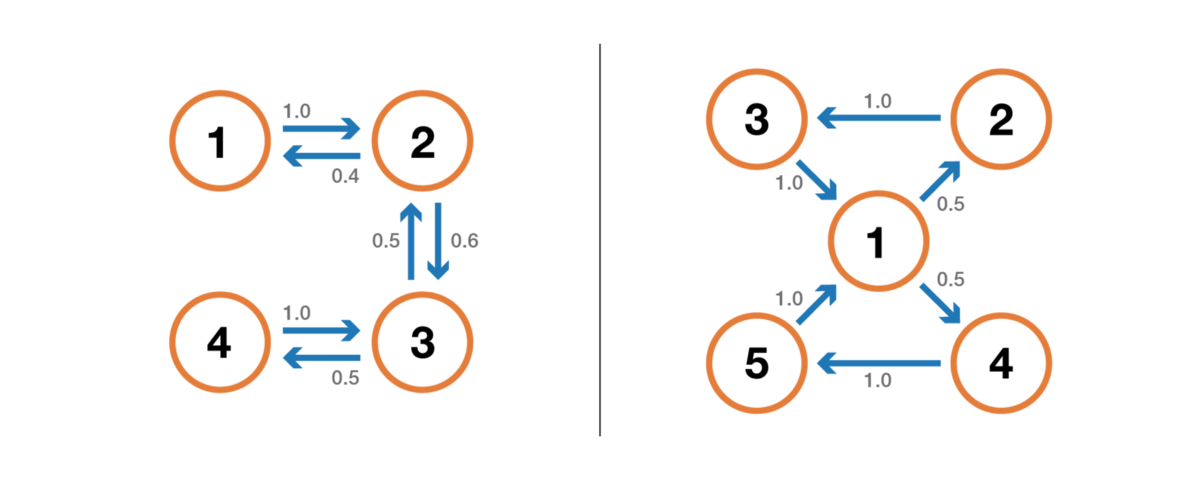
\includegraphics[width=0.6\textwidth]{fscanf_pic_aperiodichnost.png}
    \caption{Иллюстрация свойства возвратности/невозвратности. Цепь слева имеет такие свойства: $1$, $2$ и $3$ невозвратны (при уходе из этих точек мы не можем быть абсолютно уверены, что вернёмся в них) и имеют период $3$, а $4$ и $5$ возвратны (при уходе из этих точек мы абсолютно уверены, что когда-нибудь к ним вернёмся) и имеют период $2$. Цепь справа имеет ещё одно ребро, делающее всю цепь возвратной и апериодической.}
\end{figure}

Для возвратного состояния мы можем вычислить среднее время возвратности, которое является \textbf{ожидаемым временем возврата} при покидании состояния. Заметьте, что даже вероятность возврата равна $1$, то это не значит, что ожидаемое время возврата конечно. Поэтому среди всех возвратных состояний мы можем различать \textbf{положительные возвратные состояния} (с конечным ожидаемым временем возврата) и \textbf{нулевые возвратные состояния} (с бесконечным ожидаемым временем возврата).

\paragraph{Характеристики динамики, описываемой цепью Маркова}

Данный раздел доклада посвящен характеристикам динамики, описываемой цепью Маркова. В этом разделе мы рассмотрим три ключевых понятия: стационарное распределение, предельное распределение и эргодичность. Стационарное распределение является таким распределением вероятностей, которое не изменяется со временем. Предельное распределение является стационарным распределением для положительно возвратной и апериодической цепи Маркова. Эргодичность связана с поведением цепи Маркова и говорит нам, что в пределе ранее поведение траектории становится несущественным, и при вычислении временного среднего важно только долговременное стационарное поведение. В данном разделе мы рассмотрим каждое из этих понятий более подробно, включая определение и примеры.

\paragraph{Стационарное распределение}

Распределение вероятностей $\pi$ по пространству состояний $E$ называют \textbf{стационарным распределением}, если оно удовлетворяет выражению
\[
\pi_i = \sum_{j \in E} \pi_j p_{ji}, \  \forall i \in E
\]
Левая часть -- вероятность нахождения в состоянии $e'$ на текущем шагу, правая -- вероятность перехода в состояние $i$ на следующем шагу.

По определению, стационарное распределение вероятностей со временем не изменяется. То есть если исходное распределение является стационарным, тогда оно будет одинаковых на всех последующих этапах времени. Если пространство состояний конечно, то $p$ можно представить в виде матрицы $P$, а $\pi$ — в виде вектора-строки, и тогда мы получим
$$ \pi = \pi P = \pi P^2 = ... $$

Это снова выражает тот факт, что стационарное распределение вероятностей со временем не меняется (умножение справа распределения вероятностей на $P$ позволяет вычислить распределение вероятностей на следующем этапе времени). Неразложимая цепь Маркова имеет стационарное распределение вероятностей тогда и только тогда, когда одно из её состояний является положительным возвратным.

\paragraph{Предельное распределение}

Если цепь является положительной возвратной (то есть в ней существует стационарное распределение) и апериодической, тогда, какими бы ни были исходные вероятности, распределение вероятностей цепи сходится при стремлении интервалов времени к бесконечности: говорят, что цепь имеет \textbf{предельное распределение}, что является ничем иным, как стационарным распределением. В общем случае его можно записать так:
\[
\lim_{n \to \infty} \mathbb{P} (X_n = i \  | \  X_0 = j) = \lim_{n \to \infty} p_{ij}^n = \pi_i, \  \forall (i, j) \in E \times E
\]

Мы не делаем никаких допущений об исходном распределении вероятностей: распределение вероятностей цепи сводится к стационарному распределению (равновесному распределению цепи) вне зависимости от исходных параметров.

\paragraph{Эргодичность}

\textbf{Эргодичность} — это свойство, связанное с поведением цепи Маркова. Если цепь Маркова неразложима, то также говорится, что она <<эргодическая>>, потому что удовлетворяет следующей эргодической теореме. Допустим, у нас есть функция $f(.)$, идущая от пространства состояний $E$ к оси (это может быть, например, цена нахождения в каждом состоянии). Мы можем определить среднее значение, перемещающее эту функцию вдоль заданной траектории (временное среднее). Для $n$-ных первых членов это обозначается как
\[
\frac{1}{n} ( f(X_0) + f(X_1) + ... + f(X_{n - 1} ) = \frac{1}{n} \sum_{i = 0}^{n - 1} f(X_i)
\]
Также мы можем вычислить среднее значение функции $f$ на множестве $E$, взвешенное по стационарному распределению (пространственное среднее), которое обозначается
\[
\sum_{i \in E} \pi_i f_i
\]

Тогда эргодическая теорема говорит нам, что когда траектория становится бесконечно длинной, временное среднее равно пространственному среднему (взвешенному по стационарному распределению). Свойство эргодичности можно записать так:
\[
\lim_{n \to \infty} \frac{1}{n} \sum_{i = 0}^{n - 1} f(X_i) = \sum_{e \in E} \pi(e) f(e)
\]
Иными словами, оно обозначает, что в пределе ранее поведение траектории становится несущественным и при вычислении временного среднего важно только долговременное стационарное поведение.

\paragraph{Некоторые теоремы}

\begin{theorem}\label{th1}

Рассматривается марковская цепь со счетным множеством состояний $E = \{1,2, ...\}$ такая, что ее переходные вероятности $p_{ij}, i, j \in E$, таковы, что существуют пределы
$$
\pi_j = \lim_n p_{ij}^{(n)}, \  j \in E
$$
не зависящие от начальных состояний $i \in E$. Тогда
\begin{enumerate}[label=(\alph*)]
    \item $\sum\limits_{j = 1}^{\infty} \pi_j \leq 1, \sum\limits_{j = 1}^{\infty} \pi_i p_{ij} = \pi_j, j \in E$
    \item имеет место альтернатива: либо $\sum\limits_{j = 1}^{\infty} \pi_j = 0$ (и, значит, все $\pi_j = 0, j \in E$, либо $\sum\limits_{j = 1}^{\infty} \pi_j = 1$
    \item если $\sum\limits_{j = 1}^{\infty} \pi_j = 0$, то у марковской цепи отсутствуют стационарные распределения; если же $\sum\limits_{j = 1}^{\infty} \pi_j = 1$ то вектор предельных значений $\Pi = (\pi_1, \pi_2, ...)$ образует для этой цепи стационарное распределение и других стационарных распределений у этой цепи уже не существует.
\end{enumerate}

\begin{proof}

Имеем
\begin{equation}\label{eq1}
\sum_{j = 1}^{\infty} \pi_j = \sum_{j = 1}^{\infty} \lim_n p_{ij}^{(n)} \leq \varliminf_n \sum_{j = 1}^{\infty} p_{ij}^{(n)} = 1
\end{equation}
и для любых $j \in E, k \in E$
\begin{equation}\label{eq2}
\sum_{j = 1}^{\infty} \pi_j p_{ij} = \sum_{j = 1}^{\infty} \lim_n p_{ij}^{(n)} p_{ij} \leq \varliminf_n \sum_{j = 1}^{\infty} p_{ij}^{(n)} p_{ij} = \varliminf_n p_{kj}^{(n + 1)} = \pi_j
\end{equation}
Итак, вектор предельных вероятностей $\Pi = (\pi_1, \pi_2, ...)$ обладает следующими свойствами:
\begin{equation}\label{eq3}
\sum_{j = 1}^{\infty} \pi_j \leq 1 \text{ и } \sum_{i = 1}^{\infty} \pi_i p_{ij} \leq \pi_j, j \in E
\end{equation}
Покажем, что в последнем неравенстве на самом деле имеет место равенство.

Пусть для некоторого $j_0 \in E$
\begin{equation}\label{eq4}
\sum_{i = 1}^{\infty} \pi_i p_{i j_0} < \pi_{j_0}
\end{equation}
Тогда
$$
\sum_{j = 1}^{\infty} \pi_j > \sum_{j = 1}^{\infty} \left( \sum_{i = 1}^{\infty} \pi_i p_{ij} \right) = \sum_{i = 1}^{\infty} \pi_i \sum_{j = 1}^{\infty} p_{ij} = \sum_{i = 1}^{\infty} \pi_i.
$$
Полученное противоречие показывает, что $\sum\limits_{i = 1}^{\infty} \pi_i p_{ij} = \pi_j$ итерациями получаем, что для любого $n \geq 1$ и любого $j \in E$
$$
\sum_{i = 1}^{\infty} \pi_i p_{ij}^{(n)} = \pi_j
$$
Отсюда по теореме Лебега о мажорируемой сходимости
$$
\pi_j = \lim_n \sum_{i = 1}^{\infty} \pi_i p_{ij}^{(n)} = \sum_{i = 1}^{\infty} \pi_i \lim_n p_{ij}^{(n)} = \left( \sum_{i = 1}^{\infty} \pi_i \right) \pi_j.
$$
т.е.
$$
\pi_j \left( 1 - \sum_{i = 1}^{\infty} \pi_i \right) = 0, \  j \in E
$$
и, значит, $\left( \sum\limits_{j = 1}^{\infty} \pi_j \right) \left( 1 - \sum_{i = 1}^{\infty} \pi_i \right) = 0$. Так что $a (1 - a) = 0$ с $a = \sum\limits_{i = 1}^{\infty} \pi_i$, и поэтому или $a = 1$, или $a = 0$, 0, что и доказывает утверждение (b).

Для доказательства (c) предположим, что $\mathbb{Q} = (q_1, q_2, ...)$ -- какое-то стационарное распределение. Тогда $\sum\limits_{i = 1}^{\infty} q_i p_{ij} = q_j$ и по теореме о мажорируемой сходимости $\left( \sum\limits_{i = 1}^{\infty} q_i \right) \pi_j = q_j, \  j \in E$.

Поэтому, если $\mathbb{Q}$ — стационарное распределение, то $\sum\limits_{i = 1}^{\infty} q_i = 1$ и, следовательно, необходимым образом это стационарное распределение должнобыть таким, что $q_j = \pi_j$ для всех $j \in E$. Так что если $\sum\limits_{j = 1}^{\infty} \pi_j = 0$, то не может выполняться свойство $\sum\limits_{i = 1}^{\infty} q_i = 1$ и, значит, в этом случае стационарного распределения нет.

Согласно (b), остается еще возможность $\sum\limits_{j = 1}^{\infty} \pi_j = 1$. В этом случае, согласно (a), $\Pi = (\pi_1, \pi_2, ...)$ само является стационарным распределением и из изложенного выше следует, что если $\mathbb{Q}$ -- какое-то другое стационарное распределение, то оно должно совпадать с $\Pi$ что и доказывает единственность стационарного распределения в случае $\sum\limits_{j = 1}^{\infty} \pi_j = 1$.

\end{proof}
\end{theorem}

\begin{theorem}[Основная теорема о стационарных распределениях]\label{th2}
Рассматривается марковская цепь со счетным множеством состояний $E$. Для существования единственного стационарного распределения необходимо и достаточно, чтобы
\begin{enumerate}[label=(\alph*)]
    \item существовал в точности один неразложимый подкласс и
    \item все состояния были положительно возвратны.
\end{enumerate}

\begin{proof}
\textbf{Необходимость}. Пусть рассматриваемая цепь имеет и притом единственное стационарное распределение, которое обозначим $\widetilde{\mathbb{Q}}$. Покажем, что тогда в множестве состояний $E$ должен найтись и притом единственный положительно возвратный подкласс.

Обозначим через $N$ потенциально возможное число таких подклассов ($0 \leq N \leq \infty$).

Пусть $N = 0$ и $j$ -- некоторое состояние из $E$. Поскольку положительно возвратных классов нет, то состояние $j$ может быть или невозвратным, или же нулевым возвратным.

В первом случае из теоремы 2 \S 5 \cite{shir2} следует, что для всех $i \in E$ пределы $\lim\limits_{n} p_{ij}^{(n)}$ существуют и равны нулю.

Но и во втором случае эти пределы также существуют и равны нулю, что следует из свойства (37) в \S 5 \cite{shir2} и того, что $\mu_j = \infty$, поскольку состояние $j$ является нулевым возвратным.

Итак, в случае $N = 0$ пределы $\pi_j = \lim\limits_{n} p_{ij}^{(n)}$ существуют для всех $i, j \in E$ и равны нулю. Поэтому по утверждению (с) теоремы \ref{th1} в этом случае нет стационарных распределений и, следовательно, этот случай $N = 0$ исключается предположением существования стационарного распределения $\widetilde{\mathbb{Q}}$.

Пусть теперь $N = 1$. Обозначим единственный положительно возвратный класс через $C$.

Если период этого класса $d(C) = 1$, то, согласно свойству (26) в теореме 3 \S 5 \cite{shir2},
$$
p_{ij}^{(n)} \rightarrow \mu_j^{-1}, \  n \rightarrow \infty
$$
для всех $i, j \in C$. Если же $j \notin C$, то это состояние невозвратно и тогда по свойству (21) в теореме 2 \S 5 \cite{shir2}
$$
p_{ij}^{(n)} \rightarrow 0, \  n \rightarrow \infty
$$
для всех $i \in E$.

Положим
\begin{equation}\label{eq5}
q_j =
  \begin{cases}
    \mu_j^{-1} (> 0), & \text{если $j \in C$}\\
    0, & \text{если $j \notin C$}\\
  \end{cases} 
\end{equation}
Тогда, поскольку множество $C \neq \varnothing$, то по теореме \ref{th1} набор $\mathbb{Q} = (q_1, q_2, ...)$ образует единственное стационарное распределение, и, следовательно, $\mathbb{Q} = \widetilde{\mathbb{Q}}$.

Предположим теперь, что период $d(C) > 1$.

Пусть $C_0, C_1, ..., C_{d-1}$ -- циклические подклассы (положительно возвратного) класса $C$. Относительно матрицы переходных вероятностей $p_{ij}^{(d)}, i, j \in C$, каждый из подклассов $C_k, k = 0, 1, ..., d - 1$, является возвратным и апериодическим. Тогда, если $i, j \in C_k$, то, согласно формуле (36) из \S 5 \cite{shir2},
$$
p_{ij}^{(nd)} \rightarrow \frac{d}{\mu_j} > 0.
$$
Поэтому на каждом множестве $C_k$ набор $\{d / \mu_j, j \in C_k\}$ образует 
(относительно матрицы $p_{ij}^{(nd)}, i, j \in C$) единственное стационарное распределение в силу свойства (Ь) теоремы \ref{th1}.

Отсюда, в частности, следует, что $\sum\limits_{j \in C_k} \frac{d}{\mu_j} = 1$, т.е. $\sum\limits_{j \in C_k} \frac{1}{\mu_j} = \frac{1}{d}$.

Положим
\begin{equation}\label{eq6}
q_j =
  \begin{cases}
    \mu_j^{-1} (> 0), & j \in C = C_0 + ... + C_{d - 1},\\
    0, & j \notin C,\\
  \end{cases} 
\end{equation}
и покажем, что для исходной цепи набор $\mathbb{Q} = (q_1, q_2, ...)$ образует 
единственное стационарное распределение.

В самом деле, если $i \in C$, то
$$
p_{ii}^{(nd)} = \sum\limits_{j \in C} p_{ij}^{(nd - 1)} p_{ji}.
$$
Тогда, как и в\eqref{eq1}, находим, что
$$
\frac{d}{\mu_i} = \lim_n p_{ii}^{(nd)} \geq \sum_{j \in C} \varliminf_n p_{ij}^{(nd - 1)} p_{ji} = \sum_{j \in C} \frac{d}{\mu_j} p_{ji}
$$
и, значит,
\begin{equation}\label{eq7}
\frac{1}{\mu_i} = \sum_{j \in C} \frac{1}{\mu_j} p_{ji}  
\end{equation}

Но
\begin{equation}\label{eq8}
\sum_{i \in C} \frac{1}{\mu_i} = \sum_{k = 0}^{d - 1} \left( \sum_{i \in C_k} \frac{1}{\mu_i} \right) = \sum_{k = 0}^{d - 1} \frac{1}{d} = 1
\end{equation}
Так же, как и в доказательстве теоремы \ref{th1} (см. \eqref{eq3} и \eqref{eq4}), из \eqref{eq7} и \eqref{eq8} выводится, что на самом деле в \eqref{eq7} имеет место знак равенства:
\begin{equation}\label{eq9}
\frac{1}{\mu_i} = \sum_{j \in C} \frac{1}{\mu_j} p_{ji}.
\end{equation}

Поскольку $q_i = \mu_i^{-1} > 0$, то \eqref{eq9} показывает, что набор $\mathbb{Q} = (q_1, q_2, ...)$ образует стационарное распределение, в силу теоремы 1 единственное. Следовательно, $\mathbb{Q} = \widetilde{\mathbb{Q}}$.

Пусть, наконец, $2 < N < \infty$ или $N = \infty$. Обозначим соответствующие положительно возвратные подклассы через $C^1, ..., C^N$, если $N < \infty$, и $C^1, C^2, ...$, если $N = \infty$.

Пусть $\mathbb{Q}^k = (q_1^k, q_2^k, ...)$ -- стационарное распределение для класса $C^k$ построенное по формуле (ср. с  \eqref{eq5}, \eqref{eq6})
$$
q_j^k =
  \begin{cases}
    \mu_j^{-1} (> 0), & j \in C^k,\\
    0, & j \notin C,\\
  \end{cases} 
$$
Тогда для любых неотрицательных чисел $a_1, a_2, ...$ таких, что $\sum_{k = 1}^{\infty} a_k = 1$ ($a_{N + 1} = ... = 0$, если $N < \infty$), набор $a_1 \mathbb{Q}^1 + ... + a_N \mathbb{Q}^N + ...$ будет, очевидно, образовывать стационарное распределение. Тем самым допущение $2 \leq N \leq \infty$ приводит к существованию континуума стационарных распределений, что противоречит сделанному предположению о единственности стационарного распределения.

Итак, проведенное доказательство показывает, что возможен лишь случай $N = 1$. Иначе говоря, существование (единственного) стационарного распределения влечет наличие у цепи в точности одного неразложимого класса, состоящего из положительно возвратных состояний.

\textbf{Достаточность}. Если у цепи существует неразложимый подкласс положительно возвратных состояний, т.е. имеет место случай $N = 1$, то тогда из предшествующих рассмотрений вытекают в силу утверждения (c) теоремы \ref{th1} и существование, и единственность стационарного распределения.

\end{proof}
\end{theorem}

\begin{theorem}[Основная теорема об эргодических распределениях]\label{th3}
Рассматривается марковская цепь со счетным множеством состояний. Для существования эргодического распределения необходимо и достаточно, чтобы цепь являлась
\begin{enumerate}[label=(\alph*)]
    \item неразложимой,
    \item положительно возвратной и
    \item апериодической.
\end{enumerate}

\begin{proof}

\textbf{Достаточность}. Если пользоваться обозначениями из доказательства теоремы \ref{th2}, то по условиям теоремы мы имеем $N = 1$, $C = E$ и $d(E) = 1$ (апериодичность). Тогда из рассмотрений <<случая $N = 1$>> в доказательстве теоремы \ref{th2} следует, что набор $\mathbb{Q} = (q_1, q_2, ...)$ с $q_j = \mu_j^{-1}, j \in E$, образует одновременно стационарное и эргодическое распределение, поскольку все $\mu_j^{-1}, j \in E$.

Итак, существование эргодического распределения $\Pi = (\pi_1, \pi_2, ...)$ установлено ($\Pi = \mathbb{Q}$).

\textbf{Необходимость}. Если существует эргодическое распределение $\Pi = (\pi_1, \pi_2, ...)$, то, согласно теореме \ref{th1}, существует и единственно  стационарное распределение $\mathbb{Q}$, совпадающее с $\Pi$.

Из утверждения теоремы \ref{th2} (и ее доказательства) следует, что случаи $N = 0$ и $2 \leq N \leq \infty$ не могут реализоваться, и, значит, $N = 1$ и существует лишь один неразложимый класс $C$, состоящий из положительно возвратных состояний. Все, что осталось сделать, так это показать, что $C = E$ и $d(E) = 1$.

Если предположить, что $C \neq E$ и $d(C) = 1$, то опять же из рассмотрения <<случая $N = 1$>> в доказательстве теоремы \ref{th2} вытекало бы, что существует состояние $j \notin C$ такое, что $p_{ij}^{(n)}$ для всех $i \in E$. Это, однако, вступает в противоречие с тем, что $\pi_j = \lim\limits_n p_{ij}^{(n)} > 0$ для всех $i \in E$.

Таким образом, в случае $d(C) = 1$ имеем $C = E$ и $d(E) = 1$ (апериодичность).

Наконец, если $C \neq E$ и $d(C) > 1$, то опять же из рассмотрений <<случая $N = 1$>> в теореме \ref{th2} следует, что тогда имеется стационарное распределение $\mathbb{Q} = (q_1, q_2, ...)$, у которого некоторые $q_j= 0$, что противоречит тому, что $\mathbb{Q} = \Pi$, а $\Pi = (\pi_1, \pi_2, ...)$ -- эргодическое распределение, у которого (по определению) все $\pi_j > 0$, $j \in E$.

\end{proof}
\end{theorem}


\paragraph{Случайные блуждания на конечном множестве с отражающими экранами как марковская цепь}

\paragraph{Теория}

Рассматривается простое случайное блуждание с двумя \textit{отражающими} экранами в точках $0$ и $N$:
\begin{figure}[H]
    \centering
    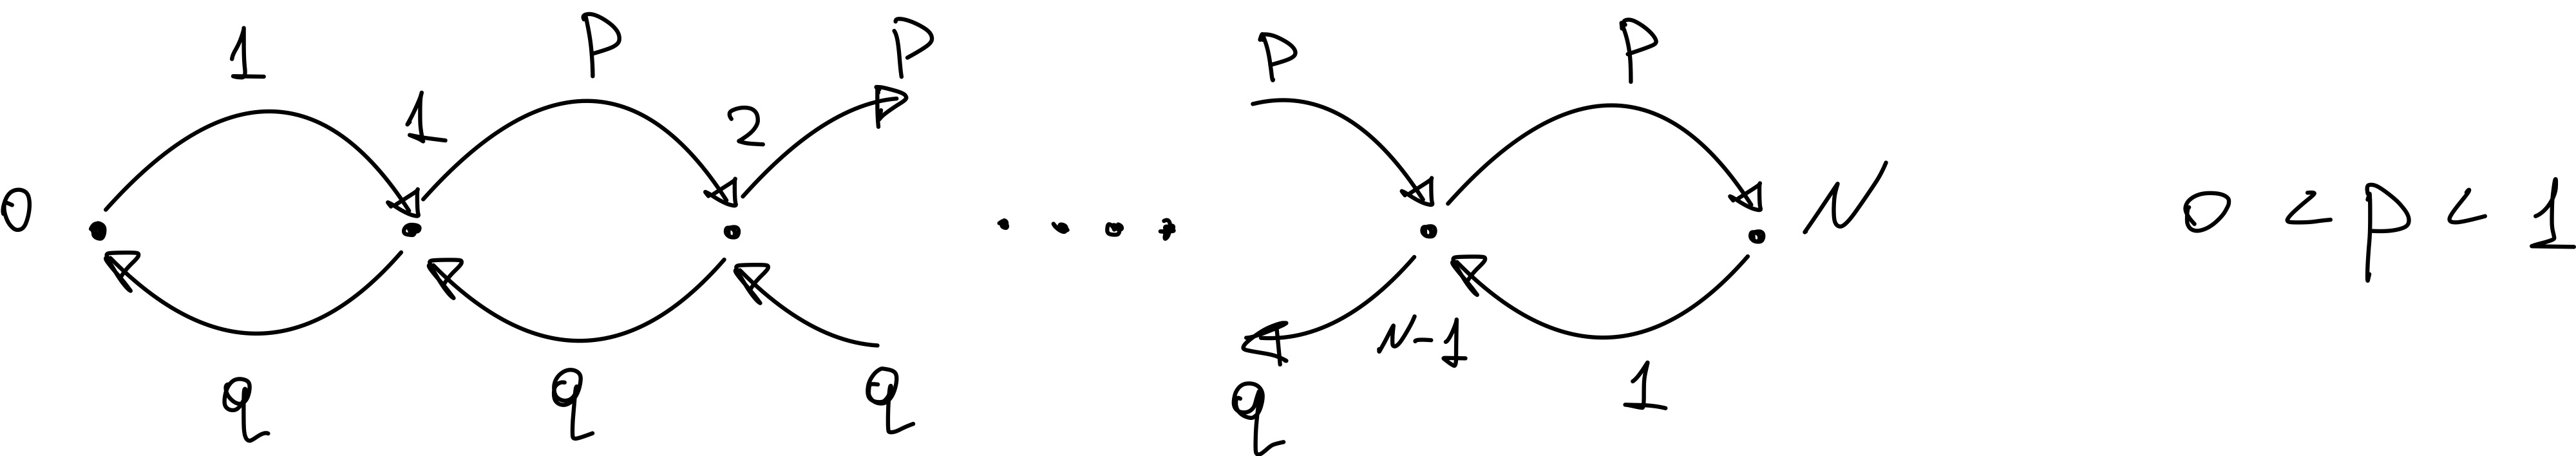
\includegraphics[width=0.8\textwidth]{fscanf_pic_bluzhdanie.JPG}
\end{figure}

Состояния цепи образуют здесь один неразложимый класс. Они  являются положительно возвратными с периодом $d = 2$. Из основной теоремы о стационарных распределениях (теорема \ref{th2}), у рассматриваемой цепи \textit{существует} и \textit{единственно} стационарное распределение $\mathbb{Q} = \{ q_0, q_1, ..., q_N \}$. Решая систему уравнений $q_j = \sum_{i = 0}^N q_i p_{ij}$ с условием $\sum_{i = 0}^N q_i = 1, \  q_i \geq 0, \  j \in E $, находим, что:
\begin{equation}\label{pi_i}
q_j = \frac{ \left( \frac{p}{q} \right)^{j - 1} }{1 + \sum_{j = 1}^{N - 1} \left( \frac{p}{q} \right)^{j - 1} }, \  2 \leq j \leq N - 1
\end{equation}
и $q_0 = q_1 q$, $q_N = q_{N - 1} p$.

Эргодическое распределение отсутствует -- это следует из основной теоремы об эргодических распределениях (теорема \ref{th3}) и того факта, что у рассматриваемой цепи период $d = 2$. Можно и непосредственно убедиться в том, что здесь нет эргодического распределения. Пусть, например, $N = 2$:
\begin{figure}[H]
    \centering
    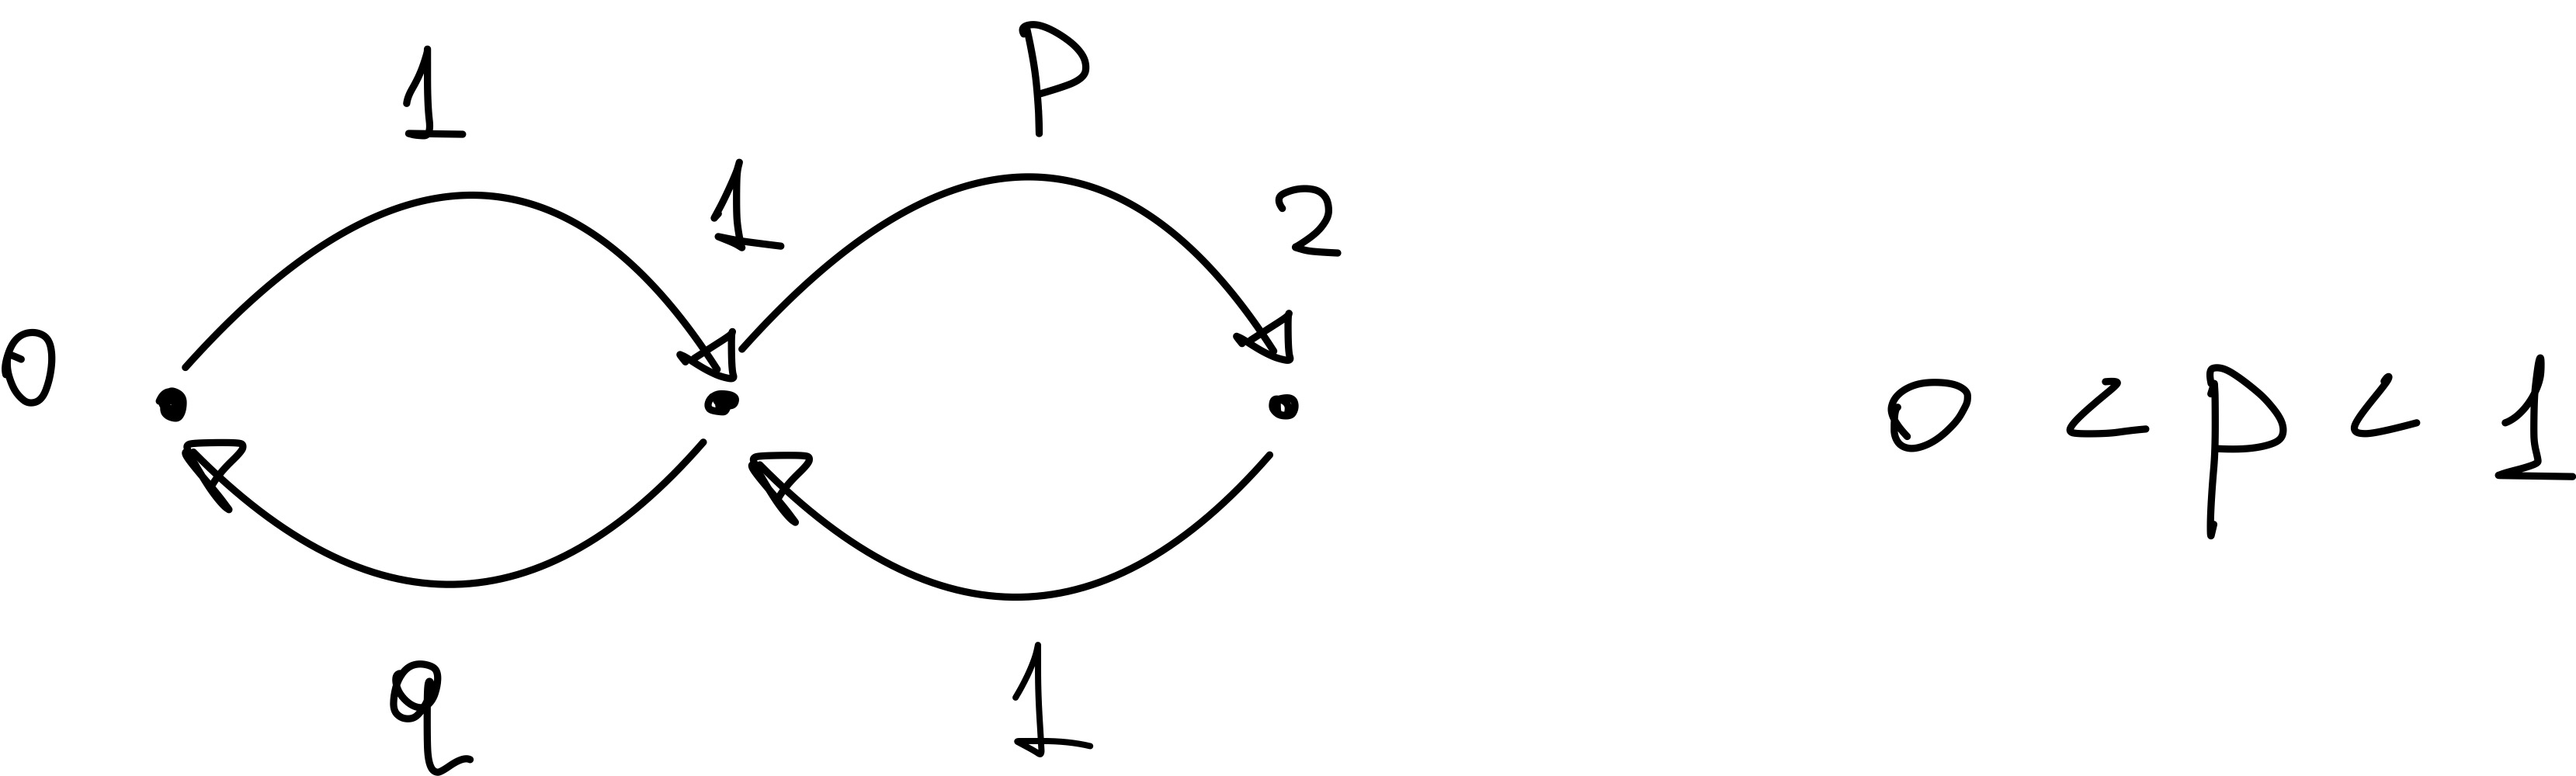
\includegraphics[width=0.5\textwidth]{fscanf_pic_bluzhdanie2.JPG}
\end{figure}

Тогда видно, что $p_{11}^{2n} = 1$, но $p_{11}^{2n + 1} = 0$. Так что $\lim_n p_{11}^{(n)}$ не существует. В то же самое время стационарное распределение \[ \mathbb{Q} = (q_0, q_1, q_2) \] есть, и, как следует из \eqref{pi_i}, оно имеет вид:
$$
q_0 = \frac{1}{2} q, \  q_1 = \frac{1}{2}, \  q_2 = \frac{1}{2} p
$$

\paragraph{Примеры применения}

Случайные блуждания на конечном множестве с отражающими экранами находят применение в различных областях, включая физику, экономику и теорию управления.

Один из примеров -- моделирование диффузии в физике. В этом случае цепь Маркова описывает движение частиц в системе, где отражающие экраны соответствуют границам реактора. Моделирование такого процесса позволяет оценить, как быстро распространяются частицы и как они взаимодействуют друг с другом.

В экономике случайные блуждания могут использоваться для моделирования цен на акции или валютные курсы. В этом случае цепь Маркова описывает изменение цен на основе предыдущих значений. Это позволяет анализировать поведение рынка и прогнозировать будущие цены.

В теории управления случайные блуждания используются для моделирования процессов принятия решений. Например, можно использовать цепь Маркова для моделирования процесса выбора определенной стратегии в зависимости от предыдущих решений. Это может помочь определить оптимальную стратегию и принять решение на основе вероятностных расчетов.

Таким образом, случайные блуждания на конечном множестве с отражающими экранами являются важным инструментом для моделирования случайных процессов в различных областях. Изучение свойств и теорем, связанных с цепями Маркова, позволяет более глубоко понимать эти процессы и использовать их для прогнозирования и принятия решений.

\paragraph{Заключение}

Случайные блуждания на конечном множестве с отражающими экранами -- это важный инструмент для моделирования случайных процессов в различных областях, таких как физика, экономика и теория управления. В физике они используются для моделирования диффузии частиц, а в экономике - для прогнозирования цен на акции или валютные курсы. В теории управления они помогают определить оптимальную стратегию и принять решение на основе вероятностных расчетов.

Изучение свойств и теорем, связанных с цепями Маркова, позволяет более глубоко понимать эти процессы и использовать их для прогнозирования и принятия решений. Важно отметить, что при моделировании случайных процессов необходимо учитывать все возможные факторы, которые могут повлиять на результаты. Также необходимо оценивать точность моделирования и корректировать ее при необходимости.

В целом, случайные блуждания на конечном множестве с отражающими экранами - это мощный инструмент для анализа случайных процессов. Их применение в различных областях позволяет получать более точные прогнозы и принимать более обоснованные решения.



\newpage
% Одномерная функция распределения 

\section{Одномерная функция распределения случайной величины}

\textbf{Автор:} Полешко Анастасия Олеговна, Б-01-006

Одномерная функция распределения непрерывной случайной величины (CDF - от англ. Cumulative Distribution Function) задает вероятность того, что случайная величина $X$ примет значение меньше или равное $x$. Функция CDF обычно обозначается как $F_X(x)$ или просто $F(x)$.

Для непрерывной случайной величины $X$ функция распределения определяется следующим образом:

$$F_{\xi} (x) = P(X \leq x) = \int_{- \infty}^{\xi} f_{X}(t)dt$$

где $f_X(x)$ - плотность распределения непрерывной случайной величины $X$.

Свойства функции распределения непрерывной случайной величины: 

1. Функция распределения неубывающая: $F(x_1) \leq F(x_2)$, если $x_1 \leq x_2$.

2. Функция распределения ограничена: $0\leq F(x) \leq 1$ для всех $x$.

3. Функция распределения непрерывна справа: $\lim_{\epsilon \to +0} F(x + \epsilon) = F(x)$ для всех $x$.

4. Функция распределения имеет предел при $x\to -\infty$: $\lim_{x\to -\infty} F(x) = 0$.

5. Функция распределения имеет предел при $x\to +\infty$: $\lim_{x\to +\infty} F(x) = 1$.

Используя функцию распределения непрерывной случайной величины можно находить вероятности попадания случайной величины в интервалы, выражать их в виде интегралов и решать задачи на нахождение квантилей и моментов случайной величины.$^{\text{\cite{ShiryaevVeroyatnost1}}}$

Мы будем изучать непрерывные процессы, а потом их дискретизировать с помощью теоремы Котельникова. $^{\text{\cite{ShamarovDRP}, Лекция №1}}$

Рассмотрим теперь случай дискретной случаной величины.
 
Пусть $(\Omega, \varkappa, \mathbb{P})$ -- вероятностная модель некоторого эксперимента с конечным числом исходов $N(\Omega)$ и алгеброй  всех подмножеств П в $\Omega$, где 

$\Omega$ -- произвольное непустое множество, элементы которого называются элементарными событиями, исходами или точками;

$\varkappa$ --  сигма-алгебра подмножеств 
$\Omega$ , называемых случайными событиями;

$\mathbb{P}$ -- вероятностная мера или вероятность, то есть сигма-аддитивная конечная мера, такая что
$\mathbb{P}(\Omega) = 1.$

$N(\Omega)$ -- мощность множества $\Omega$ для случайной величины.

Вводимое сейчас (и далее — в более общем виде) понятие случайной величины призвано определить величины, характеризующие результаты «измерений» в случайных экспериментах.

\begin{definition}\label{poleshko_def_1} Всякая числовая функция $\xi = \xi(w)$, определенная на пространстве элементарных событий $\Omega$, будет называться случайной величиной.
	\end{definition}

\begin{definition}\label{poleshko_def_2} Всякая числовая функция $\xi = \xi(w)$, определенная на конечном пространстве элементарных событий $\Omega$, будет называться простой случайной величиной.
	\end{definition}

\begin{example} В модели двукратного подбрасывания монеты с пространством исходов П = {ГГ, ГР, РГ, РР} определим случайную величину $\xi = \xi(w)$ с помощью таблицы

\begin{center}
\begin{tabular}{ | c | c | c | c | c |}
\hline
w & ГГ & ГР  & РГ & РР\\ \hline
$\xi(w)$ & 2 & 1  & 1 & 0\\ \hline
 \end{tabular}
\end {center}

Здесь $\xi(w)$ по своему смыслу есть не что иное, как число «гербов», отвечающее исходу w.
\end{example}

Другим простейшим примером случайной величины $\xi$ является характеристическая функция некоторого множества $A \in \varkappa$:

\begin{center}

$\xi = I_A(w)$, где

\begin{equation*}
I_A(w) = 
 \begin{cases}
   1 &\text{ $w\in A$}\\
   0 &\text{ $w \notin A$}
 \end{cases}
\end{equation*}

\end{center}

Когда экспериментатор имеет дело со случайными величинами, описывающими те или иные показания, то основной вопрос, который его интересует, — это вопрос о том, с какими вероятностями эта случайная величина принимает те или иные значения. С этой точки зрения интерес представляет не распределение вероятностей Р на $(\Omega, \varkappa)$, а распределение вероятностей на множестве значений случайной величины. Поскольку в рассматриваемом случае $\Omega$ состоит из конечного числа точек, то множество значений X случайной величины $\xi$ также конечно. Пусть $X = {x_1, ..., x_m}$, где (различными) числами $x_1, ..., x_m$ исчерпываются все значения $\xi$.

Обозначим $\chi$ -- совокупность всех подмножеств множества X, и пусть $B \in \chi$ . Множество В можно также интерпретировать как некоторое событие, когда пространство исходов есть X -- множество значений $\xi$.
Рассмотрим на $(X, \chi )$ вероятность $Р_{\xi}(\cdot)$, индуцируемую случайной величиной $\xi$ по формуле

$$P_{\xi} (B) = P\{ w: \xi(w) \in B\}, \ \ \ \ \ B \in \chi$$.

Ясно, что значения этих вероятностей полностью определяются вероятностями

$$P_{\xi} (x_i) = P\{ w: \xi(w) = x_i\}, \ \ \ \ \ x_i \in X$$.

Набор чисел $\{ P_{\xi} (x_1), ..., P_{\xi} (x_m)\}$ называется распределением вероятностей случайной величины $\xi$.

\begin{example} Случайная величина $\xi$, принимающая два значения 1 и О с вероятностями («успеха») р и («неуспеха») q, называется бернуллиевской. Ясно, что для нее

$$P_{\xi} (x) = p^xq^{1-x}, \ \ \ \ \ x = 0, \ 1.$$

Биномиальной (или биномиально распределенной) случайной величиной $\xi$ называется случайная величина, принимающая n + 1 значение 0, 1 , ..., n с вероятностями

$$P_{\xi} (x) = p^xq^{1-x}, \ \ \ \ \ x = 0, \ 1, \ ..., \ n.$$
\end{example}

Заметим, что в этих и во многих приводимых далее примерах мы не конкретизируем структуру основного вероятностного пространства $(\Omega, \varkappa, P)$, а интересуемся лишь значениями случайных величин и их распределениями вероятностей.

Вероятностная структура случайных величин $\xi$ полностью описывается распределением вероятностей $\{ P_{\xi}(x_i), i = 1, ..., m\}$. Вводимое ниже понятие функции распределения дает эквивалентное описание вероятностной структуры случайных величин.

\begin{definition} Пусть $x \in R^1$. Функция

$$F_{\xi}(x) = P\{ w: \xi(w) \leq x\}$$

называется функцией распределения случайной величины $\xi$. 

Ясно, что

$F_{\xi}(x) = \sum\limits_{i: x_i \leq x} P_{\xi}(x_i)$ и $P_{\xi}(x_i) = F_{\xi}(x_i) - F_{\xi}(x_i-0)$, где $F_{\xi}(x_i-0) = \lim\limits_{y \to x-0} F_{\xi}(y)$.

Если считать, что $x_1 < x_2 < ... < x_m$, и положить $F_{\xi}(x_0) = 0$, то

$$P_{\xi}(x_i) = F_{\xi}(x_i) - F_{\xi}(x_i-0), \ \ \ \ \ \ \ i = 1, ..., m$$.

\end{definition}

Приводимые далее графики дают представление о $P_{\xi}(x)$ и $F_{\xi}(x)$ для биномиальной случайной величины $\xi$.

\begin{figure}[h]
    \center 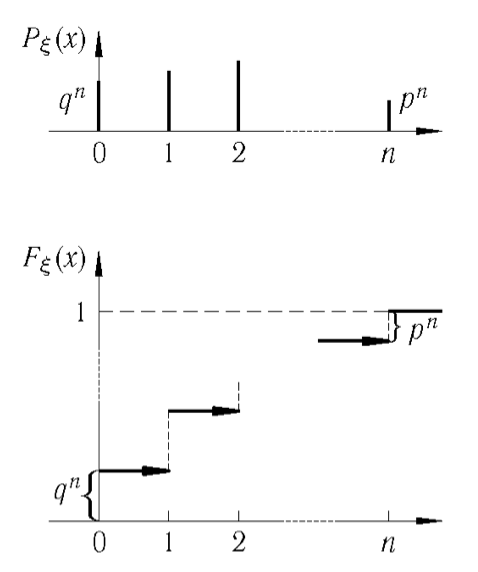
\includegraphics[scale = 0.54]{poleshko02_pic_1.png}
    \label{fig:image}
\end{figure}

Непосредственно из определения \ref{poleshko_def_2} следует, что функция распределения $F_{\xi} = F_{\xi}(x_i)$ обладает такими свойствами: 

(1)$F_{\xi}(- \infty)=0,F_{\xi}(+\infty)= 1$;

(2) $F_{\xi}(x)$ непрерывна справа $F_{\xi}(x+0) = F_{\xi}(x)$ и кусочно постоянна.$^{\text{\cite{ShiryaevVeroyatnost1}}}$


\begin{example} Приведем пример, где рассмотрим функцию распределения случайной величины, как полусумму функции распределения случайной величины, принимающей одно значение и случайной величины с гауссовской плотностью. И покажем, что эта случайная величина имеет смешанную функцию распределения, которая не сводится ни к непрерывной, ни к дискретной, ни к сингулярной.  
	\end{example}

Вспомним классификацию случайных величин:

1) дискретные. Принимают счетное или конечное число значений. Их функция распределения F(x) разрывна.

2) абсолютно непрерывные. 

$\exists p(x): F(x) = \int_{- \infty}^x p(t) dt \,$ где p(x) -- плотность распределения. Итак, $F(x) \in C$.

Пусть точка роста -- точка, где производная функции распределения не равна нулю: $x_0$: $F'(x_0) \textdoublebarslash 0$.

$X_0 = \{x_0 \in \mathds{R}|_: F'(x_0) \textdoublebarslash 0$ -- множество точек роста. Так, для абсолютно непрерывных случайных величин $mesX_0 \textdoublebarslash 0$.

3) сингулярные. Для них $F(x) \in C$, но $mesX_0 = 0$. Напомним, что для любой случайной величины: $\lim_{x\to +\infty}F(x) = 1$, $\lim_{x\to -\infty} F(x) = 0$.

Пусть $\xi_1$ имеет гауссовское распределение, $\xi_2$ -- детерминированная случайная величина. 

Плотность распределения $\xi_1$:

$$p_1(x) = \dfrac{1}{\sigma \sqrt{2\pi}} \cdot exp \left( -\dfrac{1}{2} \cdot \left(\dfrac{x - a}{\sigma}\right)^2\right);$$

А функция распределения:

$$F_1(x) = \dfrac{1}{2} \left(1 + erf\left(\dfrac{x}{\sqrt{2}}\right)\right) = \dfrac{1}{\sqrt{2\pi}} \int_{- \infty}^{x} e^{-\frac{t^2}{2}} dt, \text{где} E\xi_1 = 0, D\xi_1 = 1.$$

Для $\xi_2$:

$$p_2(x) = \delta(x-b).$$

Здесь а -- математическое ожидание $\xi_1$, b -- значение принимаемое $\xi_2$ с вероятностью 1 (пусть а \textdoublebarslash b).

Тогда функция распределения:

\begin{equation*}
F_2(x) = \uptheta = 
 \begin{cases}
   0 &\text{ $x < 0$}\\
   1 &\text{ $x \geq 0$}
 \end{cases}
\end{equation*}

Где $\uptheta$ -- функция Хевисайда.

Рассмотрим величину $\xi_3$, такую, что 

$p_3(x) = \dfrac{1}{2} \delta(x-b) + \dfrac{1}{2} \cdot \dfrac{1}{\sigma \cdot \sqrt{2\pi}} \cdot exp \left( -\dfrac{1}{2} \cdot \left(\dfrac{x - a}{\sigma}\right)^2 \right)$;

Тогда находим функцию распределения:

$$F_3(x) = \dfrac{1}{2} \uptheta + \dfrac{1}{4} \left(1 + erf\left(\dfrac{x} {\sqrt{2}}\right)\right) = \dfrac{1}{2} \uptheta + \dfrac{1}{2\sqrt{2\pi}} \int_{- \infty}^{x} e^{-\frac{t^2}{2}} dt$$

Соотвествующая плотности $p_3(x)$ функция распределения $F_3(x)$ разрывна, что доказывает невозможность $\xi_3$ быть абсолютно непрерывной или сингулярной. Более того, $\xi_3$ имеет множество значений, которое ни конечно, ни счетно, а значит $\xi_3$ не дискретная. Итак, $\xi_3$ не принадлежит ни одной из 3 категорий. 




\newpage
% Метод продолжения меры с кольца на сигма-кольцо с помощью пополнения полуметрических пространств

\section{Метод продолжения меры с кольца на сигма-кольцо с помощью пополнения полуметрических пространств}

\textbf{Автор:} Глухарева Дарья Вадимовна, Б-01-004

\subsection{Понятие полуметрического пространства} 
(Богачев " Основы теории меры") \\
Полуметрическое пространство - это множество X вместе с функцией

$d : X\times X \rightarrow [0, \infty),$ 

которая удовлетворяет следующим свойствам: для любых $x, y, z$ накладываются следующие условия:

$-x=y$, тогда $d(x, y) = 0$; 

$-d(x, y)$ = $d(y, x)$; 

$-d(x, z) \leq d(x, y) + d(y, z)$.
\subsection{Пополнение полуметрического пространства}
Пополнение полуметрического пространства (X, d) - это полное полуметрическое пространство (Y, D), такое что X является плотным подмножеством Y относительно полуметрики d, а функция D|X × X = d.

\subsection{Продолжение меры с кольца на сигма-кольцо}

(Богачев "Основы теории меры") \\
\begin{definition} Пара (X,A),состоящая из множества X и $\sigma-алгебры$ A его подмножеств, называется измеримым пространсвом.
	\end{definition}
 
\begin{definition} Множество E называется измеримым относительно внешней меры $\mu^*$, порожденной счетно-аддитивной мерой $\mu$ на алгебре A, если

$$\mu^*(E) + \mu^*(X\setminus E) = \mu(X).$$
\end{definition}

Класс измеримых множеств обозначим через $A_\mu$.

\begin{lemma} Пусть $\mu^*$ - неотрицательная аддитивная функция множества на алгебре A. Имеем (i) $\mu^* (\emptyset) = 0$,

$$(ii)\  \mu^*(A) \leq \mu^*(B),\  A \subset B, $$

$$(iii)\  \mu^*(\bigcup_{n= 1}^{+\infty} E_n) \leq \sum_{n= 1}^{+\infty} \mu^* (E_n)\ $$ для всех $E_n \subset X$. 
\end{lemma}

\begin{proof} Первые два свойства очевидны. Для доказательства (iii) возьмем $\epsilon > 0$ и для каждого n покроем $E_n$ множествами $A_{nj} \in A$ так, что

$$ \sum_{j=1}^{+\infty} \mu(A_{nj} ) \leq \mu^* (E_n ) + \epsilon2^{-n} .  $$
Это можно, если помнить, что такое inf. Тогда $E =\bigcup_n$ $E_n$  покрыто всеми $A_{nj}$ и

$$ \mu^*(E) \leq  \sum_{n= 1}^{+\infty} \mu^*(A_{n,j} ) \leq \sum_{n= 1}^{+\infty}(\mu^*(E_n) + \epsilon2^{-n}) \leq \sum_{n= 1}^{+\infty} \mu^*(E_n) + \epsilon, $$
что дает нужную оценку при $\epsilon \rightarrow 0.$
\end{proof}


\begin{lemma} Имеют место соотношения 

 $\mu^*$(A)= $\lim\limits_{n\to \infty}$ $\mu(A_n)$ , если $A_n \in A$ , $A_n$ $\subset$ $A_{n+1}$, $A=\bigcup_n$ $A_n$,

$$ \mu^*(A\cup B)+\mu^*(A \cap B)\leq \mu^*(A)+\mu^*(B)$$ для всех A,B.
\end{lemma}

\begin{proof}
Ясно, что $\mu(A_n) \leq \mu^*$(A). Пусть $\epsilon$ > 0.Найдем такие возрастающие номера $n_k$, что $\mu$($A_{nk}$ ) > $\lim\limits_{n\to \infty} \mu(A_n) - \epsilon 2^{-k}$. 
Тогда $\mu(A_{nk+1}\setminus A_{nk})$ < $\epsilon 2^{-k}$, причем множества $A_{n1}, A_{n2}\setminus A_{n1}$ и т.д. покрывают A. Поэтому
$$\mu^*(A)\leq\mu(A_{n1})+\mu(A_{n2}\setminus A_{n1})+···\leq \mu(A_{n1})+\epsilon \leq \lim\limits_{n\to \infty} \mu(A_n)+\epsilon, $$
что ввиду произвольности $\epsilon$ дает нужное равенство.

Для доказательства оставшейся оценки возьмем $\epsilon$ > 0 и найдем
множества U и V вида $ U = \bigcup_n U_n, V = \bigcup_n V_n, где U_n,V_n \in A, U_n \subset U_{n+1}, V_n \subset V_{n+1},$ для которых $\mu^*(A) \geq \mu^*(U) - \epsilon, \mu^*(B) \geq \mu^*(V ) - \epsilon.$ Это можно сделать по определению внешней меры: покрыв U множествами $I_j \in A $ c $ \mu^*(U) \geq \sum \mu(I_j) - \epsilon$ и взяв $U_n = \bigcup_n I_j$ и аналогично для V . Тогда $A \cup B \subset U \cup V , A \cap B \subset U \cap V $, значит,

$$\mu^*(A \cup B) + \mu^*(A \cap B) \leq \mu^*(U \cup V ) + \mu^*(U \cap V ).$$
По доказанному,
$$\mu^*(U\cup V)= \lim\limits_{n\to \infty} \mu(U_n\cup V_n), \mu^*(U\cap V)= \lim\limits_{n\to \infty} \mu(U_n\cap V_n).$$
В силу аддитивности меры на A имеем
$$\mu(U_n \cup V_n) + \mu(U_n \cap V_n) \leq \mu(U_n) + \mu(V_n).$$
Так как $\mu(U_n) \rightarrow \mu^*(U), \mu(V_n) \rightarrow \mu^*(V ),$ получаем
$$\mu^*(U \cup V ) + \mu^*(U \cap V ) \leq \mu^*(U) + \mu^*(V ) \leq \mu^*(A) + \epsilon + \mu^*(B) + \epsilon.$$
Вспоминая, что левая часть не меньше $\mu^*(A\cup B)+\mu^*(A\cap B), при \epsilon \rightarrow 0$ получаем нужную оценку. 
\end{proof}

\begin{theorem} Класс $A_\mu$ является $\sigma$-алгеброй, содержит A, поэтому и $\sigma$(A), внешняя мера $\mu^*$ счетно-аддитивна на $A_\mu$ и продолжает $\mu$.
\end{theorem}

\begin{proof} Уже знаем, что $A \subset A_\mu$ и $\mu^*$ продолжает $\mu$. Если бы знать, что $A_\mu$ — алгебра, а $\mu^*$ аддитивна, то все быстро проверяется: если $A_n \in A_\mu$ дизъюнктны, то для $A =\cup A_n $ при всех N имеем

$$\sum_{n= 1}^{N} \mu^*(A_n) = \mu^*(\bigcup_{n= 1}^{N} A_n) \leq \mu^*(A) \leq \sum_{n}\mu^*(A_n),$$

откуда $\mu^*(A) = \sum_{n} \mu^*(A_n).$ Кроме того, $X\setminus A \subset X \setminus$ $\bigcup_{n= 1}^{N}$  $A_n$ для всякого N, поэтому

$$\mu^*(A)+\mu^*(X\setminus A) \leq \sum_{n= 1} \mu^*(A_n)+\mu(X)- \sum_{n= 1}\mu^*(A_n) = \mu(X)+ \sum_{n= 1} \mu^*(A_n),$$

что при $N \rightarrow \infty$ дает оценку $\mu^*(A) + \mu^*(X\setminus A) \leq \mu(X).$ По лемме есть и противоположная оценка. Это означает измеримость A, т.е. замкнутость относительно и счетных объединений.

Проверим, что $A_\mu$ есть алгебра. Дополнения можно брать по определению. Пусть $A, B \in A_\mu$. Надо показать, что

$$\mu^*(A \cup B) + \mu^*(X\setminus(A \cup B)) \leq \mu(X),$$
так как обратное верно по лемме. Мы имеем равенство

$$\mu^*(A) + \mu^*(X\setminus A) + \mu^*(B) + \mu^*(X\setminus B) = 2\mu(X),$$
а также неравенства из последней леммы
$$\mu^*(A \cup B) + \mu^*(A \cap B) \leq \mu^*(A) + \mu^*(B),$$
$$\mu^*(X\setminus(A \cup B)) + \mu^*(X\setminus(A \cap B)) \leq \mu^*(X\setminus A) + \mu^*(X\setminus B),
$$
где во второй оценке использованы тождества
$$X\setminus(A \cup B) = (X\setminus A) \cap (X\setminus B), X\setminus(A \cap B) = (X\setminus A) \cup (X\setminus B).$$

Сумма левых частей последних двух неравенств равна $2\mu(X),$ что возможно только в том случае, когда эти неравенства обращаются в равенства, ибо $\mu^*(A\cup B) + \mu^*(X\setminus(A \cup B)) \geq \mu(X)$ и аналогично для пересечения. Итак, $A_\mu$ алгебра. Остается проверить, что $\mu^*$$(A \cup B) =$ $\mu^*$(A) + $\mu^*$(B) для дизъюнктных A, B $\in$ $A_\mu$. Это видно из второго из предыдущих равенств (в которые превратились неравенства), ибо для измеримых A, B оно принимает вид $\mu^*(X\setminus(A \cup B)) + \mu(X) = 2\mu(X) - \mu^*(A) - \mu^*(B)$, где слева с учетом измеримости $A \cup B$ имеем 2$\mu(X)$ - $\mu^*(A \cup B).$
\end{proof}

\begin{theorem}[Лекция 5] Ограниченная неотрицательная счетно-аддитивная мера $\mu : K \rightarrow [0, N]_R$ на кольце множеств (K) имеет единственное счетно-аддитивное продолжение на \ae$_{\sigma}(K)$\\
	\end{theorem}
\begin{proof}
Пусть $\rho: K\times K \rightarrow [0,N]_R \subset [0,\infty)_R$ задается формулой:\\ $\forall (A,B) \in K\times K \  \rho(A,B):=\mu(A\triangle B) = \mu(B\triangle A) = \rho (B,A)$\\
неравенство треугольника: если еще $C \in K$, то $A\triangle B \subset (A \triangle C) \cup (C\triangle B)$\\
$x\in A\triangle B: 1) x\in A\backslash B,\  2) x\in B\backslash A$\\
$((A\backslash C)\cup (C\backslash A)) \cup ((C\backslash B)\cup (B\backslash C))$\\
$\rho(A,B) = \mu(A\triangle B) \leq \mu((A\triangle C)\cup (C\triangle B))\leq \mu(A\triangle C) + \mu(C\triangle B) = \rho(A,C) + \rho(C,B)$\\
\end{proof}

\begin{theorem} Любое полуметрическое пространство имеет пополнение. \\
	\end{theorem}
\begin{proof} Пусть $\{M ; \rho\}$ — заданное полуметрическое пространство. Построим новое полуметрическое пространство $\{M^*;\rho^* \}$, которое содержит пространство $\{M;\rho \}$.
Последовательности $\{x_n\}, \{y_n\}$ элементов из M, удовлетворяющих условию
$$\lim\limits_{n\to \infty} \rho(x_n,y_n) = 0$$
будем называть эквивалентными и писать $\{x_n\} \sim \{y_n\}$. Очевидно, если $\{x_n\} \sim \{y_n\}, а \{y_n\} \sim \{z_n\}$, то $\{x_n\} \sim \{z_n\}$, и поэтому множество всех последовательностей в M распадается на непересекающиеся классы эквивалентных последовательностей. Нас будут интересовать только фундаментальные последовательности.\\
Итак, в пространстве $\{M ; \rho\}$ рассмотрим множество всех фундаментальных последовательностей, и через $M^*$ обозначим множество всех классов эквивалентных фундаментальных последовательностей. Если фундаментальная последовательность $\{x_n\}$ принадлежит классу $x^*$, то, как обычно, будем писать $\{x_n\} \in x^*$. В множестве $M^*$ определим метрику. Очевидно,
$$\rho(x_n,y_n) \leq \rho(x_n,x_m) + \rho(x_m,y_m) + \rho(y_m,y_n)$$ \\
для любых n и m, и поэтому
$$|\rho(x_n,y_n) - \rho(x_m,y_m)| \leq \rho(x_n,x_m) + \rho(y_m,y_n).$$\\
Отсюда следует, что если последовательности $\{x_n\}$ и $\{y_n\}$ фундаментальные, то числовая последовательность $\rho(x_n,y_n)$, $n \in \mathds{N}$,- тоже фундаментальная и, следовательно, имеет предел. Тогда если $\{x_n\} \in x^*,$ $\{y_n\} \in y^*$, то расстояние между $x^* $ и $ y^*$ определим по формуле
$\rho(x^*,y^*) = \lim \rho(x_n,y_n).$\\
Прежде всего покажем, что это определение не зависит от выбора последовательностей из классов $x^*$ и $y^*.$\\
Пусть $\{x'_n\} \in x^* $ и $ \{y'_n\} \in y^*$. Тогда для любого $ n \in \mathds{N}$

$$ \rho(x'_n,y'_n ) \leq \rho(x'_n,x_n) + \rho(x_n,y_n) + \rho(y_n,y'_n ),$$
$$\rho(x_n,y_n) \leq \rho(x_n,x'_n) + \rho(x'_n,y'_n ) + \rho(y_n' ,y_n),$$
и поэтому
$$ |\rho(x'_n,y'_n ) - \rho(x_n,y_n)| \leq \rho(x_n,x'_n) + \rho(y_n,y'_n ).$$\\
Отсюда следует, что
$$\lim\limits_{n\to \infty} \rho(x'_n,y'_n)= \lim\limits_{n\to \infty} \rho(x_n,y_n).$$\\
Функция $\rho(x^*,y^*)$ удовлетворяет всем аксиомам метрики. Действительно, $\rho(x^*,y^*) \geq 0$ и $\rho(x^*,y^*) = \rho(y^*,x^*)$ для любых $x^*$ и $y^*$ из $M^*$. Далее, если $\rho(x^*,y^*) = 0,$ то $x^*$ и $y^*$ совпадают, так как в этом случае, если $\{x_n\} \in x^*, \{y_n\} \in y^*,$ то $\{x_n\} \sim \{y_n\}.$ Наконец, если $\{x_n\} \in x^*, \{y_n\} \in y^*, \{z_n\} \in z^*,$ то из неравенства
$$\rho(x_n,y_n) \leq \rho(x_n,z_n) + \rho(z_n,y_n)$$\\
в пределе при $ n \rightarrow \infty$ получаем\\
$$\rho(x^*,y^*) \leq \rho(x^*,z^*) + \rho(z^*,y^*).$$\\
Итак, построено полуметрическое пространство $\{M^*;\rho^* \}$, элементами которого являются классы эквивалентных фундаментальных последовательностей элементов из M.\\
Покажем, что пространство $\{M^*;\rho^* \}$ содержит подпространство, которое изометрично пространству $\{M;\rho \}$.\\
Каждому элементу $x \in M$ поставим в соответствие элемент $x^* \in M^*$, содержащий стационарную последовательность $x_n = x$, $n \in \mathds{N}.$ Очевидно, это соответствие определяет взаимно однозначное отображение M на некоторое подмножество M' множества $M^*.$ Более того, это отображение является изометричным, так как если $x^*$ и $y^*$ из M', то существуют x и y из M такие, что $\{x\} \in x^*$, $\{y\} \in y^*$, и поэтому\\
$$\rho^*(x^*,y^*) = \rho(x,y).$$\\
Докажем, что множество M' плотно в $M^*$ , т.е. что любая точка $x^* \in M^*$ является пределом последовательности из M'.\\
Пусть $\{x_n\} \in x^*$. Через $x^*_k$ обозначим элемент из M', соответствующий элементу $x_k \in M.$ Тогда, согласно определению,\\
$$\rho^*(x^*,x^*_k) = \lim\limits_{n\to \infty} \rho(x_n,x_k).$$\\
А так как последовательность $\{x_n\}$ фундаментальная, то\\
$$\forall \epsilon \textgreater 0 \   \exists N_\epsilon: \forall n,k\geq N_\epsilon \   \rho(x_n,x_k)\textless \epsilon/2,$$\\
и поэтому
$$\forall k \geq N_\epsilon  \  \rho^*(x^*,x^*_k) \leq \epsilon /2 \textless \epsilon.$$\\
Следовательно, $\lim\limits_{k\to \infty} \rho^*(x^*,x^*_k) = 0.$
Для завершения доказательства осталось показать, что полуметрическое пространство $\{M^*;\rho^* \}$ полное.\\
Пусть $\{x^*_n\}$ — фундаментальная последовательность точек из $M^*.$ Для любого $n \in \mathds{N}$ существует $y_n \in M$ такое, что\\
$$\rho^*( x^*_n ; y^*_n ) \textless 1/n ,$$\\
где $y^*_n$ — элемент из M', соответствующий элементу $y_n \in M.$\\
Последовательность $\{y^*_n\}$ фундаментальная. Действительно, это следует из неравенства\\
$$ \rho^*(y^*_n,y^*_m ) \leq \rho^*(y^*_n,x^*_n ) + \rho^*(x^*_n,x^*_m ) + \rho^*(x^*_m,y^*_m ) \textless 1/n + \rho^*(x^*_n,x^*_m ) + 1/m$$
и фундаментальности последовательности $\{x_n\}$. А так как $\rho^*(y^*_n,y^*_m ) = \rho(y_n,y_m),$ то фундаментальной будет и последовательность $\{y_n\}$. Через $y^*$ обозначим класс эквивалентных фундаментальных последовательностей, содержащий последо- вательность $\{y_n\}$. Тогда
$$\rho^*(y^*,x^*_n ) \leq \rho^*(y^*,y^*_n ) + \rho^*(y^*_n,x^*_n ) \textless \rho^*(y^*,y^*_n ) + 1/n = \lim\limits_{k\to \infty} \rho^*(y_k,y_n) + 1/n .$$
А так как\\
$$\forall \epsilon \textgreater 0 \   \exists N_\epsilon: \forall n,k\geq N_\epsilon \   \rho(x_k,y_n) + 1/n \textless \epsilon/2,$$\\
то
$$\forall n\geq N_\epsilon \   \rho^*(y^*,x^*_n) \leq \epsilon/2 \textless \epsilon$$\\
и, следовательно, $\lim\limits_{n\to \infty} \rho^*(y^*,x^*_n) = 0.$
\end{proof}

\begin{remark}[Лекция 8] $\rho_{\bar{\mu}}$ порождает ту же самую метрику на фактор пространстве $\bar{K}/\tilde{\rho}_{\bar{\mu}}$, что и копия аналогично получаемой метрики из пополнения полуметрического пространства $(K, \rho_{\mu})$, т.е. классу эквивалентных фундаментальных последовательностей будет соответствовать один класс эквивалентных измеримых множеств из $(\bar{K}^{\mu}, \rho_{\bar{\mu}})$.
	\end{remark}



\newpage
% Теорема о продолжениях ограниченной неотрицательной счетно-аддитивной меры с полукольца до сигма-кольцо


\section{Теорема о продолжении конечной неотрицательной счетно-аддитивной меры с полукольца на сигма-кольцо}

\textbf{Автор:} Отращенко Алексей Иванович, Б-01-006

\subsection{Определения и обозначения}

\begin{definition} Класс - множество множеств
	\end{definition}

\begin{definition} $\sigma(\textbf{E})$ - $\sigma$-кольцо, порожденное классом $\textbf{E}$ есть  наименьшее $\sigma$ - кольцо, содержащее $\textbf{E}$
	\end{definition}

\begin{definition} Непустой класс $\textbf{M}$ множеств называется монотонным, если, какова бы ни была содержащаяся в нем монотонная последовательность множеств  $E_n$
$$
	\lim_n E_n \in \textbf{M} 
$$
\end{definition}

\begin{definition} $\textbf{M(E)}$ - монотонный класс, порожденный классом $\textbf{E}$ есть  наименьший монотонный класс, содержащий $\textbf{E}$
	\end{definition}

\begin{definition} Непустой класс $\textbf{Е}$ множеств называется наследственным классом, если каковы бы ни были множества $E$ и $F$, такие, что $E \in \textbf{Е}$ и $F \in E$, непременно $F \in \textbf{Е}$. Если $\textbf{Е}$ -какой-нибудь класс множеств, то наследственное $\sigma$-кольцо, порожденное классом $\textbf{Е}$, т. е. наименьшее наследственное $\sigma$-кольцо, содержащее $\textbf{Е}$, будет обозначаться $\textbf{H(E)}$.
	\end{definition}

\begin{definition} Мера - функция, определенная на классе
	\end{definition}

\begin{definition} Мера $\mu$ на классе S называется $\sigma$ - аддитивной, если 
$$
\forall A_i \in S: \forall i, j : i \neq j : A_i \cap A_j = \varnothing \Rightarrow \mu(\cup_{i = 1}^{\infty} A_i) = \sum_{i = 1}^{\infty}A_i
$$
\end{definition}

\begin{definition} Мера $\mu$ на классе S называется $\sigma$ - конечной, если существует счетное множество измеримых $\{A_i\}; \mu(A) < \infty$ таких, что
\begin{enumerate}
	\item $\mu(A_i) < \infty$
	\item $\forall E \in S: E = \cup_{i = 1}^{\infty} A_i$
\end{enumerate}
\end{definition}

\begin{definition} Мера $\mu$ называется полной, если из $E \in \textbf{R}$, $F \in E$ и $\mu(E) = 0$ следует, что $F \in \textbf{R}$, $\mu(F) = 0$ 
	\end{definition}

\newpage

\subsection{Используемые свойства мер}

\begin{theorem}
\label{theor_2}
\cite{HalmoshTheoryM1953}
Если $\mu$ - счетно-аддитивная мера на кольце $\textbf{R}$, $E \in \textbf{R}$, $\{E_i\}$ - конечный или счетный класс множеств $\textbf{R}$ такой, что $E \in \cup_i E_i$, то
$$
	\mu(E) \leq \sum_i \mu(E_i)
$$
\end{theorem}

\begin{theorem}
\label{theor_4}
\cite{HalmoshTheoryM1953}
Если $\mu$ - счетно-аддитивная мера на кольце $\textbf{R}$, $\{E_n\}$ - возрастающая последовательность множеств из $\textbf{R}$ и $\lim_n E_n \in \textbf{R} $, то 
$$
\mu(\lim_n E_n) = \lim_n \mu(E_n)
$$
\end{theorem}

\begin{theorem}
\label{theor_5}
\cite{HalmoshTheoryM1953}
Если $\mu$ - счетно-аддитивная мера на кольце $\textbf{R}$, $\{E_n\}$ - убывающая последовательность множеств из $\textbf{R}$ из которых хотя бы одно имеет конечную меру, и  $\lim_n E_n \in \textbf{R} $, то 
$$
\mu(\lim_n E_n) = \lim_n \mu(E_n)
$$
\end{theorem}


\subsection{Внешние меры}

\subsubsection{Используемые теоремы}

\begin{theorem_sub}[Свойство монотонных классов]
\cite{HalmoshTheoryM1953}
\label{monoton}
Если $\textbf{R}$ - кольцо, то $\textbf{M(R)} = \sigma(\textbf{R})$. Следовательно, если монотонный класс содержит кольцо $\textbf{R}$, то он содержит и $\sigma(\textbf{R})$
\end{theorem_sub}

\subsubsection{Введение}

\begin{definition} Внешней мерой называется действительная функция множества $\mu^{*}$, заданная на каком-либо наследственном $\sigma$-кольце $\textbf{H}$ и принимающая конечные или бесконечные значения, если она неотрицательна, монотонна, счетно-полуаддитивна и обращается в нуль на пустом множестве. Заметим, что внешняя мера всегда конечно-полуаддитивна. %Конечные и $\sigma$-конечные внешние меры определяются точно так же, как соответствующие меры.
	\end{definition}

\begin{theorem_sub}
\cite{HalmoshTheoryM1953}
\label{to_mu_star}
Если $\mu$ - мера на каком-либо кольце $\textbf{R}$, то функция $\mu^{*}$, заданная на $\textbf{H(R)}$ посредством равенства
$$
	\mu^{*}(E) = inf\{ \sum_{n = 1}^{\infty}\mu(E_n): E_n \in \textbf{R}, n = 1, 2, ..., E \subset  \cup_{n = 1}^{\infty}E_n\}
$$
представляет собой внешнюю меру, совпадающую на $\textbf{R}$ c $\mu$; если $\mu$ $\sigma$ - конечна, то такова же и $\mu^{*}$. $\mu^{*}$ называют мерой индуцированной мерой $\mu$ 
\end{theorem_sub}

Словесно $\mu^{*}(E)$ может быть определена как нижняя грань сумм вида $\sum_{n = 1}^{\infty}\mu(E_n)$, где последовательность множеств $\{E_n\}$ из $\textbf{R}$ выбирается так, чтобы и $\cup_{n = 1}^{\infty}E_n$ содержало $E$. Так определенная внешняя мера $\mu^{*}$ называется внешней мерой, индуцированной мерой $\mu$. 

\begin{proof}	Если $E \in \textbf{R}$, то $E \in E \cup 0 \cup 0 ...$ и, следовательно, $\mu^{*}(E) \leq \mu(E) + \mu(0) + ... = \mu(E)$. С другой стороны, если $E \in R$, $E_n \in R$, $n = 1, 2, ...$ и $E \subset \cup_{n = 1}^{\infty}E_n$, то согласно теореме \ref{theor_2}, $\mu(E) \leq \sum_{n = 1}^{\infty}\mu(E_n)$, так что $\mu(E) \leq \mu^{*}(E)$
Таким образом, $\mu^{*}$ представляет собой продолжение функции $\mu$, т. е. $\mu^{*}(E) = \mu(E)$, когда $E \in \textbf{R}$ отсюда в частности, следует, что  $\mu^{*}(0) = 0$

Если $E \in \textbf{H(R)}, F \in \textbf{H(R)}$ и $E \subset F$, то всякая последовательность множеств из $\textbf{R}$ покрывающая $F$ покрывает и $E$, поэтому $\mu^{*}(E) \leq \mu^{*}(F)$ 

Для того чтобы доказать, что $\mu^{*}$ счетно-полуаддитивна, возьмем множества $E$ и $E_i$ из $\textbf{H(R)}$, такие, что $E \subset \cup_{i = 1}^{\infty} E_i$. Пусть $\varepsilon$ - произвольное положительное число; тогда для всякого целого положительного $i$ выберем последовательность множеств $\{ E_{ij} \}$ из $\textbf{R}$ таким образом, чтобы 
$$
	E_i \subset \cup_{j = 1}^{\infty}E_{ij} \text{  и  } \sum_{j = 1}^{\infty}\mu(E_{ij}) \leq \mu^{*}(E_i) + \frac{\varepsilon}{2^{i}}
$$
Возможность выбора такой последовательности вытекает из определения $\mu^{*}(E_i)$. Тогда, так как все $E_{ij}$ образуют счетный класс множеств из $\textbf{R}$, покрывающий $E$, то 
$$
	\mu^{*}(E) \leq \sum_{i = 1}^{\infty} \sum_{j = 1}^{\infty}\mu(E_{ij}) \leq \sum_{i = 1}^{\infty}\mu^{*}(E_i) + \varepsilon
$$

Так как $\varepsilon$ выбрано произвольно, то
$$
	\mu^{*}(E) \leq \sum_{i = 1}^{\infty}\mu^{*}(E_i)
$$
Предположим, что мера $\mu$ $\sigma$-конечна, и возьмем любое множество $Е$ из $\textbf{Н(R)}$. Согласно определению $\textbf{Н(R)}$, в $\textbf{R}$ существует последовательность множеств $\{E_i\}$, такая, что $E \subset \cup_{i = 1}^{\infty} E_i$. Так как $\mu$ $\sigma$-конечна, то для каждого $i = 1, 2, ...$ в $\textbf{R}$ найдется последовательность множеств  $E_{ij}$, для которой
$$
	E_i \subset \cup_{j = 1}^{\infty}E_{ij} \text{  и  } \mu(E_{ij}) < \infty
$$
Отсюда получаем
$$
	E \subset \cup_{i = 1}^{\infty} \cup_{j = 1}^{\infty}E_{ij} \text{  и  } \mu^{*}(E_{ij}) = \mu(E_{ij}) < \infty
$$
\end{proof}

\subsubsection{Измеримые множества}

Пусть на некотором наследственном $\sigma$ - кольце $\textbf{H}$ задана внешняя мера $\mu^{*}$. Множество $E$ из $\textbf{H}$ называется $\mu^{*}$ - измеримым, если 
$$
	\forall A \in \textbf{H} \Rightarrow \mu^{*}(A \cap E) + \mu^{*}(A \cap \bar{E})
$$

\begin{theorem_sub}
\cite{HalmoshTheoryM1953}
\label{ring}
Если  $\mu^{*}$ - внешняя мера на наследственном $\sigma$ - кольце $\textbf{H}$, то класс $\bar{\textbf{S}}$ всех $\mu^{*}$ - измеримых множеств есть кольцо. 
\end{theorem_sub}

\begin{proof}

Если $E$ и $F$ принадлежат $\bar{\textbf{S}}$ и $A \in \textbf{H}$, то
$$
	\mu^{*}(A) = \mu^{*}(A \cap E) + \mu^{*}(A \cap \bar{E})	
$$
$$
	\mu^{*}(A \cap E) = \mu^{*}(A \cap E \cap F) + \mu^{*}(A \cap E \cap \bar{F})
$$
$$
	\mu^{*}(A \cap \bar{E}) = \mu^{*}(A \cap \bar{E} \cap F) + \mu^{*}(A \cap \bar{E} \cap \bar{F})
$$

Подставив второе и третье уравнения в первое, получим
\begin{equation}\label{alexey_eq_1}
	\mu^{*}(A) = \mu^{*}(A \cap E \cap F) + \mu^{*}(A \cap E \cap \bar{F}) + \mu^{*}(A \cap \bar{E} \cap F) + \mu^{*}(A \cap \bar{E} \cap \bar{F})
\end{equation}

Если в последнем равенстве взять $A \cap (E \cup F)$ вместо $A$, то получим
\begin{equation}\label{alexey_eq_2}
	\mu^{*}(A \cap (E \cup F)) = \mu^{*}(A \cap E \cap F) + \mu^{*}(A \cap E \cap \bar{F}) + \mu^{*}(A \cap \bar{E} \cap F)
\end{equation}

Так как $\bar{E} \cap \bar{F} = \overline{E \cup F}$, то подстановка (\ref{alexey_eq_2}) в (\ref{alexey_eq_1})

$$
	\mu^{*}(A) = \mu^{*}(A \cap (E \cup F)) + \mu^{*}(A \cap \overline{E \cup F})
$$

Откуда следует, что $E \cup F \in \bar{\textbf{S}}$

Подобным же образом, заменив $A$ в (1) на $A \cap \overline{E \setminus F} = A \cap (\bar{E} \cup F)$, получаем
\begin{equation}\label{alexey_eq_3}
	\mu^{*}(A \cap \overline{E \setminus F}) = \mu^{*}(A \cap E \cap F) + \mu^{*}(A \cap \bar{E} \cap F) + \mu^{*}(A \cap \bar{E} \cap \bar{F})
\end{equation}

Но $E \cap \bar{F} = E \setminus F$, поэтому подставляя (\ref{alexey_eq_3}) в (\ref{alexey_eq_1}):

$$
	\mu^{*}(A) = \mu^{*}(A \cap (E \setminus F)) + \mu^{*}(A \cap \overline{E \setminus F})
$$

Значит $E \setminus F \in \bar{\textbf{S}}$. Так как пустое множество $\mu^{*}$ - измеримо, то $ \bar{\textbf{S}}$ -  кольцо
\end{proof}

%--------------------------------------------------------------------------------------------------------------------------------

\begin{theorem_sub}
\cite{HalmoshTheoryM1953}
\label{sigma-ring}
Если  $\mu^{*}$ - внешняя мера на наследственном $\sigma$ - кольце $\textbf{H}$, то класс $\bar{\textbf{S}}$ всех $\mu^{*}$ - измеримых множеств есть $\sigma$ - кольцо. 

Если $A \in \textbf{H}$, $\{E_n\}$ - последовательность непересекающихся множеств из $\textbf{S}$ и $E = \cup_{n = 1}^{\infty}E_n$, то

$$
	\mu^{*} (A \cap E) = \sum_{n = 1}^{\infty}\mu^{*}(A \cap E_n)
$$

\end{theorem_sub}

\begin{proof}

Если в (\ref{alexey_eq_2}) взять  $E_1$ и $E_2$ соответственно вместо $E$ $F$, получим


$$
	\mu^{*}(A \cap (E_1 \cup E_2)) = \mu^{*}(A \cap E_1) + \mu^{*}(A \cap E_2)
$$

Методом индукции $\forall n, n \in \mathds{N}$ доказывается

$$
	\mu^{*}(A \cap (\cup_{i = 1}^{n}E)) = \sum_{n = 1}^{n}\mu^{*}(A \cap E_n)
$$
 
Если мы положим 

$$
	F_n = \cup_{i = 1}^{n}E_i; n = 1, 2, 3 ...
$$

То, согласно теореме \ref{ring}, будем иметь
 
 $$
 	\mu^{*}(A) = \mu^{*}(A \cap F_n) + \mu^{*}(A \cap \bar{F_n}) \geq \sum_{i = 1}^{n}\mu^{*}(A \cap E_i) + \mu^{*}(A \cap \bar{E})
 $$
 
Так как это неравенство верно при любом  $n$, то
 
$$
 	\mu^{*}(A) \geq \sum_{i = 1}^{\infty}\mu^{*}(A \cap E_i) + \mu^{*}(A \cap \bar{E}) \geq \mu^{*}(A \cap E) + \mu^{*}(A \cap \bar{E})
$$

Мы видим, что $E \in \bar{\textbf{S}}$  (так что класс $\bar{\textbf{S}}$ замкнут относительно образования счетных объединений непересекающихся множеств) и, следовательно,

\begin{equation}\label{alexey_eq_4}
	\sum_{i = 1}^{\infty}\mu^{*}(A \cap E_i) + \mu^{*}(A \cap \bar{E}) = \mu^{*}(A \cap E) + \mu^{*}(A \cap \bar{E})
\end{equation}

Взяв $A \cap E$ вместо $A$ в (\ref{alexey_eq_4}), мы придем ко второму утверждению теоремы. Но всякое счетное объединение множеств из кольца может быть представлено как счетное объединение непересекающихся множеств из этого кольца, следовательно, $\bar{\textbf{S}}$, есть $\sigma$ - кольцо
\end{proof}
%----------------------------------------------------------------------------------------------------------------

\begin{theorem_sub}
\cite{HalmoshTheoryM1953}
\label{to_mu_bar}
	Если $\mu^{*}$ - внешняя мера на наследственном $\sigma$ -  кольце $\textbf{H}$ и $\bar{\textbf{S}}$ - класс всех $\mu^{*}$ - измеримых множеств, то всякое множество нулевой внешней меры принадлежит $\bar{\textbf{S}}$ и функция множества $\bar{\mu}$, определенная на $\bar{\textbf{S}}$ равенством $\bar{\mu}(E) = \mu^{*}(E)$, представляет собой полную меру на $\bar{\textbf{S}}$
\end{theorem_sub}

\begin{proof}

Если  $E \in \textbf{H}$ и $\mu^{*}(E) = 0$, то каково бы ни было $A$ из $\textbf{H}$,
$$
	\mu^{*}(A) = \mu^{*}(E) + \mu^{*}(A) \geq \mu^{*}(A \cap E) + \mu^{*}(A \cap \bar{E}),	
$$
так что $E \in \bar{\textbf{S}}$. Счетная аддитивность $\bar{\mu}$ на $\bar{\textbf{S}}$ будет следовать из равенства (\ref{alexey_eq_4}), если взять в нем $E$ вместо $A$. Если, наконец, $E \in \bar{\textbf{S}},$ $F \subset E$ и $\bar{\mu}(E)) = \mu^{*}(E) = 0$, то $\bar{\mu}(F) = \mu^{*}(F) = 0$, значит, $\bar{\mu}$ - полная мера

\end{proof}

%----------------------------------------------------------------------------------------------------------------

\subsubsection{Свойства индуцированных мер}

\begin{theorem_sub}
\cite{HalmoshTheoryM1953}
\label{mu_star_measur}
Всякое множество из $\sigma(\textbf{R})$ $\mu^{*}$-измеримо
\end{theorem_sub}

\begin{proof}

Если $E \in \textbf{R}, A \in \textbf{R}$ и $\varepsilon > 0$, то, согласно определению $\mu^{*}$, существует последовательность $\{E_n\}$ множеств из $\textbf{R}$, такая, что $A \subset \cup_{n = 1}^{\infty} E_n$ и
$$
	\mu^{*}(A) + \varepsilon \geq \sum_{n = 1}^{\infty}\mu(E_n) = \sum_{n = 1}^{\infty}(\mu(E_n \cap E) + \mu(E_n \cap \bar{E})) \geq \mu^{*}(A \cap E) + \mu^{*}(A \cap \bar{E})
$$
Так как это неравенство справедливо при любом $\varepsilon$, то $E$ оказывается $\mu^{*}$ - измеримым. Другими словами, было доказано, что $\textbf{R} \subset \bar{\textbf{S}}$, а так как $\bar{\textbf{S}}$ - $\sigma$ - кольцо, то $\sigma(\textbf{R})\subset \bar{\textbf{S}}$
\end{proof}

\newpage

\subsection{Теорема о продолжении}

\subsubsection{Используемые теоремы}

\begin{theorem}
\cite{ShamarovDRP}
\label{intro}
$\forall$ полукольца $\textbf{S}$ c $\sigma$ - аддитивной конечной неотрицательной мерой $\mu$, $\exists$! $\sigma$ - аддитивная неотрицательная конечная мера $\bar{\mu}$ на $\bar{S} = \{\bigsqcup_{k = 1}^{n}A_k | n \in \mathds{N}, A_k \in S\}$, то есть на продолжении полукольца $\textbf{S}$ на кольцо
\end{theorem}

\subsubsection{Основная теорема}

\begin{theorem}
Если $\mu$ — конечная, $\sigma$ - аддитивна неотрицательная мера, заданная на некотором полукольце $\textbf{S}$, то существует единственная мера $\mu$, заданная на $\sigma$-кольце $\sigma(\textbf{R(S)})$, такая, что $\bar{\mu}(E) = \mu(E)$ для множеств $E$ из $\textbf{S}$; при этом мера $\bar{\mu}$ $\sigma$-конечна, $\sigma$ - аддитивна и неотрицательная. 
\end{theorem}

Мера $\bar{\mu}$ называется расширением меры $\mu$. 

\begin{proof}

Существование и единственность меры $\mu^{'}$ обладающей выше перечисленными свойствами на $\textbf{R(S)}$ следует из теоремы \ref{intro} . Значит, нужно доказать существование и единственность расширения $\bar{\mu}$ на $\sigma(\textbf{R(S)}) \equiv \sigma(\textbf{R})$, согласованной с $\mu^{'}$. Всюду, где это не может вызвать недоразумение, мы будем писать $\mu(E)$ вместо $\bar{\mu}(E)$ даже для множеств $E$ из $\sigma(\textbf{R})$ 

Существование 

Из теоремы \ref{to_mu_star} существует внешняя мера $\mu^{*}$ на $\textbf{H(R)}$, порожденная мерой $\mu^{'}$. Из теоремы \ref{to_mu_bar} следует существование $\sigma$ - конечной $\sigma$ - аддитивной нетрицательной меры $\bar{\mu}$ на классе $\bar{S}$ всех $\mu^{*}$ - измеримых множеств. Из теоремы \ref{mu_star_measur} следует, что $\sigma({\textbf{R}}) \subset \bar{S}$, значит получили существование $\bar{\mu}$ на $\sigma({\textbf{R}})$, согласованной с $\mu^{'}$

Единственность

Допустим, что на $\sigma(\textbf{R})$ заданы две меры $\mu_1$, и $\mu_2$, обладающие тем свойством, что $\mu_1(E) = \mu_2(E)$, коль скоро $E \in \textbf{R}$. Пусть $M$ -- класс всех тех множеств из $\sigma(\textbf{R})$, на которых $\mu_1$ и $\mu_2$ совпадают. Если одна из этих мер конечна и если $\{E_n\}$ - монотонная последовательность множеств из $M$, то, так как 
$$
	\mu_i (\lim_n E_n) = \lim_n \mu_i(E_n); i = 1, 2, 
$$
Мы приходим к заключению, что $\lim_n E_n \in \textbf{M}$. (Здесь существенно используется тот факт, что при любом $n$ одно из чисел $\mu_1(E_n)$ и $\mu_2(E_n)$, а вместе с ним и другое, конечно; см. теоремы \ref{theor_4} и \ref{theor_5}) Таким образом, класс $\textbf{M}$ монотонный, и так как он содержит $\textbf{R}$, то, согласно теореме \ref{monoton}, $\textbf{M}$ охватывает $\sigma(\textbf{R})$. 

\end{proof}



\newpage
% Представление мер произвольного экспериментального распределения (многомерного) с помощью мер Дирака

% for numerated formulas
\newcommand{\formula}[2]
{
    \begin{equation}\label{#1}
        #2
    \end{equation}
}

\newcommand{\defHead}[2]
{
    {\bf\large Определение: #1} \\ $ [ $ Источник: #2 $ ] $ \\
}

\newcommand{\thHead}[2]
{
    {\bf\large Теорема: #1} \\ $ [ $ Источник: #2 $ ] $ \\
}

\newcommand{\refShamarovLecture}[1]
{
    Лекции Н.Н. Шамарова по ДСП в МФТИ, 2023. Лекция \textnumero #1
}

\newcommand{\refShiryaevBook}[1]
{
    А.Н. Ширяев, \guillemotleft Вероятность - 1 \guillemotright, стр. #1.
}

\newcounter{PicsCounter}
\setcounter{PicsCounter}{1}

\newcommand{\pic}[3]{
    \begin{center}
        \begin{minipage}[h!]{#1}
            \begin{center}

                \includegraphics[width = \textwidth]{#2}
                \textit{Рис \arabic{PicsCounter}. #3}

            \end{center}
        \end{minipage}
    \end{center}

    \stepcounter{PicsCounter}
}

\newcounter{TablesCounter}
\setcounter{TablesCounter}{1}

\newcommand{\tableLable}[1]{
    \textit{Таблица \arabic{TablesCounter}: #1}

    \stepcounter{TablesCounter}
}

\newcommand{\defeq}{\stackrel{\text{def}}{=}}

\section{Представление мер произвольного экспериментального распределения (многомерного) с помощью мер Дирака}

\textbf{Автор:} Матренин Василий Николаевич, Б-01-008

\subsection{Необходимые определения}

\defHead{Простая случайная величина}{\refShiryaevBook{54}}
Всякая числовая функция $ \xi = \xi \left(\omega\right) $, определенная на (конечном) пространстве
элементарных событий $ \Omega $, будет называться \textit{(простой) случайной величиной}. \\ [0.2cm]

\defHead{Экспериментальный ансамбль}{\refShamarovLecture{1}}
Совокупность элементарных экспериментов, в ходе которых случайная величина принимает конкретные значения,
называется \textit{экспериментальным ансамблем}. \\ [0.2cm]

\begin{table}[h!]
    \begin{center}

        \tableLable{Экспериментальный ансамбль}
        \begin{tabular}{|l|c|c|c|>{\centering}m{3.5cm}|c|}
        \hline
        $N_{\text{элем}}$ & 1     & 2     & 3     & \dots & $N_{\text{Э}}$       \\ \hline
        $\xi$             & $x_1$ & $x_2$ & $x_3$ & \dots & $x_{N_{\text{Э}}}$   \\ \hline
        \end{tabular}

    \end{center}
\end{table}


\defHead{Интегральная функция распределения}{\refShamarovLecture{1}}
Числовая функция вещественной переменной:

\[
F_{\xi, \text{Э}} \left(c\right) = P \left(\xi \leqslant c\right) =
\frac{\text{\small Кол-во элементарных экспериментов, в которых} \, \xi \leqslant c}
     {\text{\small Общее кол-во элем. эксп-ов в ансамбле, отвечающем эксп-у Э}} =
\frac{|\left\{x_n : x_n \leqslant c|\right\}}{N_{\text{Э}}}
\]

Называется \textit{интегральной функцией распределения}. \\

Свойства $ F_{\xi, \text{Э}} \left(c\right) $:
\begin{enumerate}
    \item Неотрицательность
    \item Принимает конечное число значений, $ 0 \leqslant F \left(c\right) \leqslant 1 $
    \item Монотонно возрастает
    \item $ \lim_{x\to -\infty} F \left(c\right) = 0 $
    \item $ \lim_{x\to +\infty} F \left(c\right) = 1 $

    %%% Copied from: https://www.overleaf.com/project/63e73389cd80241abecca9c8
    В Колмогоровской версии, доказательство будет выглядеть так:\\
    Из определения интегральной функции распределения следует, что равенство F(x) = P(X < x) равносильно $F(x) = P(-\infty < X < x)$. Поэтому 
    \[\lim_{x \rightarrow + \infty} = \lim_{x \rightarrow + \infty} P(X < x) = \lim_{x \rightarrow + \infty} P(-\infty < X < + \infty) = 1 \]
    Так как событие $(-\infty < X < +\infty)$ состоит в том, что случайная величина Х в результате исхода испытания примет какое-то действительное число, является событием достоверным.\\
    ч.т.д
    %%%

\newpage

    \item Имеет одностороннюю непрерывность справа

    %%% Copied from: https://www.overleaf.com/project/63e73389cd80241abecca9c8
    %%% with little changes
    В Колмогоровской версии, доказательство будет выглядеть так:\\
    Функция распределения непрерывна слева: $\lim_{x \rightarrow a - 0} F (x) = F (a) $\\
    Пусть $a_n$ - возрастающая последовательность и $\lim_{n \rightarrow \infty} a_n = a$. Определим событие $A = \{\xi < a\}$, и события $A_n = \{x < a_n\}$. Очевидно, что для последовательности событий $A_n$ справедливо:
    \[A_1 \subset A_2 \subset ... \subset A_n \subset ... \text{ и} \bigcup_{n=1}^\infty A_n = A\]
    С учётом монотонности функции распределения:
    \[\lim_{x \rightarrow +\infty} F (x) = \lim_{n \rightarrow \infty} P(A_n) = P(A) = F (a)\]
    ч.т.д.\\
    %%%

\end{enumerate}

\defHead{Интегральная функция совместного распределения упорядоченных вещественных случайных величин}
{\refShamarovLecture{1}}
Аналогично можно ввести интегральную функцию совместного распределения упорядоченных вещественных случайных
величин. Например, для пары величин $ \left(\xi_1, \xi_2\right) $ : \\ [0.2cm]
\[
F_{\xi_1, \xi_2, \text{Э}} \left(c_1, c_2\right) = P \left(\xi_1 \leqslant c_1, \xi_2 \leqslant c_2\right) =
\frac{|\left\{ n | x_{1n} \leqslant c_1, x_{2n} \leqslant c_2 \right\}|}{N_{\text{Э}}}
\]


\subsection{Мера произвольного экспериментального распределения}

Рассмотрим многомерный экспериментальный ансамбль:

\begin{table}[h!]
    \begin{center}

        \tableLable{Многомерный экспериментальный ансамбль}
        \begin{tabular}{|l|c|>{\centering}m{2cm}|c|>{\centering}m{2cm}|c|}
        \hline
        \diagbox{$\overrightarrow{\xi_{\text{Э}}}$}{$n$} & 1 & \dots & k & \dots & $N$ \\ \hline
        $ \xi_1 $ & $x_{11}$ & \dots & $x_{1k}$ & \dots & $x_{1N}$ \\ \hline
        \multicolumn{6}{|c|}{\dots} \\ \hline
        $ \xi_j $ & $x_{j1}$ & \dots & $x_{jk}$ & \dots & $x_{jN}$ \\ \hline
        \multicolumn{6}{|c|}{\dots} \\ \hline
        \end{tabular}

    \end{center}
\end{table}

Формула распределения будет иметь вид:
\begin{align*}
   &\overline{F_{\text{Э}}} = \frac{1}{N} =
    \frac{| \left\{ k \in \{1 ... N\} \right\} |}
         {| \left\{ \left(x_{1k} \leqslant x_k\right) \land \dots \land
                    \left(x_{dk} \leqslant x_d\right) \right\} |} =
    \mathds{P}_{\text{ЭА}}\left( \xi_1 \leqslant x_1, \dots \xi_d \leqslant x_d \right) =
    \mathds{P}_{\text{ЭА}} = \\
   &\mathds{P}_{\text{ЭА}}\left( \overrightarrow{\xi} \in
        (-\overrightarrow{\infty}, \overrightarrow{x}] = \prod_{j = 1}^{d} ( -\infty, x_j ] \right) =
    \mu_F\left(( -\overrightarrow{\infty}, \overrightarrow{x} ]\right)
\end{align*}

Тогда:
\[
\begin{CD}
    \overrightarrow{x_k} = \begin{pmatrix} x_{1k} \\ \vdots \\ x_{dk} \end{pmatrix} \in \mathds{R}^d
        \xrightarrow{F} \ \left[0, 1\right]
\end{CD}
\]

Обозначим:
\[
    \left[ \overrightarrow{a}, \overrightarrow{b} \right] = \prod_{j = 1}^{d} (a_j, b_j]
\]

Тогда:
\begin{multline*}
    \mu\left(\left[ \overrightarrow{a}, \overrightarrow{b} \right]\right) =
        \left(
            F\left(\overrightarrow{b}\right) -
            F\begin{pmatrix} a_1 \\ b_2 \\ \vdots \\ b_n \end{pmatrix}
        \right) -
        \left(
            F\begin{pmatrix} b_1 \\ a_2 \\ \vdots \\ b_n \end{pmatrix} -
            F\begin{pmatrix} a_1 \\ a_2 \\ \vdots \\ b_n \end{pmatrix}
        \right) -
        \left(
            F\begin{pmatrix} b_1 \\ b_2 \\ a_3 \\ \vdots \\ b_n \end{pmatrix} -
            F\begin{pmatrix} a_1 \\ b_2 \\ a_3 \\ \vdots \\ b_n \end{pmatrix}
        \right) - \\
        \left(
            F\begin{pmatrix} b_1 \\ a_2 \\ a_3 \\ \vdots \\ b_n \end{pmatrix} -
            F\begin{pmatrix} a_1 \\ a_2 \\ a_3 \\ \vdots \\ b_n \end{pmatrix}
        \right) -
        \dots \defeq
    \left( \left( F \Big|_{x_1 = a_1}^{x_1 = b_1} \right) \Big|_{x_2 = a_2}^{x_2 = b_2} \dots \right)
    \Big|_{x_d = a_d}^{x_d = b_d} = \sum\left(-1\right)^{\overrightarrow{x}}
        F\left( \overrightarrow{x} \right)
\end{multline*}

\newpage

\thHead{Теорема об одномерной функции распределения}
{\refShamarovLecture{4}}
Экспериментальный ансамбль (ЭА) $ \rightleftarrows F_{\text{Э}} \rightleftarrows \mu_F $,
где $ F_{\text{Э}} : \mathds{R}^d \longmapsto \left[0, 1\right] $;
$ \mu_F : \left(\mathcal{PI} \right)^d \longmapsto \left[0, 1\right] $, \linebreak
$\sigma$-аддитивная на п/к \\ [0.2cm]

Заметим, что:
\[
    F_{\text{Э}}\left(\overrightarrow{x}\right) =
    P_{\text{Э}}\left\{ \overrightarrow{\xi} \in ( -\overrightarrow{\infty}, \overrightarrow{x} ] \right\};
\]
\[
    \mu_{F_{\text{Э}}} = \mu_{\text{Э}}(\overrightarrow{a}, \overrightarrow{b}] \mapsto
    \mu_{\text{Э}}(\overrightarrow{a}, \overrightarrow{b}] =
    P_{\text{Э}}\left\{ \overrightarrow{\xi} \in (\overrightarrow{a}, \overrightarrow{b}] \right\}
\]

При этом:
\[
    \mu_{\text{Э}}\left( \bigsqcup_{i = 1}^I (\overrightarrow{a_i}, \overrightarrow{b_i}] \right) =
    \sum_{i = 1}^I\mu(\overrightarrow{a_i}, \overrightarrow{b_i}]
\]

Тогда рассмотрим $ \mathcal{M} = \prod_{j = 1}^d [ x_{j1}, +\infty ) \subset \mathds{R}^d $, для которого:
\[
    \mu_{\text{Э}}\left(\mathcal{M}\right) = P_{\text{Э}}\left(\xi \in \mathcal{M}\right) =
    \frac{1}{N}\left|\left\{ k \,|\, \overrightarrow{x_k} \in \mathcal{M} \right\}\right| = \mu_F =
    \Bigg| \text{В частности, при} \, N = 1 \Bigg| = \delta_{\overrightarrow{x_1}},
\]

где $ \delta_{\overrightarrow{x_1}} $ - \textit{Дираковская мера}: $ \delta_{\overrightarrow{x_1}} :
\mathcal{M} \mapsto \mathds{1} \left(\overrightarrow{x_1}\right) =
\begin{cases} 1,\, \overrightarrow{x_1} \in \mathcal{M} \\ 0,\, \overrightarrow{x_1} \in
\mathds{R}^d \setminus \mathcal{M} \end{cases} $ \\ [1.0cm]

Так как: $ \mu_{\text{Э}}( \overrightarrow{a}, \overrightarrow{b} ] = \frac{1}{N}
\left|\left\{ k \,|\, \overrightarrow{x_k} \in (\overrightarrow{a}, \overrightarrow{b}] \right\}\right| $,
то видно, что:

\[
    \mu_{Э}\left(\mathcal{M}\right) = \frac{1}{N}
    \left|\left\{ k \in \left\{1, \dots, N\right\} \,|\, \overrightarrow{x_k}
                  \in \mathcal{M} \right\}\right|
\]

{\bf\large Замечание:} \\ $ [ $ Источник: \refShamarovLecture{4} $ ] $ \\
$ \forall \,\, \mu_{\text{Э}} $ есть линейная комбинация не более $ N $ дираковских мер: \\
\[
    \mu_{\text{Э}} =
    \frac{1}{N} \left|\left( \bigsqcup_{n = 1}^N \left\{n\right\} \cap
        \left\{k \,|\, \overrightarrow{x_k} \in \mathcal{M}\right\} \right)\right| =
    \frac{1}{N} \sum_{n = 1}^{N}\delta_{x_n}\left(\mathcal{M}\right) =
    \frac{1}{N} \left(\sum_{n = 1}^{N} \delta_{\overrightarrow{x_n}}\right)\left(\mathcal{M}\right)
\]


\newpage
% Теорема Колмогорова о существоании случайного процесса, о согласованных распределениях.



\section{Теорема Колмогорова о существовании случайного процесса, о согласованных распределениях.}

\textbf{Автор:} Пяточкин Вадим Сергеевич, Б-01-005

\subsection{Введение}

При изучении явлений окружающего мира человечество часто сталкивается с процессами, течение которых заранее предсказать в точности невозможно. Эта неопределенность (непредсказуемость) вызвана влиянием случайных факторов, воздействующих на ход процесса.
 
Примеры случайных процессов:

1. Напряжение в электросети, номинально постоянное и равное 220 B, фактически меняется во времени, колеблется вокруг номинала под влиянием таких случайных факторов, как количество и вид включенных в сеть приборов, моменты их включений и выключений и т. д.

2. Население города (или области) меняется с течением времени случайным (непредсказуемым) образом под влиянием таких факторов, как рождаемость, смертность, миграция и т. д.

3. Уровень воды в реке (или в водохранилище) меняется во времени случайным образом в зависимости от погоды, количества осадков, таяния снега, интенсивности оросительных мероприятий и т. д.

4. Частица, совершающая броуновское движение в поле зрения микроскопа, меняет свое положение случайным образом в результате соударений с молекулами жидкости.

5. Представим полет космической ракеты, которую необходимо вывести в заданный момент в заданную точку пространства с заданными направлением и абсолютным значением вектора скорости. Фактическое движение ракеты не совпадает с расчетным из-за таких случайных факторов, как турбулентность атмосферы, неоднородность горючего, ошибки в отработке команд и т. д.

Случайный процесс, протекающий в любой физической системе $S$, представляет собой случайные переходы системы из состояния в состояние. Состояние системы может быть охарактеризовано с помощью каких-то численных переменных: в простейшем случае - одной, а в более сложных - нескольких. В примере 1 процесс описывается одной переменной (напряжением $U$), случайным образом меняющейся во времени, являющейся функцией времени $U(t)$. Аналогично, в примере 2 население $N$ меняется случайным образом во времени: $N(t)$. Так же и в примере 3 случайный процесс характеризуется одной функцией $H(t)$, где $H$ - уровень воды в реке. Все эти три функции являются случайными функциями времени $t$. При фиксированном $t$ каждая из них превращается в обычную случайную величину. В результате опыта (когда он уже произведен) случайная функция превращается в обычную неслучайную функцию. Например, если в ходе времени непрерывно измерять напряжение в сети, получится неслучайная функция $u(t)$, колеблющаяся вокруг номинала $W_0$.

Несколько сложнее обстоит дело в примере 4: состояние частицы характеризуется уже не одной, а двумя случайными функциями $X(t)$ и $Y(t)$ – координатами частицы в поле микроскопа. Такой случайный процесс называется векторным, он описывается переменным случайным вектором, составляющие которого $X(t)$, $Y(t)$ меняются с течением времени. Для фиксированного значения аргумента случайный процесс превращается в систему двух случайных величин $X(t), Y(t),$ изображаемую случайной точкой (случайным вектором $Q(t)$) на плоскости $xOy$. При изменении аргумента $t$ точка $Q(t)$ будет перемещаться («блуждать») по плоскости. Еще сложнее обстоит дело с примером
5. Состояние ракеты в момент времени $t$ характеризуется не только
тремя координатами $X(t), Y(t), Z(t)$ центра массы ракеты, но и тремя составляющими ее скорости, тремя углами ориентации ракеты, угловыми скоростями движения вокруг центра массы, запасом топлива и т.п. Здесь пример многомерного случайного процесса: блуждание точки, описывающей состояние системы в момент времени $t$, происходит в многомерном пространстве. Сложности, связанные с изучением таких процессов, с увеличением размерности растут в огромной степени.

\subsection{Случайный процесс}

Случайная величина является одним из ключевых понятий в теории вероятностей и статистике. Она представляет собой величину, которая принимает различные значения в результате случайного эксперимента. 

Формально, случайная величина определяется как функция, которая отображает каждый элемент пространства элементарных исходов эксперимента в численное значение. Иными словами, она связывает возможные исходы с числами, которые представляют некоторую характеристику этого исхода.

Пусть $\xi = \xi(\omega)$ $-$ случайная величина, заданная на вероятностном пространстве ($\Omega$, $\mathscr{F}$, P) и 
$$F_\xi(x) = \textsc{P}\{ \omega: \xi(\omega) \leq x\} $$
$-$ ее функция распределения. Тогда существуют вероятностное пространство \\
($\Omega$, $\mathscr{F}$, P) и случайная величина $\xi = \xi(\omega)$ на нем такие, что
$$\textsc{P}\{ \omega: \xi(\omega) \leq x\} = F(x).$$

Случайный процесс(в узком смысле) - это семейство случайных величин на общем ($\Omega$, $\mathscr{F}$, P). Каждая случайная величина является результатом некоторого случайного эксперимента, который происходит в некоторый момент времени. Иными словами:

Пусть $X=(\xi_t)_{t \in T}$ $-$ случайный процесс, заданный на вероятностном пространстве ($\Omega$, $\mathscr{F}$, P) для $t \in T \subseteq R$. С физической точки зрения наиболее важной вероятностной характеристикой случайного процесса является набор 
\begin{equation} \label{link_1}
F_{t_1, ... , t_n}(x_1, ... , x_n) = P\{\omega: \xi_{t_1} \leq x_1, ... ,\xi_{t_n} \leq x_n\}, 
\end{equation}
заданных для всех наборов $t_1, ... , t_n$ с $t_1 < t_2 < ... < t_n$.

Из (\ref{link_1}) видно, что для каждого набора $t_1, ..., t_n$ с $t_1 < t_2 < ... < t_n$ функции  $F_{t_1, ... , t_n}(x_1, ... , x_n)$ является $n$-мерными функциями распределения и что набор \\ $\{F_{t_1, ... , t_n}(x_1, ... , x_n)\}$ удовлетворяет следующим условиям \emph{согласованности}:
\begin{equation} \label{link_2}
F_{t_1, ... , t_n}(x_1, ... , x_k) = F_{t_1, ... , t_n}(x_1, ... , x_k, +\infty, ... , +\infty), 
\end{equation}
где $k < n$.

Согласованные распределения - это совместное распределение нескольких случайных величин, в которых каждая случайная величина описывает одно и то же случайное явление, происходящее в различные моменты времени. То есть, согласованные распределения отвечают случайному процессу, если каждая случайная величина является элементом этого процесса и отвечает за некоторое событие, происходящее в определенный момент времени. 

Естественно теперь поставить такой вопрос: при каких условиях заданное семейство $\{F_{t_1, ... , t_n}(x_1, ... , x_n)\}$ функций распределния $F_{t_1, ... , t_n}(x_1, ... , x_n)$ может быть семейством конечномерных функций распределения некоторого случайного процесса в узком смысле? Весьма примечательно, что все такие дополнительные условия исчерпываются условиями согласованности (\ref{link_2})(в широком смысле).

\subsection{Теорема Колмогорова о существовании процесса}

\begin{theorem}
	Пусть $\{ F_{t_1, ... , t_n}(x_1, ... , x_n) \}$, где $t_i \in T \subseteq R$, $t_1 < t_2 < ... < t_n$, $n \geq 1$, заданное семейство конечномерных функций распределния, удовлетворяющих условиям согласованности (\ref{link_2}). Тогда существуют вероятностное пространство \\($\Omega$, $\mathscr{F}$, P) $=E=E_T$ и случайный процесс в узком смысле $X=(\xi_t)_{t \in T}$ на этом пространстве, такие что
	\begin{equation} \label{link_3}
	P\{\omega: \xi_{t_1} \leq x_1, ... ,\xi_{t_n} \leq x_n\} = F_{t_1, ... , t_n}(x_1, ... , x_k).
	\end{equation}
	Другими словами, Колмогоров доказал, что любой случайный процесс в широком смысле имеет модель в узком смысле.
\end{theorem}

\begin{proof} Положим
$$\Omega = R^T, \ \ \  \mathscr{F} = \mathscr{B}(R^T),$$
т.е. возьмем в качестве пространства $\Omega$ пространство действительных функций $\omega = (\omega_t)_{t \in T}$ с $\sigma$-алгеброй, порожденной цилиндрическими множествами вида $C_{t_1,...,t_n;x_1,...,x_n} = \ =\{ \omega \in \Omega| \ \omega_{t_1} \leq x_1, ... , \omega_{t_n} \leq x_n\} $.

Пусть $\tau = \{t_1, ... , t_n\}$, $t_1 < t_2 < ... < t_n$. Тогда, в пространстве $E_\tau=(R^\tau, \mathscr{B}(R^\tau))$ можно построить и при том единственную вероятностную меру $P_\tau$ такую, что
\begin{equation} \label{link_4}
P_\tau \{(\omega_{t_1}, ... , \omega_{t_n}): \omega_{t_1} \leq x_1, ... , \omega_{t_n} \leq x_n \} = F_{t_1, ... , t_n}(x_1, ... , x_k).
\end{equation}
Из условий согласованности (\ref{link_2}) вытекает, что семейство ${P_\tau}$ также является согласованным. На пространстве $E$ существует $\sigma$-аддетивная вероятностная мера P такая, что 
$$\textsc{P}\{\omega: (\omega_{t_1}, ... , \omega_{t_n}) \in B\} = P_\tau(B)$$
для всякого набора $\tau = \{_1, ... , t_n\}$, $t_1 < t_2 < ... < t_n$ и для $\forall B \in \mathscr{B}(R^T)$. Доказать счетность такой меры и есть наиболее трудная часть теоремы Колмогорова(без доказательства).

Отсюда следует также, что выполнено условие (\ref{link_4}). Таким образом, в качестве искомого случайного процесса $X=(\xi_t)_{t \in T}$ можно взять процесс, определенный следующим образом:
\begin{equation} \label{link_5}
\xi_t(\omega) = \omega_t, \ t \in T.
\end{equation}

\end{proof}

\begin{remark} Построенное вероятностное пространство $(R^T, \mathscr{B}(R^T), \textsc{P})$ часто называют каноническим, а задание случайного процесса равенством (\ref{link_5}) $-$ координатным способом построения процесса.
\end{remark}

\begin{corollary} Пусть $F_1(x), F_2(x), ...$  $-$ последовательность одномерных функций распределения. Тогда существуют вероятностное пространство ($\Omega$, $\mathscr{F}$, P) и последовательность независимых случайных величин $\xi_1, \xi_2, ...$ такие, что
\begin{equation}\label{link_6}
\textsc{P}\{ \omega: \xi_i(\omega) \leq x\} = F_i(x).
\end{equation}

В частности, существует вероятностное пространство ($\Omega$, $\mathscr{F}$, P), на котором определена бесконечная последовательность бернуллиевских случайных величин. Отметим, что в качестве $\Omega$ можно здесь взять пространство 
$$\Omega = \{ \omega: \omega=(a_1, a_2, ...), a_i = 0,1 \}$$
\end{corollary}

Для доказательства следствия достаточно положить $F_{1, ... , n}(x_1, ... , x_n) = F_1(x_1) ... F_n(x_n)$  и применить теорему Колмогорова.

\begin{corollary} Пусть $T = [0, \infty)$ и $\{p(s, x; t, B)\}$ $-$ семейство неотрицательных функций, определнных для $s, t \in T$, $t > s$, $x \in R$, $B \in \mathscr{B}(R)$ и удовлетворяющих следующим условиям:\\
a) $p(s, x; t, B)$ является при фиксированных $s, x$ и $t$ вероятностной мерой по $B$;\\
b) при фиксированных $s, t$ и $B$ $p(s, x; t, B)$ является борелевской функцией по $x$;\\
c) для всех $0 \leq s < t < \tau$ и $B \in \mathscr{B}(R)$ выполняется уравнение Колмогора-Чэпмена
$$p(s, x; \tau, B) = \int\limits_R p(s, x; t, dy)p(t, y; \tau, B).$$

И пусть $\pi = \pi(B)$ $-$ вероятностная мера на $(R, \mathscr(B)(R)).$ Тогда существуют вероятностное пространство ($\Omega$, $\mathscr{F}$, P) и случайный процесс $X = \{\xi_t\}_{t\geq 0}$ на нем такие, что для $0 = t_0 < t_1 < ... < t_n, \\  \textsc{P}\{\xi_{t_0} \leq x_0, \xi_{t_1} \leq x_1, ... , \xi_{t_n} \leq x_n \} = \int\limits_{-\infty}^{x_0} \pi(dy_0) \int\limits_{-\infty}^{x_1} p(0, y_0; t_1, dy_1)...\int\limits_{-\infty}^{x_n} p(t_{n-1}, y_{n-1}; t_n, dy_n)$

Так построенный процесс $X$ называется марковским процессом с начальным распределением $\pi$ и системой переходных вероятностей$\{ p(s, x; t, B)\}$
\end{corollary}

\subsection{Примеры применения}

Теорема Колмогорова является одной из ключевых теорем в теории вероятностей. Эта теорема позволяет описать свойства случайных величин, являющихся результатом совместного действия множества случайных факторов.

Применение теоремы Колмогорова в математической статистике:

1. Описательная статистика - используя теорему Колмогорова, можно определить распределение выборки и провести проверку гипотезы о том, что выборка была взята из конкретного распределения. Таким образом, теорема Колмогорова помогает в изучении случайных величин, которые могут быть полезны для выявления закономерностей в данных.

2. Метод максимального правдоподобия - теорема Колмогорова используется для определения параметров распределений на основе имеющихся данных.

Применение теоремы Колмогорова в финансовой математике:

1. Моделирование финансовых рынков - теорема Колмогорова применяется для моделирования случайной динамики цен на финансовых рынках. Таким образом, теорема Колмогорова помогает в определении вероятности изменения цены актива или ценности портфеля.

2. Опционное ценообразование - теорема Колмогорова учитывается при разработке моделей опционного ценообразования. Она является базовым инструментом для оценки рисков и определения цены опционов на финансовом рынке. 

Таким образом, теорема Колмогорова является важным инструментом для анализа случайных величин и их распределений в математической статистике и финансовой математике.



\newpage
\begin{thebibliography}{}
	\bibitem{ShiryaevVeroyatnost1} Ширяев А.Н. Вероятность - 1 : Элементарная теория вероятностей. Математические основания. Предельные теоремы. 2004.
	
	\bibitem{ShiryaevVeroyatnost2} Ширяев А.Н. Вероятность - 2 : Суммы и последовательности случайных величин - стационарные, мартингалы, марковские цепи. 2007.
	
	\bibitem{ShiryaevVeroyatnost1980} Ширяев А. Н. Вероятность, М.: Наука, 1980.
	
	\bibitem{GasnikovLectionsRP} А.В. Гасников, Э.А. Горбунов, С.А. Гуз и др. Лекции по случайным процессам: учебное пособие; под ред. А.В. Гасникова. – Москва : МФТИ, 2019 
	
	\bibitem{ShamarovDRP11} Н.Н.Шамаров Курс "Дискретные случайные процессы" $,~$ 11 лекция.
	
	\bibitem{ShamarovDRP} Н.Н.Шамаров Курс "Дискретные случайные процессы"
	
	\bibitem{MillerRPET2001} Б.М. Миллер, А.Р. Панков Случайные процессы в примерах и задачах, . -- М.: Изд-во МАИ, 2001.
	
	\bibitem{MaltsevBTRPR2014} А.А. Мальцев, Основы теории случайных процессов для радиофизиков, 2014
	
	\bibitem{NatanTeorVero2007} Натан А.А., Горбачев О.Г., Гуз С.А. Теория вероятностей. Москва : МЗ Пресс, 2007.
	
	\bibitem{NugmanovBRP2014} Нугманов И.С., Шемахин А.Ю. Основы случайных процессов. - Казанский университет 2014
	
	\bibitem{RozanovSRP1990} Розанов Ю. А. Стационарные случайные процессы., М.: Наука. Гл. ред. физ.-мат. лит., 1990
	
	\bibitem{ShirokobokovLRP} М.Г. Широбоков "Лекции по случайным процессам"
	
	\bibitem{MatalickeyTheoryP2012} М.А. Маталыцкий,
	Г. А. Хацкевич, Теория вероятностей, математическая статистика и
	случайные процессы : учеб. пособие/. – Минск : Выш. шк., 2012. – 720 с.
	
	\bibitem{BogachevBTM} Богачев В.И Основы теории меры
	
	\bibitem{KorolukTRPaIA}  А.В. Королюк, Н.В. Полосова Теория случайных процессов и ее инженерные приложения
	
	\bibitem{FedorovNIR} Итоговый отчет по НИР Математические модели и алгоритмы анализа стохастических процессов» под редакцией М.И.Федорова
	
	\bibitem{HalmoshTheoryM1953} П. Халмош Теория меры, 1953
	
	\bibitem{LiptzerSRP1974} Липцер Р.Ш., Ширяев А.Н. Статистика случайных процессов. Нелинейная фильтрация и смежные вопросы, Наука, 1974
	
	\bibitem{BulinskyTRP} Булинский А.В., Ширяев А.Н. Теория случайных процессов
	
	\bibitem{KareevLTRP} Кареев И.А. Лекции по теории случайных процессов. Учебно-методическое пособие.
	
	\bibitem{TutubalinTPRP} В.Н. Тутубалин Теория вероятностей и случайных процессов
	
	\bibitem{PetrovichLections2013}   Петрович А.Ю. Лекции по математическому анализу в 3-х частях. Ч.3. Кратные интегралы. Гармонический анализ, 2013. --311 с.
	
	
\end{thebibliography}

\end{document}